\documentclass[twoside]{book}

% Packages required by doxygen
\usepackage{fixltx2e}
\usepackage{calc}
\usepackage{doxygen}
\usepackage[export]{adjustbox} % also loads graphicx
\usepackage{graphicx}
\usepackage[utf8]{inputenc}
\usepackage{makeidx}
\usepackage{multicol}
\usepackage{multirow}
\PassOptionsToPackage{warn}{textcomp}
\usepackage{textcomp}
\usepackage[nointegrals]{wasysym}
\usepackage[table]{xcolor}

% Font selection
\usepackage[T1]{fontenc}
\usepackage[scaled=.90]{helvet}
\usepackage{courier}
\usepackage{amssymb}
\usepackage{sectsty}
\renewcommand{\familydefault}{\sfdefault}
\allsectionsfont{%
  \fontseries{bc}\selectfont%
  \color{darkgray}%
}
\renewcommand{\DoxyLabelFont}{%
  \fontseries{bc}\selectfont%
  \color{darkgray}%
}
\newcommand{\+}{\discretionary{\mbox{\scriptsize$\hookleftarrow$}}{}{}}

% Page & text layout
\usepackage{geometry}
\geometry{%
  a4paper,%
  top=2.5cm,%
  bottom=2.5cm,%
  left=2.5cm,%
  right=2.5cm%
}
\tolerance=750
\hfuzz=15pt
\hbadness=750
\setlength{\emergencystretch}{15pt}
\setlength{\parindent}{0cm}
\setlength{\parskip}{3ex plus 2ex minus 2ex}
\makeatletter
\renewcommand{\paragraph}{%
  \@startsection{paragraph}{4}{0ex}{-1.0ex}{1.0ex}{%
    \normalfont\normalsize\bfseries\SS@parafont%
  }%
}
\renewcommand{\subparagraph}{%
  \@startsection{subparagraph}{5}{0ex}{-1.0ex}{1.0ex}{%
    \normalfont\normalsize\bfseries\SS@subparafont%
  }%
}
\makeatother

% Headers & footers
\usepackage{fancyhdr}
\pagestyle{fancyplain}
\fancyhead[LE]{\fancyplain{}{\bfseries\thepage}}
\fancyhead[CE]{\fancyplain{}{}}
\fancyhead[RE]{\fancyplain{}{\bfseries\leftmark}}
\fancyhead[LO]{\fancyplain{}{\bfseries\rightmark}}
\fancyhead[CO]{\fancyplain{}{}}
\fancyhead[RO]{\fancyplain{}{\bfseries\thepage}}
\fancyfoot[LE]{\fancyplain{}{}}
\fancyfoot[CE]{\fancyplain{}{}}
\fancyfoot[RE]{\fancyplain{}{\bfseries\scriptsize Generated by Doxygen }}
\fancyfoot[LO]{\fancyplain{}{\bfseries\scriptsize Generated by Doxygen }}
\fancyfoot[CO]{\fancyplain{}{}}
\fancyfoot[RO]{\fancyplain{}{}}
\renewcommand{\footrulewidth}{0.4pt}
\renewcommand{\chaptermark}[1]{%
  \markboth{#1}{}%
}
\renewcommand{\sectionmark}[1]{%
  \markright{\thesection\ #1}%
}

% Indices & bibliography
\usepackage{natbib}
\usepackage[titles]{tocloft}
\setcounter{tocdepth}{3}
\setcounter{secnumdepth}{5}
\makeindex

% Hyperlinks (required, but should be loaded last)
\usepackage{ifpdf}
\ifpdf
  \usepackage[pdftex,pagebackref=true]{hyperref}
\else
  \usepackage[ps2pdf,pagebackref=true]{hyperref}
\fi
\hypersetup{%
  colorlinks=true,%
  linkcolor=blue,%
  citecolor=blue,%
  unicode%
}

% Custom commands
\newcommand{\clearemptydoublepage}{%
  \newpage{\pagestyle{empty}\cleardoublepage}%
}

\usepackage{caption}
\captionsetup{labelsep=space,justification=centering,font={bf},singlelinecheck=off,skip=4pt,position=top}

%===== C O N T E N T S =====

\begin{document}

% Titlepage & ToC
\hypersetup{pageanchor=false,
             bookmarksnumbered=true,
             pdfencoding=unicode
            }
\pagenumbering{roman}
\begin{titlepage}
\vspace*{7cm}
\begin{center}%
{\Large Neural Network (Deep Learning) }\\
\vspace*{1cm}
{\large Generated by Doxygen 1.8.11}\\
\end{center}
\end{titlepage}
\clearemptydoublepage
\tableofcontents
\clearemptydoublepage
\pagenumbering{arabic}
\hypersetup{pageanchor=true}

%--- Begin generated contents ---
\chapter{Hierarchical Index}
\section{Class Hierarchy}
This inheritance list is sorted roughly, but not completely, alphabetically\+:\begin{DoxyCompactList}
\item \contentsline{section}{Activation}{\pageref{classActivation}}{}
\item \contentsline{section}{Data\+Reader}{\pageref{classDataReader}}{}
\item \contentsline{section}{Initialiser}{\pageref{classInitialiser}}{}
\item \contentsline{section}{Layer}{\pageref{classLayer}}{}
\item \contentsline{section}{Neural\+Network}{\pageref{classNeuralNetwork}}{}
\begin{DoxyCompactList}
\item \contentsline{section}{Autoencoder}{\pageref{classAutoencoder}}{}
\item \contentsline{section}{Contractive\+Autoencoder}{\pageref{classContractiveAutoencoder}}{}
\end{DoxyCompactList}
\item \contentsline{section}{Objective}{\pageref{classObjective}}{}
\item \contentsline{section}{Out\+Writer}{\pageref{classOutWriter}}{}
\item \contentsline{section}{Params\+Init}{\pageref{classParamsInit}}{}
\item \contentsline{section}{Timer}{\pageref{classTimer}}{}
\item \contentsline{section}{Training\+Algorithm}{\pageref{classTrainingAlgorithm}}{}
\item \contentsline{section}{Unit}{\pageref{classUnit}}{}
\end{DoxyCompactList}

\chapter{Class Index}
\section{Class List}
Here are the classes, structs, unions and interfaces with brief descriptions\+:\begin{DoxyCompactList}
\item\contentsline{section}{\hyperlink{classActivation}{Activation} \\*Holds activation functions }{\pageref{classActivation}}{}
\item\contentsline{section}{\hyperlink{classAutoencoder}{Autoencoder} \\*Class inherits functionality from Neural Network }{\pageref{classAutoencoder}}{}
\item\contentsline{section}{\hyperlink{classContractiveAutoencoder}{Contractive\+Autoencoder} \\*Class inherets functions from the Neural Network class }{\pageref{classContractiveAutoencoder}}{}
\item\contentsline{section}{\hyperlink{classDataReader}{Data\+Reader} }{\pageref{classDataReader}}{}
\item\contentsline{section}{\hyperlink{classInitialiser}{Initialiser} \\*Class to write from .cfg file }{\pageref{classInitialiser}}{}
\item\contentsline{section}{\hyperlink{classLayer}{Layer} \\*Encapsulates information and functions associated with layers }{\pageref{classLayer}}{}
\item\contentsline{section}{\hyperlink{classNeuralNetwork}{Neural\+Network} \\*A base class for Neural Network Algorithms }{\pageref{classNeuralNetwork}}{}
\item\contentsline{section}{\hyperlink{classObjective}{Objective} \\*Encapsulates objective functinos }{\pageref{classObjective}}{}
\item\contentsline{section}{\hyperlink{classOutWriter}{Out\+Writer} \\*Class responsible for ouput folder and its contents }{\pageref{classOutWriter}}{}
\item\contentsline{section}{\hyperlink{classParamsInit}{Params\+Init} \\*Used to store parameters read in \hyperlink{classInitialiser}{Initialiser} }{\pageref{classParamsInit}}{}
\item\contentsline{section}{\hyperlink{classTimer}{Timer} \\*Used to time bits of code in the \hyperlink{classTrainingAlgorithm}{Training\+Algorithm} class }{\pageref{classTimer}}{}
\item\contentsline{section}{\hyperlink{classTrainingAlgorithm}{Training\+Algorithm} \\*Encapsulates functionality associated with reading and writing the Seismic Data }{\pageref{classTrainingAlgorithm}}{}
\item\contentsline{section}{\hyperlink{classUnit}{Unit} \\*Encapsulates information and functions associated with neurons }{\pageref{classUnit}}{}
\end{DoxyCompactList}

\chapter{File Index}
\section{File List}
Here is a list of all files with brief descriptions\+:\begin{DoxyCompactList}
\item\contentsline{section}{src/cpp/\hyperlink{_8__activation_8cpp}{.\+\_\+activation.\+cpp} }{\pageref{_8__activation_8cpp}}{}
\item\contentsline{section}{src/cpp/\hyperlink{_8__layer_8cpp}{.\+\_\+layer.\+cpp} }{\pageref{_8__layer_8cpp}}{}
\item\contentsline{section}{src/cpp/\hyperlink{_8__main_8cpp}{.\+\_\+main.\+cpp} }{\pageref{_8__main_8cpp}}{}
\item\contentsline{section}{src/cpp/\hyperlink{_8__neuralnetwork_8cpp}{.\+\_\+neuralnetwork.\+cpp} }{\pageref{_8__neuralnetwork_8cpp}}{}
\item\contentsline{section}{src/cpp/\hyperlink{_8__outwriter_8cpp}{.\+\_\+outwriter.\+cpp} }{\pageref{_8__outwriter_8cpp}}{}
\item\contentsline{section}{src/cpp/\hyperlink{_8__trainingalgorithm_8cpp}{.\+\_\+trainingalgorithm.\+cpp} }{\pageref{_8__trainingalgorithm_8cpp}}{}
\item\contentsline{section}{src/cpp/\hyperlink{_8__unit_8cpp}{.\+\_\+unit.\+cpp} }{\pageref{_8__unit_8cpp}}{}
\item\contentsline{section}{src/cpp/\hyperlink{activation_8cpp}{activation.\+cpp} }{\pageref{activation_8cpp}}{}
\item\contentsline{section}{src/cpp/\hyperlink{autoencoder_8cpp}{autoencoder.\+cpp} }{\pageref{autoencoder_8cpp}}{}
\item\contentsline{section}{src/cpp/\hyperlink{contractiveautoencoder_8cpp}{contractiveautoencoder.\+cpp} }{\pageref{contractiveautoencoder_8cpp}}{}
\item\contentsline{section}{src/cpp/\hyperlink{datareader_8cpp}{datareader.\+cpp} }{\pageref{datareader_8cpp}}{}
\item\contentsline{section}{src/cpp/\hyperlink{initialiser_8cpp}{initialiser.\+cpp} }{\pageref{initialiser_8cpp}}{}
\item\contentsline{section}{src/cpp/\hyperlink{layer_8cpp}{layer.\+cpp} }{\pageref{layer_8cpp}}{}
\item\contentsline{section}{src/cpp/\hyperlink{main_8cpp}{main.\+cpp} }{\pageref{main_8cpp}}{}
\item\contentsline{section}{src/cpp/\hyperlink{neuralnetwork_8cpp}{neuralnetwork.\+cpp} }{\pageref{neuralnetwork_8cpp}}{}
\item\contentsline{section}{src/cpp/\hyperlink{objective_8cpp}{objective.\+cpp} }{\pageref{objective_8cpp}}{}
\item\contentsline{section}{src/cpp/\hyperlink{outwriter_8cpp}{outwriter.\+cpp} }{\pageref{outwriter_8cpp}}{}
\item\contentsline{section}{src/cpp/\hyperlink{paramsinit_8cpp}{paramsinit.\+cpp} }{\pageref{paramsinit_8cpp}}{}
\item\contentsline{section}{src/cpp/\hyperlink{timer_8cpp}{timer.\+cpp} }{\pageref{timer_8cpp}}{}
\item\contentsline{section}{src/cpp/\hyperlink{trainingalgorithm_8cpp}{trainingalgorithm.\+cpp} }{\pageref{trainingalgorithm_8cpp}}{}
\item\contentsline{section}{src/cpp/\hyperlink{unit_8cpp}{unit.\+cpp} }{\pageref{unit_8cpp}}{}
\item\contentsline{section}{src/headers/\hyperlink{_8__Activation_8h}{.\+\_\+\+Activation.\+h} }{\pageref{_8__Activation_8h}}{}
\item\contentsline{section}{src/headers/\hyperlink{_8__Layer_8h}{.\+\_\+\+Layer.\+h} }{\pageref{_8__Layer_8h}}{}
\item\contentsline{section}{src/headers/\hyperlink{_8__main_8h}{.\+\_\+main.\+h} }{\pageref{_8__main_8h}}{}
\item\contentsline{section}{src/headers/\hyperlink{_8__NeuralNetwork_8h}{.\+\_\+\+Neural\+Network.\+h} }{\pageref{_8__NeuralNetwork_8h}}{}
\item\contentsline{section}{src/headers/\hyperlink{_8__OutWriter_8h}{.\+\_\+\+Out\+Writer.\+h} }{\pageref{_8__OutWriter_8h}}{}
\item\contentsline{section}{src/headers/\hyperlink{_8__TrainingAlgorithm_8h}{.\+\_\+\+Training\+Algorithm.\+h} }{\pageref{_8__TrainingAlgorithm_8h}}{}
\item\contentsline{section}{src/headers/\hyperlink{_8__Unit_8h}{.\+\_\+\+Unit.\+h} }{\pageref{_8__Unit_8h}}{}
\item\contentsline{section}{src/headers/\hyperlink{Activation_8h}{Activation.\+h} }{\pageref{Activation_8h}}{}
\item\contentsline{section}{src/headers/\hyperlink{Autoencoder_8h}{Autoencoder.\+h} }{\pageref{Autoencoder_8h}}{}
\item\contentsline{section}{src/headers/\hyperlink{ContractiveAutoencoder_8h}{Contractive\+Autoencoder.\+h} }{\pageref{ContractiveAutoencoder_8h}}{}
\item\contentsline{section}{src/headers/\hyperlink{DataReader_8h}{Data\+Reader.\+h} }{\pageref{DataReader_8h}}{}
\item\contentsline{section}{src/headers/\hyperlink{Initialiser_8h}{Initialiser.\+h} }{\pageref{Initialiser_8h}}{}
\item\contentsline{section}{src/headers/\hyperlink{Layer_8h}{Layer.\+h} }{\pageref{Layer_8h}}{}
\item\contentsline{section}{src/headers/\hyperlink{main_8h}{main.\+h} }{\pageref{main_8h}}{}
\item\contentsline{section}{src/headers/\hyperlink{NeuralNetwork_8h}{Neural\+Network.\+h} }{\pageref{NeuralNetwork_8h}}{}
\item\contentsline{section}{src/headers/\hyperlink{Objective_8h}{Objective.\+h} }{\pageref{Objective_8h}}{}
\item\contentsline{section}{src/headers/\hyperlink{OutWriter_8h}{Out\+Writer.\+h} }{\pageref{OutWriter_8h}}{}
\item\contentsline{section}{src/headers/\hyperlink{ParamsInit_8h}{Params\+Init.\+h} }{\pageref{ParamsInit_8h}}{}
\item\contentsline{section}{src/headers/\hyperlink{Timer_8h}{Timer.\+h} }{\pageref{Timer_8h}}{}
\item\contentsline{section}{src/headers/\hyperlink{TrainingAlgorithm_8h}{Training\+Algorithm.\+h} }{\pageref{TrainingAlgorithm_8h}}{}
\item\contentsline{section}{src/headers/\hyperlink{Unit_8h}{Unit.\+h} }{\pageref{Unit_8h}}{}
\end{DoxyCompactList}

\chapter{Class Documentation}
\hypertarget{classActivation}{}\section{Activation Class Reference}
\label{classActivation}\index{Activation@{Activation}}


Holds activation functions.  




{\ttfamily \#include \char`\"{}Activation.\+h\char`\"{}}

\subsection*{Public Member Functions}
\begin{DoxyCompactItemize}
\item 
double \hyperlink{classActivation_a8318a7d7aa656862c929e8f8e68b07ba}{activate} (int activation, int stage, double x) const 
\item 
double \hyperlink{classActivation_a793912761e5ad16e5175b4fa5113133d}{gaus} (double x) const 
\begin{DoxyCompactList}\small\item\em gausian activation function \end{DoxyCompactList}\item 
double \hyperlink{classActivation_abc436fdeb1ff801223c7ebf67a748ebe}{gausder} (double x) const 
\begin{DoxyCompactList}\small\item\em derivative of gausian activation function \end{DoxyCompactList}\item 
double \hyperlink{classActivation_a5e9bf6975636c6d05b83d7d1acdf7df2}{softplus} (double x) const 
\begin{DoxyCompactList}\small\item\em softplus activation function \end{DoxyCompactList}\item 
double \hyperlink{classActivation_a2bac437e6009823d94b6be2d3c99971a}{softplusder} (double x) const 
\begin{DoxyCompactList}\small\item\em derivative of softplus activation function \end{DoxyCompactList}\item 
double \hyperlink{classActivation_a3bdc501310dfd0cef7c95d69faa3bc00}{sigmf} (double x) const 
\begin{DoxyCompactList}\small\item\em sigmoid activation function \end{DoxyCompactList}\item 
double \hyperlink{classActivation_a4464adcd12fb089af4341e136c7884b3}{sigmfder} (double x) const 
\begin{DoxyCompactList}\small\item\em derivative of a sigmoid activation function \end{DoxyCompactList}\item 
double \hyperlink{classActivation_ad226ba33b77633d0c6f7135a31bcc655}{linef} (double x) const 
\begin{DoxyCompactList}\small\item\em linear activation function \end{DoxyCompactList}\item 
double \hyperlink{classActivation_af3c02c76ebc566d579dc92ec84c93a87}{linefder} () const 
\begin{DoxyCompactList}\small\item\em derivative of a linear activation function \end{DoxyCompactList}\item 
double \hyperlink{classActivation_ad41af90f5c776edda91437f16d449598}{rectifier} (double x) const 
\begin{DoxyCompactList}\small\item\em rectifier activation function \end{DoxyCompactList}\item 
double \hyperlink{classActivation_ae57f9f782c48b9704e000dcb5237658b}{rectifierder} (double x) const 
\begin{DoxyCompactList}\small\item\em derivative of rectifier activation function \end{DoxyCompactList}\item 
double \hyperlink{classActivation_a2148835f7651b4d057c8bf33389293f2}{steprectifier} (double x) const 
\begin{DoxyCompactList}\small\item\em steprectifier activation function \end{DoxyCompactList}\item 
double \hyperlink{classActivation_a0a0400c04a72f3e5b22750ca6f93c793}{steprectifierder} (double x) const 
\begin{DoxyCompactList}\small\item\em derivative of steprectifier activation function \end{DoxyCompactList}\item 
double \hyperlink{classActivation_a5709cafbe5391c32b76f6816ad506d2c}{invtg} (double x) const 
\begin{DoxyCompactList}\small\item\em inversetangent activation function \end{DoxyCompactList}\item 
double \hyperlink{classActivation_a7b8967b6b29b76e67c567ddf9498da4c}{invtgder} (double x) const 
\begin{DoxyCompactList}\small\item\em derivative of an inversetangent activation function \end{DoxyCompactList}\end{DoxyCompactItemize}


\subsection{Detailed Description}
Holds activation functions. 

Used to compute feedforaward and backpropagation activation of the neurons 

Definition at line 11 of file Activation.\+h.



\subsection{Member Function Documentation}
\index{Activation@{Activation}!activate@{activate}}
\index{activate@{activate}!Activation@{Activation}}
\subsubsection[{\texorpdfstring{activate(int activation, int stage, double x) const }{activate(int activation, int stage, double x) const }}]{\setlength{\rightskip}{0pt plus 5cm}double Activation\+::activate (
\begin{DoxyParamCaption}
\item[{int}]{activation, }
\item[{int}]{stage, }
\item[{double}]{x}
\end{DoxyParamCaption}
) const}\hypertarget{classActivation_a8318a7d7aa656862c929e8f8e68b07ba}{}\label{classActivation_a8318a7d7aa656862c929e8f8e68b07ba}
function called by a neuron. Decides which activation function should be used 
\begin{DoxyParams}{Parameters}
{\em activation} & id of the neuron activation function \\
\hline
{\em stage} & either feedforward or backpropagate  value to be updated \\
\hline
\end{DoxyParams}


Definition at line 6 of file activation.\+cpp.

\index{Activation@{Activation}!gaus@{gaus}}
\index{gaus@{gaus}!Activation@{Activation}}
\subsubsection[{\texorpdfstring{gaus(double x) const }{gaus(double x) const }}]{\setlength{\rightskip}{0pt plus 5cm}double Activation\+::gaus (
\begin{DoxyParamCaption}
\item[{double}]{x}
\end{DoxyParamCaption}
) const\hspace{0.3cm}{\ttfamily [inline]}}\hypertarget{classActivation_a793912761e5ad16e5175b4fa5113133d}{}\label{classActivation_a793912761e5ad16e5175b4fa5113133d}


gausian activation function 



Definition at line 33 of file activation.\+cpp.

\index{Activation@{Activation}!gausder@{gausder}}
\index{gausder@{gausder}!Activation@{Activation}}
\subsubsection[{\texorpdfstring{gausder(double x) const }{gausder(double x) const }}]{\setlength{\rightskip}{0pt plus 5cm}double Activation\+::gausder (
\begin{DoxyParamCaption}
\item[{double}]{x}
\end{DoxyParamCaption}
) const\hspace{0.3cm}{\ttfamily [inline]}}\hypertarget{classActivation_abc436fdeb1ff801223c7ebf67a748ebe}{}\label{classActivation_abc436fdeb1ff801223c7ebf67a748ebe}


derivative of gausian activation function 



Definition at line 37 of file activation.\+cpp.

\index{Activation@{Activation}!invtg@{invtg}}
\index{invtg@{invtg}!Activation@{Activation}}
\subsubsection[{\texorpdfstring{invtg(double x) const }{invtg(double x) const }}]{\setlength{\rightskip}{0pt plus 5cm}double Activation\+::invtg (
\begin{DoxyParamCaption}
\item[{double}]{x}
\end{DoxyParamCaption}
) const\hspace{0.3cm}{\ttfamily [inline]}}\hypertarget{classActivation_a5709cafbe5391c32b76f6816ad506d2c}{}\label{classActivation_a5709cafbe5391c32b76f6816ad506d2c}


inversetangent activation function 



Definition at line 95 of file activation.\+cpp.

\index{Activation@{Activation}!invtgder@{invtgder}}
\index{invtgder@{invtgder}!Activation@{Activation}}
\subsubsection[{\texorpdfstring{invtgder(double x) const }{invtgder(double x) const }}]{\setlength{\rightskip}{0pt plus 5cm}double Activation\+::invtgder (
\begin{DoxyParamCaption}
\item[{double}]{x}
\end{DoxyParamCaption}
) const\hspace{0.3cm}{\ttfamily [inline]}}\hypertarget{classActivation_a7b8967b6b29b76e67c567ddf9498da4c}{}\label{classActivation_a7b8967b6b29b76e67c567ddf9498da4c}


derivative of an inversetangent activation function 



Definition at line 91 of file activation.\+cpp.

\index{Activation@{Activation}!linef@{linef}}
\index{linef@{linef}!Activation@{Activation}}
\subsubsection[{\texorpdfstring{linef(double x) const }{linef(double x) const }}]{\setlength{\rightskip}{0pt plus 5cm}double Activation\+::linef (
\begin{DoxyParamCaption}
\item[{double}]{x}
\end{DoxyParamCaption}
) const\hspace{0.3cm}{\ttfamily [inline]}}\hypertarget{classActivation_ad226ba33b77633d0c6f7135a31bcc655}{}\label{classActivation_ad226ba33b77633d0c6f7135a31bcc655}


linear activation function 



Definition at line 65 of file activation.\+cpp.

\index{Activation@{Activation}!linefder@{linefder}}
\index{linefder@{linefder}!Activation@{Activation}}
\subsubsection[{\texorpdfstring{linefder() const }{linefder() const }}]{\setlength{\rightskip}{0pt plus 5cm}double Activation\+::linefder (
\begin{DoxyParamCaption}
{}
\end{DoxyParamCaption}
) const\hspace{0.3cm}{\ttfamily [inline]}}\hypertarget{classActivation_af3c02c76ebc566d579dc92ec84c93a87}{}\label{classActivation_af3c02c76ebc566d579dc92ec84c93a87}


derivative of a linear activation function 



Definition at line 69 of file activation.\+cpp.

\index{Activation@{Activation}!rectifier@{rectifier}}
\index{rectifier@{rectifier}!Activation@{Activation}}
\subsubsection[{\texorpdfstring{rectifier(double x) const }{rectifier(double x) const }}]{\setlength{\rightskip}{0pt plus 5cm}double Activation\+::rectifier (
\begin{DoxyParamCaption}
\item[{double}]{x}
\end{DoxyParamCaption}
) const\hspace{0.3cm}{\ttfamily [inline]}}\hypertarget{classActivation_ad41af90f5c776edda91437f16d449598}{}\label{classActivation_ad41af90f5c776edda91437f16d449598}


rectifier activation function 



Definition at line 41 of file activation.\+cpp.

\index{Activation@{Activation}!rectifierder@{rectifierder}}
\index{rectifierder@{rectifierder}!Activation@{Activation}}
\subsubsection[{\texorpdfstring{rectifierder(double x) const }{rectifierder(double x) const }}]{\setlength{\rightskip}{0pt plus 5cm}double Activation\+::rectifierder (
\begin{DoxyParamCaption}
\item[{double}]{x}
\end{DoxyParamCaption}
) const\hspace{0.3cm}{\ttfamily [inline]}}\hypertarget{classActivation_ae57f9f782c48b9704e000dcb5237658b}{}\label{classActivation_ae57f9f782c48b9704e000dcb5237658b}


derivative of rectifier activation function 



Definition at line 49 of file activation.\+cpp.

\index{Activation@{Activation}!sigmf@{sigmf}}
\index{sigmf@{sigmf}!Activation@{Activation}}
\subsubsection[{\texorpdfstring{sigmf(double x) const }{sigmf(double x) const }}]{\setlength{\rightskip}{0pt plus 5cm}double Activation\+::sigmf (
\begin{DoxyParamCaption}
\item[{double}]{x}
\end{DoxyParamCaption}
) const\hspace{0.3cm}{\ttfamily [inline]}}\hypertarget{classActivation_a3bdc501310dfd0cef7c95d69faa3bc00}{}\label{classActivation_a3bdc501310dfd0cef7c95d69faa3bc00}


sigmoid activation function 



Definition at line 57 of file activation.\+cpp.

\index{Activation@{Activation}!sigmfder@{sigmfder}}
\index{sigmfder@{sigmfder}!Activation@{Activation}}
\subsubsection[{\texorpdfstring{sigmfder(double x) const }{sigmfder(double x) const }}]{\setlength{\rightskip}{0pt plus 5cm}double Activation\+::sigmfder (
\begin{DoxyParamCaption}
\item[{double}]{x}
\end{DoxyParamCaption}
) const\hspace{0.3cm}{\ttfamily [inline]}}\hypertarget{classActivation_a4464adcd12fb089af4341e136c7884b3}{}\label{classActivation_a4464adcd12fb089af4341e136c7884b3}


derivative of a sigmoid activation function 



Definition at line 61 of file activation.\+cpp.

\index{Activation@{Activation}!softplus@{softplus}}
\index{softplus@{softplus}!Activation@{Activation}}
\subsubsection[{\texorpdfstring{softplus(double x) const }{softplus(double x) const }}]{\setlength{\rightskip}{0pt plus 5cm}double Activation\+::softplus (
\begin{DoxyParamCaption}
\item[{double}]{x}
\end{DoxyParamCaption}
) const\hspace{0.3cm}{\ttfamily [inline]}}\hypertarget{classActivation_a5e9bf6975636c6d05b83d7d1acdf7df2}{}\label{classActivation_a5e9bf6975636c6d05b83d7d1acdf7df2}


softplus activation function 



Definition at line 25 of file activation.\+cpp.

\index{Activation@{Activation}!softplusder@{softplusder}}
\index{softplusder@{softplusder}!Activation@{Activation}}
\subsubsection[{\texorpdfstring{softplusder(double x) const }{softplusder(double x) const }}]{\setlength{\rightskip}{0pt plus 5cm}double Activation\+::softplusder (
\begin{DoxyParamCaption}
\item[{double}]{x}
\end{DoxyParamCaption}
) const\hspace{0.3cm}{\ttfamily [inline]}}\hypertarget{classActivation_a2bac437e6009823d94b6be2d3c99971a}{}\label{classActivation_a2bac437e6009823d94b6be2d3c99971a}


derivative of softplus activation function 



Definition at line 29 of file activation.\+cpp.

\index{Activation@{Activation}!steprectifier@{steprectifier}}
\index{steprectifier@{steprectifier}!Activation@{Activation}}
\subsubsection[{\texorpdfstring{steprectifier(double x) const }{steprectifier(double x) const }}]{\setlength{\rightskip}{0pt plus 5cm}double Activation\+::steprectifier (
\begin{DoxyParamCaption}
\item[{double}]{x}
\end{DoxyParamCaption}
) const\hspace{0.3cm}{\ttfamily [inline]}}\hypertarget{classActivation_a2148835f7651b4d057c8bf33389293f2}{}\label{classActivation_a2148835f7651b4d057c8bf33389293f2}


steprectifier activation function 



Definition at line 73 of file activation.\+cpp.

\index{Activation@{Activation}!steprectifierder@{steprectifierder}}
\index{steprectifierder@{steprectifierder}!Activation@{Activation}}
\subsubsection[{\texorpdfstring{steprectifierder(double x) const }{steprectifierder(double x) const }}]{\setlength{\rightskip}{0pt plus 5cm}double Activation\+::steprectifierder (
\begin{DoxyParamCaption}
\item[{double}]{x}
\end{DoxyParamCaption}
) const\hspace{0.3cm}{\ttfamily [inline]}}\hypertarget{classActivation_a0a0400c04a72f3e5b22750ca6f93c793}{}\label{classActivation_a0a0400c04a72f3e5b22750ca6f93c793}


derivative of steprectifier activation function 



Definition at line 83 of file activation.\+cpp.



The documentation for this class was generated from the following files\+:\begin{DoxyCompactItemize}
\item 
src/headers/\hyperlink{Activation_8h}{Activation.\+h}\item 
src/cpp/\hyperlink{activation_8cpp}{activation.\+cpp}\end{DoxyCompactItemize}

\hypertarget{classAutoencoder}{}\section{Autoencoder Class Reference}
\label{classAutoencoder}\index{Autoencoder@{Autoencoder}}


Class inherits functionality from Neural Network.  




{\ttfamily \#include \char`\"{}Autoencoder.\+h\char`\"{}}

Inheritance diagram for Autoencoder\+:\begin{figure}[H]
\begin{center}
\leavevmode
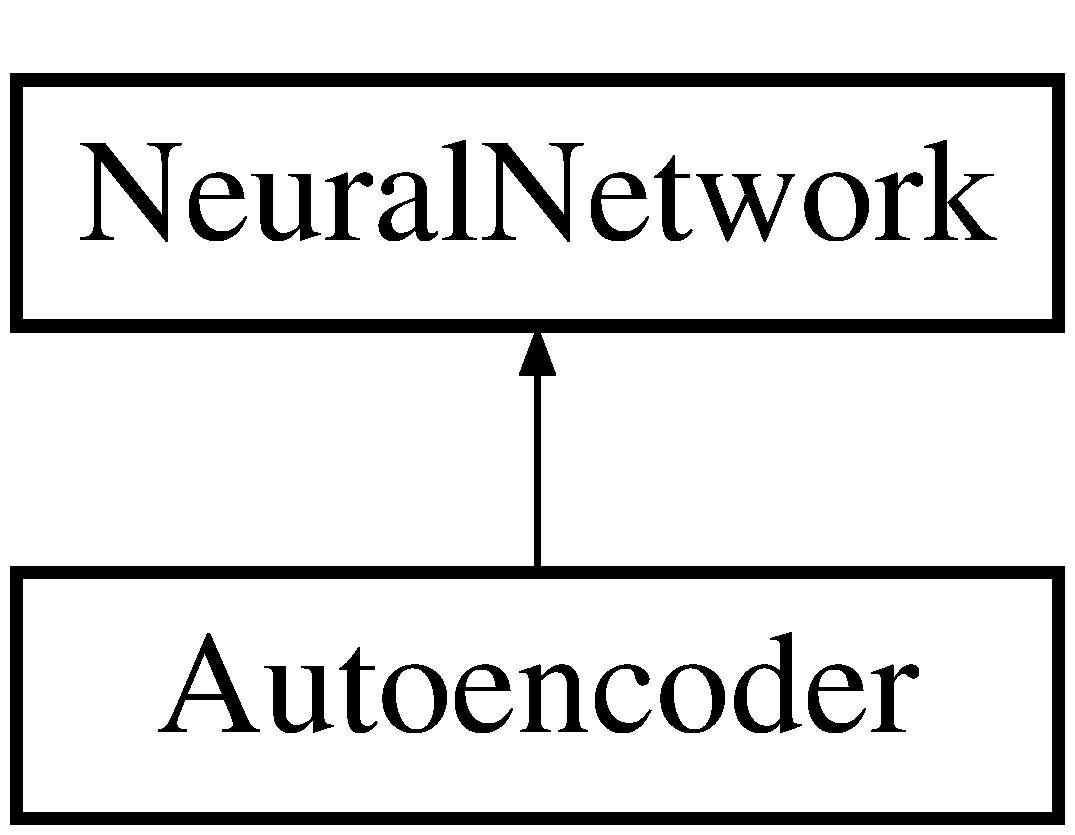
\includegraphics[height=2.000000cm]{classAutoencoder}
\end{center}
\end{figure}
\subsection*{Public Member Functions}
\begin{DoxyCompactItemize}
\item 
\hyperlink{classAutoencoder_a8749324f51cade4a1a21284f47097384}{$\sim$\+Autoencoder} ()
\item 
int \hyperlink{classAutoencoder_a4730a37272e51bef6c1a50efc9322fbe}{update\+Weights} (int ii, int jj, int kk, double learning\+Rate, double penalty)
\item 
int \hyperlink{classAutoencoder_aba5d429d35741aadbaf350364f64af7c}{update\+Weights\+Fast} (int ii, int jj, int kk, double learning\+Rate, double penalty)
\item 
int \hyperlink{classAutoencoder_a1a52083d0822fec947b93edf0797880f}{backpropagate} (double learning\+Rate, double lambda)
\item 
int \hyperlink{classAutoencoder_aa5832a7ff94e5af13d6fa41489796d82}{backpropagate\+Node\+Parallel} (double learning\+Rate, double lambda, int flag\+Release)
\item 
std\+::string \hyperlink{classAutoencoder_a0a306ad1b822c63cdcfe99a33233f7ea}{type} () const 
\begin{DoxyCompactList}\small\item\em Returns the type (string) of the autoencoder. \end{DoxyCompactList}\end{DoxyCompactItemize}
\subsection*{Additional Inherited Members}


\subsection{Detailed Description}
Class inherits functionality from Neural Network. 

Simple autoencoder. 

Definition at line 14 of file Autoencoder.\+h.



\subsection{Constructor \& Destructor Documentation}
\index{Autoencoder@{Autoencoder}!````~Autoencoder@{$\sim$\+Autoencoder}}
\index{````~Autoencoder@{$\sim$\+Autoencoder}!Autoencoder@{Autoencoder}}
\subsubsection[{\texorpdfstring{$\sim$\+Autoencoder()}{~Autoencoder()}}]{\setlength{\rightskip}{0pt plus 5cm}Autoencoder\+::$\sim$\+Autoencoder (
\begin{DoxyParamCaption}
{}
\end{DoxyParamCaption}
)}\hypertarget{classAutoencoder_a8749324f51cade4a1a21284f47097384}{}\label{classAutoencoder_a8749324f51cade4a1a21284f47097384}


Definition at line 108 of file autoencoder.\+cpp.



\subsection{Member Function Documentation}
\index{Autoencoder@{Autoencoder}!backpropagate@{backpropagate}}
\index{backpropagate@{backpropagate}!Autoencoder@{Autoencoder}}
\subsubsection[{\texorpdfstring{backpropagate(double learning\+Rate, double lambda)}{backpropagate(double learningRate, double lambda)}}]{\setlength{\rightskip}{0pt plus 5cm}int Autoencoder\+::backpropagate (
\begin{DoxyParamCaption}
\item[{double}]{learning\+Rate, }
\item[{double}]{lambda}
\end{DoxyParamCaption}
)\hspace{0.3cm}{\ttfamily [virtual]}}\hypertarget{classAutoencoder_a1a52083d0822fec947b93edf0797880f}{}\label{classAutoencoder_a1a52083d0822fec947b93edf0797880f}
The backpropagation algorithm 
\begin{DoxyParams}{Parameters}
{\em learning\+Rate} & -\/ the learning rate \\
\hline
{\em lambda} & -\/ the contractive autoencoder parameter \\
\hline
\end{DoxyParams}


Implements \hyperlink{classNeuralNetwork_af21bec3f1affe1a95346a57fd332f734}{Neural\+Network}.



Definition at line 4 of file autoencoder.\+cpp.

\index{Autoencoder@{Autoencoder}!backpropagate\+Node\+Parallel@{backpropagate\+Node\+Parallel}}
\index{backpropagate\+Node\+Parallel@{backpropagate\+Node\+Parallel}!Autoencoder@{Autoencoder}}
\subsubsection[{\texorpdfstring{backpropagate\+Node\+Parallel(double learning\+Rate, double lambda, int flag\+Release)}{backpropagateNodeParallel(double learningRate, double lambda, int flagRelease)}}]{\setlength{\rightskip}{0pt plus 5cm}int Autoencoder\+::backpropagate\+Node\+Parallel (
\begin{DoxyParamCaption}
\item[{double}]{learning\+Rate, }
\item[{double}]{lambda, }
\item[{int}]{flag\+Release}
\end{DoxyParamCaption}
)\hspace{0.3cm}{\ttfamily [virtual]}}\hypertarget{classAutoencoder_aa5832a7ff94e5af13d6fa41489796d82}{}\label{classAutoencoder_aa5832a7ff94e5af13d6fa41489796d82}
The backpropagation algorithm with parallel nodes 
\begin{DoxyParams}{Parameters}
{\em learning\+Rate} & -\/ the learning rate \\
\hline
{\em lambda} & -\/ the contractive autoencoder parameter \\
\hline
{\em flag\+Release} & -\/ 0 if the weights are to be released \\
\hline
\end{DoxyParams}


Implements \hyperlink{classNeuralNetwork_a01f72adec49e446ad4305bd6ad9859da}{Neural\+Network}.



Definition at line 20 of file autoencoder.\+cpp.

\index{Autoencoder@{Autoencoder}!type@{type}}
\index{type@{type}!Autoencoder@{Autoencoder}}
\subsubsection[{\texorpdfstring{type() const }{type() const }}]{\setlength{\rightskip}{0pt plus 5cm}std\+::string Autoencoder\+::type (
\begin{DoxyParamCaption}
{}
\end{DoxyParamCaption}
) const\hspace{0.3cm}{\ttfamily [inline]}, {\ttfamily [virtual]}}\hypertarget{classAutoencoder_a0a306ad1b822c63cdcfe99a33233f7ea}{}\label{classAutoencoder_a0a306ad1b822c63cdcfe99a33233f7ea}


Returns the type (string) of the autoencoder. 



Implements \hyperlink{classNeuralNetwork_aa3edc74bdbc4d8730c0fcc935dad2af0}{Neural\+Network}.



Definition at line 48 of file Autoencoder.\+h.

\index{Autoencoder@{Autoencoder}!update\+Weights@{update\+Weights}}
\index{update\+Weights@{update\+Weights}!Autoencoder@{Autoencoder}}
\subsubsection[{\texorpdfstring{update\+Weights(int ii, int jj, int kk, double learning\+Rate, double penalty)}{updateWeights(int ii, int jj, int kk, double learningRate, double penalty)}}]{\setlength{\rightskip}{0pt plus 5cm}int Autoencoder\+::update\+Weights (
\begin{DoxyParamCaption}
\item[{int}]{ii, }
\item[{int}]{jj, }
\item[{int}]{kk, }
\item[{double}]{learning\+Rate, }
\item[{double}]{penalty}
\end{DoxyParamCaption}
)\hspace{0.3cm}{\ttfamily [inline]}, {\ttfamily [virtual]}}\hypertarget{classAutoencoder_a4730a37272e51bef6c1a50efc9322fbe}{}\label{classAutoencoder_a4730a37272e51bef6c1a50efc9322fbe}
A function to update the weights with the gradient 
\begin{DoxyParams}{Parameters}
{\em ii} & layer \\
\hline
{\em jj} & node in the current layer \\
\hline
{\em kk} & node in the previous layer \\
\hline
{\em learning\+Rate} & learning rate \\
\hline
{\em penalty} & lambda for the contractive autoencoder \\
\hline
\end{DoxyParams}


Implements \hyperlink{classNeuralNetwork_acd83d73dbae85f80c1173bdb53e37726}{Neural\+Network}.



Definition at line 89 of file autoencoder.\+cpp.

\index{Autoencoder@{Autoencoder}!update\+Weights\+Fast@{update\+Weights\+Fast}}
\index{update\+Weights\+Fast@{update\+Weights\+Fast}!Autoencoder@{Autoencoder}}
\subsubsection[{\texorpdfstring{update\+Weights\+Fast(int ii, int jj, int kk, double learning\+Rate, double penalty)}{updateWeightsFast(int ii, int jj, int kk, double learningRate, double penalty)}}]{\setlength{\rightskip}{0pt plus 5cm}int Autoencoder\+::update\+Weights\+Fast (
\begin{DoxyParamCaption}
\item[{int}]{ii, }
\item[{int}]{jj, }
\item[{int}]{kk, }
\item[{double}]{learning\+Rate, }
\item[{double}]{penalty}
\end{DoxyParamCaption}
)\hspace{0.3cm}{\ttfamily [inline]}, {\ttfamily [virtual]}}\hypertarget{classAutoencoder_aba5d429d35741aadbaf350364f64af7c}{}\label{classAutoencoder_aba5d429d35741aadbaf350364f64af7c}
A function to update the weights with the gradient (fast, no redundunt calculations for momentum and ada\+Grad if both are not used) 
\begin{DoxyParams}{Parameters}
{\em ii} & layer \\
\hline
{\em jj} & node in the current layer \\
\hline
{\em kk} & node in the previous layer \\
\hline
{\em learning\+Rate} & learning rate \\
\hline
{\em penalty} & lambda for the contractive autoencoder \\
\hline
\end{DoxyParams}


Implements \hyperlink{classNeuralNetwork_a1bc1c063c3048b0551ae92352b553060}{Neural\+Network}.



Definition at line 78 of file autoencoder.\+cpp.



The documentation for this class was generated from the following files\+:\begin{DoxyCompactItemize}
\item 
src/headers/\hyperlink{Autoencoder_8h}{Autoencoder.\+h}\item 
src/cpp/\hyperlink{autoencoder_8cpp}{autoencoder.\+cpp}\end{DoxyCompactItemize}

\hypertarget{classContractiveAutoencoder}{}\section{Contractive\+Autoencoder Class Reference}
\label{classContractiveAutoencoder}\index{Contractive\+Autoencoder@{Contractive\+Autoencoder}}


Class inherets functions from the Neural Network class.  




{\ttfamily \#include \char`\"{}Contractive\+Autoencoder.\+h\char`\"{}}

Inheritance diagram for Contractive\+Autoencoder\+:\begin{figure}[H]
\begin{center}
\leavevmode
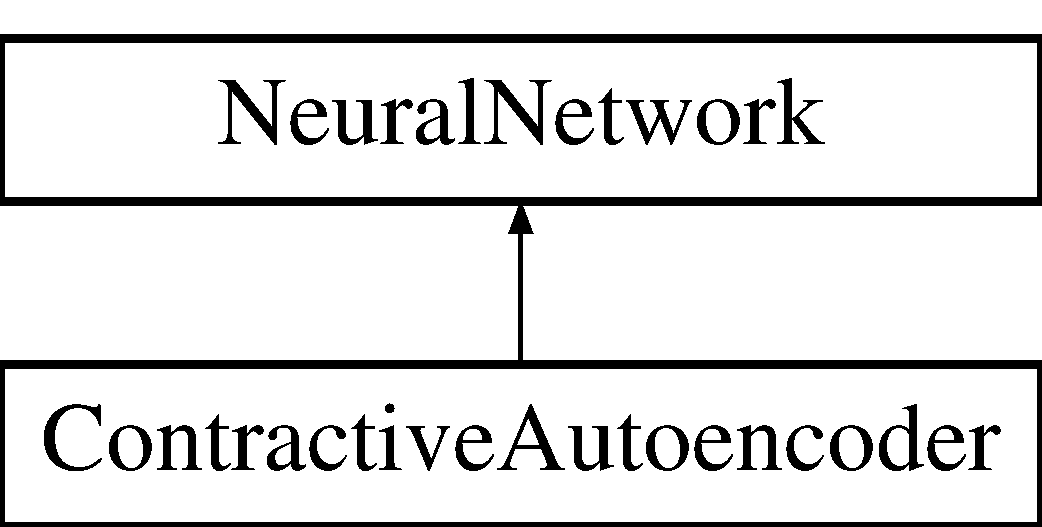
\includegraphics[height=2.000000cm]{classContractiveAutoencoder}
\end{center}
\end{figure}
\subsection*{Public Member Functions}
\begin{DoxyCompactItemize}
\item 
\hyperlink{classContractiveAutoencoder_a0817944843aa751ae7391d36d9f7a717}{$\sim$\+Contractive\+Autoencoder} ()
\item 
int \hyperlink{classContractiveAutoencoder_ab10b3558c21939bed2654a0110b6bc08}{update\+Weights} (int ii, int jj, int kk, double val, double penalty)
\item 
int \hyperlink{classContractiveAutoencoder_a66faa7d13437de0e864a6adec9994cd8}{update\+Weights\+Fast} (int ii, int jj, int kk, double val, double penalty)
\item 
int \hyperlink{classContractiveAutoencoder_a66bf959d85d09b2f5cc2e06d6bdfe6bf}{backpropagate} (double learning\+Rate, double lambda)
\item 
int \hyperlink{classContractiveAutoencoder_a65daf5136737423ee6b0fd89442cbf70}{backpropagate\+Node\+Parallel} (double learning\+Rate, double lambda, int)
\item 
std\+::string \hyperlink{classContractiveAutoencoder_a8db3fc9434f66e1a7e036a49f2d19ac6}{type} () const 
\begin{DoxyCompactList}\small\item\em Returns the type (string) of the autoencoder. \end{DoxyCompactList}\end{DoxyCompactItemize}
\subsection*{Additional Inherited Members}


\subsection{Detailed Description}
Class inherets functions from the Neural Network class. 

The main difference is in backpropagation function, which needs to accomodate calculations associated with the penalty term. 

Definition at line 12 of file Contractive\+Autoencoder.\+h.



\subsection{Constructor \& Destructor Documentation}
\index{Contractive\+Autoencoder@{Contractive\+Autoencoder}!````~Contractive\+Autoencoder@{$\sim$\+Contractive\+Autoencoder}}
\index{````~Contractive\+Autoencoder@{$\sim$\+Contractive\+Autoencoder}!Contractive\+Autoencoder@{Contractive\+Autoencoder}}
\subsubsection[{\texorpdfstring{$\sim$\+Contractive\+Autoencoder()}{~ContractiveAutoencoder()}}]{\setlength{\rightskip}{0pt plus 5cm}Contractive\+Autoencoder\+::$\sim$\+Contractive\+Autoencoder (
\begin{DoxyParamCaption}
{}
\end{DoxyParamCaption}
)}\hypertarget{classContractiveAutoencoder_a0817944843aa751ae7391d36d9f7a717}{}\label{classContractiveAutoencoder_a0817944843aa751ae7391d36d9f7a717}


Definition at line 112 of file contractiveautoencoder.\+cpp.



\subsection{Member Function Documentation}
\index{Contractive\+Autoencoder@{Contractive\+Autoencoder}!backpropagate@{backpropagate}}
\index{backpropagate@{backpropagate}!Contractive\+Autoencoder@{Contractive\+Autoencoder}}
\subsubsection[{\texorpdfstring{backpropagate(double learning\+Rate, double lambda)}{backpropagate(double learningRate, double lambda)}}]{\setlength{\rightskip}{0pt plus 5cm}int Contractive\+Autoencoder\+::backpropagate (
\begin{DoxyParamCaption}
\item[{double}]{learning\+Rate, }
\item[{double}]{lambda}
\end{DoxyParamCaption}
)\hspace{0.3cm}{\ttfamily [virtual]}}\hypertarget{classContractiveAutoencoder_a66bf959d85d09b2f5cc2e06d6bdfe6bf}{}\label{classContractiveAutoencoder_a66bf959d85d09b2f5cc2e06d6bdfe6bf}
The backpropagation algorithm 
\begin{DoxyParams}{Parameters}
{\em learning\+Rate} & -\/ the learning rate \\
\hline
{\em lambda} & -\/ the contractive autoencoder parameter \\
\hline
\end{DoxyParams}


Implements \hyperlink{classNeuralNetwork_af21bec3f1affe1a95346a57fd332f734}{Neural\+Network}.



Definition at line 50 of file contractiveautoencoder.\+cpp.

\index{Contractive\+Autoencoder@{Contractive\+Autoencoder}!backpropagate\+Node\+Parallel@{backpropagate\+Node\+Parallel}}
\index{backpropagate\+Node\+Parallel@{backpropagate\+Node\+Parallel}!Contractive\+Autoencoder@{Contractive\+Autoencoder}}
\subsubsection[{\texorpdfstring{backpropagate\+Node\+Parallel(double learning\+Rate, double lambda, int)}{backpropagateNodeParallel(double learningRate, double lambda, int)}}]{\setlength{\rightskip}{0pt plus 5cm}int Contractive\+Autoencoder\+::backpropagate\+Node\+Parallel (
\begin{DoxyParamCaption}
\item[{double}]{learning\+Rate, }
\item[{double}]{lambda, }
\item[{int}]{a}
\end{DoxyParamCaption}
)\hspace{0.3cm}{\ttfamily [virtual]}}\hypertarget{classContractiveAutoencoder_a65daf5136737423ee6b0fd89442cbf70}{}\label{classContractiveAutoencoder_a65daf5136737423ee6b0fd89442cbf70}
The backpropagation algorithm with parallel nodes 
\begin{DoxyParams}{Parameters}
{\em learning\+Rate} & -\/ the learning rate \\
\hline
{\em lambda} & -\/ the contractive autoencoder parameter \\
\hline
{\em flag\+Release} & -\/ 0 if the weights are to be released \\
\hline
\end{DoxyParams}


Implements \hyperlink{classNeuralNetwork_a01f72adec49e446ad4305bd6ad9859da}{Neural\+Network}.



Definition at line 5 of file contractiveautoencoder.\+cpp.

\index{Contractive\+Autoencoder@{Contractive\+Autoencoder}!type@{type}}
\index{type@{type}!Contractive\+Autoencoder@{Contractive\+Autoencoder}}
\subsubsection[{\texorpdfstring{type() const }{type() const }}]{\setlength{\rightskip}{0pt plus 5cm}std\+::string Contractive\+Autoencoder\+::type (
\begin{DoxyParamCaption}
{}
\end{DoxyParamCaption}
) const\hspace{0.3cm}{\ttfamily [inline]}, {\ttfamily [virtual]}}\hypertarget{classContractiveAutoencoder_a8db3fc9434f66e1a7e036a49f2d19ac6}{}\label{classContractiveAutoencoder_a8db3fc9434f66e1a7e036a49f2d19ac6}


Returns the type (string) of the autoencoder. 



Implements \hyperlink{classNeuralNetwork_aa3edc74bdbc4d8730c0fcc935dad2af0}{Neural\+Network}.



Definition at line 46 of file Contractive\+Autoencoder.\+h.

\index{Contractive\+Autoencoder@{Contractive\+Autoencoder}!update\+Weights@{update\+Weights}}
\index{update\+Weights@{update\+Weights}!Contractive\+Autoencoder@{Contractive\+Autoencoder}}
\subsubsection[{\texorpdfstring{update\+Weights(int ii, int jj, int kk, double val, double penalty)}{updateWeights(int ii, int jj, int kk, double val, double penalty)}}]{\setlength{\rightskip}{0pt plus 5cm}int Contractive\+Autoencoder\+::update\+Weights (
\begin{DoxyParamCaption}
\item[{int}]{ii, }
\item[{int}]{jj, }
\item[{int}]{kk, }
\item[{double}]{val, }
\item[{double}]{penalty}
\end{DoxyParamCaption}
)\hspace{0.3cm}{\ttfamily [inline]}, {\ttfamily [virtual]}}\hypertarget{classContractiveAutoencoder_ab10b3558c21939bed2654a0110b6bc08}{}\label{classContractiveAutoencoder_ab10b3558c21939bed2654a0110b6bc08}
A function to update the weights with the gradient 
\begin{DoxyParams}{Parameters}
{\em ii} & layer \\
\hline
{\em jj} & node in the current layer \\
\hline
{\em kk} & node in the previous layer \\
\hline
{\em learning\+Rate} & learning rate \\
\hline
{\em penalty} & lambda for the contractive autoencoder \\
\hline
\end{DoxyParams}


Implements \hyperlink{classNeuralNetwork_acd83d73dbae85f80c1173bdb53e37726}{Neural\+Network}.



Definition at line 106 of file contractiveautoencoder.\+cpp.

\index{Contractive\+Autoencoder@{Contractive\+Autoencoder}!update\+Weights\+Fast@{update\+Weights\+Fast}}
\index{update\+Weights\+Fast@{update\+Weights\+Fast}!Contractive\+Autoencoder@{Contractive\+Autoencoder}}
\subsubsection[{\texorpdfstring{update\+Weights\+Fast(int ii, int jj, int kk, double val, double penalty)}{updateWeightsFast(int ii, int jj, int kk, double val, double penalty)}}]{\setlength{\rightskip}{0pt plus 5cm}int Contractive\+Autoencoder\+::update\+Weights\+Fast (
\begin{DoxyParamCaption}
\item[{int}]{ii, }
\item[{int}]{jj, }
\item[{int}]{kk, }
\item[{double}]{val, }
\item[{double}]{penalty}
\end{DoxyParamCaption}
)\hspace{0.3cm}{\ttfamily [inline]}, {\ttfamily [virtual]}}\hypertarget{classContractiveAutoencoder_a66faa7d13437de0e864a6adec9994cd8}{}\label{classContractiveAutoencoder_a66faa7d13437de0e864a6adec9994cd8}
A function to update the weights with the gradient (fast, no redundunt calculations for momentum and ada\+Grad if both are not used) 
\begin{DoxyParams}{Parameters}
{\em ii} & layer \\
\hline
{\em jj} & node in the current layer \\
\hline
{\em kk} & node in the previous layer \\
\hline
{\em learning\+Rate} & learning rate \\
\hline
{\em penalty} & lambda for the contractive autoencoder \\
\hline
\end{DoxyParams}


Implements \hyperlink{classNeuralNetwork_a1bc1c063c3048b0551ae92352b553060}{Neural\+Network}.



Definition at line 100 of file contractiveautoencoder.\+cpp.



The documentation for this class was generated from the following files\+:\begin{DoxyCompactItemize}
\item 
src/headers/\hyperlink{ContractiveAutoencoder_8h}{Contractive\+Autoencoder.\+h}\item 
src/cpp/\hyperlink{contractiveautoencoder_8cpp}{contractiveautoencoder.\+cpp}\end{DoxyCompactItemize}

\hypertarget{classDataReader}{}\section{Data\+Reader Class Reference}
\label{classDataReader}\index{Data\+Reader@{Data\+Reader}}


{\ttfamily \#include \char`\"{}Data\+Reader.\+h\char`\"{}}

\subsection*{Public Member Functions}
\begin{DoxyCompactItemize}
\item 
int \hyperlink{classDataReader_a3af651bdeb6b8613b5c1e5c20d135fee}{read\+Data\+Train} (vector$<$ double $>$ $\ast$data\+Train\+In, int $\ast$numb\+In, int $\ast$numb\+It\+Train, vector$<$ double $>$ $\ast$mask\+Rearanged\+Train, int $\ast$x\+Width\+Train, int $\ast$y\+Width\+Train)
\item 
int \hyperlink{classDataReader_a9816af31c4b15b59379622346d3782f7}{read\+Data\+Test} (vector$<$ double $>$ $\ast$data\+Test\+In, int $\ast$numb\+It\+Test, vector$<$ double $>$ $\ast$mask\+Rearanged, vector$<$ double $>$ $\ast$mask\+Rearanged\+Validation)
\item 
int \hyperlink{classDataReader_adc671d5bc1196eb8a99b37d7f87440de}{write\+Data\+Cube} (vector$<$ double $>$ data, std\+::string path, double flag\+Mask)
\item 
void \hyperlink{classDataReader_af0251b5edd10a372d9f30a836472357f}{zero\+Cube} ()
\begin{DoxyCompactList}\small\item\em A function used to set all the values of the data cubes to zero. \end{DoxyCompactList}\item 
void \hyperlink{classDataReader_a3cbc317ede9f646ec01f5cacf90781a0}{write\+Cube\+Into\+File} (std\+::string path, double flag\+Mask)
\item 
int \hyperlink{classDataReader_aa2f408b750df89a6d6ab2a0ce286a914}{write\+Data\+Cube\+Prediction} (vector$<$ double $>$ data\+Target, vector$<$ double $>$ data\+Pred, std\+::string path)
\item 
double \hyperlink{classDataReader_a22c2992f3d00c30f9b53e46a6a38571f}{calculate\+Coefficient\+Cube} ()
\item 
int \hyperlink{classDataReader_ae6645eba51e680bd59cc3c9fe297e5b5}{check\+Dimensions\+Patch} ()
\begin{DoxyCompactList}\small\item\em A sensibility check function for the dimentions of the Patch. \end{DoxyCompactList}\item 
int \hyperlink{classDataReader_af6056c45ad47ad45ab8e6663280e55fc}{check\+Dimensions\+Mask} ()
\begin{DoxyCompactList}\small\item\em A sensibility check function for the dimentions of the Mask. \end{DoxyCompactList}\item 
int \hyperlink{classDataReader_a28b365a9335395e679c56074c56262d3}{calculate\+Bounds} (int train\+Flag, int $\ast$start\+Y\+Width, int $\ast$start\+X\+Width, int $\ast$start\+Z\+Width, int ii, int $\ast$numb\+Iterations)
\item 
int \hyperlink{classDataReader_afb618b0fafa0acb2365509a122f3602a}{initialise} (\hyperlink{classParamsInit}{Params\+Init} parameters)
\item 
int \hyperlink{classDataReader_aefcb38bd08e3941a328ff64aa558e7a8}{read\+Train\+Cube} ()
\begin{DoxyCompactList}\small\item\em A function to read the Training cube from the file. \end{DoxyCompactList}\item 
int \hyperlink{classDataReader_a6fda577c7a39231af8ff7bad9821dd94}{read\+Test\+Cube} ()
\begin{DoxyCompactList}\small\item\em A function to read the Test cube from the file. \end{DoxyCompactList}\item 
int \hyperlink{classDataReader_abad2eb24821cb6097c7eb9e017d0123f}{read\+Masks} ()
\begin{DoxyCompactList}\small\item\em A function to read the mask from the file. \end{DoxyCompactList}\item 
double \hyperlink{classDataReader_a1384d31286da6be6715687ecf5ebbc58}{calculate\+S\+NR} (vector$<$ double $>$ data\+Clean, vector$<$ double $>$ data\+Predicted, std\+::string path)
\end{DoxyCompactItemize}
\subsection*{Private Types}
\begin{DoxyCompactItemize}
\item 
enum \hyperlink{classDataReader_a4d7ac2e743b4d00d62ce3ac86dd35f76}{Flag} \{ \hyperlink{classDataReader_a4d7ac2e743b4d00d62ce3ac86dd35f76aac0022634ec9e261a5f03eebe88fed11}{disabled}, 
\hyperlink{classDataReader_a4d7ac2e743b4d00d62ce3ac86dd35f76a469181e07fca749b48a38f7c7ed9b619}{enabled}
 \}\begin{DoxyCompactList}\small\item\em A flag (more verbal than 0 and 1) \end{DoxyCompactList}
\end{DoxyCompactItemize}
\subsection*{Private Attributes}
\begin{DoxyCompactItemize}
\item 
\hyperlink{classDataReader_a4d7ac2e743b4d00d62ce3ac86dd35f76}{Flag} \hyperlink{classDataReader_a047fea2d4cf25627f3df820b560d95be}{m\+\_\+flag\+Mask\+Validation}
\begin{DoxyCompactList}\small\item\em Enabled if validation mask is used. \end{DoxyCompactList}\item 
\hyperlink{classDataReader_a4d7ac2e743b4d00d62ce3ac86dd35f76}{Flag} \hyperlink{classDataReader_a71945ad4af9366b1d4060d49e01e34f9}{m\+\_\+flag\+Mask\+Test}
\begin{DoxyCompactList}\small\item\em Enabled if test mask is used. \end{DoxyCompactList}\item 
\hyperlink{classDataReader_a4d7ac2e743b4d00d62ce3ac86dd35f76}{Flag} \hyperlink{classDataReader_a09cceda2cf4ac5522c6e05b1424660d4}{m\+\_\+augment\+Flag}
\begin{DoxyCompactList}\small\item\em Enabled if augmentation is used. \end{DoxyCompactList}\item 
std\+::string \hyperlink{classDataReader_a0fe9a400035e0ce40b7f9adee9759fd3}{m\+\_\+name\+Data\+Train\+In}
\begin{DoxyCompactList}\small\item\em A path to the training data. \end{DoxyCompactList}\item 
std\+::string \hyperlink{classDataReader_ad1604383cd367336e8d3aa00ef3b4396}{m\+\_\+name\+Data\+Test\+In}
\begin{DoxyCompactList}\small\item\em A path to the test data. \end{DoxyCompactList}\item 
std\+::string \hyperlink{classDataReader_ad0b4aa478a29fe29c71230d6ba1582ce}{m\+\_\+name\+Mask\+Test}
\begin{DoxyCompactList}\small\item\em A path to the test mask. \end{DoxyCompactList}\item 
std\+::string \hyperlink{classDataReader_a5b59718d2007d1bb2f7b502788df8752}{m\+\_\+name\+Mask\+Validation}
\begin{DoxyCompactList}\small\item\em A path to the validation mask. \end{DoxyCompactList}\item 
vector$<$ vector$<$ vector$<$ double $>$ $>$ $>$ \hyperlink{classDataReader_a27c2e4c67ca778cb720a3d56beb8ee7f}{m\+\_\+coef\+Cube}
\item 
vector$<$ vector$<$ vector$<$ double $>$ $>$ $>$ \hyperlink{classDataReader_a0a9bb36b0b16402e27008f4327e1bb92}{m\+\_\+cube}
\begin{DoxyCompactList}\small\item\em A cube with final (predicted values) \end{DoxyCompactList}\item 
vector$<$ vector$<$ vector$<$ double $>$ $>$ $>$ \hyperlink{classDataReader_a3647b5fff6dff6a92c8f2f83dfcfa055}{m\+\_\+cube\+Clean}
\begin{DoxyCompactList}\small\item\em A cube with clean data to write. \end{DoxyCompactList}\item 
vector$<$ vector$<$ double $>$ $>$ \hyperlink{classDataReader_afadf320f5ab08a34b8b06c839a8192e0}{m\+\_\+mask\+Validation}
\begin{DoxyCompactList}\small\item\em A matrix to hold validation mask. \end{DoxyCompactList}\item 
vector$<$ vector$<$ double $>$ $>$ \hyperlink{classDataReader_a8eb1e7630b4efd101708fb3b5a6856c6}{m\+\_\+mask}
\begin{DoxyCompactList}\small\item\em A matrix to hold the mask for test and traing (real missing values) \end{DoxyCompactList}\item 
double \hyperlink{classDataReader_a4dbda7a5c05acd673c2188ef37913e40}{m\+\_\+input\+Scale}
\item 
double \hyperlink{classDataReader_ad2afd61ea40bdaa3d6678adc1548a057}{m\+\_\+max}
\begin{DoxyCompactList}\small\item\em Maximum value of the seismic data cube. \end{DoxyCompactList}\item 
double \hyperlink{classDataReader_aba740a2b8be42c25449e1c91e0e03805}{m\+\_\+min}
\begin{DoxyCompactList}\small\item\em Minimum value of the seismic data cube. \end{DoxyCompactList}\item 
double \hyperlink{classDataReader_a9a9066f2dafe278b3acd45e84cc2126e}{m\+\_\+max\+Abs}
\begin{DoxyCompactList}\small\item\em Maximum absolute value of the seismic data cube. \end{DoxyCompactList}\item 
double \hyperlink{classDataReader_aeb1b06be9af5ea726e9b8ad11b5b34f1}{m\+\_\+\+M\+S\+Error}
\begin{DoxyCompactList}\small\item\em Total M\+SE error of the reconstruction. \end{DoxyCompactList}\item 
double \hyperlink{classDataReader_a5bba6f4ec228522330fda878214f7395}{m\+\_\+q\+Measure}
\begin{DoxyCompactList}\small\item\em S\+NR measure of the reconstructed cube (see Georgious paper) \end{DoxyCompactList}\item 
int \hyperlink{classDataReader_ae74053a5592498d373fc12254145ce39}{m\+\_\+z\+Width\+Train}
\begin{DoxyCompactList}\small\item\em Z dimention of the Train Cube. \end{DoxyCompactList}\item 
int \hyperlink{classDataReader_a0c4b86a80694b557fe1509b615b76244}{m\+\_\+x\+Width\+Train}
\begin{DoxyCompactList}\small\item\em X dimention of the Train Cube. \end{DoxyCompactList}\item 
int \hyperlink{classDataReader_a4a627c7884969007b149ce1023ee3e11}{m\+\_\+y\+Width\+Train}
\begin{DoxyCompactList}\small\item\em Y dimention of the Train Cube. \end{DoxyCompactList}\item 
int \hyperlink{classDataReader_a2c029cc64a4c674ee19477c9bfcc2ae6}{m\+\_\+z\+Width\+Test}
\begin{DoxyCompactList}\small\item\em Z dimention of the Test Cube. \end{DoxyCompactList}\item 
int \hyperlink{classDataReader_a3b70edeb59564609bc13d11761586225}{m\+\_\+x\+Width\+Test}
\begin{DoxyCompactList}\small\item\em X dimention of the Test Cube. \end{DoxyCompactList}\item 
int \hyperlink{classDataReader_ac8debe3d06ff92d1d57e90bb5d18a812}{m\+\_\+y\+Width\+Test}
\begin{DoxyCompactList}\small\item\em Y dimention of the Test Cube. \end{DoxyCompactList}\item 
int \hyperlink{classDataReader_a95d075ccc3b12ec30a97d6664642efc2}{m\+\_\+patchX}
\begin{DoxyCompactList}\small\item\em Size of the patch in X dimention. \end{DoxyCompactList}\item 
int \hyperlink{classDataReader_a68b54683e0e0581e3dd76874ea5b6941}{m\+\_\+patchZ}
\begin{DoxyCompactList}\small\item\em Size of the patch in Z dimention. \end{DoxyCompactList}\item 
int \hyperlink{classDataReader_aed3b404cf78c6973363402e5e871e46a}{m\+\_\+patchY}
\begin{DoxyCompactList}\small\item\em Size of the patch in Y dimention. \end{DoxyCompactList}\item 
int \hyperlink{classDataReader_a6d2cc22f742392bafb485fe0f07b13e8}{m\+\_\+shift\+X\+Train}
\begin{DoxyCompactList}\small\item\em Shift in X dimention of the patch while training. \end{DoxyCompactList}\item 
int \hyperlink{classDataReader_a2d564c01ed2225f2c853063113ef87b8}{m\+\_\+shift\+Y\+Train}
\begin{DoxyCompactList}\small\item\em Shift in Y dimention of the patch while training. \end{DoxyCompactList}\item 
int \hyperlink{classDataReader_a0edec69c662462ca0189a5a47a567596}{m\+\_\+shift\+Z\+Train}
\begin{DoxyCompactList}\small\item\em Shift in Z dimention of the patch while training. \end{DoxyCompactList}\item 
int \hyperlink{classDataReader_a066a1c0f512fccdb2b21d23cce551ee7}{m\+\_\+shift\+X\+Test}
\begin{DoxyCompactList}\small\item\em Shift in X dimention of the patch while testing. \end{DoxyCompactList}\item 
int \hyperlink{classDataReader_ab5002c766c4cebca361dd21f1d2cbc86}{m\+\_\+shift\+Y\+Test}
\begin{DoxyCompactList}\small\item\em Shift in Y dimention of the patch while testing. \end{DoxyCompactList}\item 
int \hyperlink{classDataReader_a9f9ae5a90b34758f37671671e1f002f7}{m\+\_\+shift\+Z\+Test}
\begin{DoxyCompactList}\small\item\em Shift in Z dimention of the patch while testing. \end{DoxyCompactList}\item 
int \hyperlink{classDataReader_a1a78f7b37cb3908c3db5ee4538c2c932}{m\+\_\+numb\+It\+Train}
\begin{DoxyCompactList}\small\item\em Number of training iterations. \end{DoxyCompactList}\item 
int \hyperlink{classDataReader_a9a9f00295f7d5aaca78539802fe09c6c}{m\+\_\+numb\+It\+Test}
\begin{DoxyCompactList}\small\item\em Number of test iterations. \end{DoxyCompactList}\item 
int \hyperlink{classDataReader_a9ae84cb0ea7dd165616880737280e6b6}{m\+\_\+patch\+Size}
\begin{DoxyCompactList}\small\item\em Total patch size (m\+\_\+patch\+X$\ast$m\+\_\+patch\+Y$\ast$m\+\_\+patchZ) \end{DoxyCompactList}\item 
int \hyperlink{classDataReader_a1a13928367a9c5d02f6e11d2d742e429}{m\+\_\+tot\+Cubes\+Test}
\begin{DoxyCompactList}\small\item\em Total number of test examples. \end{DoxyCompactList}\item 
int \hyperlink{classDataReader_af20e42b5dc09a33b2c2704cb58d01803}{m\+\_\+x\+Width\+Mask}
\begin{DoxyCompactList}\small\item\em Width of the mask in X dimention. \end{DoxyCompactList}\item 
int \hyperlink{classDataReader_aa381a07a34d528a39ae493aba4d42521}{m\+\_\+y\+Width\+Mask}
\begin{DoxyCompactList}\small\item\em Width of the mask in Y direction. \end{DoxyCompactList}\item 
int \hyperlink{classDataReader_a3857860c363d6127fc8b6b54fd53d81f}{m\+\_\+augmentX}
\begin{DoxyCompactList}\small\item\em Size of the band of additional values in X direction. \end{DoxyCompactList}\item 
int \hyperlink{classDataReader_a139941a6fc5ba0546a1ddb892b2ec958}{m\+\_\+augmentY}
\begin{DoxyCompactList}\small\item\em Size of the band of additional values in Y direction. \end{DoxyCompactList}\item 
int \hyperlink{classDataReader_a71318eba05d2c7dbf8ac6bd804f5d5da}{m\+\_\+augmentZ}
\begin{DoxyCompactList}\small\item\em Size of the band of additional values in Z direction. \end{DoxyCompactList}\end{DoxyCompactItemize}


\subsection{Detailed Description}


Definition at line 21 of file Data\+Reader.\+h.



\subsection{Member Enumeration Documentation}
\index{Data\+Reader@{Data\+Reader}!Flag@{Flag}}
\index{Flag@{Flag}!Data\+Reader@{Data\+Reader}}
\subsubsection[{\texorpdfstring{Flag}{Flag}}]{\setlength{\rightskip}{0pt plus 5cm}enum {\bf Data\+Reader\+::\+Flag}\hspace{0.3cm}{\ttfamily [private]}}\hypertarget{classDataReader_a4d7ac2e743b4d00d62ce3ac86dd35f76}{}\label{classDataReader_a4d7ac2e743b4d00d62ce3ac86dd35f76}


A flag (more verbal than 0 and 1) 

\begin{Desc}
\item[Enumerator]\par
\begin{description}
\index{disabled@{disabled}!Data\+Reader@{Data\+Reader}}\index{Data\+Reader@{Data\+Reader}!disabled@{disabled}}\item[{\em 
disabled\hypertarget{classDataReader_a4d7ac2e743b4d00d62ce3ac86dd35f76aac0022634ec9e261a5f03eebe88fed11}{}\label{classDataReader_a4d7ac2e743b4d00d62ce3ac86dd35f76aac0022634ec9e261a5f03eebe88fed11}
}]\index{enabled@{enabled}!Data\+Reader@{Data\+Reader}}\index{Data\+Reader@{Data\+Reader}!enabled@{enabled}}\item[{\em 
enabled\hypertarget{classDataReader_a4d7ac2e743b4d00d62ce3ac86dd35f76a469181e07fca749b48a38f7c7ed9b619}{}\label{classDataReader_a4d7ac2e743b4d00d62ce3ac86dd35f76a469181e07fca749b48a38f7c7ed9b619}
}]\end{description}
\end{Desc}


Definition at line 25 of file Data\+Reader.\+h.



\subsection{Member Function Documentation}
\index{Data\+Reader@{Data\+Reader}!calculate\+Bounds@{calculate\+Bounds}}
\index{calculate\+Bounds@{calculate\+Bounds}!Data\+Reader@{Data\+Reader}}
\subsubsection[{\texorpdfstring{calculate\+Bounds(int train\+Flag, int $\ast$start\+Y\+Width, int $\ast$start\+X\+Width, int $\ast$start\+Z\+Width, int ii, int $\ast$numb\+Iterations)}{calculateBounds(int trainFlag, int *startYWidth, int *startXWidth, int *startZWidth, int ii, int *numbIterations)}}]{\setlength{\rightskip}{0pt plus 5cm}int Data\+Reader\+::calculate\+Bounds (
\begin{DoxyParamCaption}
\item[{int}]{train\+Flag, }
\item[{int $\ast$}]{start\+Y\+Width, }
\item[{int $\ast$}]{start\+X\+Width, }
\item[{int $\ast$}]{start\+Z\+Width, }
\item[{int}]{ii, }
\item[{int $\ast$}]{numb\+Iterations}
\end{DoxyParamCaption}
)}\hypertarget{classDataReader_a28b365a9335395e679c56074c56262d3}{}\label{classDataReader_a28b365a9335395e679c56074c56262d3}
A function used to map the cube coefficients to the coefficients of the patches 
\begin{DoxyParams}{Parameters}
{\em train\+Flag} & -\/ set to 1 if called from the function calculating bounds for training patches \\
\hline
{\em start\+Y\+Width} & -\/ starting index in the Y in the data cube from where the patch is taken \\
\hline
{\em start\+X\+Width} & -\/ starting index in the X in the data cube from where the patch is taken \\
\hline
{\em start\+Z\+Width} & -\/ starting index in the Z in the data cube from where the patch is taken \\
\hline
{\em ii} & -\/ current iteration of the \\
\hline
{\em numb\+Iterations} & -\/ total number of patches \\
\hline
\end{DoxyParams}


Definition at line 338 of file datareader.\+cpp.

\index{Data\+Reader@{Data\+Reader}!calculate\+Coefficient\+Cube@{calculate\+Coefficient\+Cube}}
\index{calculate\+Coefficient\+Cube@{calculate\+Coefficient\+Cube}!Data\+Reader@{Data\+Reader}}
\subsubsection[{\texorpdfstring{calculate\+Coefficient\+Cube()}{calculateCoefficientCube()}}]{\setlength{\rightskip}{0pt plus 5cm}double Data\+Reader\+::calculate\+Coefficient\+Cube (
\begin{DoxyParamCaption}
{}
\end{DoxyParamCaption}
)}\hypertarget{classDataReader_a22c2992f3d00c30f9b53e46a6a38571f}{}\label{classDataReader_a22c2992f3d00c30f9b53e46a6a38571f}
A function to calculate the values stored in m\+\_\+coef\+Cube, used to scale the overlapping patches in the final data cube 

Definition at line 393 of file datareader.\+cpp.

\index{Data\+Reader@{Data\+Reader}!calculate\+S\+NR@{calculate\+S\+NR}}
\index{calculate\+S\+NR@{calculate\+S\+NR}!Data\+Reader@{Data\+Reader}}
\subsubsection[{\texorpdfstring{calculate\+S\+N\+R(vector$<$ double $>$ data\+Clean, vector$<$ double $>$ data\+Predicted, std\+::string path)}{calculateSNR(vector< double > dataClean, vector< double > dataPredicted, std::string path)}}]{\setlength{\rightskip}{0pt plus 5cm}double Data\+Reader\+::calculate\+S\+NR (
\begin{DoxyParamCaption}
\item[{vector$<$ double $>$}]{data\+Clean, }
\item[{vector$<$ double $>$}]{data\+Predicted, }
\item[{std\+::string}]{path}
\end{DoxyParamCaption}
)}\hypertarget{classDataReader_a1384d31286da6be6715687ecf5ebbc58}{}\label{classDataReader_a1384d31286da6be6715687ecf5ebbc58}
A function to calculate the S\+NR 
\begin{DoxyParams}{Parameters}
{\em data\+Clean} & target data \\
\hline
{\em data\+Predicted} & predicted data \\
\hline
{\em path} & -\/ path to the file where to write the S\+NR \\
\hline
\end{DoxyParams}


Definition at line 433 of file datareader.\+cpp.

\index{Data\+Reader@{Data\+Reader}!check\+Dimensions\+Mask@{check\+Dimensions\+Mask}}
\index{check\+Dimensions\+Mask@{check\+Dimensions\+Mask}!Data\+Reader@{Data\+Reader}}
\subsubsection[{\texorpdfstring{check\+Dimensions\+Mask()}{checkDimensionsMask()}}]{\setlength{\rightskip}{0pt plus 5cm}int Data\+Reader\+::check\+Dimensions\+Mask (
\begin{DoxyParamCaption}
{}
\end{DoxyParamCaption}
)}\hypertarget{classDataReader_af6056c45ad47ad45ab8e6663280e55fc}{}\label{classDataReader_af6056c45ad47ad45ab8e6663280e55fc}


A sensibility check function for the dimentions of the Mask. 



Definition at line 666 of file datareader.\+cpp.

\index{Data\+Reader@{Data\+Reader}!check\+Dimensions\+Patch@{check\+Dimensions\+Patch}}
\index{check\+Dimensions\+Patch@{check\+Dimensions\+Patch}!Data\+Reader@{Data\+Reader}}
\subsubsection[{\texorpdfstring{check\+Dimensions\+Patch()}{checkDimensionsPatch()}}]{\setlength{\rightskip}{0pt plus 5cm}int Data\+Reader\+::check\+Dimensions\+Patch (
\begin{DoxyParamCaption}
{}
\end{DoxyParamCaption}
)}\hypertarget{classDataReader_ae6645eba51e680bd59cc3c9fe297e5b5}{}\label{classDataReader_ae6645eba51e680bd59cc3c9fe297e5b5}


A sensibility check function for the dimentions of the Patch. 



Definition at line 645 of file datareader.\+cpp.

\index{Data\+Reader@{Data\+Reader}!initialise@{initialise}}
\index{initialise@{initialise}!Data\+Reader@{Data\+Reader}}
\subsubsection[{\texorpdfstring{initialise(\+Params\+Init parameters)}{initialise(ParamsInit parameters)}}]{\setlength{\rightskip}{0pt plus 5cm}int Data\+Reader\+::initialise (
\begin{DoxyParamCaption}
\item[{{\bf Params\+Init}}]{parameters}
\end{DoxyParamCaption}
)}\hypertarget{classDataReader_afb618b0fafa0acb2365509a122f3602a}{}\label{classDataReader_afb618b0fafa0acb2365509a122f3602a}
A function to initialise the \hyperlink{classDataReader}{Data\+Reader} class (setting private variables) 
\begin{DoxyParams}{Parameters}
{\em parameters} & hold all values red from the config file \\
\hline
\end{DoxyParams}


Definition at line 4 of file datareader.\+cpp.

\index{Data\+Reader@{Data\+Reader}!read\+Data\+Test@{read\+Data\+Test}}
\index{read\+Data\+Test@{read\+Data\+Test}!Data\+Reader@{Data\+Reader}}
\subsubsection[{\texorpdfstring{read\+Data\+Test(vector$<$ double $>$ $\ast$data\+Test\+In, int $\ast$numb\+It\+Test, vector$<$ double $>$ $\ast$mask\+Rearanged, vector$<$ double $>$ $\ast$mask\+Rearanged\+Validation)}{readDataTest(vector< double > *dataTestIn, int *numbItTest, vector< double > *maskRearanged, vector< double > *maskRearangedValidation)}}]{\setlength{\rightskip}{0pt plus 5cm}int Data\+Reader\+::read\+Data\+Test (
\begin{DoxyParamCaption}
\item[{vector$<$ double $>$ $\ast$}]{data\+Test\+In, }
\item[{int $\ast$}]{numb\+It\+Test, }
\item[{vector$<$ double $>$ $\ast$}]{mask\+Rearanged, }
\item[{vector$<$ double $>$ $\ast$}]{mask\+Rearanged\+Validation}
\end{DoxyParamCaption}
)}\hypertarget{classDataReader_a9816af31c4b15b59379622346d3782f7}{}\label{classDataReader_a9816af31c4b15b59379622346d3782f7}
A function to read the test data and pass it back to the training algorithm 
\begin{DoxyParams}{Parameters}
{\em data\+Test\+In} & the vector holding the test data used in the training algorithm \\
\hline
{\em numb\+It\+Test} & number of test iterations (number of exemplars) \\
\hline
{\em mask\+Rearanged} & the vector holding the test mask, so that it corresponds to the order of patches \\
\hline
{\em mask\+Rearanged\+Validation} & the vector holding the validation mask, so that it corresponds to the order of patches \\
\hline
\end{DoxyParams}


Definition at line 283 of file datareader.\+cpp.

\index{Data\+Reader@{Data\+Reader}!read\+Data\+Train@{read\+Data\+Train}}
\index{read\+Data\+Train@{read\+Data\+Train}!Data\+Reader@{Data\+Reader}}
\subsubsection[{\texorpdfstring{read\+Data\+Train(vector$<$ double $>$ $\ast$data\+Train\+In, int $\ast$numb\+In, int $\ast$numb\+It\+Train, vector$<$ double $>$ $\ast$mask\+Rearanged\+Train, int $\ast$x\+Width\+Train, int $\ast$y\+Width\+Train)}{readDataTrain(vector< double > *dataTrainIn, int *numbIn, int *numbItTrain, vector< double > *maskRearangedTrain, int *xWidthTrain, int *yWidthTrain)}}]{\setlength{\rightskip}{0pt plus 5cm}int Data\+Reader\+::read\+Data\+Train (
\begin{DoxyParamCaption}
\item[{vector$<$ double $>$ $\ast$}]{data\+Train\+In, }
\item[{int $\ast$}]{numb\+In, }
\item[{int $\ast$}]{numb\+It\+Train, }
\item[{vector$<$ double $>$ $\ast$}]{mask\+Rearanged\+Train, }
\item[{int $\ast$}]{x\+Width\+Train, }
\item[{int $\ast$}]{y\+Width\+Train}
\end{DoxyParamCaption}
)}\hypertarget{classDataReader_a3af651bdeb6b8613b5c1e5c20d135fee}{}\label{classDataReader_a3af651bdeb6b8613b5c1e5c20d135fee}
A function to read the training data and pass it back to the training algorithm 
\begin{DoxyParams}{Parameters}
{\em data\+Train\+In} & the vector holding the training data used in the training algorithm \\
\hline
{\em numb\+In} & \\
\hline
{\em numb\+It\+Train} & number of training iterations (number of exemplars) \\
\hline
{\em mask\+Rearanged\+Train} & the vector holding the mask, so that it corresponds to the order of patches \\
\hline
{\em x\+Width\+Train} & -\/ x dimention of the training cube \\
\hline
{\em y\+Width\+Train} & -\/ y dimention of the training cube \\
\hline
\end{DoxyParams}


Definition at line 182 of file datareader.\+cpp.

\index{Data\+Reader@{Data\+Reader}!read\+Masks@{read\+Masks}}
\index{read\+Masks@{read\+Masks}!Data\+Reader@{Data\+Reader}}
\subsubsection[{\texorpdfstring{read\+Masks()}{readMasks()}}]{\setlength{\rightskip}{0pt plus 5cm}int Data\+Reader\+::read\+Masks (
\begin{DoxyParamCaption}
{}
\end{DoxyParamCaption}
)}\hypertarget{classDataReader_abad2eb24821cb6097c7eb9e017d0123f}{}\label{classDataReader_abad2eb24821cb6097c7eb9e017d0123f}


A function to read the mask from the file. 



Definition at line 35 of file datareader.\+cpp.

\index{Data\+Reader@{Data\+Reader}!read\+Test\+Cube@{read\+Test\+Cube}}
\index{read\+Test\+Cube@{read\+Test\+Cube}!Data\+Reader@{Data\+Reader}}
\subsubsection[{\texorpdfstring{read\+Test\+Cube()}{readTestCube()}}]{\setlength{\rightskip}{0pt plus 5cm}int Data\+Reader\+::read\+Test\+Cube (
\begin{DoxyParamCaption}
{}
\end{DoxyParamCaption}
)}\hypertarget{classDataReader_a6fda577c7a39231af8ff7bad9821dd94}{}\label{classDataReader_a6fda577c7a39231af8ff7bad9821dd94}


A function to read the Test cube from the file. 



Definition at line 246 of file datareader.\+cpp.

\index{Data\+Reader@{Data\+Reader}!read\+Train\+Cube@{read\+Train\+Cube}}
\index{read\+Train\+Cube@{read\+Train\+Cube}!Data\+Reader@{Data\+Reader}}
\subsubsection[{\texorpdfstring{read\+Train\+Cube()}{readTrainCube()}}]{\setlength{\rightskip}{0pt plus 5cm}int Data\+Reader\+::read\+Train\+Cube (
\begin{DoxyParamCaption}
{}
\end{DoxyParamCaption}
)}\hypertarget{classDataReader_aefcb38bd08e3941a328ff64aa558e7a8}{}\label{classDataReader_aefcb38bd08e3941a328ff64aa558e7a8}


A function to read the Training cube from the file. 



Definition at line 122 of file datareader.\+cpp.

\index{Data\+Reader@{Data\+Reader}!write\+Cube\+Into\+File@{write\+Cube\+Into\+File}}
\index{write\+Cube\+Into\+File@{write\+Cube\+Into\+File}!Data\+Reader@{Data\+Reader}}
\subsubsection[{\texorpdfstring{write\+Cube\+Into\+File(std\+::string path, double flag\+Mask)}{writeCubeIntoFile(std::string path, double flagMask)}}]{\setlength{\rightskip}{0pt plus 5cm}void Data\+Reader\+::write\+Cube\+Into\+File (
\begin{DoxyParamCaption}
\item[{std\+::string}]{path, }
\item[{double}]{flag\+Mask}
\end{DoxyParamCaption}
)}\hypertarget{classDataReader_a3cbc317ede9f646ec01f5cacf90781a0}{}\label{classDataReader_a3cbc317ede9f646ec01f5cacf90781a0}
A function to write the data into a file 
\begin{DoxyParams}{Parameters}
{\em path} & to the save file \\
\hline
{\em flag\+Mask} & -\/ whether to apply the mask or not \\
\hline
\end{DoxyParams}


Definition at line 593 of file datareader.\+cpp.

\index{Data\+Reader@{Data\+Reader}!write\+Data\+Cube@{write\+Data\+Cube}}
\index{write\+Data\+Cube@{write\+Data\+Cube}!Data\+Reader@{Data\+Reader}}
\subsubsection[{\texorpdfstring{write\+Data\+Cube(vector$<$ double $>$ data, std\+::string path, double flag\+Mask)}{writeDataCube(vector< double > data, std::string path, double flagMask)}}]{\setlength{\rightskip}{0pt plus 5cm}int Data\+Reader\+::write\+Data\+Cube (
\begin{DoxyParamCaption}
\item[{vector$<$ double $>$}]{data, }
\item[{std\+::string}]{path, }
\item[{double}]{flag\+Mask}
\end{DoxyParamCaption}
)}\hypertarget{classDataReader_adc671d5bc1196eb8a99b37d7f87440de}{}\label{classDataReader_adc671d5bc1196eb8a99b37d7f87440de}
A function to convert an array of data into a cube with predicted values 
\begin{DoxyParams}{Parameters}
{\em data} & target data \\
\hline
{\em path} & to the file to save \\
\hline
{\em flag\+Mask} & whether to apply mask or not (1.\+0 if the input cube is written, 0.\+0 if target) \\
\hline
\end{DoxyParams}


Definition at line 525 of file datareader.\+cpp.

\index{Data\+Reader@{Data\+Reader}!write\+Data\+Cube\+Prediction@{write\+Data\+Cube\+Prediction}}
\index{write\+Data\+Cube\+Prediction@{write\+Data\+Cube\+Prediction}!Data\+Reader@{Data\+Reader}}
\subsubsection[{\texorpdfstring{write\+Data\+Cube\+Prediction(vector$<$ double $>$ data\+Target, vector$<$ double $>$ data\+Pred, std\+::string path)}{writeDataCubePrediction(vector< double > dataTarget, vector< double > dataPred, std::string path)}}]{\setlength{\rightskip}{0pt plus 5cm}int Data\+Reader\+::write\+Data\+Cube\+Prediction (
\begin{DoxyParamCaption}
\item[{vector$<$ double $>$}]{data\+Target, }
\item[{vector$<$ double $>$}]{data\+Pred, }
\item[{std\+::string}]{path}
\end{DoxyParamCaption}
)}\hypertarget{classDataReader_aa2f408b750df89a6d6ab2a0ce286a914}{}\label{classDataReader_aa2f408b750df89a6d6ab2a0ce286a914}
A function to convert an array of data into a cube with predicted values 
\begin{DoxyParams}{Parameters}
{\em data\+Target} & target data \\
\hline
{\em data\+Pred} & predicted data \\
\hline
{\em path} & to the file to save \\
\hline
\end{DoxyParams}


Definition at line 557 of file datareader.\+cpp.

\index{Data\+Reader@{Data\+Reader}!zero\+Cube@{zero\+Cube}}
\index{zero\+Cube@{zero\+Cube}!Data\+Reader@{Data\+Reader}}
\subsubsection[{\texorpdfstring{zero\+Cube()}{zeroCube()}}]{\setlength{\rightskip}{0pt plus 5cm}void Data\+Reader\+::zero\+Cube (
\begin{DoxyParamCaption}
{}
\end{DoxyParamCaption}
)}\hypertarget{classDataReader_af0251b5edd10a372d9f30a836472357f}{}\label{classDataReader_af0251b5edd10a372d9f30a836472357f}


A function used to set all the values of the data cubes to zero. 



Definition at line 632 of file datareader.\+cpp.



\subsection{Member Data Documentation}
\index{Data\+Reader@{Data\+Reader}!m\+\_\+augment\+Flag@{m\+\_\+augment\+Flag}}
\index{m\+\_\+augment\+Flag@{m\+\_\+augment\+Flag}!Data\+Reader@{Data\+Reader}}
\subsubsection[{\texorpdfstring{m\+\_\+augment\+Flag}{m_augmentFlag}}]{\setlength{\rightskip}{0pt plus 5cm}{\bf Flag} Data\+Reader\+::m\+\_\+augment\+Flag\hspace{0.3cm}{\ttfamily [private]}}\hypertarget{classDataReader_a09cceda2cf4ac5522c6e05b1424660d4}{}\label{classDataReader_a09cceda2cf4ac5522c6e05b1424660d4}


Enabled if augmentation is used. 



Definition at line 34 of file Data\+Reader.\+h.

\index{Data\+Reader@{Data\+Reader}!m\+\_\+augmentX@{m\+\_\+augmentX}}
\index{m\+\_\+augmentX@{m\+\_\+augmentX}!Data\+Reader@{Data\+Reader}}
\subsubsection[{\texorpdfstring{m\+\_\+augmentX}{m_augmentX}}]{\setlength{\rightskip}{0pt plus 5cm}int Data\+Reader\+::m\+\_\+augmentX\hspace{0.3cm}{\ttfamily [private]}}\hypertarget{classDataReader_a3857860c363d6127fc8b6b54fd53d81f}{}\label{classDataReader_a3857860c363d6127fc8b6b54fd53d81f}


Size of the band of additional values in X direction. 



Definition at line 148 of file Data\+Reader.\+h.

\index{Data\+Reader@{Data\+Reader}!m\+\_\+augmentY@{m\+\_\+augmentY}}
\index{m\+\_\+augmentY@{m\+\_\+augmentY}!Data\+Reader@{Data\+Reader}}
\subsubsection[{\texorpdfstring{m\+\_\+augmentY}{m_augmentY}}]{\setlength{\rightskip}{0pt plus 5cm}int Data\+Reader\+::m\+\_\+augmentY\hspace{0.3cm}{\ttfamily [private]}}\hypertarget{classDataReader_a139941a6fc5ba0546a1ddb892b2ec958}{}\label{classDataReader_a139941a6fc5ba0546a1ddb892b2ec958}


Size of the band of additional values in Y direction. 



Definition at line 151 of file Data\+Reader.\+h.

\index{Data\+Reader@{Data\+Reader}!m\+\_\+augmentZ@{m\+\_\+augmentZ}}
\index{m\+\_\+augmentZ@{m\+\_\+augmentZ}!Data\+Reader@{Data\+Reader}}
\subsubsection[{\texorpdfstring{m\+\_\+augmentZ}{m_augmentZ}}]{\setlength{\rightskip}{0pt plus 5cm}int Data\+Reader\+::m\+\_\+augmentZ\hspace{0.3cm}{\ttfamily [private]}}\hypertarget{classDataReader_a71318eba05d2c7dbf8ac6bd804f5d5da}{}\label{classDataReader_a71318eba05d2c7dbf8ac6bd804f5d5da}


Size of the band of additional values in Z direction. 



Definition at line 154 of file Data\+Reader.\+h.

\index{Data\+Reader@{Data\+Reader}!m\+\_\+coef\+Cube@{m\+\_\+coef\+Cube}}
\index{m\+\_\+coef\+Cube@{m\+\_\+coef\+Cube}!Data\+Reader@{Data\+Reader}}
\subsubsection[{\texorpdfstring{m\+\_\+coef\+Cube}{m_coefCube}}]{\setlength{\rightskip}{0pt plus 5cm}vector$<$ vector $<$ vector $<$ double $>$ $>$ $>$ Data\+Reader\+::m\+\_\+coef\+Cube\hspace{0.3cm}{\ttfamily [private]}}\hypertarget{classDataReader_a27c2e4c67ca778cb720a3d56beb8ee7f}{}\label{classDataReader_a27c2e4c67ca778cb720a3d56beb8ee7f}
A cube with coefficients (used to scale overlaps when writing the output cube (if the shift in test is used) 

Definition at line 50 of file Data\+Reader.\+h.

\index{Data\+Reader@{Data\+Reader}!m\+\_\+cube@{m\+\_\+cube}}
\index{m\+\_\+cube@{m\+\_\+cube}!Data\+Reader@{Data\+Reader}}
\subsubsection[{\texorpdfstring{m\+\_\+cube}{m_cube}}]{\setlength{\rightskip}{0pt plus 5cm}vector$<$ vector $<$ vector $<$ double $>$ $>$ $>$ Data\+Reader\+::m\+\_\+cube\hspace{0.3cm}{\ttfamily [private]}}\hypertarget{classDataReader_a0a9bb36b0b16402e27008f4327e1bb92}{}\label{classDataReader_a0a9bb36b0b16402e27008f4327e1bb92}


A cube with final (predicted values) 



Definition at line 53 of file Data\+Reader.\+h.

\index{Data\+Reader@{Data\+Reader}!m\+\_\+cube\+Clean@{m\+\_\+cube\+Clean}}
\index{m\+\_\+cube\+Clean@{m\+\_\+cube\+Clean}!Data\+Reader@{Data\+Reader}}
\subsubsection[{\texorpdfstring{m\+\_\+cube\+Clean}{m_cubeClean}}]{\setlength{\rightskip}{0pt plus 5cm}vector$<$ vector $<$ vector $<$ double $>$ $>$ $>$ Data\+Reader\+::m\+\_\+cube\+Clean\hspace{0.3cm}{\ttfamily [private]}}\hypertarget{classDataReader_a3647b5fff6dff6a92c8f2f83dfcfa055}{}\label{classDataReader_a3647b5fff6dff6a92c8f2f83dfcfa055}


A cube with clean data to write. 



Definition at line 56 of file Data\+Reader.\+h.

\index{Data\+Reader@{Data\+Reader}!m\+\_\+flag\+Mask\+Test@{m\+\_\+flag\+Mask\+Test}}
\index{m\+\_\+flag\+Mask\+Test@{m\+\_\+flag\+Mask\+Test}!Data\+Reader@{Data\+Reader}}
\subsubsection[{\texorpdfstring{m\+\_\+flag\+Mask\+Test}{m_flagMaskTest}}]{\setlength{\rightskip}{0pt plus 5cm}{\bf Flag} Data\+Reader\+::m\+\_\+flag\+Mask\+Test\hspace{0.3cm}{\ttfamily [private]}}\hypertarget{classDataReader_a71945ad4af9366b1d4060d49e01e34f9}{}\label{classDataReader_a71945ad4af9366b1d4060d49e01e34f9}


Enabled if test mask is used. 



Definition at line 31 of file Data\+Reader.\+h.

\index{Data\+Reader@{Data\+Reader}!m\+\_\+flag\+Mask\+Validation@{m\+\_\+flag\+Mask\+Validation}}
\index{m\+\_\+flag\+Mask\+Validation@{m\+\_\+flag\+Mask\+Validation}!Data\+Reader@{Data\+Reader}}
\subsubsection[{\texorpdfstring{m\+\_\+flag\+Mask\+Validation}{m_flagMaskValidation}}]{\setlength{\rightskip}{0pt plus 5cm}{\bf Flag} Data\+Reader\+::m\+\_\+flag\+Mask\+Validation\hspace{0.3cm}{\ttfamily [private]}}\hypertarget{classDataReader_a047fea2d4cf25627f3df820b560d95be}{}\label{classDataReader_a047fea2d4cf25627f3df820b560d95be}


Enabled if validation mask is used. 



Definition at line 28 of file Data\+Reader.\+h.

\index{Data\+Reader@{Data\+Reader}!m\+\_\+input\+Scale@{m\+\_\+input\+Scale}}
\index{m\+\_\+input\+Scale@{m\+\_\+input\+Scale}!Data\+Reader@{Data\+Reader}}
\subsubsection[{\texorpdfstring{m\+\_\+input\+Scale}{m_inputScale}}]{\setlength{\rightskip}{0pt plus 5cm}double Data\+Reader\+::m\+\_\+input\+Scale\hspace{0.3cm}{\ttfamily [private]}}\hypertarget{classDataReader_a4dbda7a5c05acd673c2188ef37913e40}{}\label{classDataReader_a4dbda7a5c05acd673c2188ef37913e40}
The scaling factor of the input -\/ e.\+g. if 0.\+001 all values in the cube are divided by 1000. If -\/1.\+0, cube/m\+\_\+max\+Abs, if -\/2.\+0, (cube -\/ m\+\_\+min)/(m\+\_\+max-\/m\+\_\+min) 

Definition at line 67 of file Data\+Reader.\+h.

\index{Data\+Reader@{Data\+Reader}!m\+\_\+mask@{m\+\_\+mask}}
\index{m\+\_\+mask@{m\+\_\+mask}!Data\+Reader@{Data\+Reader}}
\subsubsection[{\texorpdfstring{m\+\_\+mask}{m_mask}}]{\setlength{\rightskip}{0pt plus 5cm}vector$<$ vector $<$ double $>$ $>$ Data\+Reader\+::m\+\_\+mask\hspace{0.3cm}{\ttfamily [private]}}\hypertarget{classDataReader_a8eb1e7630b4efd101708fb3b5a6856c6}{}\label{classDataReader_a8eb1e7630b4efd101708fb3b5a6856c6}


A matrix to hold the mask for test and traing (real missing values) 



Definition at line 62 of file Data\+Reader.\+h.

\index{Data\+Reader@{Data\+Reader}!m\+\_\+mask\+Validation@{m\+\_\+mask\+Validation}}
\index{m\+\_\+mask\+Validation@{m\+\_\+mask\+Validation}!Data\+Reader@{Data\+Reader}}
\subsubsection[{\texorpdfstring{m\+\_\+mask\+Validation}{m_maskValidation}}]{\setlength{\rightskip}{0pt plus 5cm}vector$<$ vector $<$ double $>$ $>$ Data\+Reader\+::m\+\_\+mask\+Validation\hspace{0.3cm}{\ttfamily [private]}}\hypertarget{classDataReader_afadf320f5ab08a34b8b06c839a8192e0}{}\label{classDataReader_afadf320f5ab08a34b8b06c839a8192e0}


A matrix to hold validation mask. 



Definition at line 59 of file Data\+Reader.\+h.

\index{Data\+Reader@{Data\+Reader}!m\+\_\+max@{m\+\_\+max}}
\index{m\+\_\+max@{m\+\_\+max}!Data\+Reader@{Data\+Reader}}
\subsubsection[{\texorpdfstring{m\+\_\+max}{m_max}}]{\setlength{\rightskip}{0pt plus 5cm}double Data\+Reader\+::m\+\_\+max\hspace{0.3cm}{\ttfamily [private]}}\hypertarget{classDataReader_ad2afd61ea40bdaa3d6678adc1548a057}{}\label{classDataReader_ad2afd61ea40bdaa3d6678adc1548a057}


Maximum value of the seismic data cube. 



Definition at line 70 of file Data\+Reader.\+h.

\index{Data\+Reader@{Data\+Reader}!m\+\_\+max\+Abs@{m\+\_\+max\+Abs}}
\index{m\+\_\+max\+Abs@{m\+\_\+max\+Abs}!Data\+Reader@{Data\+Reader}}
\subsubsection[{\texorpdfstring{m\+\_\+max\+Abs}{m_maxAbs}}]{\setlength{\rightskip}{0pt plus 5cm}double Data\+Reader\+::m\+\_\+max\+Abs\hspace{0.3cm}{\ttfamily [private]}}\hypertarget{classDataReader_a9a9066f2dafe278b3acd45e84cc2126e}{}\label{classDataReader_a9a9066f2dafe278b3acd45e84cc2126e}


Maximum absolute value of the seismic data cube. 



Definition at line 76 of file Data\+Reader.\+h.

\index{Data\+Reader@{Data\+Reader}!m\+\_\+min@{m\+\_\+min}}
\index{m\+\_\+min@{m\+\_\+min}!Data\+Reader@{Data\+Reader}}
\subsubsection[{\texorpdfstring{m\+\_\+min}{m_min}}]{\setlength{\rightskip}{0pt plus 5cm}double Data\+Reader\+::m\+\_\+min\hspace{0.3cm}{\ttfamily [private]}}\hypertarget{classDataReader_aba740a2b8be42c25449e1c91e0e03805}{}\label{classDataReader_aba740a2b8be42c25449e1c91e0e03805}


Minimum value of the seismic data cube. 



Definition at line 73 of file Data\+Reader.\+h.

\index{Data\+Reader@{Data\+Reader}!m\+\_\+\+M\+S\+Error@{m\+\_\+\+M\+S\+Error}}
\index{m\+\_\+\+M\+S\+Error@{m\+\_\+\+M\+S\+Error}!Data\+Reader@{Data\+Reader}}
\subsubsection[{\texorpdfstring{m\+\_\+\+M\+S\+Error}{m_MSError}}]{\setlength{\rightskip}{0pt plus 5cm}double Data\+Reader\+::m\+\_\+\+M\+S\+Error\hspace{0.3cm}{\ttfamily [private]}}\hypertarget{classDataReader_aeb1b06be9af5ea726e9b8ad11b5b34f1}{}\label{classDataReader_aeb1b06be9af5ea726e9b8ad11b5b34f1}


Total M\+SE error of the reconstruction. 



Definition at line 79 of file Data\+Reader.\+h.

\index{Data\+Reader@{Data\+Reader}!m\+\_\+name\+Data\+Test\+In@{m\+\_\+name\+Data\+Test\+In}}
\index{m\+\_\+name\+Data\+Test\+In@{m\+\_\+name\+Data\+Test\+In}!Data\+Reader@{Data\+Reader}}
\subsubsection[{\texorpdfstring{m\+\_\+name\+Data\+Test\+In}{m_nameDataTestIn}}]{\setlength{\rightskip}{0pt plus 5cm}std\+::string Data\+Reader\+::m\+\_\+name\+Data\+Test\+In\hspace{0.3cm}{\ttfamily [private]}}\hypertarget{classDataReader_ad1604383cd367336e8d3aa00ef3b4396}{}\label{classDataReader_ad1604383cd367336e8d3aa00ef3b4396}


A path to the test data. 



Definition at line 40 of file Data\+Reader.\+h.

\index{Data\+Reader@{Data\+Reader}!m\+\_\+name\+Data\+Train\+In@{m\+\_\+name\+Data\+Train\+In}}
\index{m\+\_\+name\+Data\+Train\+In@{m\+\_\+name\+Data\+Train\+In}!Data\+Reader@{Data\+Reader}}
\subsubsection[{\texorpdfstring{m\+\_\+name\+Data\+Train\+In}{m_nameDataTrainIn}}]{\setlength{\rightskip}{0pt plus 5cm}std\+::string Data\+Reader\+::m\+\_\+name\+Data\+Train\+In\hspace{0.3cm}{\ttfamily [private]}}\hypertarget{classDataReader_a0fe9a400035e0ce40b7f9adee9759fd3}{}\label{classDataReader_a0fe9a400035e0ce40b7f9adee9759fd3}


A path to the training data. 



Definition at line 37 of file Data\+Reader.\+h.

\index{Data\+Reader@{Data\+Reader}!m\+\_\+name\+Mask\+Test@{m\+\_\+name\+Mask\+Test}}
\index{m\+\_\+name\+Mask\+Test@{m\+\_\+name\+Mask\+Test}!Data\+Reader@{Data\+Reader}}
\subsubsection[{\texorpdfstring{m\+\_\+name\+Mask\+Test}{m_nameMaskTest}}]{\setlength{\rightskip}{0pt plus 5cm}std\+::string Data\+Reader\+::m\+\_\+name\+Mask\+Test\hspace{0.3cm}{\ttfamily [private]}}\hypertarget{classDataReader_ad0b4aa478a29fe29c71230d6ba1582ce}{}\label{classDataReader_ad0b4aa478a29fe29c71230d6ba1582ce}


A path to the test mask. 



Definition at line 43 of file Data\+Reader.\+h.

\index{Data\+Reader@{Data\+Reader}!m\+\_\+name\+Mask\+Validation@{m\+\_\+name\+Mask\+Validation}}
\index{m\+\_\+name\+Mask\+Validation@{m\+\_\+name\+Mask\+Validation}!Data\+Reader@{Data\+Reader}}
\subsubsection[{\texorpdfstring{m\+\_\+name\+Mask\+Validation}{m_nameMaskValidation}}]{\setlength{\rightskip}{0pt plus 5cm}std\+::string Data\+Reader\+::m\+\_\+name\+Mask\+Validation\hspace{0.3cm}{\ttfamily [private]}}\hypertarget{classDataReader_a5b59718d2007d1bb2f7b502788df8752}{}\label{classDataReader_a5b59718d2007d1bb2f7b502788df8752}


A path to the validation mask. 



Definition at line 46 of file Data\+Reader.\+h.

\index{Data\+Reader@{Data\+Reader}!m\+\_\+numb\+It\+Test@{m\+\_\+numb\+It\+Test}}
\index{m\+\_\+numb\+It\+Test@{m\+\_\+numb\+It\+Test}!Data\+Reader@{Data\+Reader}}
\subsubsection[{\texorpdfstring{m\+\_\+numb\+It\+Test}{m_numbItTest}}]{\setlength{\rightskip}{0pt plus 5cm}int Data\+Reader\+::m\+\_\+numb\+It\+Test\hspace{0.3cm}{\ttfamily [private]}}\hypertarget{classDataReader_a9a9f00295f7d5aaca78539802fe09c6c}{}\label{classDataReader_a9a9f00295f7d5aaca78539802fe09c6c}


Number of test iterations. 



Definition at line 133 of file Data\+Reader.\+h.

\index{Data\+Reader@{Data\+Reader}!m\+\_\+numb\+It\+Train@{m\+\_\+numb\+It\+Train}}
\index{m\+\_\+numb\+It\+Train@{m\+\_\+numb\+It\+Train}!Data\+Reader@{Data\+Reader}}
\subsubsection[{\texorpdfstring{m\+\_\+numb\+It\+Train}{m_numbItTrain}}]{\setlength{\rightskip}{0pt plus 5cm}int Data\+Reader\+::m\+\_\+numb\+It\+Train\hspace{0.3cm}{\ttfamily [private]}}\hypertarget{classDataReader_a1a78f7b37cb3908c3db5ee4538c2c932}{}\label{classDataReader_a1a78f7b37cb3908c3db5ee4538c2c932}


Number of training iterations. 



Definition at line 130 of file Data\+Reader.\+h.

\index{Data\+Reader@{Data\+Reader}!m\+\_\+patch\+Size@{m\+\_\+patch\+Size}}
\index{m\+\_\+patch\+Size@{m\+\_\+patch\+Size}!Data\+Reader@{Data\+Reader}}
\subsubsection[{\texorpdfstring{m\+\_\+patch\+Size}{m_patchSize}}]{\setlength{\rightskip}{0pt plus 5cm}int Data\+Reader\+::m\+\_\+patch\+Size\hspace{0.3cm}{\ttfamily [private]}}\hypertarget{classDataReader_a9ae84cb0ea7dd165616880737280e6b6}{}\label{classDataReader_a9ae84cb0ea7dd165616880737280e6b6}


Total patch size (m\+\_\+patch\+X$\ast$m\+\_\+patch\+Y$\ast$m\+\_\+patchZ) 



Definition at line 136 of file Data\+Reader.\+h.

\index{Data\+Reader@{Data\+Reader}!m\+\_\+patchX@{m\+\_\+patchX}}
\index{m\+\_\+patchX@{m\+\_\+patchX}!Data\+Reader@{Data\+Reader}}
\subsubsection[{\texorpdfstring{m\+\_\+patchX}{m_patchX}}]{\setlength{\rightskip}{0pt plus 5cm}int Data\+Reader\+::m\+\_\+patchX\hspace{0.3cm}{\ttfamily [private]}}\hypertarget{classDataReader_a95d075ccc3b12ec30a97d6664642efc2}{}\label{classDataReader_a95d075ccc3b12ec30a97d6664642efc2}


Size of the patch in X dimention. 



Definition at line 103 of file Data\+Reader.\+h.

\index{Data\+Reader@{Data\+Reader}!m\+\_\+patchY@{m\+\_\+patchY}}
\index{m\+\_\+patchY@{m\+\_\+patchY}!Data\+Reader@{Data\+Reader}}
\subsubsection[{\texorpdfstring{m\+\_\+patchY}{m_patchY}}]{\setlength{\rightskip}{0pt plus 5cm}int Data\+Reader\+::m\+\_\+patchY\hspace{0.3cm}{\ttfamily [private]}}\hypertarget{classDataReader_aed3b404cf78c6973363402e5e871e46a}{}\label{classDataReader_aed3b404cf78c6973363402e5e871e46a}


Size of the patch in Y dimention. 



Definition at line 109 of file Data\+Reader.\+h.

\index{Data\+Reader@{Data\+Reader}!m\+\_\+patchZ@{m\+\_\+patchZ}}
\index{m\+\_\+patchZ@{m\+\_\+patchZ}!Data\+Reader@{Data\+Reader}}
\subsubsection[{\texorpdfstring{m\+\_\+patchZ}{m_patchZ}}]{\setlength{\rightskip}{0pt plus 5cm}int Data\+Reader\+::m\+\_\+patchZ\hspace{0.3cm}{\ttfamily [private]}}\hypertarget{classDataReader_a68b54683e0e0581e3dd76874ea5b6941}{}\label{classDataReader_a68b54683e0e0581e3dd76874ea5b6941}


Size of the patch in Z dimention. 



Definition at line 106 of file Data\+Reader.\+h.

\index{Data\+Reader@{Data\+Reader}!m\+\_\+q\+Measure@{m\+\_\+q\+Measure}}
\index{m\+\_\+q\+Measure@{m\+\_\+q\+Measure}!Data\+Reader@{Data\+Reader}}
\subsubsection[{\texorpdfstring{m\+\_\+q\+Measure}{m_qMeasure}}]{\setlength{\rightskip}{0pt plus 5cm}double Data\+Reader\+::m\+\_\+q\+Measure\hspace{0.3cm}{\ttfamily [private]}}\hypertarget{classDataReader_a5bba6f4ec228522330fda878214f7395}{}\label{classDataReader_a5bba6f4ec228522330fda878214f7395}


S\+NR measure of the reconstructed cube (see Georgious paper) 



Definition at line 82 of file Data\+Reader.\+h.

\index{Data\+Reader@{Data\+Reader}!m\+\_\+shift\+X\+Test@{m\+\_\+shift\+X\+Test}}
\index{m\+\_\+shift\+X\+Test@{m\+\_\+shift\+X\+Test}!Data\+Reader@{Data\+Reader}}
\subsubsection[{\texorpdfstring{m\+\_\+shift\+X\+Test}{m_shiftXTest}}]{\setlength{\rightskip}{0pt plus 5cm}int Data\+Reader\+::m\+\_\+shift\+X\+Test\hspace{0.3cm}{\ttfamily [private]}}\hypertarget{classDataReader_a066a1c0f512fccdb2b21d23cce551ee7}{}\label{classDataReader_a066a1c0f512fccdb2b21d23cce551ee7}


Shift in X dimention of the patch while testing. 



Definition at line 121 of file Data\+Reader.\+h.

\index{Data\+Reader@{Data\+Reader}!m\+\_\+shift\+X\+Train@{m\+\_\+shift\+X\+Train}}
\index{m\+\_\+shift\+X\+Train@{m\+\_\+shift\+X\+Train}!Data\+Reader@{Data\+Reader}}
\subsubsection[{\texorpdfstring{m\+\_\+shift\+X\+Train}{m_shiftXTrain}}]{\setlength{\rightskip}{0pt plus 5cm}int Data\+Reader\+::m\+\_\+shift\+X\+Train\hspace{0.3cm}{\ttfamily [private]}}\hypertarget{classDataReader_a6d2cc22f742392bafb485fe0f07b13e8}{}\label{classDataReader_a6d2cc22f742392bafb485fe0f07b13e8}


Shift in X dimention of the patch while training. 



Definition at line 112 of file Data\+Reader.\+h.

\index{Data\+Reader@{Data\+Reader}!m\+\_\+shift\+Y\+Test@{m\+\_\+shift\+Y\+Test}}
\index{m\+\_\+shift\+Y\+Test@{m\+\_\+shift\+Y\+Test}!Data\+Reader@{Data\+Reader}}
\subsubsection[{\texorpdfstring{m\+\_\+shift\+Y\+Test}{m_shiftYTest}}]{\setlength{\rightskip}{0pt plus 5cm}int Data\+Reader\+::m\+\_\+shift\+Y\+Test\hspace{0.3cm}{\ttfamily [private]}}\hypertarget{classDataReader_ab5002c766c4cebca361dd21f1d2cbc86}{}\label{classDataReader_ab5002c766c4cebca361dd21f1d2cbc86}


Shift in Y dimention of the patch while testing. 



Definition at line 124 of file Data\+Reader.\+h.

\index{Data\+Reader@{Data\+Reader}!m\+\_\+shift\+Y\+Train@{m\+\_\+shift\+Y\+Train}}
\index{m\+\_\+shift\+Y\+Train@{m\+\_\+shift\+Y\+Train}!Data\+Reader@{Data\+Reader}}
\subsubsection[{\texorpdfstring{m\+\_\+shift\+Y\+Train}{m_shiftYTrain}}]{\setlength{\rightskip}{0pt plus 5cm}int Data\+Reader\+::m\+\_\+shift\+Y\+Train\hspace{0.3cm}{\ttfamily [private]}}\hypertarget{classDataReader_a2d564c01ed2225f2c853063113ef87b8}{}\label{classDataReader_a2d564c01ed2225f2c853063113ef87b8}


Shift in Y dimention of the patch while training. 



Definition at line 115 of file Data\+Reader.\+h.

\index{Data\+Reader@{Data\+Reader}!m\+\_\+shift\+Z\+Test@{m\+\_\+shift\+Z\+Test}}
\index{m\+\_\+shift\+Z\+Test@{m\+\_\+shift\+Z\+Test}!Data\+Reader@{Data\+Reader}}
\subsubsection[{\texorpdfstring{m\+\_\+shift\+Z\+Test}{m_shiftZTest}}]{\setlength{\rightskip}{0pt plus 5cm}int Data\+Reader\+::m\+\_\+shift\+Z\+Test\hspace{0.3cm}{\ttfamily [private]}}\hypertarget{classDataReader_a9f9ae5a90b34758f37671671e1f002f7}{}\label{classDataReader_a9f9ae5a90b34758f37671671e1f002f7}


Shift in Z dimention of the patch while testing. 



Definition at line 127 of file Data\+Reader.\+h.

\index{Data\+Reader@{Data\+Reader}!m\+\_\+shift\+Z\+Train@{m\+\_\+shift\+Z\+Train}}
\index{m\+\_\+shift\+Z\+Train@{m\+\_\+shift\+Z\+Train}!Data\+Reader@{Data\+Reader}}
\subsubsection[{\texorpdfstring{m\+\_\+shift\+Z\+Train}{m_shiftZTrain}}]{\setlength{\rightskip}{0pt plus 5cm}int Data\+Reader\+::m\+\_\+shift\+Z\+Train\hspace{0.3cm}{\ttfamily [private]}}\hypertarget{classDataReader_a0edec69c662462ca0189a5a47a567596}{}\label{classDataReader_a0edec69c662462ca0189a5a47a567596}


Shift in Z dimention of the patch while training. 



Definition at line 118 of file Data\+Reader.\+h.

\index{Data\+Reader@{Data\+Reader}!m\+\_\+tot\+Cubes\+Test@{m\+\_\+tot\+Cubes\+Test}}
\index{m\+\_\+tot\+Cubes\+Test@{m\+\_\+tot\+Cubes\+Test}!Data\+Reader@{Data\+Reader}}
\subsubsection[{\texorpdfstring{m\+\_\+tot\+Cubes\+Test}{m_totCubesTest}}]{\setlength{\rightskip}{0pt plus 5cm}int Data\+Reader\+::m\+\_\+tot\+Cubes\+Test\hspace{0.3cm}{\ttfamily [private]}}\hypertarget{classDataReader_a1a13928367a9c5d02f6e11d2d742e429}{}\label{classDataReader_a1a13928367a9c5d02f6e11d2d742e429}


Total number of test examples. 



Definition at line 139 of file Data\+Reader.\+h.

\index{Data\+Reader@{Data\+Reader}!m\+\_\+x\+Width\+Mask@{m\+\_\+x\+Width\+Mask}}
\index{m\+\_\+x\+Width\+Mask@{m\+\_\+x\+Width\+Mask}!Data\+Reader@{Data\+Reader}}
\subsubsection[{\texorpdfstring{m\+\_\+x\+Width\+Mask}{m_xWidthMask}}]{\setlength{\rightskip}{0pt plus 5cm}int Data\+Reader\+::m\+\_\+x\+Width\+Mask\hspace{0.3cm}{\ttfamily [private]}}\hypertarget{classDataReader_af20e42b5dc09a33b2c2704cb58d01803}{}\label{classDataReader_af20e42b5dc09a33b2c2704cb58d01803}


Width of the mask in X dimention. 



Definition at line 142 of file Data\+Reader.\+h.

\index{Data\+Reader@{Data\+Reader}!m\+\_\+x\+Width\+Test@{m\+\_\+x\+Width\+Test}}
\index{m\+\_\+x\+Width\+Test@{m\+\_\+x\+Width\+Test}!Data\+Reader@{Data\+Reader}}
\subsubsection[{\texorpdfstring{m\+\_\+x\+Width\+Test}{m_xWidthTest}}]{\setlength{\rightskip}{0pt plus 5cm}int Data\+Reader\+::m\+\_\+x\+Width\+Test\hspace{0.3cm}{\ttfamily [private]}}\hypertarget{classDataReader_a3b70edeb59564609bc13d11761586225}{}\label{classDataReader_a3b70edeb59564609bc13d11761586225}


X dimention of the Test Cube. 



Definition at line 97 of file Data\+Reader.\+h.

\index{Data\+Reader@{Data\+Reader}!m\+\_\+x\+Width\+Train@{m\+\_\+x\+Width\+Train}}
\index{m\+\_\+x\+Width\+Train@{m\+\_\+x\+Width\+Train}!Data\+Reader@{Data\+Reader}}
\subsubsection[{\texorpdfstring{m\+\_\+x\+Width\+Train}{m_xWidthTrain}}]{\setlength{\rightskip}{0pt plus 5cm}int Data\+Reader\+::m\+\_\+x\+Width\+Train\hspace{0.3cm}{\ttfamily [private]}}\hypertarget{classDataReader_a0c4b86a80694b557fe1509b615b76244}{}\label{classDataReader_a0c4b86a80694b557fe1509b615b76244}


X dimention of the Train Cube. 



Definition at line 88 of file Data\+Reader.\+h.

\index{Data\+Reader@{Data\+Reader}!m\+\_\+y\+Width\+Mask@{m\+\_\+y\+Width\+Mask}}
\index{m\+\_\+y\+Width\+Mask@{m\+\_\+y\+Width\+Mask}!Data\+Reader@{Data\+Reader}}
\subsubsection[{\texorpdfstring{m\+\_\+y\+Width\+Mask}{m_yWidthMask}}]{\setlength{\rightskip}{0pt plus 5cm}int Data\+Reader\+::m\+\_\+y\+Width\+Mask\hspace{0.3cm}{\ttfamily [private]}}\hypertarget{classDataReader_aa381a07a34d528a39ae493aba4d42521}{}\label{classDataReader_aa381a07a34d528a39ae493aba4d42521}


Width of the mask in Y direction. 



Definition at line 145 of file Data\+Reader.\+h.

\index{Data\+Reader@{Data\+Reader}!m\+\_\+y\+Width\+Test@{m\+\_\+y\+Width\+Test}}
\index{m\+\_\+y\+Width\+Test@{m\+\_\+y\+Width\+Test}!Data\+Reader@{Data\+Reader}}
\subsubsection[{\texorpdfstring{m\+\_\+y\+Width\+Test}{m_yWidthTest}}]{\setlength{\rightskip}{0pt plus 5cm}int Data\+Reader\+::m\+\_\+y\+Width\+Test\hspace{0.3cm}{\ttfamily [private]}}\hypertarget{classDataReader_ac8debe3d06ff92d1d57e90bb5d18a812}{}\label{classDataReader_ac8debe3d06ff92d1d57e90bb5d18a812}


Y dimention of the Test Cube. 



Definition at line 100 of file Data\+Reader.\+h.

\index{Data\+Reader@{Data\+Reader}!m\+\_\+y\+Width\+Train@{m\+\_\+y\+Width\+Train}}
\index{m\+\_\+y\+Width\+Train@{m\+\_\+y\+Width\+Train}!Data\+Reader@{Data\+Reader}}
\subsubsection[{\texorpdfstring{m\+\_\+y\+Width\+Train}{m_yWidthTrain}}]{\setlength{\rightskip}{0pt plus 5cm}int Data\+Reader\+::m\+\_\+y\+Width\+Train\hspace{0.3cm}{\ttfamily [private]}}\hypertarget{classDataReader_a4a627c7884969007b149ce1023ee3e11}{}\label{classDataReader_a4a627c7884969007b149ce1023ee3e11}


Y dimention of the Train Cube. 



Definition at line 91 of file Data\+Reader.\+h.

\index{Data\+Reader@{Data\+Reader}!m\+\_\+z\+Width\+Test@{m\+\_\+z\+Width\+Test}}
\index{m\+\_\+z\+Width\+Test@{m\+\_\+z\+Width\+Test}!Data\+Reader@{Data\+Reader}}
\subsubsection[{\texorpdfstring{m\+\_\+z\+Width\+Test}{m_zWidthTest}}]{\setlength{\rightskip}{0pt plus 5cm}int Data\+Reader\+::m\+\_\+z\+Width\+Test\hspace{0.3cm}{\ttfamily [private]}}\hypertarget{classDataReader_a2c029cc64a4c674ee19477c9bfcc2ae6}{}\label{classDataReader_a2c029cc64a4c674ee19477c9bfcc2ae6}


Z dimention of the Test Cube. 



Definition at line 94 of file Data\+Reader.\+h.

\index{Data\+Reader@{Data\+Reader}!m\+\_\+z\+Width\+Train@{m\+\_\+z\+Width\+Train}}
\index{m\+\_\+z\+Width\+Train@{m\+\_\+z\+Width\+Train}!Data\+Reader@{Data\+Reader}}
\subsubsection[{\texorpdfstring{m\+\_\+z\+Width\+Train}{m_zWidthTrain}}]{\setlength{\rightskip}{0pt plus 5cm}int Data\+Reader\+::m\+\_\+z\+Width\+Train\hspace{0.3cm}{\ttfamily [private]}}\hypertarget{classDataReader_ae74053a5592498d373fc12254145ce39}{}\label{classDataReader_ae74053a5592498d373fc12254145ce39}


Z dimention of the Train Cube. 



Definition at line 85 of file Data\+Reader.\+h.



The documentation for this class was generated from the following files\+:\begin{DoxyCompactItemize}
\item 
src/headers/\hyperlink{DataReader_8h}{Data\+Reader.\+h}\item 
src/cpp/\hyperlink{datareader_8cpp}{datareader.\+cpp}\end{DoxyCompactItemize}

\hypertarget{classInitialiser}{}\section{Initialiser Class Reference}
\label{classInitialiser}\index{Initialiser@{Initialiser}}


Class to write from .cfg file.  




{\ttfamily \#include \char`\"{}Initialiser.\+h\char`\"{}}

\subsection*{Public Member Functions}
\begin{DoxyCompactItemize}
\item 
int \hyperlink{classInitialiser_a68daee55c129d453e62ac2b5895f5396}{initialise} (\hyperlink{classNeuralNetwork}{Neural\+Network} $\ast$\&NN, \hyperlink{classTrainingAlgorithm}{Training\+Algorithm} $\ast$Alg)
\begin{DoxyCompactList}\small\item\em Function reading .cfg file. \end{DoxyCompactList}\end{DoxyCompactItemize}


\subsection{Detailed Description}
Class to write from .cfg file. 

Reads parameters from the .cfg file and initialises Training algorithm and Neural Network 

Definition at line 22 of file Initialiser.\+h.



\subsection{Member Function Documentation}
\index{Initialiser@{Initialiser}!initialise@{initialise}}
\index{initialise@{initialise}!Initialiser@{Initialiser}}
\subsubsection[{\texorpdfstring{initialise(\+Neural\+Network $\ast$\&\+N\+N, Training\+Algorithm $\ast$\+Alg)}{initialise(NeuralNetwork *&NN, TrainingAlgorithm *Alg)}}]{\setlength{\rightskip}{0pt plus 5cm}int Initialiser\+::initialise (
\begin{DoxyParamCaption}
\item[{{\bf Neural\+Network} $\ast$\&}]{NN, }
\item[{{\bf Training\+Algorithm} $\ast$}]{Alg}
\end{DoxyParamCaption}
)}\hypertarget{classInitialiser_a68daee55c129d453e62ac2b5895f5396}{}\label{classInitialiser_a68daee55c129d453e62ac2b5895f5396}


Function reading .cfg file. 



Definition at line 4 of file initialiser.\+cpp.



The documentation for this class was generated from the following files\+:\begin{DoxyCompactItemize}
\item 
src/headers/\hyperlink{Initialiser_8h}{Initialiser.\+h}\item 
src/cpp/\hyperlink{initialiser_8cpp}{initialiser.\+cpp}\end{DoxyCompactItemize}

\hypertarget{classLayer}{}\section{Layer Class Reference}
\label{classLayer}\index{Layer@{Layer}}


Encapsulates information and functions associated with layers.  




{\ttfamily \#include \char`\"{}Layer.\+h\char`\"{}}

\subsection*{Public Member Functions}
\begin{DoxyCompactItemize}
\item 
\hyperlink{classLayer_a3bfd0aa7e6ecd9c017d271e316ca632d}{Layer} (int numb, int activation)
\item 
\hyperlink{classLayer_a1b1ba4804451dfe6cc357194e42762ae}{$\sim$\+Layer} ()
\begin{DoxyCompactList}\small\item\em Destructor. \end{DoxyCompactList}\item 
void \hyperlink{classLayer_ad557f21443c82b6f9527881b4040a251}{set\+Layer\+U\+Out\+Prop} (int unit\+Id, double value)
\item 
double \hyperlink{classLayer_aaf6502d5971225e2c2ddc45e4f7fc7ff}{unit\+Back\+Propagate} (int ii)
\item 
void \hyperlink{classLayer_a55b20e4d3a98a3ec660d8777c7fae170}{set\+Unit\+Output} (int ii, double value)
\item 
void \hyperlink{classLayer_af9116e59830024fb9862577f2043706a}{set\+Unit\+Delta} (int ii, double value)
\item 
void \hyperlink{classLayer_a530d7d38d135f5ebe4183c587c0343ab}{set\+Activation} (int activation)
\item 
void \hyperlink{classLayer_a15e429b9b73a7b561fbb1235ccb2cf65}{set\+Numb\+Units} (int number\+Of\+Units)
\item 
double \hyperlink{classLayer_a0ff31aa9649a66a964320e5811c4886e}{get\+Unit\+Output} (int ii) const 
\item 
double \hyperlink{classLayer_aebf994c02ba2069edddc31ea286cafb5}{get\+Unit\+Delta} (int ii) const 
\item 
int \hyperlink{classLayer_a317562411932be9533c13d20c2890596}{get\+Numb\+Units} () const 
\item 
double \hyperlink{classLayer_a586ea1cdda469415557b195dafa65afa}{get\+Activation} () const 
\end{DoxyCompactItemize}
\subsection*{Private Attributes}
\begin{DoxyCompactItemize}
\item 
int \hyperlink{classLayer_a523555bfccf9941e1419f14477b10d4e}{m\+\_\+activation}
\begin{DoxyCompactList}\small\item\em Id of the activation function if the same for all units in the layer. \end{DoxyCompactList}\item 
int \hyperlink{classLayer_afd16f1597c67bcdee0d7f41d1354ed83}{m\+\_\+number\+Of\+Units}
\begin{DoxyCompactList}\small\item\em Number of units. \end{DoxyCompactList}\item 
vector$<$ \hyperlink{classUnit}{Unit} $>$ \hyperlink{classLayer_af9769c2565629a59ee832f45b50e2324}{m\+\_\+layer}
\end{DoxyCompactItemize}


\subsection{Detailed Description}
Encapsulates information and functions associated with layers. 

\hyperlink{classLayer}{Layer} is composed of Units (Neurons) has associated activation funciton (if all the neurons within this layer share the same). 

Definition at line 19 of file Layer.\+h.



\subsection{Constructor \& Destructor Documentation}
\index{Layer@{Layer}!Layer@{Layer}}
\index{Layer@{Layer}!Layer@{Layer}}
\subsubsection[{\texorpdfstring{Layer(int numb, int activation)}{Layer(int numb, int activation)}}]{\setlength{\rightskip}{0pt plus 5cm}Layer\+::\+Layer (
\begin{DoxyParamCaption}
\item[{int}]{numb, }
\item[{int}]{activation}
\end{DoxyParamCaption}
)}\hypertarget{classLayer_a3bfd0aa7e6ecd9c017d271e316ca632d}{}\label{classLayer_a3bfd0aa7e6ecd9c017d271e316ca632d}
Constructor 
\begin{DoxyParams}{Parameters}
{\em numb} & -\/ number of units with bias \\
\hline
{\em act} & -\/ activation function \\
\hline
\end{DoxyParams}


Definition at line 4 of file layer.\+cpp.

\index{Layer@{Layer}!````~Layer@{$\sim$\+Layer}}
\index{````~Layer@{$\sim$\+Layer}!Layer@{Layer}}
\subsubsection[{\texorpdfstring{$\sim$\+Layer()}{~Layer()}}]{\setlength{\rightskip}{0pt plus 5cm}Layer\+::$\sim$\+Layer (
\begin{DoxyParamCaption}
{}
\end{DoxyParamCaption}
)}\hypertarget{classLayer_a1b1ba4804451dfe6cc357194e42762ae}{}\label{classLayer_a1b1ba4804451dfe6cc357194e42762ae}


Destructor. 



Definition at line 32 of file layer.\+cpp.



\subsection{Member Function Documentation}
\index{Layer@{Layer}!get\+Activation@{get\+Activation}}
\index{get\+Activation@{get\+Activation}!Layer@{Layer}}
\subsubsection[{\texorpdfstring{get\+Activation() const }{getActivation() const }}]{\setlength{\rightskip}{0pt plus 5cm}double Layer\+::get\+Activation (
\begin{DoxyParamCaption}
{}
\end{DoxyParamCaption}
) const\hspace{0.3cm}{\ttfamily [inline]}}\hypertarget{classLayer_a586ea1cdda469415557b195dafa65afa}{}\label{classLayer_a586ea1cdda469415557b195dafa65afa}


Definition at line 65 of file Layer.\+h.

\index{Layer@{Layer}!get\+Numb\+Units@{get\+Numb\+Units}}
\index{get\+Numb\+Units@{get\+Numb\+Units}!Layer@{Layer}}
\subsubsection[{\texorpdfstring{get\+Numb\+Units() const }{getNumbUnits() const }}]{\setlength{\rightskip}{0pt plus 5cm}int Layer\+::get\+Numb\+Units (
\begin{DoxyParamCaption}
{}
\end{DoxyParamCaption}
) const\hspace{0.3cm}{\ttfamily [inline]}}\hypertarget{classLayer_a317562411932be9533c13d20c2890596}{}\label{classLayer_a317562411932be9533c13d20c2890596}


Definition at line 63 of file Layer.\+h.

\index{Layer@{Layer}!get\+Unit\+Delta@{get\+Unit\+Delta}}
\index{get\+Unit\+Delta@{get\+Unit\+Delta}!Layer@{Layer}}
\subsubsection[{\texorpdfstring{get\+Unit\+Delta(int ii) const }{getUnitDelta(int ii) const }}]{\setlength{\rightskip}{0pt plus 5cm}double Layer\+::get\+Unit\+Delta (
\begin{DoxyParamCaption}
\item[{int}]{ii}
\end{DoxyParamCaption}
) const\hspace{0.3cm}{\ttfamily [inline]}}\hypertarget{classLayer_aebf994c02ba2069edddc31ea286cafb5}{}\label{classLayer_aebf994c02ba2069edddc31ea286cafb5}


Definition at line 61 of file Layer.\+h.

\index{Layer@{Layer}!get\+Unit\+Output@{get\+Unit\+Output}}
\index{get\+Unit\+Output@{get\+Unit\+Output}!Layer@{Layer}}
\subsubsection[{\texorpdfstring{get\+Unit\+Output(int ii) const }{getUnitOutput(int ii) const }}]{\setlength{\rightskip}{0pt plus 5cm}double Layer\+::get\+Unit\+Output (
\begin{DoxyParamCaption}
\item[{int}]{ii}
\end{DoxyParamCaption}
) const\hspace{0.3cm}{\ttfamily [inline]}}\hypertarget{classLayer_a0ff31aa9649a66a964320e5811c4886e}{}\label{classLayer_a0ff31aa9649a66a964320e5811c4886e}


Definition at line 59 of file Layer.\+h.

\index{Layer@{Layer}!set\+Activation@{set\+Activation}}
\index{set\+Activation@{set\+Activation}!Layer@{Layer}}
\subsubsection[{\texorpdfstring{set\+Activation(int activation)}{setActivation(int activation)}}]{\setlength{\rightskip}{0pt plus 5cm}void Layer\+::set\+Activation (
\begin{DoxyParamCaption}
\item[{int}]{activation}
\end{DoxyParamCaption}
)\hspace{0.3cm}{\ttfamily [inline]}}\hypertarget{classLayer_a530d7d38d135f5ebe4183c587c0343ab}{}\label{classLayer_a530d7d38d135f5ebe4183c587c0343ab}


Definition at line 55 of file Layer.\+h.

\index{Layer@{Layer}!set\+Layer\+U\+Out\+Prop@{set\+Layer\+U\+Out\+Prop}}
\index{set\+Layer\+U\+Out\+Prop@{set\+Layer\+U\+Out\+Prop}!Layer@{Layer}}
\subsubsection[{\texorpdfstring{set\+Layer\+U\+Out\+Prop(int unit\+Id, double value)}{setLayerUOutProp(int unitId, double value)}}]{\setlength{\rightskip}{0pt plus 5cm}void Layer\+::set\+Layer\+U\+Out\+Prop (
\begin{DoxyParamCaption}
\item[{int}]{unit\+Id, }
\item[{double}]{value}
\end{DoxyParamCaption}
)}\hypertarget{classLayer_ad557f21443c82b6f9527881b4040a251}{}\label{classLayer_ad557f21443c82b6f9527881b4040a251}
Function set the value of the unit and feedforward it 
\begin{DoxyParams}{Parameters}
{\em unit\+Id} & -\/ id of a unit \\
\hline
{\em value} & -\/ value set as an input to the unit \\
\hline
\end{DoxyParams}


Definition at line 25 of file layer.\+cpp.

\index{Layer@{Layer}!set\+Numb\+Units@{set\+Numb\+Units}}
\index{set\+Numb\+Units@{set\+Numb\+Units}!Layer@{Layer}}
\subsubsection[{\texorpdfstring{set\+Numb\+Units(int number\+Of\+Units)}{setNumbUnits(int numberOfUnits)}}]{\setlength{\rightskip}{0pt plus 5cm}void Layer\+::set\+Numb\+Units (
\begin{DoxyParamCaption}
\item[{int}]{number\+Of\+Units}
\end{DoxyParamCaption}
)\hspace{0.3cm}{\ttfamily [inline]}}\hypertarget{classLayer_a15e429b9b73a7b561fbb1235ccb2cf65}{}\label{classLayer_a15e429b9b73a7b561fbb1235ccb2cf65}


Definition at line 57 of file Layer.\+h.

\index{Layer@{Layer}!set\+Unit\+Delta@{set\+Unit\+Delta}}
\index{set\+Unit\+Delta@{set\+Unit\+Delta}!Layer@{Layer}}
\subsubsection[{\texorpdfstring{set\+Unit\+Delta(int ii, double value)}{setUnitDelta(int ii, double value)}}]{\setlength{\rightskip}{0pt plus 5cm}void Layer\+::set\+Unit\+Delta (
\begin{DoxyParamCaption}
\item[{int}]{ii, }
\item[{double}]{value}
\end{DoxyParamCaption}
)\hspace{0.3cm}{\ttfamily [inline]}}\hypertarget{classLayer_af9116e59830024fb9862577f2043706a}{}\label{classLayer_af9116e59830024fb9862577f2043706a}


Definition at line 53 of file Layer.\+h.

\index{Layer@{Layer}!set\+Unit\+Output@{set\+Unit\+Output}}
\index{set\+Unit\+Output@{set\+Unit\+Output}!Layer@{Layer}}
\subsubsection[{\texorpdfstring{set\+Unit\+Output(int ii, double value)}{setUnitOutput(int ii, double value)}}]{\setlength{\rightskip}{0pt plus 5cm}void Layer\+::set\+Unit\+Output (
\begin{DoxyParamCaption}
\item[{int}]{ii, }
\item[{double}]{value}
\end{DoxyParamCaption}
)\hspace{0.3cm}{\ttfamily [inline]}}\hypertarget{classLayer_a55b20e4d3a98a3ec660d8777c7fae170}{}\label{classLayer_a55b20e4d3a98a3ec660d8777c7fae170}


Definition at line 51 of file Layer.\+h.

\index{Layer@{Layer}!unit\+Back\+Propagate@{unit\+Back\+Propagate}}
\index{unit\+Back\+Propagate@{unit\+Back\+Propagate}!Layer@{Layer}}
\subsubsection[{\texorpdfstring{unit\+Back\+Propagate(int ii)}{unitBackPropagate(int ii)}}]{\setlength{\rightskip}{0pt plus 5cm}double Layer\+::unit\+Back\+Propagate (
\begin{DoxyParamCaption}
\item[{int}]{ii}
\end{DoxyParamCaption}
)}\hypertarget{classLayer_aaf6502d5971225e2c2ddc45e4f7fc7ff}{}\label{classLayer_aaf6502d5971225e2c2ddc45e4f7fc7ff}
Function to pass the value of the unit in the backpropagation algorith 
\begin{DoxyParams}{Parameters}
{\em unit} & id \\
\hline
\end{DoxyParams}


Definition at line 19 of file layer.\+cpp.



\subsection{Member Data Documentation}
\index{Layer@{Layer}!m\+\_\+activation@{m\+\_\+activation}}
\index{m\+\_\+activation@{m\+\_\+activation}!Layer@{Layer}}
\subsubsection[{\texorpdfstring{m\+\_\+activation}{m_activation}}]{\setlength{\rightskip}{0pt plus 5cm}int Layer\+::m\+\_\+activation\hspace{0.3cm}{\ttfamily [private]}}\hypertarget{classLayer_a523555bfccf9941e1419f14477b10d4e}{}\label{classLayer_a523555bfccf9941e1419f14477b10d4e}


Id of the activation function if the same for all units in the layer. 



Definition at line 24 of file Layer.\+h.

\index{Layer@{Layer}!m\+\_\+layer@{m\+\_\+layer}}
\index{m\+\_\+layer@{m\+\_\+layer}!Layer@{Layer}}
\subsubsection[{\texorpdfstring{m\+\_\+layer}{m_layer}}]{\setlength{\rightskip}{0pt plus 5cm}vector$<${\bf Unit}$>$ Layer\+::m\+\_\+layer\hspace{0.3cm}{\ttfamily [private]}}\hypertarget{classLayer_af9769c2565629a59ee832f45b50e2324}{}\label{classLayer_af9769c2565629a59ee832f45b50e2324}


Definition at line 30 of file Layer.\+h.

\index{Layer@{Layer}!m\+\_\+number\+Of\+Units@{m\+\_\+number\+Of\+Units}}
\index{m\+\_\+number\+Of\+Units@{m\+\_\+number\+Of\+Units}!Layer@{Layer}}
\subsubsection[{\texorpdfstring{m\+\_\+number\+Of\+Units}{m_numberOfUnits}}]{\setlength{\rightskip}{0pt plus 5cm}int Layer\+::m\+\_\+number\+Of\+Units\hspace{0.3cm}{\ttfamily [private]}}\hypertarget{classLayer_afd16f1597c67bcdee0d7f41d1354ed83}{}\label{classLayer_afd16f1597c67bcdee0d7f41d1354ed83}


Number of units. 



Definition at line 27 of file Layer.\+h.



The documentation for this class was generated from the following files\+:\begin{DoxyCompactItemize}
\item 
src/headers/\hyperlink{Layer_8h}{Layer.\+h}\item 
src/cpp/\hyperlink{layer_8cpp}{layer.\+cpp}\end{DoxyCompactItemize}

\hypertarget{classNeuralNetwork}{}\section{Neural\+Network Class Reference}
\label{classNeuralNetwork}\index{Neural\+Network@{Neural\+Network}}


A base class for Neural Network Algorithms.  




{\ttfamily \#include \char`\"{}Neural\+Network.\+h\char`\"{}}

Inheritance diagram for Neural\+Network\+:\begin{figure}[H]
\begin{center}
\leavevmode
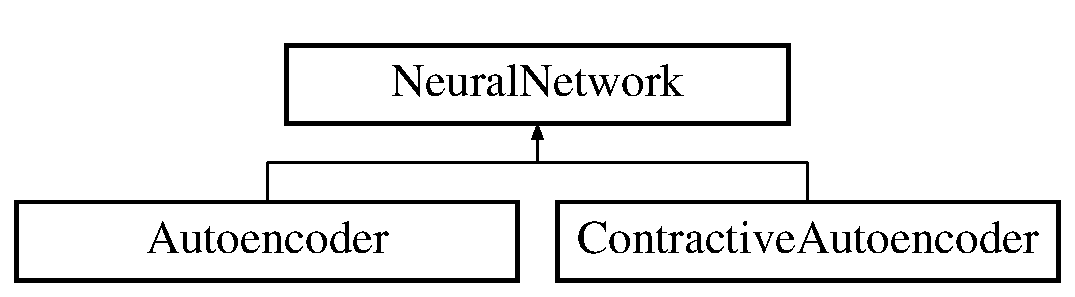
\includegraphics[height=2.000000cm]{classNeuralNetwork}
\end{center}
\end{figure}
\subsection*{Public Member Functions}
\begin{DoxyCompactItemize}
\item 
\hyperlink{classNeuralNetwork_accce4a7728e89a009a9d4ca1758c9b9d}{Neural\+Network} ()
\item 
double \hyperlink{classNeuralNetwork_a3c92371fb8eb9363460223b67f2716f4}{get\+L\+S\+Error} (double target, double predicted, int dist\+From\+Center)
\item 
int \hyperlink{classNeuralNetwork_a30196e8390fead450b9495b3a782b198}{make\+Weight\+Cpy} ()
\begin{DoxyCompactList}\small\item\em A function called when local minimum in the validation error is achieved, to store the combination of weights. \end{DoxyCompactList}\item 
double \hyperlink{classNeuralNetwork_a49f0a71b2cfd1bd2a4af986354fa103c}{delta\+Compute} (int mb)
\item 
double \hyperlink{classNeuralNetwork_aff3f167f69f75a74ce3c425b8783d321}{delta\+Compute\+Node\+Parallel} (int mb)
\item 
int \hyperlink{classNeuralNetwork_ae3d909ef30a5c179a236571e126aa841}{feedforward} (int mb)
\item 
int \hyperlink{classNeuralNetwork_aad8fc497e54c397d3e4e91376e02e939}{feedforward\+Node\+Parallel} (int mb)
\item 
int \hyperlink{classNeuralNetwork_a82af0b25c1099ac3818a36911b63e8db}{feedforward\+Node\+Parallel\+Comp\+Sparse} (int mb)
\item 
double \hyperlink{classNeuralNetwork_a9d80cfaedb341a1a94e5b932665904d4}{back\+PropagateU} (int mb, int la, int ii)
\item 
void \hyperlink{classNeuralNetwork_ab72a0bebc4933c5e495636fe15d33982}{initialise} (\hyperlink{classParamsInit}{Params\+Init} parameters)
\item 
void \hyperlink{classNeuralNetwork_a4e078c8f704a0118f9ed9457b5e6c74d}{initialise\+Drop\+Out} ()
\begin{DoxyCompactList}\small\item\em A function to initialise the vectors holding positions of the nodes to be set to 0. \end{DoxyCompactList}\item 
void \hyperlink{classNeuralNetwork_ae27621b39d0afef732ca36e5ab0a6b73}{initialise\+Stats\+Hidden\+Units} ()
\begin{DoxyCompactList}\small\item\em Allocate memory for the array holding the statistics about hidden units. \end{DoxyCompactList}\item 
void \hyperlink{classNeuralNetwork_a36525085d71d9aa8d755e5e19ebae7cc}{initialise\+Weights} (\hyperlink{classParamsInit}{Params\+Init} parameters)
\item 
void \hyperlink{classNeuralNetwork_ae8bd77cbaa88df5152db8a745254141c}{initialise\+Delta\+Bias} (\hyperlink{classParamsInit}{Params\+Init} parameters)
\item 
void \hyperlink{classNeuralNetwork_a77e3c1107530a1cb28021c7c2864c81f}{init\+Weights\+From\+File} (std\+::string path)
\item 
double \hyperlink{classNeuralNetwork_af0c6f4203d6c3b823a575954102bdf5d}{get\+Grad} (int kk, int jj, int ii)
\item 
double \hyperlink{classNeuralNetwork_adca7f84b7b063acebef819bae1abbaf7}{dot\+Product} (int mb, int kk, int jj)
\item 
void \hyperlink{classNeuralNetwork_af8a0997a14c97e1fb6ef97d3c132f808}{dot\+Product\+Prop} (int mb, int kk, int jj)
\item 
void \hyperlink{classNeuralNetwork_ad5d0e3d069c7ce2fbde30161771ba507}{set\+Layer\+U\+Output} (int mb, int la, int u, double val)
\item 
int \hyperlink{classNeuralNetwork_a1d0b90f44982811b3e28e3b9a4dfa810}{set\+Drop\+Out} ()
\begin{DoxyCompactList}\small\item\em A function to set the values of the drop out (shuffle the vectors) \end{DoxyCompactList}\item 
void \hyperlink{classNeuralNetwork_a2a84fe4a996154130853f031c6e475aa}{set\+Layer\+U\+Delta} (int mb, int la, int u, double val)
\item 
void \hyperlink{classNeuralNetwork_aeccccbe1b61dec7e4e76bd55bad7e591}{swap\+Weights} ()
\begin{DoxyCompactList}\small\item\em A function to swap the weights (current with the save with which the local minimum in the error is obtained) \end{DoxyCompactList}\item 
void \hyperlink{classNeuralNetwork_ad70d1e2802185f0126f0c52ac2dc55f1}{set\+Time\+Step} (int step)
\begin{DoxyCompactList}\small\item\em The function to set timestep. \end{DoxyCompactList}\item 
virtual int \hyperlink{classNeuralNetwork_acd83d73dbae85f80c1173bdb53e37726}{update\+Weights} (int ii, int jj, int kk, double val, double penalty)=0
\begin{DoxyCompactList}\small\item\em A virtual function implemented by C\+AE and AE to w = w-\/lr$\ast$grad with momentum and ada\+Grad. \end{DoxyCompactList}\item 
virtual int \hyperlink{classNeuralNetwork_a1bc1c063c3048b0551ae92352b553060}{update\+Weights\+Fast} (int ii, int jj, int kk, double val, double penalty)=0
\begin{DoxyCompactList}\small\item\em A virtual function implemented by C\+AE and AE to w = w-\/lr$\ast$grad without momentum and ada\+Grad. \end{DoxyCompactList}\item 
virtual int \hyperlink{classNeuralNetwork_af21bec3f1affe1a95346a57fd332f734}{backpropagate} (double learning\+Rate, double lambda)=0
\begin{DoxyCompactList}\small\item\em A virtual function implemented by C\+AE and AE to compute the backpropagation. \end{DoxyCompactList}\item 
virtual int \hyperlink{classNeuralNetwork_a01f72adec49e446ad4305bd6ad9859da}{backpropagate\+Node\+Parallel} (double learning\+Rate, double lambda, int flag\+Release)=0
\begin{DoxyCompactList}\small\item\em A virtual function implemented by C\+AE and AE to compute the backpropagation in parallel. \end{DoxyCompactList}\item 
virtual \hyperlink{classNeuralNetwork_a65475a7d7b05d302392333302626b2f8}{$\sim$\+Neural\+Network} ()
\begin{DoxyCompactList}\small\item\em A virtual destructor. \end{DoxyCompactList}\item 
virtual std\+::string \hyperlink{classNeuralNetwork_aa3edc74bdbc4d8730c0fcc935dad2af0}{type} () const  =0
\begin{DoxyCompactList}\small\item\em A virtual function giving the type of the encder (string) \end{DoxyCompactList}\item 
\hyperlink{classLayer}{Layer} $\ast$ \hyperlink{classNeuralNetwork_a6e03934244dc6512a2d7a481cce51ffc}{get\+Layer} (int mb, int id) const 
\item 
int \hyperlink{classNeuralNetwork_a715c7cc10103a070b270c44b25924608}{get\+Numb\+Layers} () const 
\item 
int \hyperlink{classNeuralNetwork_aa264beacf67eeeb94a869647c07c692b}{get\+Mini\+Batch} () const 
\item 
double \hyperlink{classNeuralNetwork_a3182abfff4d633ac07cdfb35f32169ae}{get\+Layer\+U\+Delta} (int mb, int la, int u) const 
\item 
int \hyperlink{classNeuralNetwork_a516fbda3ce38841218d09bb823c17994}{get\+Layer\+NumbU} (int la) const 
\item 
double \hyperlink{classNeuralNetwork_ae61ce4f7b97b61398b0087afe6ac6d82}{get\+Layer\+U\+Output} (int mb, int la, int u) const 
\item 
float \hyperlink{classNeuralNetwork_a837e0348677eee2872de3f78de404870}{get\+Stats} (int ii, int jj) const 
\item 
int \hyperlink{classNeuralNetwork_ad9fccddee1743c2428bcc3e8bc3e29ae}{get\+Layer\+Act} (int mb, int la) const 
\item 
double \hyperlink{classNeuralNetwork_a660717474efe687f8b7b4bfadd643fee}{get\+WeightO} (int ii, int jj, int kk) const 
\item 
double \hyperlink{classNeuralNetwork_a73d05958b2b8a1f8c4ffb7a82509928f}{get\+Momentum} () const 
\item 
double \hyperlink{classNeuralNetwork_a92237c8f168045e56c6d3953d56dcc51}{get\+Drop\+Out} () const 
\item 
double \hyperlink{classNeuralNetwork_a5eaca7be1f8654a7bcd0ff8bdbd8dcfa}{get\+Ada\+Grad} () const 
\item 
int \hyperlink{classNeuralNetwork_adeafd6db805901beaad9930dda8c904b}{get\+Stats\+Flag} () const 
\item 
bool \hyperlink{classNeuralNetwork_a81f82e65356f4698fe412f7a2f6203da}{get\+Swapped} () const 
\end{DoxyCompactItemize}
\subsection*{Protected Types}
\begin{DoxyCompactItemize}
\item 
enum \hyperlink{classNeuralNetwork_a4c1c6e488b842002a6d327726ff92dc5}{Flag} \{ \hyperlink{classNeuralNetwork_a4c1c6e488b842002a6d327726ff92dc5a0a2addaf6a0e180369ecaecb25f84d64}{disabled}, 
\hyperlink{classNeuralNetwork_a4c1c6e488b842002a6d327726ff92dc5ab40dedbb237d7d5e7aeef947a8f1cbc6}{enabled}
 \}\begin{DoxyCompactList}\small\item\em Flag to hold activated and deactivated values. \end{DoxyCompactList}
\end{DoxyCompactItemize}
\subsection*{Protected Attributes}
\begin{DoxyCompactItemize}
\item 
\hyperlink{classNeuralNetwork_a4c1c6e488b842002a6d327726ff92dc5}{Flag} \hyperlink{classNeuralNetwork_af7766960680b9a413ee4b36acad1e83d}{m\+\_\+flag\+Fast}
\begin{DoxyCompactList}\small\item\em Flag used to mark whether fast versions of the functions can be used. \end{DoxyCompactList}\item 
\hyperlink{classNeuralNetwork_a4c1c6e488b842002a6d327726ff92dc5}{Flag} \hyperlink{classNeuralNetwork_accd035b1b93fd424025aeb4b40a31394}{m\+\_\+stats\+Flag}
\begin{DoxyCompactList}\small\item\em Flag to mark whether the user wants to gather statistics. \end{DoxyCompactList}\item 
bool \hyperlink{classNeuralNetwork_a5009762781007f09860915f307701a60}{m\+\_\+flag\+Swapped}
\begin{DoxyCompactList}\small\item\em Flag to mark whether the weights have been swapped (i.\+e. local minimum reached) \end{DoxyCompactList}\item 
int \hyperlink{classNeuralNetwork_a1efaefc2c42a3d309c0b5e4a80a55f52}{m\+\_\+number\+Layers}
\begin{DoxyCompactList}\small\item\em Number of layers in the neural network. \end{DoxyCompactList}\item 
int \hyperlink{classNeuralNetwork_ad29fd15c4f0fc4c8fd214b4e815093b9}{m\+\_\+mini\+Batch}
\begin{DoxyCompactList}\small\item\em Mini-\/batch size. \end{DoxyCompactList}\item 
int \hyperlink{classNeuralNetwork_ae4f1fb12e7f5df8dac69abda6fe4d141}{m\+\_\+it\+Test}
\begin{DoxyCompactList}\small\item\em Number of test iterations. \end{DoxyCompactList}\item 
int \hyperlink{classNeuralNetwork_a25ea37c7b768bf2ade89c55b9e159ee2}{m\+\_\+it\+Train}
\begin{DoxyCompactList}\small\item\em Number of train iterations. \end{DoxyCompactList}\item 
int \hyperlink{classNeuralNetwork_aea6b9756c3ef7e82b2d40414beb37984}{m\+\_\+time\+Step}
\begin{DoxyCompactList}\small\item\em Time step. \end{DoxyCompactList}\item 
float \hyperlink{classNeuralNetwork_a30141464584fc2cc51599ffec4ce8dd8}{m\+\_\+ada\+Grad}
\begin{DoxyCompactList}\small\item\em Magnitude of the adaptive gradient \mbox{[}0;1) \end{DoxyCompactList}\item 
float \hyperlink{classNeuralNetwork_a8940dc6859b38907717cfec54e0929b1}{m\+\_\+momentum}
\begin{DoxyCompactList}\small\item\em Magnitude of the momentum \mbox{[}0;1) \end{DoxyCompactList}\item 
float \hyperlink{classNeuralNetwork_a754d963a6f58aee1e253f64d266ab487}{m\+\_\+drop\+Out}
\begin{DoxyCompactList}\small\item\em Fraction of the units set to 0. \end{DoxyCompactList}\item 
double \hyperlink{classNeuralNetwork_a5ff4dd9b7b90474cce090c37d7127366}{m\+\_\+sparse}
\begin{DoxyCompactList}\small\item\em Magnitude of the penalty. \end{DoxyCompactList}\item 
double \hyperlink{classNeuralNetwork_ac6e586b8ab49ef7ca1f07dab6f197f6c}{m\+\_\+sparsity\+Parameter}
\begin{DoxyCompactList}\small\item\em The maximum value of the output neurons expected. \end{DoxyCompactList}\item 
\hyperlink{classObjective}{Objective} \hyperlink{classNeuralNetwork_a296fef6f667d2bcf1080a16c8c3aceb2}{m\+\_\+objective}
\begin{DoxyCompactList}\small\item\em Variable to hold objective function. \end{DoxyCompactList}\item 
vector$<$ vector$<$ \hyperlink{classLayer}{Layer} $\ast$ $>$ $>$ \hyperlink{classNeuralNetwork_ab2bc4d407ef6b85a0089aaaa600e0fb8}{m\+\_\+layers}
\begin{DoxyCompactList}\small\item\em Matrix of layers (1D -\/ minibatch, 2D -\/ layers) \end{DoxyCompactList}\item 
vector$<$ int $>$ \hyperlink{classNeuralNetwork_a91b00cd0bb975be91e76eb13ffcfe78f}{m\+\_\+layers\+Size\+Vec}
\begin{DoxyCompactList}\small\item\em Vector to hold the sizes of layers. \end{DoxyCompactList}\item 
vector$<$ vector$<$ float $>$ $>$ \hyperlink{classNeuralNetwork_a15f7c03ca694dadc97a4290711ca2101}{m\+\_\+stats\+Hidden\+Units}
\begin{DoxyCompactList}\small\item\em Matrix to hold the stats about output of the hidden units. \end{DoxyCompactList}\item 
vector$<$ double $>$ \hyperlink{classNeuralNetwork_a257969584b79a83070b07462b1ec7fb2}{m\+\_\+av\+Units}
\begin{DoxyCompactList}\small\item\em Vector to hold regularization for the sparse autoencoder. \end{DoxyCompactList}\item 
vector$<$ double $>$ \hyperlink{classNeuralNetwork_ac447314a2315cd10f63b0b330857024a}{m\+\_\+sum\+Delta}
\begin{DoxyCompactList}\small\item\em Vector used for Open\+MP to store calculations produced by different threads. \end{DoxyCompactList}\item 
vector$<$ vector$<$ double $>$ $>$ \hyperlink{classNeuralNetwork_a456d6c273c0bd4f160f4d20f8b26f37b}{m\+\_\+drop\+Out\+Vec}
\begin{DoxyCompactList}\small\item\em Vector with elements 1 and 0 marking the neurons set to 0. \end{DoxyCompactList}\item 
vector$<$ vector$<$ vector$<$ double $>$ $>$ $>$ \hyperlink{classNeuralNetwork_ad489169464f3a6e827e6fb5de4419061}{m\+\_\+weights}
\begin{DoxyCompactList}\small\item\em Cube of weights. \end{DoxyCompactList}\item 
vector$<$ vector$<$ vector$<$ double $>$ $>$ $>$ \hyperlink{classNeuralNetwork_a9ac6bc441d6e2bfe7521d0b23ac8efdb}{m\+\_\+weights\+Min\+Cp}
\begin{DoxyCompactList}\small\item\em Cube of weights with which local minimum is achieved. \end{DoxyCompactList}\item 
vector$<$ vector$<$ vector$<$ double $>$ $>$ $>$ \hyperlink{classNeuralNetwork_a4345c084a3e1f604a3757e3b1ae3ad54}{m\+\_\+momentum\+Arr}
\begin{DoxyCompactList}\small\item\em Holding momentum for each weight. \end{DoxyCompactList}\item 
vector$<$ vector$<$ vector$<$ double $>$ $>$ $>$ \hyperlink{classNeuralNetwork_a0b6c7ff6e00c4f91e684217be91b0a28}{m\+\_\+sum\+Delta\+Arr}
\begin{DoxyCompactList}\small\item\em Holding deltas for the ada\+Grad. \end{DoxyCompactList}\end{DoxyCompactItemize}


\subsection{Detailed Description}
A base class for Neural Network Algorithms. 

A base class for contractive autoencoder and simple autoencoder. 

Definition at line 27 of file Neural\+Network.\+h.



\subsection{Member Enumeration Documentation}
\index{Neural\+Network@{Neural\+Network}!Flag@{Flag}}
\index{Flag@{Flag}!Neural\+Network@{Neural\+Network}}
\subsubsection[{\texorpdfstring{Flag}{Flag}}]{\setlength{\rightskip}{0pt plus 5cm}enum {\bf Neural\+Network\+::\+Flag}\hspace{0.3cm}{\ttfamily [protected]}}\hypertarget{classNeuralNetwork_a4c1c6e488b842002a6d327726ff92dc5}{}\label{classNeuralNetwork_a4c1c6e488b842002a6d327726ff92dc5}


Flag to hold activated and deactivated values. 

\begin{Desc}
\item[Enumerator]\par
\begin{description}
\index{disabled@{disabled}!Neural\+Network@{Neural\+Network}}\index{Neural\+Network@{Neural\+Network}!disabled@{disabled}}\item[{\em 
disabled\hypertarget{classNeuralNetwork_a4c1c6e488b842002a6d327726ff92dc5a0a2addaf6a0e180369ecaecb25f84d64}{}\label{classNeuralNetwork_a4c1c6e488b842002a6d327726ff92dc5a0a2addaf6a0e180369ecaecb25f84d64}
}]\index{enabled@{enabled}!Neural\+Network@{Neural\+Network}}\index{Neural\+Network@{Neural\+Network}!enabled@{enabled}}\item[{\em 
enabled\hypertarget{classNeuralNetwork_a4c1c6e488b842002a6d327726ff92dc5ab40dedbb237d7d5e7aeef947a8f1cbc6}{}\label{classNeuralNetwork_a4c1c6e488b842002a6d327726ff92dc5ab40dedbb237d7d5e7aeef947a8f1cbc6}
}]\end{description}
\end{Desc}


Definition at line 32 of file Neural\+Network.\+h.



\subsection{Constructor \& Destructor Documentation}
\index{Neural\+Network@{Neural\+Network}!Neural\+Network@{Neural\+Network}}
\index{Neural\+Network@{Neural\+Network}!Neural\+Network@{Neural\+Network}}
\subsubsection[{\texorpdfstring{Neural\+Network()}{NeuralNetwork()}}]{\setlength{\rightskip}{0pt plus 5cm}Neural\+Network\+::\+Neural\+Network (
\begin{DoxyParamCaption}
{}
\end{DoxyParamCaption}
)}\hypertarget{classNeuralNetwork_accce4a7728e89a009a9d4ca1758c9b9d}{}\label{classNeuralNetwork_accce4a7728e89a009a9d4ca1758c9b9d}


Definition at line 3 of file neuralnetwork.\+cpp.

\index{Neural\+Network@{Neural\+Network}!````~Neural\+Network@{$\sim$\+Neural\+Network}}
\index{````~Neural\+Network@{$\sim$\+Neural\+Network}!Neural\+Network@{Neural\+Network}}
\subsubsection[{\texorpdfstring{$\sim$\+Neural\+Network()}{~NeuralNetwork()}}]{\setlength{\rightskip}{0pt plus 5cm}Neural\+Network\+::$\sim$\+Neural\+Network (
\begin{DoxyParamCaption}
{}
\end{DoxyParamCaption}
)\hspace{0.3cm}{\ttfamily [virtual]}}\hypertarget{classNeuralNetwork_a65475a7d7b05d302392333302626b2f8}{}\label{classNeuralNetwork_a65475a7d7b05d302392333302626b2f8}


A virtual destructor. 



Definition at line 476 of file neuralnetwork.\+cpp.



\subsection{Member Function Documentation}
\index{Neural\+Network@{Neural\+Network}!backpropagate@{backpropagate}}
\index{backpropagate@{backpropagate}!Neural\+Network@{Neural\+Network}}
\subsubsection[{\texorpdfstring{backpropagate(double learning\+Rate, double lambda)=0}{backpropagate(double learningRate, double lambda)=0}}]{\setlength{\rightskip}{0pt plus 5cm}virtual int Neural\+Network\+::backpropagate (
\begin{DoxyParamCaption}
\item[{double}]{learning\+Rate, }
\item[{double}]{lambda}
\end{DoxyParamCaption}
)\hspace{0.3cm}{\ttfamily [pure virtual]}}\hypertarget{classNeuralNetwork_af21bec3f1affe1a95346a57fd332f734}{}\label{classNeuralNetwork_af21bec3f1affe1a95346a57fd332f734}


A virtual function implemented by C\+AE and AE to compute the backpropagation. 



Implemented in \hyperlink{classAutoencoder_a1a52083d0822fec947b93edf0797880f}{Autoencoder}, and \hyperlink{classContractiveAutoencoder_a66bf959d85d09b2f5cc2e06d6bdfe6bf}{Contractive\+Autoencoder}.

\index{Neural\+Network@{Neural\+Network}!backpropagate\+Node\+Parallel@{backpropagate\+Node\+Parallel}}
\index{backpropagate\+Node\+Parallel@{backpropagate\+Node\+Parallel}!Neural\+Network@{Neural\+Network}}
\subsubsection[{\texorpdfstring{backpropagate\+Node\+Parallel(double learning\+Rate, double lambda, int flag\+Release)=0}{backpropagateNodeParallel(double learningRate, double lambda, int flagRelease)=0}}]{\setlength{\rightskip}{0pt plus 5cm}virtual int Neural\+Network\+::backpropagate\+Node\+Parallel (
\begin{DoxyParamCaption}
\item[{double}]{learning\+Rate, }
\item[{double}]{lambda, }
\item[{int}]{flag\+Release}
\end{DoxyParamCaption}
)\hspace{0.3cm}{\ttfamily [pure virtual]}}\hypertarget{classNeuralNetwork_a01f72adec49e446ad4305bd6ad9859da}{}\label{classNeuralNetwork_a01f72adec49e446ad4305bd6ad9859da}


A virtual function implemented by C\+AE and AE to compute the backpropagation in parallel. 



Implemented in \hyperlink{classAutoencoder_aa5832a7ff94e5af13d6fa41489796d82}{Autoencoder}, and \hyperlink{classContractiveAutoencoder_a65daf5136737423ee6b0fd89442cbf70}{Contractive\+Autoencoder}.

\index{Neural\+Network@{Neural\+Network}!back\+PropagateU@{back\+PropagateU}}
\index{back\+PropagateU@{back\+PropagateU}!Neural\+Network@{Neural\+Network}}
\subsubsection[{\texorpdfstring{back\+Propagate\+U(int mb, int la, int ii)}{backPropagateU(int mb, int la, int ii)}}]{\setlength{\rightskip}{0pt plus 5cm}double Neural\+Network\+::back\+PropagateU (
\begin{DoxyParamCaption}
\item[{int}]{mb, }
\item[{int}]{la, }
\item[{int}]{ii}
\end{DoxyParamCaption}
)}\hypertarget{classNeuralNetwork_a9d80cfaedb341a1a94e5b932665904d4}{}\label{classNeuralNetwork_a9d80cfaedb341a1a94e5b932665904d4}
A function to apply the derivative of the non-\/linearity and get the propagated value 
\begin{DoxyParams}{Parameters}
{\em mb} & mini-\/batch \\
\hline
{\em la} & layer \\
\hline
{\em ii} & unit in the layer \\
\hline
\end{DoxyParams}


Definition at line 251 of file neuralnetwork.\+cpp.

\index{Neural\+Network@{Neural\+Network}!delta\+Compute@{delta\+Compute}}
\index{delta\+Compute@{delta\+Compute}!Neural\+Network@{Neural\+Network}}
\subsubsection[{\texorpdfstring{delta\+Compute(int mb)}{deltaCompute(int mb)}}]{\setlength{\rightskip}{0pt plus 5cm}double Neural\+Network\+::delta\+Compute (
\begin{DoxyParamCaption}
\item[{int}]{mb}
\end{DoxyParamCaption}
)}\hypertarget{classNeuralNetwork_a49f0a71b2cfd1bd2a4af986354fa103c}{}\label{classNeuralNetwork_a49f0a71b2cfd1bd2a4af986354fa103c}
A function to compute deltas for a given mini-\/batch 
\begin{DoxyParams}{Parameters}
{\em mb} & mini-\/batch \\
\hline
\end{DoxyParams}


Definition at line 212 of file neuralnetwork.\+cpp.

\index{Neural\+Network@{Neural\+Network}!delta\+Compute\+Node\+Parallel@{delta\+Compute\+Node\+Parallel}}
\index{delta\+Compute\+Node\+Parallel@{delta\+Compute\+Node\+Parallel}!Neural\+Network@{Neural\+Network}}
\subsubsection[{\texorpdfstring{delta\+Compute\+Node\+Parallel(int mb)}{deltaComputeNodeParallel(int mb)}}]{\setlength{\rightskip}{0pt plus 5cm}double Neural\+Network\+::delta\+Compute\+Node\+Parallel (
\begin{DoxyParamCaption}
\item[{int}]{mb}
\end{DoxyParamCaption}
)}\hypertarget{classNeuralNetwork_aff3f167f69f75a74ce3c425b8783d321}{}\label{classNeuralNetwork_aff3f167f69f75a74ce3c425b8783d321}
A parallel function to compute deltas for a given mini-\/batch 
\begin{DoxyParams}{Parameters}
{\em mb} & mini-\/batch \\
\hline
\end{DoxyParams}
m\+\_\+av\+Units\mbox{[}jj\mbox{]}=0.\+0; Y\+OU C\+A\+N\+N\+OT 0, beacuse the value is used in the next iteration 

Definition at line 133 of file neuralnetwork.\+cpp.

\index{Neural\+Network@{Neural\+Network}!dot\+Product@{dot\+Product}}
\index{dot\+Product@{dot\+Product}!Neural\+Network@{Neural\+Network}}
\subsubsection[{\texorpdfstring{dot\+Product(int mb, int kk, int jj)}{dotProduct(int mb, int kk, int jj)}}]{\setlength{\rightskip}{0pt plus 5cm}double Neural\+Network\+::dot\+Product (
\begin{DoxyParamCaption}
\item[{int}]{mb, }
\item[{int}]{kk, }
\item[{int}]{jj}
\end{DoxyParamCaption}
)}\hypertarget{classNeuralNetwork_adca7f84b7b063acebef819bae1abbaf7}{}\label{classNeuralNetwork_adca7f84b7b063acebef819bae1abbaf7}
A function 
\begin{DoxyParams}{Parameters}
{\em mb} & \\
\hline
{\em kk} & \\
\hline
{\em jj} & \\
\hline
\end{DoxyParams}


Definition at line 111 of file neuralnetwork.\+cpp.

\index{Neural\+Network@{Neural\+Network}!dot\+Product\+Prop@{dot\+Product\+Prop}}
\index{dot\+Product\+Prop@{dot\+Product\+Prop}!Neural\+Network@{Neural\+Network}}
\subsubsection[{\texorpdfstring{dot\+Product\+Prop(int mb, int kk, int jj)}{dotProductProp(int mb, int kk, int jj)}}]{\setlength{\rightskip}{0pt plus 5cm}void Neural\+Network\+::dot\+Product\+Prop (
\begin{DoxyParamCaption}
\item[{int}]{mb, }
\item[{int}]{kk, }
\item[{int}]{jj}
\end{DoxyParamCaption}
)}\hypertarget{classNeuralNetwork_af8a0997a14c97e1fb6ef97d3c132f808}{}\label{classNeuralNetwork_af8a0997a14c97e1fb6ef97d3c132f808}
A function called from the feedforward to compute the dot product of the neuron outputs with associated weights and pass it through the non-\/linearity 
\begin{DoxyParams}{Parameters}
{\em mb} & \\
\hline
{\em kk} & \\
\hline
{\em jj} & \\
\hline
\end{DoxyParams}


Definition at line 124 of file neuralnetwork.\+cpp.

\index{Neural\+Network@{Neural\+Network}!feedforward@{feedforward}}
\index{feedforward@{feedforward}!Neural\+Network@{Neural\+Network}}
\subsubsection[{\texorpdfstring{feedforward(int mb)}{feedforward(int mb)}}]{\setlength{\rightskip}{0pt plus 5cm}int Neural\+Network\+::feedforward (
\begin{DoxyParamCaption}
\item[{int}]{mb}
\end{DoxyParamCaption}
)}\hypertarget{classNeuralNetwork_ae3d909ef30a5c179a236571e126aa841}{}\label{classNeuralNetwork_ae3d909ef30a5c179a236571e126aa841}
Feedforward 
\begin{DoxyParams}{Parameters}
{\em mb} & -\/ mini-\/batch \\
\hline
\end{DoxyParams}


Definition at line 49 of file neuralnetwork.\+cpp.

\index{Neural\+Network@{Neural\+Network}!feedforward\+Node\+Parallel@{feedforward\+Node\+Parallel}}
\index{feedforward\+Node\+Parallel@{feedforward\+Node\+Parallel}!Neural\+Network@{Neural\+Network}}
\subsubsection[{\texorpdfstring{feedforward\+Node\+Parallel(int mb)}{feedforwardNodeParallel(int mb)}}]{\setlength{\rightskip}{0pt plus 5cm}int Neural\+Network\+::feedforward\+Node\+Parallel (
\begin{DoxyParamCaption}
\item[{int}]{mb}
\end{DoxyParamCaption}
)}\hypertarget{classNeuralNetwork_aad8fc497e54c397d3e4e91376e02e939}{}\label{classNeuralNetwork_aad8fc497e54c397d3e4e91376e02e939}
Node parallel feedforward 
\begin{DoxyParams}{Parameters}
{\em mb} & -\/ mini-\/batch \\
\hline
\end{DoxyParams}


Definition at line 93 of file neuralnetwork.\+cpp.

\index{Neural\+Network@{Neural\+Network}!feedforward\+Node\+Parallel\+Comp\+Sparse@{feedforward\+Node\+Parallel\+Comp\+Sparse}}
\index{feedforward\+Node\+Parallel\+Comp\+Sparse@{feedforward\+Node\+Parallel\+Comp\+Sparse}!Neural\+Network@{Neural\+Network}}
\subsubsection[{\texorpdfstring{feedforward\+Node\+Parallel\+Comp\+Sparse(int mb)}{feedforwardNodeParallelCompSparse(int mb)}}]{\setlength{\rightskip}{0pt plus 5cm}int Neural\+Network\+::feedforward\+Node\+Parallel\+Comp\+Sparse (
\begin{DoxyParamCaption}
\item[{int}]{mb}
\end{DoxyParamCaption}
)}\hypertarget{classNeuralNetwork_a82af0b25c1099ac3818a36911b63e8db}{}\label{classNeuralNetwork_a82af0b25c1099ac3818a36911b63e8db}
A feed forward function used to compute the penalty for the sparse autoencoder 
\begin{DoxyParams}{Parameters}
{\em mb} & mini-\/batch \\
\hline
\end{DoxyParams}


Definition at line 72 of file neuralnetwork.\+cpp.

\index{Neural\+Network@{Neural\+Network}!get\+Ada\+Grad@{get\+Ada\+Grad}}
\index{get\+Ada\+Grad@{get\+Ada\+Grad}!Neural\+Network@{Neural\+Network}}
\subsubsection[{\texorpdfstring{get\+Ada\+Grad() const }{getAdaGrad() const }}]{\setlength{\rightskip}{0pt plus 5cm}double Neural\+Network\+::get\+Ada\+Grad (
\begin{DoxyParamCaption}
{}
\end{DoxyParamCaption}
) const\hspace{0.3cm}{\ttfamily [inline]}}\hypertarget{classNeuralNetwork_a5eaca7be1f8654a7bcd0ff8bdbd8dcfa}{}\label{classNeuralNetwork_a5eaca7be1f8654a7bcd0ff8bdbd8dcfa}


Definition at line 252 of file Neural\+Network.\+h.

\index{Neural\+Network@{Neural\+Network}!get\+Drop\+Out@{get\+Drop\+Out}}
\index{get\+Drop\+Out@{get\+Drop\+Out}!Neural\+Network@{Neural\+Network}}
\subsubsection[{\texorpdfstring{get\+Drop\+Out() const }{getDropOut() const }}]{\setlength{\rightskip}{0pt plus 5cm}double Neural\+Network\+::get\+Drop\+Out (
\begin{DoxyParamCaption}
{}
\end{DoxyParamCaption}
) const\hspace{0.3cm}{\ttfamily [inline]}}\hypertarget{classNeuralNetwork_a92237c8f168045e56c6d3953d56dcc51}{}\label{classNeuralNetwork_a92237c8f168045e56c6d3953d56dcc51}


Definition at line 250 of file Neural\+Network.\+h.

\index{Neural\+Network@{Neural\+Network}!get\+Grad@{get\+Grad}}
\index{get\+Grad@{get\+Grad}!Neural\+Network@{Neural\+Network}}
\subsubsection[{\texorpdfstring{get\+Grad(int kk, int jj, int ii)}{getGrad(int kk, int jj, int ii)}}]{\setlength{\rightskip}{0pt plus 5cm}double Neural\+Network\+::get\+Grad (
\begin{DoxyParamCaption}
\item[{int}]{kk, }
\item[{int}]{jj, }
\item[{int}]{ii}
\end{DoxyParamCaption}
)}\hypertarget{classNeuralNetwork_af0c6f4203d6c3b823a575954102bdf5d}{}\label{classNeuralNetwork_af0c6f4203d6c3b823a575954102bdf5d}
A function used to get the gradient in the backporapagation stage 
\begin{DoxyParams}{Parameters}
{\em kk} & -\/ layer \\
\hline
{\em jj} & -\/ unit in the kk layer \\
\hline
{\em ii} & -\/ unit in the (kk-\/1) layer \\
\hline
\end{DoxyParams}


Definition at line 256 of file neuralnetwork.\+cpp.

\index{Neural\+Network@{Neural\+Network}!get\+Layer@{get\+Layer}}
\index{get\+Layer@{get\+Layer}!Neural\+Network@{Neural\+Network}}
\subsubsection[{\texorpdfstring{get\+Layer(int mb, int id) const }{getLayer(int mb, int id) const }}]{\setlength{\rightskip}{0pt plus 5cm}{\bf Layer}$\ast$ Neural\+Network\+::get\+Layer (
\begin{DoxyParamCaption}
\item[{int}]{mb, }
\item[{int}]{id}
\end{DoxyParamCaption}
) const\hspace{0.3cm}{\ttfamily [inline]}}\hypertarget{classNeuralNetwork_a6e03934244dc6512a2d7a481cce51ffc}{}\label{classNeuralNetwork_a6e03934244dc6512a2d7a481cce51ffc}


Definition at line 230 of file Neural\+Network.\+h.

\index{Neural\+Network@{Neural\+Network}!get\+Layer\+Act@{get\+Layer\+Act}}
\index{get\+Layer\+Act@{get\+Layer\+Act}!Neural\+Network@{Neural\+Network}}
\subsubsection[{\texorpdfstring{get\+Layer\+Act(int mb, int la) const }{getLayerAct(int mb, int la) const }}]{\setlength{\rightskip}{0pt plus 5cm}int Neural\+Network\+::get\+Layer\+Act (
\begin{DoxyParamCaption}
\item[{int}]{mb, }
\item[{int}]{la}
\end{DoxyParamCaption}
) const\hspace{0.3cm}{\ttfamily [inline]}}\hypertarget{classNeuralNetwork_ad9fccddee1743c2428bcc3e8bc3e29ae}{}\label{classNeuralNetwork_ad9fccddee1743c2428bcc3e8bc3e29ae}


Definition at line 244 of file Neural\+Network.\+h.

\index{Neural\+Network@{Neural\+Network}!get\+Layer\+NumbU@{get\+Layer\+NumbU}}
\index{get\+Layer\+NumbU@{get\+Layer\+NumbU}!Neural\+Network@{Neural\+Network}}
\subsubsection[{\texorpdfstring{get\+Layer\+Numb\+U(int la) const }{getLayerNumbU(int la) const }}]{\setlength{\rightskip}{0pt plus 5cm}int Neural\+Network\+::get\+Layer\+NumbU (
\begin{DoxyParamCaption}
\item[{int}]{la}
\end{DoxyParamCaption}
) const\hspace{0.3cm}{\ttfamily [inline]}}\hypertarget{classNeuralNetwork_a516fbda3ce38841218d09bb823c17994}{}\label{classNeuralNetwork_a516fbda3ce38841218d09bb823c17994}


Definition at line 238 of file Neural\+Network.\+h.

\index{Neural\+Network@{Neural\+Network}!get\+Layer\+U\+Delta@{get\+Layer\+U\+Delta}}
\index{get\+Layer\+U\+Delta@{get\+Layer\+U\+Delta}!Neural\+Network@{Neural\+Network}}
\subsubsection[{\texorpdfstring{get\+Layer\+U\+Delta(int mb, int la, int u) const }{getLayerUDelta(int mb, int la, int u) const }}]{\setlength{\rightskip}{0pt plus 5cm}double Neural\+Network\+::get\+Layer\+U\+Delta (
\begin{DoxyParamCaption}
\item[{int}]{mb, }
\item[{int}]{la, }
\item[{int}]{u}
\end{DoxyParamCaption}
) const\hspace{0.3cm}{\ttfamily [inline]}}\hypertarget{classNeuralNetwork_a3182abfff4d633ac07cdfb35f32169ae}{}\label{classNeuralNetwork_a3182abfff4d633ac07cdfb35f32169ae}


Definition at line 236 of file Neural\+Network.\+h.

\index{Neural\+Network@{Neural\+Network}!get\+Layer\+U\+Output@{get\+Layer\+U\+Output}}
\index{get\+Layer\+U\+Output@{get\+Layer\+U\+Output}!Neural\+Network@{Neural\+Network}}
\subsubsection[{\texorpdfstring{get\+Layer\+U\+Output(int mb, int la, int u) const }{getLayerUOutput(int mb, int la, int u) const }}]{\setlength{\rightskip}{0pt plus 5cm}double Neural\+Network\+::get\+Layer\+U\+Output (
\begin{DoxyParamCaption}
\item[{int}]{mb, }
\item[{int}]{la, }
\item[{int}]{u}
\end{DoxyParamCaption}
) const\hspace{0.3cm}{\ttfamily [inline]}}\hypertarget{classNeuralNetwork_ae61ce4f7b97b61398b0087afe6ac6d82}{}\label{classNeuralNetwork_ae61ce4f7b97b61398b0087afe6ac6d82}


Definition at line 240 of file Neural\+Network.\+h.

\index{Neural\+Network@{Neural\+Network}!get\+L\+S\+Error@{get\+L\+S\+Error}}
\index{get\+L\+S\+Error@{get\+L\+S\+Error}!Neural\+Network@{Neural\+Network}}
\subsubsection[{\texorpdfstring{get\+L\+S\+Error(double target, double predicted, int dist\+From\+Center)}{getLSError(double target, double predicted, int distFromCenter)}}]{\setlength{\rightskip}{0pt plus 5cm}double Neural\+Network\+::get\+L\+S\+Error (
\begin{DoxyParamCaption}
\item[{double}]{target, }
\item[{double}]{predicted, }
\item[{int}]{dist\+From\+Center}
\end{DoxyParamCaption}
)}\hypertarget{classNeuralNetwork_a3c92371fb8eb9363460223b67f2716f4}{}\label{classNeuralNetwork_a3c92371fb8eb9363460223b67f2716f4}
The function to get the Squared error between the target and predicted values used in to weight error on the edges of the patches 
\begin{DoxyParams}{Parameters}
{\em target} & -\/ target value \\
\hline
{\em predicted} & -\/ predicted value \\
\hline
{\em dist\+From\+Center} & -\/ distance of the point from the center of the patch \\
\hline
\end{DoxyParams}


Definition at line 8 of file neuralnetwork.\+cpp.

\index{Neural\+Network@{Neural\+Network}!get\+Mini\+Batch@{get\+Mini\+Batch}}
\index{get\+Mini\+Batch@{get\+Mini\+Batch}!Neural\+Network@{Neural\+Network}}
\subsubsection[{\texorpdfstring{get\+Mini\+Batch() const }{getMiniBatch() const }}]{\setlength{\rightskip}{0pt plus 5cm}int Neural\+Network\+::get\+Mini\+Batch (
\begin{DoxyParamCaption}
{}
\end{DoxyParamCaption}
) const\hspace{0.3cm}{\ttfamily [inline]}}\hypertarget{classNeuralNetwork_aa264beacf67eeeb94a869647c07c692b}{}\label{classNeuralNetwork_aa264beacf67eeeb94a869647c07c692b}


Definition at line 234 of file Neural\+Network.\+h.

\index{Neural\+Network@{Neural\+Network}!get\+Momentum@{get\+Momentum}}
\index{get\+Momentum@{get\+Momentum}!Neural\+Network@{Neural\+Network}}
\subsubsection[{\texorpdfstring{get\+Momentum() const }{getMomentum() const }}]{\setlength{\rightskip}{0pt plus 5cm}double Neural\+Network\+::get\+Momentum (
\begin{DoxyParamCaption}
{}
\end{DoxyParamCaption}
) const\hspace{0.3cm}{\ttfamily [inline]}}\hypertarget{classNeuralNetwork_a73d05958b2b8a1f8c4ffb7a82509928f}{}\label{classNeuralNetwork_a73d05958b2b8a1f8c4ffb7a82509928f}


Definition at line 248 of file Neural\+Network.\+h.

\index{Neural\+Network@{Neural\+Network}!get\+Numb\+Layers@{get\+Numb\+Layers}}
\index{get\+Numb\+Layers@{get\+Numb\+Layers}!Neural\+Network@{Neural\+Network}}
\subsubsection[{\texorpdfstring{get\+Numb\+Layers() const }{getNumbLayers() const }}]{\setlength{\rightskip}{0pt plus 5cm}int Neural\+Network\+::get\+Numb\+Layers (
\begin{DoxyParamCaption}
{}
\end{DoxyParamCaption}
) const\hspace{0.3cm}{\ttfamily [inline]}}\hypertarget{classNeuralNetwork_a715c7cc10103a070b270c44b25924608}{}\label{classNeuralNetwork_a715c7cc10103a070b270c44b25924608}


Definition at line 232 of file Neural\+Network.\+h.

\index{Neural\+Network@{Neural\+Network}!get\+Stats@{get\+Stats}}
\index{get\+Stats@{get\+Stats}!Neural\+Network@{Neural\+Network}}
\subsubsection[{\texorpdfstring{get\+Stats(int ii, int jj) const }{getStats(int ii, int jj) const }}]{\setlength{\rightskip}{0pt plus 5cm}float Neural\+Network\+::get\+Stats (
\begin{DoxyParamCaption}
\item[{int}]{ii, }
\item[{int}]{jj}
\end{DoxyParamCaption}
) const\hspace{0.3cm}{\ttfamily [inline]}}\hypertarget{classNeuralNetwork_a837e0348677eee2872de3f78de404870}{}\label{classNeuralNetwork_a837e0348677eee2872de3f78de404870}


Definition at line 242 of file Neural\+Network.\+h.

\index{Neural\+Network@{Neural\+Network}!get\+Stats\+Flag@{get\+Stats\+Flag}}
\index{get\+Stats\+Flag@{get\+Stats\+Flag}!Neural\+Network@{Neural\+Network}}
\subsubsection[{\texorpdfstring{get\+Stats\+Flag() const }{getStatsFlag() const }}]{\setlength{\rightskip}{0pt plus 5cm}int Neural\+Network\+::get\+Stats\+Flag (
\begin{DoxyParamCaption}
{}
\end{DoxyParamCaption}
) const\hspace{0.3cm}{\ttfamily [inline]}}\hypertarget{classNeuralNetwork_adeafd6db805901beaad9930dda8c904b}{}\label{classNeuralNetwork_adeafd6db805901beaad9930dda8c904b}


Definition at line 254 of file Neural\+Network.\+h.

\index{Neural\+Network@{Neural\+Network}!get\+Swapped@{get\+Swapped}}
\index{get\+Swapped@{get\+Swapped}!Neural\+Network@{Neural\+Network}}
\subsubsection[{\texorpdfstring{get\+Swapped() const }{getSwapped() const }}]{\setlength{\rightskip}{0pt plus 5cm}bool Neural\+Network\+::get\+Swapped (
\begin{DoxyParamCaption}
{}
\end{DoxyParamCaption}
) const\hspace{0.3cm}{\ttfamily [inline]}}\hypertarget{classNeuralNetwork_a81f82e65356f4698fe412f7a2f6203da}{}\label{classNeuralNetwork_a81f82e65356f4698fe412f7a2f6203da}


Definition at line 256 of file Neural\+Network.\+h.

\index{Neural\+Network@{Neural\+Network}!get\+WeightO@{get\+WeightO}}
\index{get\+WeightO@{get\+WeightO}!Neural\+Network@{Neural\+Network}}
\subsubsection[{\texorpdfstring{get\+Weight\+O(int ii, int jj, int kk) const }{getWeightO(int ii, int jj, int kk) const }}]{\setlength{\rightskip}{0pt plus 5cm}double Neural\+Network\+::get\+WeightO (
\begin{DoxyParamCaption}
\item[{int}]{ii, }
\item[{int}]{jj, }
\item[{int}]{kk}
\end{DoxyParamCaption}
) const\hspace{0.3cm}{\ttfamily [inline]}}\hypertarget{classNeuralNetwork_a660717474efe687f8b7b4bfadd643fee}{}\label{classNeuralNetwork_a660717474efe687f8b7b4bfadd643fee}


Definition at line 246 of file Neural\+Network.\+h.

\index{Neural\+Network@{Neural\+Network}!initialise@{initialise}}
\index{initialise@{initialise}!Neural\+Network@{Neural\+Network}}
\subsubsection[{\texorpdfstring{initialise(\+Params\+Init parameters)}{initialise(ParamsInit parameters)}}]{\setlength{\rightskip}{0pt plus 5cm}void Neural\+Network\+::initialise (
\begin{DoxyParamCaption}
\item[{{\bf Params\+Init}}]{parameters}
\end{DoxyParamCaption}
)}\hypertarget{classNeuralNetwork_ab72a0bebc4933c5e495636fe15d33982}{}\label{classNeuralNetwork_ab72a0bebc4933c5e495636fe15d33982}
A function to initialise the Neural netowrk 
\begin{DoxyParams}{Parameters}
{\em parameters} & used to stor contents of the config file \\
\hline
\end{DoxyParams}
Drop out initialise

Stats hidden units initialise

Bias set

Function to Initialise Weights 

Definition at line 276 of file neuralnetwork.\+cpp.

\index{Neural\+Network@{Neural\+Network}!initialise\+Delta\+Bias@{initialise\+Delta\+Bias}}
\index{initialise\+Delta\+Bias@{initialise\+Delta\+Bias}!Neural\+Network@{Neural\+Network}}
\subsubsection[{\texorpdfstring{initialise\+Delta\+Bias(\+Params\+Init parameters)}{initialiseDeltaBias(ParamsInit parameters)}}]{\setlength{\rightskip}{0pt plus 5cm}void Neural\+Network\+::initialise\+Delta\+Bias (
\begin{DoxyParamCaption}
\item[{{\bf Params\+Init}}]{parameters}
\end{DoxyParamCaption}
)}\hypertarget{classNeuralNetwork_ae8bd77cbaa88df5152db8a745254141c}{}\label{classNeuralNetwork_ae8bd77cbaa88df5152db8a745254141c}
A function to set bias and delta values 
\begin{DoxyParams}{Parameters}
{\em parameters} & -\/ used to stor the results from the config file \\
\hline
\end{DoxyParams}


Definition at line 327 of file neuralnetwork.\+cpp.

\index{Neural\+Network@{Neural\+Network}!initialise\+Drop\+Out@{initialise\+Drop\+Out}}
\index{initialise\+Drop\+Out@{initialise\+Drop\+Out}!Neural\+Network@{Neural\+Network}}
\subsubsection[{\texorpdfstring{initialise\+Drop\+Out()}{initialiseDropOut()}}]{\setlength{\rightskip}{0pt plus 5cm}void Neural\+Network\+::initialise\+Drop\+Out (
\begin{DoxyParamCaption}
{}
\end{DoxyParamCaption}
)}\hypertarget{classNeuralNetwork_a4e078c8f704a0118f9ed9457b5e6c74d}{}\label{classNeuralNetwork_a4e078c8f704a0118f9ed9457b5e6c74d}


A function to initialise the vectors holding positions of the nodes to be set to 0. 



Definition at line 344 of file neuralnetwork.\+cpp.

\index{Neural\+Network@{Neural\+Network}!initialise\+Stats\+Hidden\+Units@{initialise\+Stats\+Hidden\+Units}}
\index{initialise\+Stats\+Hidden\+Units@{initialise\+Stats\+Hidden\+Units}!Neural\+Network@{Neural\+Network}}
\subsubsection[{\texorpdfstring{initialise\+Stats\+Hidden\+Units()}{initialiseStatsHiddenUnits()}}]{\setlength{\rightskip}{0pt plus 5cm}void Neural\+Network\+::initialise\+Stats\+Hidden\+Units (
\begin{DoxyParamCaption}
{}
\end{DoxyParamCaption}
)}\hypertarget{classNeuralNetwork_ae27621b39d0afef732ca36e5ab0a6b73}{}\label{classNeuralNetwork_ae27621b39d0afef732ca36e5ab0a6b73}


Allocate memory for the array holding the statistics about hidden units. 



Definition at line 366 of file neuralnetwork.\+cpp.

\index{Neural\+Network@{Neural\+Network}!initialise\+Weights@{initialise\+Weights}}
\index{initialise\+Weights@{initialise\+Weights}!Neural\+Network@{Neural\+Network}}
\subsubsection[{\texorpdfstring{initialise\+Weights(\+Params\+Init parameters)}{initialiseWeights(ParamsInit parameters)}}]{\setlength{\rightskip}{0pt plus 5cm}void Neural\+Network\+::initialise\+Weights (
\begin{DoxyParamCaption}
\item[{{\bf Params\+Init}}]{parameters}
\end{DoxyParamCaption}
)}\hypertarget{classNeuralNetwork_a36525085d71d9aa8d755e5e19ebae7cc}{}\label{classNeuralNetwork_a36525085d71d9aa8d755e5e19ebae7cc}
A function to initialise weights 
\begin{DoxyParams}{Parameters}
{\em parameters} & -\/ used to stor the results from the config file \\
\hline
\end{DoxyParams}


Definition at line 382 of file neuralnetwork.\+cpp.

\index{Neural\+Network@{Neural\+Network}!init\+Weights\+From\+File@{init\+Weights\+From\+File}}
\index{init\+Weights\+From\+File@{init\+Weights\+From\+File}!Neural\+Network@{Neural\+Network}}
\subsubsection[{\texorpdfstring{init\+Weights\+From\+File(std\+::string path)}{initWeightsFromFile(std::string path)}}]{\setlength{\rightskip}{0pt plus 5cm}void Neural\+Network\+::init\+Weights\+From\+File (
\begin{DoxyParamCaption}
\item[{std\+::string}]{path}
\end{DoxyParamCaption}
)}\hypertarget{classNeuralNetwork_a77e3c1107530a1cb28021c7c2864c81f}{}\label{classNeuralNetwork_a77e3c1107530a1cb28021c7c2864c81f}
A function used to initialise weights from the file 
\begin{DoxyParams}{Parameters}
{\em path} & -\/ a path to the weights file \\
\hline
\end{DoxyParams}


Definition at line 431 of file neuralnetwork.\+cpp.

\index{Neural\+Network@{Neural\+Network}!make\+Weight\+Cpy@{make\+Weight\+Cpy}}
\index{make\+Weight\+Cpy@{make\+Weight\+Cpy}!Neural\+Network@{Neural\+Network}}
\subsubsection[{\texorpdfstring{make\+Weight\+Cpy()}{makeWeightCpy()}}]{\setlength{\rightskip}{0pt plus 5cm}int Neural\+Network\+::make\+Weight\+Cpy (
\begin{DoxyParamCaption}
{}
\end{DoxyParamCaption}
)}\hypertarget{classNeuralNetwork_a30196e8390fead450b9495b3a782b198}{}\label{classNeuralNetwork_a30196e8390fead450b9495b3a782b198}


A function called when local minimum in the validation error is achieved, to store the combination of weights. 



Definition at line 21 of file neuralnetwork.\+cpp.

\index{Neural\+Network@{Neural\+Network}!set\+Drop\+Out@{set\+Drop\+Out}}
\index{set\+Drop\+Out@{set\+Drop\+Out}!Neural\+Network@{Neural\+Network}}
\subsubsection[{\texorpdfstring{set\+Drop\+Out()}{setDropOut()}}]{\setlength{\rightskip}{0pt plus 5cm}int Neural\+Network\+::set\+Drop\+Out (
\begin{DoxyParamCaption}
{}
\end{DoxyParamCaption}
)}\hypertarget{classNeuralNetwork_a1d0b90f44982811b3e28e3b9a4dfa810}{}\label{classNeuralNetwork_a1d0b90f44982811b3e28e3b9a4dfa810}


A function to set the values of the drop out (shuffle the vectors) 



Definition at line 40 of file neuralnetwork.\+cpp.

\index{Neural\+Network@{Neural\+Network}!set\+Layer\+U\+Delta@{set\+Layer\+U\+Delta}}
\index{set\+Layer\+U\+Delta@{set\+Layer\+U\+Delta}!Neural\+Network@{Neural\+Network}}
\subsubsection[{\texorpdfstring{set\+Layer\+U\+Delta(int mb, int la, int u, double val)}{setLayerUDelta(int mb, int la, int u, double val)}}]{\setlength{\rightskip}{0pt plus 5cm}void Neural\+Network\+::set\+Layer\+U\+Delta (
\begin{DoxyParamCaption}
\item[{int}]{mb, }
\item[{int}]{la, }
\item[{int}]{u, }
\item[{double}]{val}
\end{DoxyParamCaption}
)}\hypertarget{classNeuralNetwork_a2a84fe4a996154130853f031c6e475aa}{}\label{classNeuralNetwork_a2a84fe4a996154130853f031c6e475aa}
A function to set the delta of the unit 
\begin{DoxyParams}{Parameters}
{\em mb} & -\/ mini-\/batch \\
\hline
{\em la} & -\/ layer \\
\hline
{\em u} & -\/ unit \\
\hline
{\em val} & -\/ value \\
\hline
\end{DoxyParams}


Definition at line 271 of file neuralnetwork.\+cpp.

\index{Neural\+Network@{Neural\+Network}!set\+Layer\+U\+Output@{set\+Layer\+U\+Output}}
\index{set\+Layer\+U\+Output@{set\+Layer\+U\+Output}!Neural\+Network@{Neural\+Network}}
\subsubsection[{\texorpdfstring{set\+Layer\+U\+Output(int mb, int la, int u, double val)}{setLayerUOutput(int mb, int la, int u, double val)}}]{\setlength{\rightskip}{0pt plus 5cm}void Neural\+Network\+::set\+Layer\+U\+Output (
\begin{DoxyParamCaption}
\item[{int}]{mb, }
\item[{int}]{la, }
\item[{int}]{u, }
\item[{double}]{val}
\end{DoxyParamCaption}
)}\hypertarget{classNeuralNetwork_ad5d0e3d069c7ce2fbde30161771ba507}{}\label{classNeuralNetwork_ad5d0e3d069c7ce2fbde30161771ba507}
A function to set the output of the unit 
\begin{DoxyParams}{Parameters}
{\em mb} & -\/ mini-\/batch \\
\hline
{\em la} & -\/ layer \\
\hline
{\em u} & -\/ unit \\
\hline
{\em val} & -\/ value \\
\hline
\end{DoxyParams}


Definition at line 267 of file neuralnetwork.\+cpp.

\index{Neural\+Network@{Neural\+Network}!set\+Time\+Step@{set\+Time\+Step}}
\index{set\+Time\+Step@{set\+Time\+Step}!Neural\+Network@{Neural\+Network}}
\subsubsection[{\texorpdfstring{set\+Time\+Step(int step)}{setTimeStep(int step)}}]{\setlength{\rightskip}{0pt plus 5cm}void Neural\+Network\+::set\+Time\+Step (
\begin{DoxyParamCaption}
\item[{int}]{step}
\end{DoxyParamCaption}
)\hspace{0.3cm}{\ttfamily [inline]}}\hypertarget{classNeuralNetwork_ad70d1e2802185f0126f0c52ac2dc55f1}{}\label{classNeuralNetwork_ad70d1e2802185f0126f0c52ac2dc55f1}


The function to set timestep. 



Definition at line 209 of file Neural\+Network.\+h.

\index{Neural\+Network@{Neural\+Network}!swap\+Weights@{swap\+Weights}}
\index{swap\+Weights@{swap\+Weights}!Neural\+Network@{Neural\+Network}}
\subsubsection[{\texorpdfstring{swap\+Weights()}{swapWeights()}}]{\setlength{\rightskip}{0pt plus 5cm}void Neural\+Network\+::swap\+Weights (
\begin{DoxyParamCaption}
{}
\end{DoxyParamCaption}
)}\hypertarget{classNeuralNetwork_aeccccbe1b61dec7e4e76bd55bad7e591}{}\label{classNeuralNetwork_aeccccbe1b61dec7e4e76bd55bad7e591}


A function to swap the weights (current with the save with which the local minimum in the error is obtained) 



Definition at line 15 of file neuralnetwork.\+cpp.

\index{Neural\+Network@{Neural\+Network}!type@{type}}
\index{type@{type}!Neural\+Network@{Neural\+Network}}
\subsubsection[{\texorpdfstring{type() const  =0}{type() const  =0}}]{\setlength{\rightskip}{0pt plus 5cm}virtual std\+::string Neural\+Network\+::type (
\begin{DoxyParamCaption}
{}
\end{DoxyParamCaption}
) const\hspace{0.3cm}{\ttfamily [pure virtual]}}\hypertarget{classNeuralNetwork_aa3edc74bdbc4d8730c0fcc935dad2af0}{}\label{classNeuralNetwork_aa3edc74bdbc4d8730c0fcc935dad2af0}


A virtual function giving the type of the encder (string) 



Implemented in \hyperlink{classAutoencoder_a0a306ad1b822c63cdcfe99a33233f7ea}{Autoencoder}, and \hyperlink{classContractiveAutoencoder_a8db3fc9434f66e1a7e036a49f2d19ac6}{Contractive\+Autoencoder}.

\index{Neural\+Network@{Neural\+Network}!update\+Weights@{update\+Weights}}
\index{update\+Weights@{update\+Weights}!Neural\+Network@{Neural\+Network}}
\subsubsection[{\texorpdfstring{update\+Weights(int ii, int jj, int kk, double val, double penalty)=0}{updateWeights(int ii, int jj, int kk, double val, double penalty)=0}}]{\setlength{\rightskip}{0pt plus 5cm}virtual int Neural\+Network\+::update\+Weights (
\begin{DoxyParamCaption}
\item[{int}]{ii, }
\item[{int}]{jj, }
\item[{int}]{kk, }
\item[{double}]{val, }
\item[{double}]{penalty}
\end{DoxyParamCaption}
)\hspace{0.3cm}{\ttfamily [inline]}, {\ttfamily [pure virtual]}}\hypertarget{classNeuralNetwork_acd83d73dbae85f80c1173bdb53e37726}{}\label{classNeuralNetwork_acd83d73dbae85f80c1173bdb53e37726}


A virtual function implemented by C\+AE and AE to w = w-\/lr$\ast$grad with momentum and ada\+Grad. 



Implemented in \hyperlink{classAutoencoder_a4730a37272e51bef6c1a50efc9322fbe}{Autoencoder}, and \hyperlink{classContractiveAutoencoder_ab10b3558c21939bed2654a0110b6bc08}{Contractive\+Autoencoder}.

\index{Neural\+Network@{Neural\+Network}!update\+Weights\+Fast@{update\+Weights\+Fast}}
\index{update\+Weights\+Fast@{update\+Weights\+Fast}!Neural\+Network@{Neural\+Network}}
\subsubsection[{\texorpdfstring{update\+Weights\+Fast(int ii, int jj, int kk, double val, double penalty)=0}{updateWeightsFast(int ii, int jj, int kk, double val, double penalty)=0}}]{\setlength{\rightskip}{0pt plus 5cm}virtual int Neural\+Network\+::update\+Weights\+Fast (
\begin{DoxyParamCaption}
\item[{int}]{ii, }
\item[{int}]{jj, }
\item[{int}]{kk, }
\item[{double}]{val, }
\item[{double}]{penalty}
\end{DoxyParamCaption}
)\hspace{0.3cm}{\ttfamily [inline]}, {\ttfamily [pure virtual]}}\hypertarget{classNeuralNetwork_a1bc1c063c3048b0551ae92352b553060}{}\label{classNeuralNetwork_a1bc1c063c3048b0551ae92352b553060}


A virtual function implemented by C\+AE and AE to w = w-\/lr$\ast$grad without momentum and ada\+Grad. 



Implemented in \hyperlink{classAutoencoder_aba5d429d35741aadbaf350364f64af7c}{Autoencoder}, and \hyperlink{classContractiveAutoencoder_a66faa7d13437de0e864a6adec9994cd8}{Contractive\+Autoencoder}.



\subsection{Member Data Documentation}
\index{Neural\+Network@{Neural\+Network}!m\+\_\+ada\+Grad@{m\+\_\+ada\+Grad}}
\index{m\+\_\+ada\+Grad@{m\+\_\+ada\+Grad}!Neural\+Network@{Neural\+Network}}
\subsubsection[{\texorpdfstring{m\+\_\+ada\+Grad}{m_adaGrad}}]{\setlength{\rightskip}{0pt plus 5cm}float Neural\+Network\+::m\+\_\+ada\+Grad\hspace{0.3cm}{\ttfamily [protected]}}\hypertarget{classNeuralNetwork_a30141464584fc2cc51599ffec4ce8dd8}{}\label{classNeuralNetwork_a30141464584fc2cc51599ffec4ce8dd8}


Magnitude of the adaptive gradient \mbox{[}0;1) 



Definition at line 59 of file Neural\+Network.\+h.

\index{Neural\+Network@{Neural\+Network}!m\+\_\+av\+Units@{m\+\_\+av\+Units}}
\index{m\+\_\+av\+Units@{m\+\_\+av\+Units}!Neural\+Network@{Neural\+Network}}
\subsubsection[{\texorpdfstring{m\+\_\+av\+Units}{m_avUnits}}]{\setlength{\rightskip}{0pt plus 5cm}vector$<$ double $>$ Neural\+Network\+::m\+\_\+av\+Units\hspace{0.3cm}{\ttfamily [protected]}}\hypertarget{classNeuralNetwork_a257969584b79a83070b07462b1ec7fb2}{}\label{classNeuralNetwork_a257969584b79a83070b07462b1ec7fb2}


Vector to hold regularization for the sparse autoencoder. 



Definition at line 86 of file Neural\+Network.\+h.

\index{Neural\+Network@{Neural\+Network}!m\+\_\+drop\+Out@{m\+\_\+drop\+Out}}
\index{m\+\_\+drop\+Out@{m\+\_\+drop\+Out}!Neural\+Network@{Neural\+Network}}
\subsubsection[{\texorpdfstring{m\+\_\+drop\+Out}{m_dropOut}}]{\setlength{\rightskip}{0pt plus 5cm}float Neural\+Network\+::m\+\_\+drop\+Out\hspace{0.3cm}{\ttfamily [protected]}}\hypertarget{classNeuralNetwork_a754d963a6f58aee1e253f64d266ab487}{}\label{classNeuralNetwork_a754d963a6f58aee1e253f64d266ab487}


Fraction of the units set to 0. 



Definition at line 65 of file Neural\+Network.\+h.

\index{Neural\+Network@{Neural\+Network}!m\+\_\+drop\+Out\+Vec@{m\+\_\+drop\+Out\+Vec}}
\index{m\+\_\+drop\+Out\+Vec@{m\+\_\+drop\+Out\+Vec}!Neural\+Network@{Neural\+Network}}
\subsubsection[{\texorpdfstring{m\+\_\+drop\+Out\+Vec}{m_dropOutVec}}]{\setlength{\rightskip}{0pt plus 5cm}vector$<$ vector $<$ double $>$ $>$ Neural\+Network\+::m\+\_\+drop\+Out\+Vec\hspace{0.3cm}{\ttfamily [protected]}}\hypertarget{classNeuralNetwork_a456d6c273c0bd4f160f4d20f8b26f37b}{}\label{classNeuralNetwork_a456d6c273c0bd4f160f4d20f8b26f37b}


Vector with elements 1 and 0 marking the neurons set to 0. 



Definition at line 92 of file Neural\+Network.\+h.

\index{Neural\+Network@{Neural\+Network}!m\+\_\+flag\+Fast@{m\+\_\+flag\+Fast}}
\index{m\+\_\+flag\+Fast@{m\+\_\+flag\+Fast}!Neural\+Network@{Neural\+Network}}
\subsubsection[{\texorpdfstring{m\+\_\+flag\+Fast}{m_flagFast}}]{\setlength{\rightskip}{0pt plus 5cm}{\bf Flag} Neural\+Network\+::m\+\_\+flag\+Fast\hspace{0.3cm}{\ttfamily [protected]}}\hypertarget{classNeuralNetwork_af7766960680b9a413ee4b36acad1e83d}{}\label{classNeuralNetwork_af7766960680b9a413ee4b36acad1e83d}


Flag used to mark whether fast versions of the functions can be used. 



Definition at line 35 of file Neural\+Network.\+h.

\index{Neural\+Network@{Neural\+Network}!m\+\_\+flag\+Swapped@{m\+\_\+flag\+Swapped}}
\index{m\+\_\+flag\+Swapped@{m\+\_\+flag\+Swapped}!Neural\+Network@{Neural\+Network}}
\subsubsection[{\texorpdfstring{m\+\_\+flag\+Swapped}{m_flagSwapped}}]{\setlength{\rightskip}{0pt plus 5cm}bool Neural\+Network\+::m\+\_\+flag\+Swapped\hspace{0.3cm}{\ttfamily [protected]}}\hypertarget{classNeuralNetwork_a5009762781007f09860915f307701a60}{}\label{classNeuralNetwork_a5009762781007f09860915f307701a60}


Flag to mark whether the weights have been swapped (i.\+e. local minimum reached) 



Definition at line 41 of file Neural\+Network.\+h.

\index{Neural\+Network@{Neural\+Network}!m\+\_\+it\+Test@{m\+\_\+it\+Test}}
\index{m\+\_\+it\+Test@{m\+\_\+it\+Test}!Neural\+Network@{Neural\+Network}}
\subsubsection[{\texorpdfstring{m\+\_\+it\+Test}{m_itTest}}]{\setlength{\rightskip}{0pt plus 5cm}int Neural\+Network\+::m\+\_\+it\+Test\hspace{0.3cm}{\ttfamily [protected]}}\hypertarget{classNeuralNetwork_ae4f1fb12e7f5df8dac69abda6fe4d141}{}\label{classNeuralNetwork_ae4f1fb12e7f5df8dac69abda6fe4d141}


Number of test iterations. 



Definition at line 50 of file Neural\+Network.\+h.

\index{Neural\+Network@{Neural\+Network}!m\+\_\+it\+Train@{m\+\_\+it\+Train}}
\index{m\+\_\+it\+Train@{m\+\_\+it\+Train}!Neural\+Network@{Neural\+Network}}
\subsubsection[{\texorpdfstring{m\+\_\+it\+Train}{m_itTrain}}]{\setlength{\rightskip}{0pt plus 5cm}int Neural\+Network\+::m\+\_\+it\+Train\hspace{0.3cm}{\ttfamily [protected]}}\hypertarget{classNeuralNetwork_a25ea37c7b768bf2ade89c55b9e159ee2}{}\label{classNeuralNetwork_a25ea37c7b768bf2ade89c55b9e159ee2}


Number of train iterations. 



Definition at line 53 of file Neural\+Network.\+h.

\index{Neural\+Network@{Neural\+Network}!m\+\_\+layers@{m\+\_\+layers}}
\index{m\+\_\+layers@{m\+\_\+layers}!Neural\+Network@{Neural\+Network}}
\subsubsection[{\texorpdfstring{m\+\_\+layers}{m_layers}}]{\setlength{\rightskip}{0pt plus 5cm}vector$<$ vector $<$ {\bf Layer} $\ast$$>$ $>$ Neural\+Network\+::m\+\_\+layers\hspace{0.3cm}{\ttfamily [protected]}}\hypertarget{classNeuralNetwork_ab2bc4d407ef6b85a0089aaaa600e0fb8}{}\label{classNeuralNetwork_ab2bc4d407ef6b85a0089aaaa600e0fb8}


Matrix of layers (1D -\/ minibatch, 2D -\/ layers) 



Definition at line 77 of file Neural\+Network.\+h.

\index{Neural\+Network@{Neural\+Network}!m\+\_\+layers\+Size\+Vec@{m\+\_\+layers\+Size\+Vec}}
\index{m\+\_\+layers\+Size\+Vec@{m\+\_\+layers\+Size\+Vec}!Neural\+Network@{Neural\+Network}}
\subsubsection[{\texorpdfstring{m\+\_\+layers\+Size\+Vec}{m_layersSizeVec}}]{\setlength{\rightskip}{0pt plus 5cm}vector$<$ int $>$ Neural\+Network\+::m\+\_\+layers\+Size\+Vec\hspace{0.3cm}{\ttfamily [protected]}}\hypertarget{classNeuralNetwork_a91b00cd0bb975be91e76eb13ffcfe78f}{}\label{classNeuralNetwork_a91b00cd0bb975be91e76eb13ffcfe78f}


Vector to hold the sizes of layers. 



Definition at line 80 of file Neural\+Network.\+h.

\index{Neural\+Network@{Neural\+Network}!m\+\_\+mini\+Batch@{m\+\_\+mini\+Batch}}
\index{m\+\_\+mini\+Batch@{m\+\_\+mini\+Batch}!Neural\+Network@{Neural\+Network}}
\subsubsection[{\texorpdfstring{m\+\_\+mini\+Batch}{m_miniBatch}}]{\setlength{\rightskip}{0pt plus 5cm}int Neural\+Network\+::m\+\_\+mini\+Batch\hspace{0.3cm}{\ttfamily [protected]}}\hypertarget{classNeuralNetwork_ad29fd15c4f0fc4c8fd214b4e815093b9}{}\label{classNeuralNetwork_ad29fd15c4f0fc4c8fd214b4e815093b9}


Mini-\/batch size. 



Definition at line 47 of file Neural\+Network.\+h.

\index{Neural\+Network@{Neural\+Network}!m\+\_\+momentum@{m\+\_\+momentum}}
\index{m\+\_\+momentum@{m\+\_\+momentum}!Neural\+Network@{Neural\+Network}}
\subsubsection[{\texorpdfstring{m\+\_\+momentum}{m_momentum}}]{\setlength{\rightskip}{0pt plus 5cm}float Neural\+Network\+::m\+\_\+momentum\hspace{0.3cm}{\ttfamily [protected]}}\hypertarget{classNeuralNetwork_a8940dc6859b38907717cfec54e0929b1}{}\label{classNeuralNetwork_a8940dc6859b38907717cfec54e0929b1}


Magnitude of the momentum \mbox{[}0;1) 



Definition at line 62 of file Neural\+Network.\+h.

\index{Neural\+Network@{Neural\+Network}!m\+\_\+momentum\+Arr@{m\+\_\+momentum\+Arr}}
\index{m\+\_\+momentum\+Arr@{m\+\_\+momentum\+Arr}!Neural\+Network@{Neural\+Network}}
\subsubsection[{\texorpdfstring{m\+\_\+momentum\+Arr}{m_momentumArr}}]{\setlength{\rightskip}{0pt plus 5cm}vector$<$ vector $<$ vector $<$ double $>$ $>$ $>$ Neural\+Network\+::m\+\_\+momentum\+Arr\hspace{0.3cm}{\ttfamily [protected]}}\hypertarget{classNeuralNetwork_a4345c084a3e1f604a3757e3b1ae3ad54}{}\label{classNeuralNetwork_a4345c084a3e1f604a3757e3b1ae3ad54}


Holding momentum for each weight. 



Definition at line 101 of file Neural\+Network.\+h.

\index{Neural\+Network@{Neural\+Network}!m\+\_\+number\+Layers@{m\+\_\+number\+Layers}}
\index{m\+\_\+number\+Layers@{m\+\_\+number\+Layers}!Neural\+Network@{Neural\+Network}}
\subsubsection[{\texorpdfstring{m\+\_\+number\+Layers}{m_numberLayers}}]{\setlength{\rightskip}{0pt plus 5cm}int Neural\+Network\+::m\+\_\+number\+Layers\hspace{0.3cm}{\ttfamily [protected]}}\hypertarget{classNeuralNetwork_a1efaefc2c42a3d309c0b5e4a80a55f52}{}\label{classNeuralNetwork_a1efaefc2c42a3d309c0b5e4a80a55f52}


Number of layers in the neural network. 



Definition at line 44 of file Neural\+Network.\+h.

\index{Neural\+Network@{Neural\+Network}!m\+\_\+objective@{m\+\_\+objective}}
\index{m\+\_\+objective@{m\+\_\+objective}!Neural\+Network@{Neural\+Network}}
\subsubsection[{\texorpdfstring{m\+\_\+objective}{m_objective}}]{\setlength{\rightskip}{0pt plus 5cm}{\bf Objective} Neural\+Network\+::m\+\_\+objective\hspace{0.3cm}{\ttfamily [protected]}}\hypertarget{classNeuralNetwork_a296fef6f667d2bcf1080a16c8c3aceb2}{}\label{classNeuralNetwork_a296fef6f667d2bcf1080a16c8c3aceb2}


Variable to hold objective function. 



Definition at line 74 of file Neural\+Network.\+h.

\index{Neural\+Network@{Neural\+Network}!m\+\_\+sparse@{m\+\_\+sparse}}
\index{m\+\_\+sparse@{m\+\_\+sparse}!Neural\+Network@{Neural\+Network}}
\subsubsection[{\texorpdfstring{m\+\_\+sparse}{m_sparse}}]{\setlength{\rightskip}{0pt plus 5cm}double Neural\+Network\+::m\+\_\+sparse\hspace{0.3cm}{\ttfamily [protected]}}\hypertarget{classNeuralNetwork_a5ff4dd9b7b90474cce090c37d7127366}{}\label{classNeuralNetwork_a5ff4dd9b7b90474cce090c37d7127366}


Magnitude of the penalty. 



Definition at line 68 of file Neural\+Network.\+h.

\index{Neural\+Network@{Neural\+Network}!m\+\_\+sparsity\+Parameter@{m\+\_\+sparsity\+Parameter}}
\index{m\+\_\+sparsity\+Parameter@{m\+\_\+sparsity\+Parameter}!Neural\+Network@{Neural\+Network}}
\subsubsection[{\texorpdfstring{m\+\_\+sparsity\+Parameter}{m_sparsityParameter}}]{\setlength{\rightskip}{0pt plus 5cm}double Neural\+Network\+::m\+\_\+sparsity\+Parameter\hspace{0.3cm}{\ttfamily [protected]}}\hypertarget{classNeuralNetwork_ac6e586b8ab49ef7ca1f07dab6f197f6c}{}\label{classNeuralNetwork_ac6e586b8ab49ef7ca1f07dab6f197f6c}


The maximum value of the output neurons expected. 



Definition at line 71 of file Neural\+Network.\+h.

\index{Neural\+Network@{Neural\+Network}!m\+\_\+stats\+Flag@{m\+\_\+stats\+Flag}}
\index{m\+\_\+stats\+Flag@{m\+\_\+stats\+Flag}!Neural\+Network@{Neural\+Network}}
\subsubsection[{\texorpdfstring{m\+\_\+stats\+Flag}{m_statsFlag}}]{\setlength{\rightskip}{0pt plus 5cm}{\bf Flag} Neural\+Network\+::m\+\_\+stats\+Flag\hspace{0.3cm}{\ttfamily [protected]}}\hypertarget{classNeuralNetwork_accd035b1b93fd424025aeb4b40a31394}{}\label{classNeuralNetwork_accd035b1b93fd424025aeb4b40a31394}


Flag to mark whether the user wants to gather statistics. 



Definition at line 38 of file Neural\+Network.\+h.

\index{Neural\+Network@{Neural\+Network}!m\+\_\+stats\+Hidden\+Units@{m\+\_\+stats\+Hidden\+Units}}
\index{m\+\_\+stats\+Hidden\+Units@{m\+\_\+stats\+Hidden\+Units}!Neural\+Network@{Neural\+Network}}
\subsubsection[{\texorpdfstring{m\+\_\+stats\+Hidden\+Units}{m_statsHiddenUnits}}]{\setlength{\rightskip}{0pt plus 5cm}vector$<$ vector $<$ float $>$ $>$ Neural\+Network\+::m\+\_\+stats\+Hidden\+Units\hspace{0.3cm}{\ttfamily [protected]}}\hypertarget{classNeuralNetwork_a15f7c03ca694dadc97a4290711ca2101}{}\label{classNeuralNetwork_a15f7c03ca694dadc97a4290711ca2101}


Matrix to hold the stats about output of the hidden units. 



Definition at line 83 of file Neural\+Network.\+h.

\index{Neural\+Network@{Neural\+Network}!m\+\_\+sum\+Delta@{m\+\_\+sum\+Delta}}
\index{m\+\_\+sum\+Delta@{m\+\_\+sum\+Delta}!Neural\+Network@{Neural\+Network}}
\subsubsection[{\texorpdfstring{m\+\_\+sum\+Delta}{m_sumDelta}}]{\setlength{\rightskip}{0pt plus 5cm}vector$<$ double $>$ Neural\+Network\+::m\+\_\+sum\+Delta\hspace{0.3cm}{\ttfamily [protected]}}\hypertarget{classNeuralNetwork_ac447314a2315cd10f63b0b330857024a}{}\label{classNeuralNetwork_ac447314a2315cd10f63b0b330857024a}


Vector used for Open\+MP to store calculations produced by different threads. 



Definition at line 89 of file Neural\+Network.\+h.

\index{Neural\+Network@{Neural\+Network}!m\+\_\+sum\+Delta\+Arr@{m\+\_\+sum\+Delta\+Arr}}
\index{m\+\_\+sum\+Delta\+Arr@{m\+\_\+sum\+Delta\+Arr}!Neural\+Network@{Neural\+Network}}
\subsubsection[{\texorpdfstring{m\+\_\+sum\+Delta\+Arr}{m_sumDeltaArr}}]{\setlength{\rightskip}{0pt plus 5cm}vector$<$ vector $<$ vector $<$ double $>$ $>$ $>$ Neural\+Network\+::m\+\_\+sum\+Delta\+Arr\hspace{0.3cm}{\ttfamily [protected]}}\hypertarget{classNeuralNetwork_a0b6c7ff6e00c4f91e684217be91b0a28}{}\label{classNeuralNetwork_a0b6c7ff6e00c4f91e684217be91b0a28}


Holding deltas for the ada\+Grad. 



Definition at line 104 of file Neural\+Network.\+h.

\index{Neural\+Network@{Neural\+Network}!m\+\_\+time\+Step@{m\+\_\+time\+Step}}
\index{m\+\_\+time\+Step@{m\+\_\+time\+Step}!Neural\+Network@{Neural\+Network}}
\subsubsection[{\texorpdfstring{m\+\_\+time\+Step}{m_timeStep}}]{\setlength{\rightskip}{0pt plus 5cm}int Neural\+Network\+::m\+\_\+time\+Step\hspace{0.3cm}{\ttfamily [protected]}}\hypertarget{classNeuralNetwork_aea6b9756c3ef7e82b2d40414beb37984}{}\label{classNeuralNetwork_aea6b9756c3ef7e82b2d40414beb37984}


Time step. 



Definition at line 56 of file Neural\+Network.\+h.

\index{Neural\+Network@{Neural\+Network}!m\+\_\+weights@{m\+\_\+weights}}
\index{m\+\_\+weights@{m\+\_\+weights}!Neural\+Network@{Neural\+Network}}
\subsubsection[{\texorpdfstring{m\+\_\+weights}{m_weights}}]{\setlength{\rightskip}{0pt plus 5cm}vector$<$ vector $<$ vector $<$ double $>$ $>$ $>$ Neural\+Network\+::m\+\_\+weights\hspace{0.3cm}{\ttfamily [protected]}}\hypertarget{classNeuralNetwork_ad489169464f3a6e827e6fb5de4419061}{}\label{classNeuralNetwork_ad489169464f3a6e827e6fb5de4419061}


Cube of weights. 



Definition at line 95 of file Neural\+Network.\+h.

\index{Neural\+Network@{Neural\+Network}!m\+\_\+weights\+Min\+Cp@{m\+\_\+weights\+Min\+Cp}}
\index{m\+\_\+weights\+Min\+Cp@{m\+\_\+weights\+Min\+Cp}!Neural\+Network@{Neural\+Network}}
\subsubsection[{\texorpdfstring{m\+\_\+weights\+Min\+Cp}{m_weightsMinCp}}]{\setlength{\rightskip}{0pt plus 5cm}vector$<$ vector $<$ vector $<$ double $>$ $>$ $>$ Neural\+Network\+::m\+\_\+weights\+Min\+Cp\hspace{0.3cm}{\ttfamily [protected]}}\hypertarget{classNeuralNetwork_a9ac6bc441d6e2bfe7521d0b23ac8efdb}{}\label{classNeuralNetwork_a9ac6bc441d6e2bfe7521d0b23ac8efdb}


Cube of weights with which local minimum is achieved. 



Definition at line 98 of file Neural\+Network.\+h.



The documentation for this class was generated from the following files\+:\begin{DoxyCompactItemize}
\item 
src/headers/\hyperlink{NeuralNetwork_8h}{Neural\+Network.\+h}\item 
src/cpp/\hyperlink{neuralnetwork_8cpp}{neuralnetwork.\+cpp}\end{DoxyCompactItemize}

\hypertarget{classObjective}{}\section{Objective Class Reference}
\label{classObjective}\index{Objective@{Objective}}


Encapsulates objective functinos.  




{\ttfamily \#include \char`\"{}Objective.\+h\char`\"{}}

\subsection*{Public Member Functions}
\begin{DoxyCompactItemize}
\item 
void \hyperlink{classObjective_a2241206a261b91770ff4f58385becf57}{initialise} (\hyperlink{classParamsInit}{Params\+Init} parameters)
\item 
void \hyperlink{classObjective_a0b06d92b076ffff26af8c5918da736ee}{initialise\+Weights\+From\+Center} (\hyperlink{classParamsInit}{Params\+Init} parameters)
\item 
double \hyperlink{classObjective_a8746cd7f37fc8a0ce8a31b51a51823b5}{least\+Squares\+Error} (double target, double predicted)
\item 
double \hyperlink{classObjective_ab966b25d12083a76d11ac3f6e5c711ef}{least\+Squares\+Der} (double target, double predicted)
\item 
double \hyperlink{classObjective_aac52d1f8fd934f996c4bf533170b23bf}{l\+One\+Norm\+Error} (double target, double predicted)
\item 
double \hyperlink{classObjective_a6c7dc399840df1c856f20b10a5a1569d}{l\+One\+Norm\+Der} (double target, double predicted)
\item 
double \hyperlink{classObjective_a30db6b8fbe36af5088d34f2541ec28e5}{huber\+Loss\+Error} (double target, double predicted)
\item 
double \hyperlink{classObjective_af43f0162ad03be85f91a3502904b58ae}{huber\+Loss\+Der} (double target, double predicted)
\item 
double \hyperlink{classObjective_ad1f68e7b56fcc12766769c420b7efffa}{q\+Measure\+Error} (double target, double predicted)
\item 
double \hyperlink{classObjective_af54bf7846f506e37dd0113efc261e13a}{mean\+Var\+Covar\+Qmeasure} (vector$<$ double $>$ target, vector$<$ double $>$ predicted, vector$<$ double $>$ mask)
\item 
double \hyperlink{classObjective_a83f3cc1fe6d1fefe00b06eb5d27b4e6e}{objective} (int stage, double target, double predicted)
\item 
double \hyperlink{classObjective_a9f011366c3a1401e11afed8e9620bcb0}{objective} (int stage, int position, double target, double predicted)
\item 
double \hyperlink{classObjective_a91b745efca74c55eb1415bdc101c0c8c}{get\+L\+S\+Error} (double target, double predicted, int position)
\end{DoxyCompactItemize}
\subsection*{Private Types}
\begin{DoxyCompactItemize}
\item 
enum \hyperlink{classObjective_ac2cb31fca71c5a4b99b35c879742644c}{Objective\+Name} \{ \hyperlink{classObjective_ac2cb31fca71c5a4b99b35c879742644ca205a754a7295726fb0a2ed5411d441db}{least\+Squares}, 
\hyperlink{classObjective_ac2cb31fca71c5a4b99b35c879742644ca5bd3f1f14a20e6a7c1657b530c4ec570}{huber\+Loss}, 
\hyperlink{classObjective_ac2cb31fca71c5a4b99b35c879742644ca1d16b67c79d69d3ab4255e9bf0bc7c03}{l\+One\+Norm}, 
\hyperlink{classObjective_ac2cb31fca71c5a4b99b35c879742644ca85b3185f17ead6c164f096c2f337ed79}{q\+Measure}
 \}\begin{DoxyCompactList}\small\item\em The enum to hold objective functions. \end{DoxyCompactList}
\end{DoxyCompactItemize}
\subsection*{Private Attributes}
\begin{DoxyCompactItemize}
\item 
\hyperlink{classObjective_ac2cb31fca71c5a4b99b35c879742644c}{Objective\+Name} \hyperlink{classObjective_a51987f37a05068aba28866a967eb4e67}{m\+\_\+objective}
\begin{DoxyCompactList}\small\item\em The name of the objective function (one of 4 in the enum) \end{DoxyCompactList}\item 
double \hyperlink{classObjective_a324b9129dd2d2c4bdc868587883e35b9}{m\+\_\+huber\+Delta}
\begin{DoxyCompactList}\small\item\em The delta in the huber delta objective function. \end{DoxyCompactList}\item 
double \hyperlink{classObjective_a64f93d50b1443c29b50dfb7b451b62d1}{m\+\_\+sum\+Mask}
\begin{DoxyCompactList}\small\item\em Number of non-\/zero elements in the mask. \end{DoxyCompactList}\item 
double \hyperlink{classObjective_a4d7819d119c36c2aa8aac0baf79c961a}{m\+\_\+mean\+Target}
\begin{DoxyCompactList}\small\item\em Mean of the target values in the patch. \end{DoxyCompactList}\item 
double \hyperlink{classObjective_a2b7cdd589578394f2c5a847a0a9aff61}{m\+\_\+mean\+Predicted}
\begin{DoxyCompactList}\small\item\em Mean of the predicted values in the patch. \end{DoxyCompactList}\item 
double \hyperlink{classObjective_a7344fafbba4c5c3aa51b3fea7f209e32}{m\+\_\+variance\+Target}
\begin{DoxyCompactList}\small\item\em Variance target. \end{DoxyCompactList}\item 
double \hyperlink{classObjective_a82366bcac1547f5709b6452d168d3e16}{m\+\_\+variance\+Predicted}
\begin{DoxyCompactList}\small\item\em Predicted variance. \end{DoxyCompactList}\item 
double \hyperlink{classObjective_ac48b9550f4153a2cb72606f1bab7f024}{m\+\_\+mean\+Dev\+Target}
\begin{DoxyCompactList}\small\item\em Average standard deviation target. \end{DoxyCompactList}\item 
double \hyperlink{classObjective_adaebe7ea3f61983ad40915331c665097}{m\+\_\+mean\+Dev\+Predicted}
\begin{DoxyCompactList}\small\item\em Average standard deviation predicted. \end{DoxyCompactList}\item 
double \hyperlink{classObjective_a37cee3bff8dbebd5399bfabf5434f4d0}{m\+\_\+covariance}
\begin{DoxyCompactList}\small\item\em Covariance in the target and predicted values. \end{DoxyCompactList}\item 
vector$<$ float $>$ \hyperlink{classObjective_a762220972dd5dcf5c6051b39ba417682}{m\+\_\+dist\+From\+Center}
\begin{DoxyCompactList}\small\item\em The vector to hold distances of the values from the center. \end{DoxyCompactList}\end{DoxyCompactItemize}


\subsection{Detailed Description}
Encapsulates objective functinos. 

Definition at line 23 of file Objective.\+h.



\subsection{Member Enumeration Documentation}
\index{Objective@{Objective}!Objective\+Name@{Objective\+Name}}
\index{Objective\+Name@{Objective\+Name}!Objective@{Objective}}
\subsubsection[{\texorpdfstring{Objective\+Name}{ObjectiveName}}]{\setlength{\rightskip}{0pt plus 5cm}enum {\bf Objective\+::\+Objective\+Name}\hspace{0.3cm}{\ttfamily [private]}}\hypertarget{classObjective_ac2cb31fca71c5a4b99b35c879742644c}{}\label{classObjective_ac2cb31fca71c5a4b99b35c879742644c}


The enum to hold objective functions. 

\begin{Desc}
\item[Enumerator]\par
\begin{description}
\index{least\+Squares@{least\+Squares}!Objective@{Objective}}\index{Objective@{Objective}!least\+Squares@{least\+Squares}}\item[{\em 
least\+Squares\hypertarget{classObjective_ac2cb31fca71c5a4b99b35c879742644ca205a754a7295726fb0a2ed5411d441db}{}\label{classObjective_ac2cb31fca71c5a4b99b35c879742644ca205a754a7295726fb0a2ed5411d441db}
}]\index{huber\+Loss@{huber\+Loss}!Objective@{Objective}}\index{Objective@{Objective}!huber\+Loss@{huber\+Loss}}\item[{\em 
huber\+Loss\hypertarget{classObjective_ac2cb31fca71c5a4b99b35c879742644ca5bd3f1f14a20e6a7c1657b530c4ec570}{}\label{classObjective_ac2cb31fca71c5a4b99b35c879742644ca5bd3f1f14a20e6a7c1657b530c4ec570}
}]\index{l\+One\+Norm@{l\+One\+Norm}!Objective@{Objective}}\index{Objective@{Objective}!l\+One\+Norm@{l\+One\+Norm}}\item[{\em 
l\+One\+Norm\hypertarget{classObjective_ac2cb31fca71c5a4b99b35c879742644ca1d16b67c79d69d3ab4255e9bf0bc7c03}{}\label{classObjective_ac2cb31fca71c5a4b99b35c879742644ca1d16b67c79d69d3ab4255e9bf0bc7c03}
}]\index{q\+Measure@{q\+Measure}!Objective@{Objective}}\index{Objective@{Objective}!q\+Measure@{q\+Measure}}\item[{\em 
q\+Measure\hypertarget{classObjective_ac2cb31fca71c5a4b99b35c879742644ca85b3185f17ead6c164f096c2f337ed79}{}\label{classObjective_ac2cb31fca71c5a4b99b35c879742644ca85b3185f17ead6c164f096c2f337ed79}
}]\end{description}
\end{Desc}


Definition at line 29 of file Objective.\+h.



\subsection{Member Function Documentation}
\index{Objective@{Objective}!get\+L\+S\+Error@{get\+L\+S\+Error}}
\index{get\+L\+S\+Error@{get\+L\+S\+Error}!Objective@{Objective}}
\subsubsection[{\texorpdfstring{get\+L\+S\+Error(double target, double predicted, int position)}{getLSError(double target, double predicted, int position)}}]{\setlength{\rightskip}{0pt plus 5cm}double Objective\+::get\+L\+S\+Error (
\begin{DoxyParamCaption}
\item[{double}]{target, }
\item[{double}]{predicted, }
\item[{int}]{position}
\end{DoxyParamCaption}
)}\hypertarget{classObjective_a91b745efca74c55eb1415bdc101c0c8c}{}\label{classObjective_a91b745efca74c55eb1415bdc101c0c8c}
A function used to give a scaled value for the Squared Error depending on the distance from the center of the patch 
\begin{DoxyParams}{Parameters}
{\em position} & in the neural network output layer (used to calculate the distance from the patch) \\
\hline
{\em target} & -\/ a target value \\
\hline
{\em predicted} & -\/ a predicted value \\
\hline
\end{DoxyParams}


Definition at line 133 of file objective.\+cpp.

\index{Objective@{Objective}!huber\+Loss\+Der@{huber\+Loss\+Der}}
\index{huber\+Loss\+Der@{huber\+Loss\+Der}!Objective@{Objective}}
\subsubsection[{\texorpdfstring{huber\+Loss\+Der(double target, double predicted)}{huberLossDer(double target, double predicted)}}]{\setlength{\rightskip}{0pt plus 5cm}double Objective\+::huber\+Loss\+Der (
\begin{DoxyParamCaption}
\item[{double}]{target, }
\item[{double}]{predicted}
\end{DoxyParamCaption}
)}\hypertarget{classObjective_af43f0162ad03be85f91a3502904b58ae}{}\label{classObjective_af43f0162ad03be85f91a3502904b58ae}
A function to get the derivative for huber loss 
\begin{DoxyParams}{Parameters}
{\em target} & -\/ a target value \\
\hline
{\em predicted} & -\/ a predicted value \\
\hline
\end{DoxyParams}


Definition at line 169 of file objective.\+cpp.

\index{Objective@{Objective}!huber\+Loss\+Error@{huber\+Loss\+Error}}
\index{huber\+Loss\+Error@{huber\+Loss\+Error}!Objective@{Objective}}
\subsubsection[{\texorpdfstring{huber\+Loss\+Error(double target, double predicted)}{huberLossError(double target, double predicted)}}]{\setlength{\rightskip}{0pt plus 5cm}double Objective\+::huber\+Loss\+Error (
\begin{DoxyParamCaption}
\item[{double}]{target, }
\item[{double}]{predicted}
\end{DoxyParamCaption}
)}\hypertarget{classObjective_a30db6b8fbe36af5088d34f2541ec28e5}{}\label{classObjective_a30db6b8fbe36af5088d34f2541ec28e5}
A function to get the huber loss error 
\begin{DoxyParams}{Parameters}
{\em target} & -\/ a target value \\
\hline
{\em predicted} & -\/ a predicted value \\
\hline
\end{DoxyParams}


Definition at line 158 of file objective.\+cpp.

\index{Objective@{Objective}!initialise@{initialise}}
\index{initialise@{initialise}!Objective@{Objective}}
\subsubsection[{\texorpdfstring{initialise(\+Params\+Init parameters)}{initialise(ParamsInit parameters)}}]{\setlength{\rightskip}{0pt plus 5cm}void Objective\+::initialise (
\begin{DoxyParamCaption}
\item[{{\bf Params\+Init}}]{parameters}
\end{DoxyParamCaption}
)}\hypertarget{classObjective_a2241206a261b91770ff4f58385becf57}{}\label{classObjective_a2241206a261b91770ff4f58385becf57}
A function to initialise 
\begin{DoxyParams}{Parameters}
{\em parameters} & -\/ stores values from the config file \\
\hline
\end{DoxyParams}


Definition at line 3 of file objective.\+cpp.

\index{Objective@{Objective}!initialise\+Weights\+From\+Center@{initialise\+Weights\+From\+Center}}
\index{initialise\+Weights\+From\+Center@{initialise\+Weights\+From\+Center}!Objective@{Objective}}
\subsubsection[{\texorpdfstring{initialise\+Weights\+From\+Center(\+Params\+Init parameters)}{initialiseWeightsFromCenter(ParamsInit parameters)}}]{\setlength{\rightskip}{0pt plus 5cm}void Objective\+::initialise\+Weights\+From\+Center (
\begin{DoxyParamCaption}
\item[{{\bf Params\+Init}}]{parameters}
\end{DoxyParamCaption}
)}\hypertarget{classObjective_a0b06d92b076ffff26af8c5918da736ee}{}\label{classObjective_a0b06d92b076ffff26af8c5918da736ee}
A function to initialise m\+\_\+dist\+From\+Center 
\begin{DoxyParams}{Parameters}
{\em parameters} & -\/ stores values from the config file \\
\hline
\end{DoxyParams}


Definition at line 15 of file objective.\+cpp.

\index{Objective@{Objective}!least\+Squares\+Der@{least\+Squares\+Der}}
\index{least\+Squares\+Der@{least\+Squares\+Der}!Objective@{Objective}}
\subsubsection[{\texorpdfstring{least\+Squares\+Der(double target, double predicted)}{leastSquaresDer(double target, double predicted)}}]{\setlength{\rightskip}{0pt plus 5cm}double Objective\+::least\+Squares\+Der (
\begin{DoxyParamCaption}
\item[{double}]{target, }
\item[{double}]{predicted}
\end{DoxyParamCaption}
)}\hypertarget{classObjective_ab966b25d12083a76d11ac3f6e5c711ef}{}\label{classObjective_ab966b25d12083a76d11ac3f6e5c711ef}
A function to get the derivative of the Squared Error 
\begin{DoxyParams}{Parameters}
{\em target} & -\/ a target value \\
\hline
{\em predicted} & -\/ a predicted value \\
\hline
\end{DoxyParams}


Definition at line 143 of file objective.\+cpp.

\index{Objective@{Objective}!least\+Squares\+Error@{least\+Squares\+Error}}
\index{least\+Squares\+Error@{least\+Squares\+Error}!Objective@{Objective}}
\subsubsection[{\texorpdfstring{least\+Squares\+Error(double target, double predicted)}{leastSquaresError(double target, double predicted)}}]{\setlength{\rightskip}{0pt plus 5cm}double Objective\+::least\+Squares\+Error (
\begin{DoxyParamCaption}
\item[{double}]{target, }
\item[{double}]{predicted}
\end{DoxyParamCaption}
)}\hypertarget{classObjective_a8746cd7f37fc8a0ce8a31b51a51823b5}{}\label{classObjective_a8746cd7f37fc8a0ce8a31b51a51823b5}
A function to get the Squared Error 
\begin{DoxyParams}{Parameters}
{\em target} & -\/ a target value \\
\hline
{\em predicted} & -\/ a predicted value \\
\hline
\end{DoxyParams}


Definition at line 139 of file objective.\+cpp.

\index{Objective@{Objective}!l\+One\+Norm\+Der@{l\+One\+Norm\+Der}}
\index{l\+One\+Norm\+Der@{l\+One\+Norm\+Der}!Objective@{Objective}}
\subsubsection[{\texorpdfstring{l\+One\+Norm\+Der(double target, double predicted)}{lOneNormDer(double target, double predicted)}}]{\setlength{\rightskip}{0pt plus 5cm}double Objective\+::l\+One\+Norm\+Der (
\begin{DoxyParamCaption}
\item[{double}]{target, }
\item[{double}]{predicted}
\end{DoxyParamCaption}
)}\hypertarget{classObjective_a6c7dc399840df1c856f20b10a5a1569d}{}\label{classObjective_a6c7dc399840df1c856f20b10a5a1569d}
A function to get the derivative of the L1 norm 
\begin{DoxyParams}{Parameters}
{\em target} & -\/ a target value \\
\hline
{\em predicted} & -\/ a predicted value \\
\hline
\end{DoxyParams}


Definition at line 151 of file objective.\+cpp.

\index{Objective@{Objective}!l\+One\+Norm\+Error@{l\+One\+Norm\+Error}}
\index{l\+One\+Norm\+Error@{l\+One\+Norm\+Error}!Objective@{Objective}}
\subsubsection[{\texorpdfstring{l\+One\+Norm\+Error(double target, double predicted)}{lOneNormError(double target, double predicted)}}]{\setlength{\rightskip}{0pt plus 5cm}double Objective\+::l\+One\+Norm\+Error (
\begin{DoxyParamCaption}
\item[{double}]{target, }
\item[{double}]{predicted}
\end{DoxyParamCaption}
)}\hypertarget{classObjective_aac52d1f8fd934f996c4bf533170b23bf}{}\label{classObjective_aac52d1f8fd934f996c4bf533170b23bf}
A function to get the error of the L1 norm 
\begin{DoxyParams}{Parameters}
{\em target} & -\/ a target value \\
\hline
{\em predicted} & -\/ a predicted value \\
\hline
\end{DoxyParams}


Definition at line 147 of file objective.\+cpp.

\index{Objective@{Objective}!mean\+Var\+Covar\+Qmeasure@{mean\+Var\+Covar\+Qmeasure}}
\index{mean\+Var\+Covar\+Qmeasure@{mean\+Var\+Covar\+Qmeasure}!Objective@{Objective}}
\subsubsection[{\texorpdfstring{mean\+Var\+Covar\+Qmeasure(vector$<$ double $>$ target, vector$<$ double $>$ predicted, vector$<$ double $>$ mask)}{meanVarCovarQmeasure(vector< double > target, vector< double > predicted, vector< double > mask)}}]{\setlength{\rightskip}{0pt plus 5cm}double Objective\+::mean\+Var\+Covar\+Qmeasure (
\begin{DoxyParamCaption}
\item[{vector$<$ double $>$}]{target, }
\item[{vector$<$ double $>$}]{predicted, }
\item[{vector$<$ double $>$}]{mask}
\end{DoxyParamCaption}
)}\hypertarget{classObjective_af54bf7846f506e37dd0113efc261e13a}{}\label{classObjective_af54bf7846f506e37dd0113efc261e13a}
A function to calculate parameters for the S\+S\+IM error 
\begin{DoxyParams}{Parameters}
{\em target} & -\/ a target patch \\
\hline
{\em predicted} & -\/ a predicted patch \\
\hline
{\em mask} & -\/ mask \\
\hline
\end{DoxyParams}


Definition at line 178 of file objective.\+cpp.

\index{Objective@{Objective}!objective@{objective}}
\index{objective@{objective}!Objective@{Objective}}
\subsubsection[{\texorpdfstring{objective(int stage, double target, double predicted)}{objective(int stage, double target, double predicted)}}]{\setlength{\rightskip}{0pt plus 5cm}double Objective\+::objective (
\begin{DoxyParamCaption}
\item[{int}]{stage, }
\item[{double}]{target, }
\item[{double}]{predicted}
\end{DoxyParamCaption}
)}\hypertarget{classObjective_a83f3cc1fe6d1fefe00b06eb5d27b4e6e}{}\label{classObjective_a83f3cc1fe6d1fefe00b06eb5d27b4e6e}
A function returning the value of the chosen objective function or its derivative 
\begin{DoxyParams}{Parameters}
{\em stage} & -\/ 0 for feedforward, 1 for backpropagate \\
\hline
{\em target} & -\/ a target value \\
\hline
{\em predicted} & -\/ a predicted value \\
\hline
\end{DoxyParams}


Definition at line 96 of file objective.\+cpp.

\index{Objective@{Objective}!objective@{objective}}
\index{objective@{objective}!Objective@{Objective}}
\subsubsection[{\texorpdfstring{objective(int stage, int position, double target, double predicted)}{objective(int stage, int position, double target, double predicted)}}]{\setlength{\rightskip}{0pt plus 5cm}double Objective\+::objective (
\begin{DoxyParamCaption}
\item[{int}]{stage, }
\item[{int}]{position, }
\item[{double}]{target, }
\item[{double}]{predicted}
\end{DoxyParamCaption}
)}\hypertarget{classObjective_a9f011366c3a1401e11afed8e9620bcb0}{}\label{classObjective_a9f011366c3a1401e11afed8e9620bcb0}
A function returning the value of the chosen objective function or its derivative 
\begin{DoxyParams}{Parameters}
{\em stage} & -\/ 0 for feedforward, 1 for backpropagate \\
\hline
{\em position} & in the neural network output layer (used to calculate the distance from the patch) \\
\hline
{\em target} & -\/ a target value \\
\hline
{\em predicted} & -\/ a predicted value \\
\hline
\end{DoxyParams}


Definition at line 55 of file objective.\+cpp.

\index{Objective@{Objective}!q\+Measure\+Error@{q\+Measure\+Error}}
\index{q\+Measure\+Error@{q\+Measure\+Error}!Objective@{Objective}}
\subsubsection[{\texorpdfstring{q\+Measure\+Error(double target, double predicted)}{qMeasureError(double target, double predicted)}}]{\setlength{\rightskip}{0pt plus 5cm}double Objective\+::q\+Measure\+Error (
\begin{DoxyParamCaption}
\item[{double}]{target, }
\item[{double}]{predicted}
\end{DoxyParamCaption}
)}\hypertarget{classObjective_ad1f68e7b56fcc12766769c420b7efffa}{}\label{classObjective_ad1f68e7b56fcc12766769c420b7efffa}
A function to calculate the S\+S\+IM error 
\begin{DoxyParams}{Parameters}
{\em target} & -\/ a target value \\
\hline
{\em predicted} & -\/ a predicted value \\
\hline
\end{DoxyParams}


Definition at line 241 of file objective.\+cpp.



\subsection{Member Data Documentation}
\index{Objective@{Objective}!m\+\_\+covariance@{m\+\_\+covariance}}
\index{m\+\_\+covariance@{m\+\_\+covariance}!Objective@{Objective}}
\subsubsection[{\texorpdfstring{m\+\_\+covariance}{m_covariance}}]{\setlength{\rightskip}{0pt plus 5cm}double Objective\+::m\+\_\+covariance\hspace{0.3cm}{\ttfamily [private]}}\hypertarget{classObjective_a37cee3bff8dbebd5399bfabf5434f4d0}{}\label{classObjective_a37cee3bff8dbebd5399bfabf5434f4d0}


Covariance in the target and predicted values. 



Definition at line 59 of file Objective.\+h.

\index{Objective@{Objective}!m\+\_\+dist\+From\+Center@{m\+\_\+dist\+From\+Center}}
\index{m\+\_\+dist\+From\+Center@{m\+\_\+dist\+From\+Center}!Objective@{Objective}}
\subsubsection[{\texorpdfstring{m\+\_\+dist\+From\+Center}{m_distFromCenter}}]{\setlength{\rightskip}{0pt plus 5cm}vector$<$ float $>$ Objective\+::m\+\_\+dist\+From\+Center\hspace{0.3cm}{\ttfamily [private]}}\hypertarget{classObjective_a762220972dd5dcf5c6051b39ba417682}{}\label{classObjective_a762220972dd5dcf5c6051b39ba417682}


The vector to hold distances of the values from the center. 



Definition at line 62 of file Objective.\+h.

\index{Objective@{Objective}!m\+\_\+huber\+Delta@{m\+\_\+huber\+Delta}}
\index{m\+\_\+huber\+Delta@{m\+\_\+huber\+Delta}!Objective@{Objective}}
\subsubsection[{\texorpdfstring{m\+\_\+huber\+Delta}{m_huberDelta}}]{\setlength{\rightskip}{0pt plus 5cm}double Objective\+::m\+\_\+huber\+Delta\hspace{0.3cm}{\ttfamily [private]}}\hypertarget{classObjective_a324b9129dd2d2c4bdc868587883e35b9}{}\label{classObjective_a324b9129dd2d2c4bdc868587883e35b9}


The delta in the huber delta objective function. 



Definition at line 35 of file Objective.\+h.

\index{Objective@{Objective}!m\+\_\+mean\+Dev\+Predicted@{m\+\_\+mean\+Dev\+Predicted}}
\index{m\+\_\+mean\+Dev\+Predicted@{m\+\_\+mean\+Dev\+Predicted}!Objective@{Objective}}
\subsubsection[{\texorpdfstring{m\+\_\+mean\+Dev\+Predicted}{m_meanDevPredicted}}]{\setlength{\rightskip}{0pt plus 5cm}double Objective\+::m\+\_\+mean\+Dev\+Predicted\hspace{0.3cm}{\ttfamily [private]}}\hypertarget{classObjective_adaebe7ea3f61983ad40915331c665097}{}\label{classObjective_adaebe7ea3f61983ad40915331c665097}


Average standard deviation predicted. 



Definition at line 56 of file Objective.\+h.

\index{Objective@{Objective}!m\+\_\+mean\+Dev\+Target@{m\+\_\+mean\+Dev\+Target}}
\index{m\+\_\+mean\+Dev\+Target@{m\+\_\+mean\+Dev\+Target}!Objective@{Objective}}
\subsubsection[{\texorpdfstring{m\+\_\+mean\+Dev\+Target}{m_meanDevTarget}}]{\setlength{\rightskip}{0pt plus 5cm}double Objective\+::m\+\_\+mean\+Dev\+Target\hspace{0.3cm}{\ttfamily [private]}}\hypertarget{classObjective_ac48b9550f4153a2cb72606f1bab7f024}{}\label{classObjective_ac48b9550f4153a2cb72606f1bab7f024}


Average standard deviation target. 



Definition at line 53 of file Objective.\+h.

\index{Objective@{Objective}!m\+\_\+mean\+Predicted@{m\+\_\+mean\+Predicted}}
\index{m\+\_\+mean\+Predicted@{m\+\_\+mean\+Predicted}!Objective@{Objective}}
\subsubsection[{\texorpdfstring{m\+\_\+mean\+Predicted}{m_meanPredicted}}]{\setlength{\rightskip}{0pt plus 5cm}double Objective\+::m\+\_\+mean\+Predicted\hspace{0.3cm}{\ttfamily [private]}}\hypertarget{classObjective_a2b7cdd589578394f2c5a847a0a9aff61}{}\label{classObjective_a2b7cdd589578394f2c5a847a0a9aff61}


Mean of the predicted values in the patch. 



Definition at line 44 of file Objective.\+h.

\index{Objective@{Objective}!m\+\_\+mean\+Target@{m\+\_\+mean\+Target}}
\index{m\+\_\+mean\+Target@{m\+\_\+mean\+Target}!Objective@{Objective}}
\subsubsection[{\texorpdfstring{m\+\_\+mean\+Target}{m_meanTarget}}]{\setlength{\rightskip}{0pt plus 5cm}double Objective\+::m\+\_\+mean\+Target\hspace{0.3cm}{\ttfamily [private]}}\hypertarget{classObjective_a4d7819d119c36c2aa8aac0baf79c961a}{}\label{classObjective_a4d7819d119c36c2aa8aac0baf79c961a}


Mean of the target values in the patch. 



Definition at line 41 of file Objective.\+h.

\index{Objective@{Objective}!m\+\_\+objective@{m\+\_\+objective}}
\index{m\+\_\+objective@{m\+\_\+objective}!Objective@{Objective}}
\subsubsection[{\texorpdfstring{m\+\_\+objective}{m_objective}}]{\setlength{\rightskip}{0pt plus 5cm}{\bf Objective\+Name} Objective\+::m\+\_\+objective\hspace{0.3cm}{\ttfamily [private]}}\hypertarget{classObjective_a51987f37a05068aba28866a967eb4e67}{}\label{classObjective_a51987f37a05068aba28866a967eb4e67}


The name of the objective function (one of 4 in the enum) 



Definition at line 32 of file Objective.\+h.

\index{Objective@{Objective}!m\+\_\+sum\+Mask@{m\+\_\+sum\+Mask}}
\index{m\+\_\+sum\+Mask@{m\+\_\+sum\+Mask}!Objective@{Objective}}
\subsubsection[{\texorpdfstring{m\+\_\+sum\+Mask}{m_sumMask}}]{\setlength{\rightskip}{0pt plus 5cm}double Objective\+::m\+\_\+sum\+Mask\hspace{0.3cm}{\ttfamily [private]}}\hypertarget{classObjective_a64f93d50b1443c29b50dfb7b451b62d1}{}\label{classObjective_a64f93d50b1443c29b50dfb7b451b62d1}


Number of non-\/zero elements in the mask. 



Definition at line 38 of file Objective.\+h.

\index{Objective@{Objective}!m\+\_\+variance\+Predicted@{m\+\_\+variance\+Predicted}}
\index{m\+\_\+variance\+Predicted@{m\+\_\+variance\+Predicted}!Objective@{Objective}}
\subsubsection[{\texorpdfstring{m\+\_\+variance\+Predicted}{m_variancePredicted}}]{\setlength{\rightskip}{0pt plus 5cm}double Objective\+::m\+\_\+variance\+Predicted\hspace{0.3cm}{\ttfamily [private]}}\hypertarget{classObjective_a82366bcac1547f5709b6452d168d3e16}{}\label{classObjective_a82366bcac1547f5709b6452d168d3e16}


Predicted variance. 



Definition at line 50 of file Objective.\+h.

\index{Objective@{Objective}!m\+\_\+variance\+Target@{m\+\_\+variance\+Target}}
\index{m\+\_\+variance\+Target@{m\+\_\+variance\+Target}!Objective@{Objective}}
\subsubsection[{\texorpdfstring{m\+\_\+variance\+Target}{m_varianceTarget}}]{\setlength{\rightskip}{0pt plus 5cm}double Objective\+::m\+\_\+variance\+Target\hspace{0.3cm}{\ttfamily [private]}}\hypertarget{classObjective_a7344fafbba4c5c3aa51b3fea7f209e32}{}\label{classObjective_a7344fafbba4c5c3aa51b3fea7f209e32}


Variance target. 



Definition at line 47 of file Objective.\+h.



The documentation for this class was generated from the following files\+:\begin{DoxyCompactItemize}
\item 
src/headers/\hyperlink{Objective_8h}{Objective.\+h}\item 
src/cpp/\hyperlink{objective_8cpp}{objective.\+cpp}\end{DoxyCompactItemize}

\hypertarget{classOutWriter}{}\section{Out\+Writer Class Reference}
\label{classOutWriter}\index{Out\+Writer@{Out\+Writer}}


Class responsible for ouput folder and its contents.  




{\ttfamily \#include \char`\"{}Out\+Writer.\+h\char`\"{}}

\subsection*{Public Member Functions}
\begin{DoxyCompactItemize}
\item 
int \hyperlink{classOutWriter_a2a180305b7da8b317dafc9a9071e191c}{write} (\hyperlink{classNeuralNetwork}{Neural\+Network} $\ast$, \hyperlink{classTrainingAlgorithm}{Training\+Algorithm} $\ast$, double time, std\+::string mark)
\begin{DoxyCompactList}\small\item\em Function which is called from the main. \end{DoxyCompactList}\item 
int \hyperlink{classOutWriter_a4d9f70ec3695f10de7d21c70ffe3a298}{write\+Learning\+Rate} (\hyperlink{classTrainingAlgorithm}{Training\+Algorithm} $\ast$Alg)
\begin{DoxyCompactList}\small\item\em Function writes out learning rate versus iteration (learning rate changes if annealing is used) \end{DoxyCompactList}\item 
int \hyperlink{classOutWriter_afbb71947cf92b3a37f03139bfb88d445}{get\+Folder\+Name} ()
\begin{DoxyCompactList}\small\item\em Function to generate a folder name. \end{DoxyCompactList}\item 
int \hyperlink{classOutWriter_a37eabfd7d351e4077225a933976db409}{write\+Error\+Train} (\hyperlink{classTrainingAlgorithm}{Training\+Algorithm} $\ast$Alg)
\begin{DoxyCompactList}\small\item\em Funtion to write the training error (loss function vs iteration) \end{DoxyCompactList}\item 
int \hyperlink{classOutWriter_adaddf5f3ca232f83a077e1ea6256ea42}{write\+Error\+Validation} (\hyperlink{classTrainingAlgorithm}{Training\+Algorithm} $\ast$Alg)
\begin{DoxyCompactList}\small\item\em Funtion to write the test error (loss function vs iteration) \end{DoxyCompactList}\item 
int \hyperlink{classOutWriter_a1727aa374e26a570e65cb2a6e65be824}{write\+Ratio} (\hyperlink{classTrainingAlgorithm}{Training\+Algorithm} $\ast$Alg)
\item 
int \hyperlink{classOutWriter_a485c7ad7d1430a57c1c405ac8c2799c2}{write\+Weights} (\hyperlink{classNeuralNetwork}{Neural\+Network} $\ast$NN, \hyperlink{classTrainingAlgorithm}{Training\+Algorithm} $\ast$Alg)
\begin{DoxyCompactList}\small\item\em Funtion to write the weights. \end{DoxyCompactList}\item 
int \hyperlink{classOutWriter_a7a90b49d2b4c0e5e5574dd737415ef11}{write\+Time\+Info} (\hyperlink{classNeuralNetwork}{Neural\+Network} $\ast$NN, \hyperlink{classTrainingAlgorithm}{Training\+Algorithm} $\ast$Alg, double time)
\begin{DoxyCompactList}\small\item\em Function writes summary of the time. \end{DoxyCompactList}\item 
int \hyperlink{classOutWriter_afdc9e47d8cf0e485a678d79cd0491519}{write\+Stats} (\hyperlink{classNeuralNetwork}{Neural\+Network} $\ast$NN, \hyperlink{classTrainingAlgorithm}{Training\+Algorithm} $\ast$Alg)
\end{DoxyCompactItemize}
\subsection*{Private Attributes}
\begin{DoxyCompactItemize}
\item 
std\+::string \hyperlink{classOutWriter_a940fc333f7793f43438e0a89afa225d4}{folder\+Name}
\begin{DoxyCompactList}\small\item\em Name of the folder to write in. \end{DoxyCompactList}\end{DoxyCompactItemize}


\subsection{Detailed Description}
Class responsible for ouput folder and its contents. 

Writes out data collected by neural network 

Definition at line 22 of file Out\+Writer.\+h.



\subsection{Member Function Documentation}
\index{Out\+Writer@{Out\+Writer}!get\+Folder\+Name@{get\+Folder\+Name}}
\index{get\+Folder\+Name@{get\+Folder\+Name}!Out\+Writer@{Out\+Writer}}
\subsubsection[{\texorpdfstring{get\+Folder\+Name()}{getFolderName()}}]{\setlength{\rightskip}{0pt plus 5cm}int Out\+Writer\+::get\+Folder\+Name (
\begin{DoxyParamCaption}
{}
\end{DoxyParamCaption}
)}\hypertarget{classOutWriter_afbb71947cf92b3a37f03139bfb88d445}{}\label{classOutWriter_afbb71947cf92b3a37f03139bfb88d445}


Function to generate a folder name. 



Definition at line 107 of file outwriter.\+cpp.

\index{Out\+Writer@{Out\+Writer}!write@{write}}
\index{write@{write}!Out\+Writer@{Out\+Writer}}
\subsubsection[{\texorpdfstring{write(\+Neural\+Network $\ast$, Training\+Algorithm $\ast$, double time, std\+::string mark)}{write(NeuralNetwork *, TrainingAlgorithm *, double time, std::string mark)}}]{\setlength{\rightskip}{0pt plus 5cm}int Out\+Writer\+::write (
\begin{DoxyParamCaption}
\item[{{\bf Neural\+Network} $\ast$}]{NN, }
\item[{{\bf Training\+Algorithm} $\ast$}]{Alg, }
\item[{double}]{time, }
\item[{std\+::string}]{mark}
\end{DoxyParamCaption}
)}\hypertarget{classOutWriter_a2a180305b7da8b317dafc9a9071e191c}{}\label{classOutWriter_a2a180305b7da8b317dafc9a9071e191c}


Function which is called from the main. 



Definition at line 4 of file outwriter.\+cpp.

\index{Out\+Writer@{Out\+Writer}!write\+Error\+Train@{write\+Error\+Train}}
\index{write\+Error\+Train@{write\+Error\+Train}!Out\+Writer@{Out\+Writer}}
\subsubsection[{\texorpdfstring{write\+Error\+Train(\+Training\+Algorithm $\ast$\+Alg)}{writeErrorTrain(TrainingAlgorithm *Alg)}}]{\setlength{\rightskip}{0pt plus 5cm}int Out\+Writer\+::write\+Error\+Train (
\begin{DoxyParamCaption}
\item[{{\bf Training\+Algorithm} $\ast$}]{Alg}
\end{DoxyParamCaption}
)}\hypertarget{classOutWriter_a37eabfd7d351e4077225a933976db409}{}\label{classOutWriter_a37eabfd7d351e4077225a933976db409}


Funtion to write the training error (loss function vs iteration) 



Definition at line 150 of file outwriter.\+cpp.

\index{Out\+Writer@{Out\+Writer}!write\+Error\+Validation@{write\+Error\+Validation}}
\index{write\+Error\+Validation@{write\+Error\+Validation}!Out\+Writer@{Out\+Writer}}
\subsubsection[{\texorpdfstring{write\+Error\+Validation(\+Training\+Algorithm $\ast$\+Alg)}{writeErrorValidation(TrainingAlgorithm *Alg)}}]{\setlength{\rightskip}{0pt plus 5cm}int Out\+Writer\+::write\+Error\+Validation (
\begin{DoxyParamCaption}
\item[{{\bf Training\+Algorithm} $\ast$}]{Alg}
\end{DoxyParamCaption}
)}\hypertarget{classOutWriter_adaddf5f3ca232f83a077e1ea6256ea42}{}\label{classOutWriter_adaddf5f3ca232f83a077e1ea6256ea42}


Funtion to write the test error (loss function vs iteration) 



Definition at line 132 of file outwriter.\+cpp.

\index{Out\+Writer@{Out\+Writer}!write\+Learning\+Rate@{write\+Learning\+Rate}}
\index{write\+Learning\+Rate@{write\+Learning\+Rate}!Out\+Writer@{Out\+Writer}}
\subsubsection[{\texorpdfstring{write\+Learning\+Rate(\+Training\+Algorithm $\ast$\+Alg)}{writeLearningRate(TrainingAlgorithm *Alg)}}]{\setlength{\rightskip}{0pt plus 5cm}int Out\+Writer\+::write\+Learning\+Rate (
\begin{DoxyParamCaption}
\item[{{\bf Training\+Algorithm} $\ast$}]{Alg}
\end{DoxyParamCaption}
)}\hypertarget{classOutWriter_a4d9f70ec3695f10de7d21c70ffe3a298}{}\label{classOutWriter_a4d9f70ec3695f10de7d21c70ffe3a298}


Function writes out learning rate versus iteration (learning rate changes if annealing is used) 



Definition at line 87 of file outwriter.\+cpp.

\index{Out\+Writer@{Out\+Writer}!write\+Ratio@{write\+Ratio}}
\index{write\+Ratio@{write\+Ratio}!Out\+Writer@{Out\+Writer}}
\subsubsection[{\texorpdfstring{write\+Ratio(\+Training\+Algorithm $\ast$\+Alg)}{writeRatio(TrainingAlgorithm *Alg)}}]{\setlength{\rightskip}{0pt plus 5cm}int Out\+Writer\+::write\+Ratio (
\begin{DoxyParamCaption}
\item[{{\bf Training\+Algorithm} $\ast$}]{Alg}
\end{DoxyParamCaption}
)}\hypertarget{classOutWriter_a1727aa374e26a570e65cb2a6e65be824}{}\label{classOutWriter_a1727aa374e26a570e65cb2a6e65be824}


Definition at line 167 of file outwriter.\+cpp.

\index{Out\+Writer@{Out\+Writer}!write\+Stats@{write\+Stats}}
\index{write\+Stats@{write\+Stats}!Out\+Writer@{Out\+Writer}}
\subsubsection[{\texorpdfstring{write\+Stats(\+Neural\+Network $\ast$\+N\+N, Training\+Algorithm $\ast$\+Alg)}{writeStats(NeuralNetwork *NN, TrainingAlgorithm *Alg)}}]{\setlength{\rightskip}{0pt plus 5cm}int Out\+Writer\+::write\+Stats (
\begin{DoxyParamCaption}
\item[{{\bf Neural\+Network} $\ast$}]{NN, }
\item[{{\bf Training\+Algorithm} $\ast$}]{Alg}
\end{DoxyParamCaption}
)}\hypertarget{classOutWriter_afdc9e47d8cf0e485a678d79cd0491519}{}\label{classOutWriter_afdc9e47d8cf0e485a678d79cd0491519}


Definition at line 184 of file outwriter.\+cpp.

\index{Out\+Writer@{Out\+Writer}!write\+Time\+Info@{write\+Time\+Info}}
\index{write\+Time\+Info@{write\+Time\+Info}!Out\+Writer@{Out\+Writer}}
\subsubsection[{\texorpdfstring{write\+Time\+Info(\+Neural\+Network $\ast$\+N\+N, Training\+Algorithm $\ast$\+Alg, double time)}{writeTimeInfo(NeuralNetwork *NN, TrainingAlgorithm *Alg, double time)}}]{\setlength{\rightskip}{0pt plus 5cm}int Out\+Writer\+::write\+Time\+Info (
\begin{DoxyParamCaption}
\item[{{\bf Neural\+Network} $\ast$}]{NN, }
\item[{{\bf Training\+Algorithm} $\ast$}]{Alg, }
\item[{double}]{time}
\end{DoxyParamCaption}
)}\hypertarget{classOutWriter_a7a90b49d2b4c0e5e5574dd737415ef11}{}\label{classOutWriter_a7a90b49d2b4c0e5e5574dd737415ef11}


Function writes summary of the time. 



Definition at line 59 of file outwriter.\+cpp.

\index{Out\+Writer@{Out\+Writer}!write\+Weights@{write\+Weights}}
\index{write\+Weights@{write\+Weights}!Out\+Writer@{Out\+Writer}}
\subsubsection[{\texorpdfstring{write\+Weights(\+Neural\+Network $\ast$\+N\+N, Training\+Algorithm $\ast$\+Alg)}{writeWeights(NeuralNetwork *NN, TrainingAlgorithm *Alg)}}]{\setlength{\rightskip}{0pt plus 5cm}int Out\+Writer\+::write\+Weights (
\begin{DoxyParamCaption}
\item[{{\bf Neural\+Network} $\ast$}]{NN, }
\item[{{\bf Training\+Algorithm} $\ast$}]{Alg}
\end{DoxyParamCaption}
)}\hypertarget{classOutWriter_a485c7ad7d1430a57c1c405ac8c2799c2}{}\label{classOutWriter_a485c7ad7d1430a57c1c405ac8c2799c2}


Funtion to write the weights. 



Definition at line 216 of file outwriter.\+cpp.



\subsection{Member Data Documentation}
\index{Out\+Writer@{Out\+Writer}!folder\+Name@{folder\+Name}}
\index{folder\+Name@{folder\+Name}!Out\+Writer@{Out\+Writer}}
\subsubsection[{\texorpdfstring{folder\+Name}{folderName}}]{\setlength{\rightskip}{0pt plus 5cm}std\+::string Out\+Writer\+::folder\+Name\hspace{0.3cm}{\ttfamily [private]}}\hypertarget{classOutWriter_a940fc333f7793f43438e0a89afa225d4}{}\label{classOutWriter_a940fc333f7793f43438e0a89afa225d4}


Name of the folder to write in. 



Definition at line 26 of file Out\+Writer.\+h.



The documentation for this class was generated from the following files\+:\begin{DoxyCompactItemize}
\item 
src/headers/\hyperlink{OutWriter_8h}{Out\+Writer.\+h}\item 
src/cpp/\hyperlink{outwriter_8cpp}{outwriter.\+cpp}\end{DoxyCompactItemize}

\hypertarget{classParamsInit}{}\section{Params\+Init Class Reference}
\label{classParamsInit}\index{Params\+Init@{Params\+Init}}


Used to store parameters read in \hyperlink{classInitialiser}{Initialiser}.  




{\ttfamily \#include \char`\"{}Params\+Init.\+h\char`\"{}}

\subsection*{Public Member Functions}
\begin{DoxyCompactItemize}
\item 
void \hyperlink{classParamsInit_aa3c0769a2a57329b230a93b8df4c99fd}{update\+Patch\+Size} ()
\begin{DoxyCompactList}\small\item\em A function to alter the patch size if it is augmented. \end{DoxyCompactList}\item 
void \hyperlink{classParamsInit_a83871ddd30d35b0b350730a6ed7c210f}{sanity\+Check} ()
\begin{DoxyCompactList}\small\item\em Check the input parameters. \end{DoxyCompactList}\end{DoxyCompactItemize}
\subsection*{Public Attributes}
\begin{DoxyCompactItemize}
\item 
double \hyperlink{classParamsInit_a7f0aab2366101f688a811824b60c1cc9}{lambda}
\begin{DoxyCompactList}\small\item\em Lambda penalty for the contractive autoencoder. \end{DoxyCompactList}\item 
double \hyperlink{classParamsInit_a357170aa7b277285467a6a5c8e073a9c}{learning\+Rate}
\begin{DoxyCompactList}\small\item\em The learning rate. \end{DoxyCompactList}\item 
double \hyperlink{classParamsInit_ae6e008da84ddff1c1114eb2e196f3801}{learning\+Rate\+Upper}
\begin{DoxyCompactList}\small\item\em The lower limit of the learning rate. \end{DoxyCompactList}\item 
double \hyperlink{classParamsInit_a5d17698322bd5df72c2040594810e6b0}{learning\+Rate\+Lower}
\begin{DoxyCompactList}\small\item\em The upper limit of the learning rate. \end{DoxyCompactList}\item 
double \hyperlink{classParamsInit_add858efe10c28c501be79318a041811e}{annealing}
\begin{DoxyCompactList}\small\item\em Annealing. \end{DoxyCompactList}\item 
double \hyperlink{classParamsInit_a31710ca6cd4d0d80f994b45554ba00b0}{bias}
\begin{DoxyCompactList}\small\item\em Bias. \end{DoxyCompactList}\item 
double \hyperlink{classParamsInit_a5583548cf1c2400d0e6260fc5f757957}{random\+Flag}
\begin{DoxyCompactList}\small\item\em Randomly set the weight inputs or not. \end{DoxyCompactList}\item 
double \hyperlink{classParamsInit_a587ab88af68e6f229c8c10642fafd455}{huber\+Delta}
\begin{DoxyCompactList}\small\item\em Value of Delta in huber\+Delta. \end{DoxyCompactList}\item 
double \hyperlink{classParamsInit_accff049590c6fb6e86cf2152e8c0a1b5}{momentum}
\begin{DoxyCompactList}\small\item\em Momentum -\/ ranges from \mbox{[}0;1\mbox{]}. \end{DoxyCompactList}\item 
double \hyperlink{classParamsInit_a1367327b42e60bab2e2ac1f1c74fb8ec}{ada\+Grad}
\begin{DoxyCompactList}\small\item\em Ada\+Grad -\/ ranges from \mbox{[}0;1\mbox{]}. \end{DoxyCompactList}\item 
double \hyperlink{classParamsInit_a2258ae5b7eb9489ca58421ac674e012b}{weight\+Magnitude}
\begin{DoxyCompactList}\small\item\em The scaling factor for the weights. \end{DoxyCompactList}\item 
double \hyperlink{classParamsInit_aa76f649c6aa95c27f13bc382d3ea46b7}{drop\+Out}
\begin{DoxyCompactList}\small\item\em The drop out rate \mbox{[}0;1\mbox{]}. \end{DoxyCompactList}\item 
double \hyperlink{classParamsInit_a39a3a45f1d0f32ddf55a302ae1c767ba}{input\+Scale}
\begin{DoxyCompactList}\small\item\em The scaling factor of the input. \end{DoxyCompactList}\item 
double \hyperlink{classParamsInit_aa065f164bd6831a5cc6ecb0ee5234466}{sparsity\+Parameter}
\begin{DoxyCompactList}\small\item\em The maximum value of the output neurons expected. \end{DoxyCompactList}\item 
double \hyperlink{classParamsInit_ab65c93afa1f704b359b25f90f81c1edc}{sparse}
\begin{DoxyCompactList}\small\item\em Magnitude of the penalty. \end{DoxyCompactList}\item 
int \hyperlink{classParamsInit_a5b75660e32158581daeb48a8b648c19a}{mini\+Batch}
\begin{DoxyCompactList}\small\item\em Mini-\/batch. \end{DoxyCompactList}\item 
int \hyperlink{classParamsInit_a7a7a2071cd2454eef8f2a1a0515cff0c}{curriculum}
\begin{DoxyCompactList}\small\item\em Whether to use or not the curriculum learning. \end{DoxyCompactList}\item 
int \hyperlink{classParamsInit_af816db821e4c8e19d599806617f11176}{shuffle\+Flag}
\begin{DoxyCompactList}\small\item\em Shuffle the data or not. \end{DoxyCompactList}\item 
int \hyperlink{classParamsInit_a290d2b18df1f4b1ceba37d2882ad2338}{numb\+Layers}
\begin{DoxyCompactList}\small\item\em The number of layers in the neural network. \end{DoxyCompactList}\item 
int \hyperlink{classParamsInit_aeddf1c385f0a769fffb6025335e6eb0b}{numb\+It\+Train}
\begin{DoxyCompactList}\small\item\em The number of training iterations. \end{DoxyCompactList}\item 
int \hyperlink{classParamsInit_af362ca101eef0ea95d5d63654f22f33b}{numb\+It\+Test}
\begin{DoxyCompactList}\small\item\em The number of test iterations. \end{DoxyCompactList}\item 
int \hyperlink{classParamsInit_a8b2c46d51b5b121b74e318423ef12343}{numb\+Epoches}
\begin{DoxyCompactList}\small\item\em The number of epochs. \end{DoxyCompactList}\item 
int \hyperlink{classParamsInit_a1ba43becf89da7f807f84f9bf6edf1a3}{weights\+Init\+Flag}
\begin{DoxyCompactList}\small\item\em The scaling factor for the weights. \end{DoxyCompactList}\item 
int \hyperlink{classParamsInit_a717a075db2987b04c493a113fc6e85a5}{type}
\begin{DoxyCompactList}\small\item\em The type of the neural network. \end{DoxyCompactList}\item 
int \hyperlink{classParamsInit_a35823956c18d02a7368e96374741715f}{augment}
\begin{DoxyCompactList}\small\item\em The augmentation size of the patch. \end{DoxyCompactList}\item 
int \hyperlink{classParamsInit_ad21a67901ba8054119cf4bb79c9ac643}{objective}
\begin{DoxyCompactList}\small\item\em \hyperlink{classObjective}{Objective} function. \end{DoxyCompactList}\item 
int \hyperlink{classParamsInit_affe0ae5142a7411e07e526f967072e68}{patchX}
\begin{DoxyCompactList}\small\item\em Size of patch x. \end{DoxyCompactList}\item 
int \hyperlink{classParamsInit_a8949fa6f3429556f98e9b977ba357544}{patchY}
\begin{DoxyCompactList}\small\item\em Size of patch y. \end{DoxyCompactList}\item 
int \hyperlink{classParamsInit_adfec2a432494a34c90f46c145f9097b8}{patchZ}
\begin{DoxyCompactList}\small\item\em Size of patch z. \end{DoxyCompactList}\item 
int \hyperlink{classParamsInit_ad6f71f2be6a9cc06dba80c8bbf5c6057}{shift\+X\+Test}
\begin{DoxyCompactList}\small\item\em Shift in X direction test. \end{DoxyCompactList}\item 
int \hyperlink{classParamsInit_aaa4711487fb5ce99b8d7c96dc4b6bada}{shift\+Y\+Test}
\begin{DoxyCompactList}\small\item\em Shift in Y direction test. \end{DoxyCompactList}\item 
int \hyperlink{classParamsInit_af40abf536ea366152b0832bb915f4a9c}{shift\+Z\+Test}
\begin{DoxyCompactList}\small\item\em Shift in Z direction test. \end{DoxyCompactList}\item 
int \hyperlink{classParamsInit_a0e7b7f5e071877b9de571607d1fa0063}{shift\+X\+Train}
\begin{DoxyCompactList}\small\item\em Shift in X direction train. \end{DoxyCompactList}\item 
int \hyperlink{classParamsInit_a189f3eeefe98e0f42003ead7775cd415}{shift\+Y\+Train}
\begin{DoxyCompactList}\small\item\em Shift in Y direction train. \end{DoxyCompactList}\item 
int \hyperlink{classParamsInit_a97c904605860c9b8d9f2c6a7cc037f0d}{shift\+Z\+Train}
\begin{DoxyCompactList}\small\item\em Shift in Z direction train. \end{DoxyCompactList}\item 
int \hyperlink{classParamsInit_add25cddec66c83e2ba79aa31df1ba3a6}{mask\+Flag\+Validation}
\begin{DoxyCompactList}\small\item\em Flag mask validation, if 1 -\/ there is mask. \end{DoxyCompactList}\item 
int \hyperlink{classParamsInit_a18bc89c715b973546c7295e11a14a0c0}{mask\+Flag\+Test}
\begin{DoxyCompactList}\small\item\em Flag mask test, if 1 -\/ there is mask. \end{DoxyCompactList}\item 
int \hyperlink{classParamsInit_aebf6eb0407471bda84bcb1a3c4a0ea12}{stats\+Flag}
\begin{DoxyCompactList}\small\item\em Stats flag, if 1, gather the statistics. \end{DoxyCompactList}\item 
int \hyperlink{classParamsInit_ac98a22ad5adfcef9d3ac4f56e25dc8ca}{weighted\+Error\+Flag}
\begin{DoxyCompactList}\small\item\em Weight the error on the edges, if 1 then yes. \end{DoxyCompactList}\item 
int \hyperlink{classParamsInit_a4d892718b54db6189abe285406e49972}{numb\+It\+Validation}
\begin{DoxyCompactList}\small\item\em Number of the validation iterations. \end{DoxyCompactList}\item 
int \hyperlink{classParamsInit_aac355778c92c0ea796fc29d329809624}{weight\+Freeze\+Flag}
\item 
double \hyperlink{classParamsInit_a57741539dedc3c7d0ca48096076e12f2}{freeze\+Fraction\+Epochs}
\begin{DoxyCompactList}\small\item\em Freeze the weights for a fraction of epochs. \end{DoxyCompactList}\item 
vector$<$ int $>$ \hyperlink{classParamsInit_aeee8365494660fa642a057d5497d46e1}{layers\+Vec}
\begin{DoxyCompactList}\small\item\em Vector holding the sizes of the layers. \end{DoxyCompactList}\item 
vector$<$ int $>$ \hyperlink{classParamsInit_aa95e42f8c7f50d5ed9186dd2cb4f07aa}{act\+Vec}
\begin{DoxyCompactList}\small\item\em Vector holding the activation functions. \end{DoxyCompactList}\item 
string \hyperlink{classParamsInit_a8ccf3dc572e5db746f8f8f865f58cfea}{name\+Data\+Train\+In}
\begin{DoxyCompactList}\small\item\em Path to the training data. \end{DoxyCompactList}\item 
string \hyperlink{classParamsInit_a767cac558a94a14a9b4ea3fc5693747c}{name\+Data\+Test\+In}
\begin{DoxyCompactList}\small\item\em Path to the test data. \end{DoxyCompactList}\item 
string \hyperlink{classParamsInit_a88906d27914ea5df98f5f997de2f3b0a}{weights\+Init}
\begin{DoxyCompactList}\small\item\em Path to the file initialising the weights. \end{DoxyCompactList}\item 
string \hyperlink{classParamsInit_ac2da7da7a633fff9ac0b95f08a135aaf}{name\+Mask\+Test}
\begin{DoxyCompactList}\small\item\em Path to the test mask. \end{DoxyCompactList}\item 
string \hyperlink{classParamsInit_a2c6331d140b040ecda807c8749d3199c}{name\+Mask\+Validation}
\begin{DoxyCompactList}\small\item\em Path to the validation mask. \end{DoxyCompactList}\item 
string \hyperlink{classParamsInit_a105b1ccbe7c5b4cc1ff8b2484f960353}{save\+Folder}
\begin{DoxyCompactList}\small\item\em Path to the folder to save the result. \end{DoxyCompactList}\end{DoxyCompactItemize}


\subsection{Detailed Description}
Used to store parameters read in \hyperlink{classInitialiser}{Initialiser}. 

Definition at line 17 of file Params\+Init.\+h.



\subsection{Member Function Documentation}
\index{Params\+Init@{Params\+Init}!sanity\+Check@{sanity\+Check}}
\index{sanity\+Check@{sanity\+Check}!Params\+Init@{Params\+Init}}
\subsubsection[{\texorpdfstring{sanity\+Check()}{sanityCheck()}}]{\setlength{\rightskip}{0pt plus 5cm}void Params\+Init\+::sanity\+Check (
\begin{DoxyParamCaption}
{}
\end{DoxyParamCaption}
)}\hypertarget{classParamsInit_a83871ddd30d35b0b350730a6ed7c210f}{}\label{classParamsInit_a83871ddd30d35b0b350730a6ed7c210f}


Check the input parameters. 



Definition at line 30 of file paramsinit.\+cpp.

\index{Params\+Init@{Params\+Init}!update\+Patch\+Size@{update\+Patch\+Size}}
\index{update\+Patch\+Size@{update\+Patch\+Size}!Params\+Init@{Params\+Init}}
\subsubsection[{\texorpdfstring{update\+Patch\+Size()}{updatePatchSize()}}]{\setlength{\rightskip}{0pt plus 5cm}void Params\+Init\+::update\+Patch\+Size (
\begin{DoxyParamCaption}
{}
\end{DoxyParamCaption}
)}\hypertarget{classParamsInit_aa3c0769a2a57329b230a93b8df4c99fd}{}\label{classParamsInit_aa3c0769a2a57329b230a93b8df4c99fd}


A function to alter the patch size if it is augmented. 



Definition at line 3 of file paramsinit.\+cpp.



\subsection{Member Data Documentation}
\index{Params\+Init@{Params\+Init}!act\+Vec@{act\+Vec}}
\index{act\+Vec@{act\+Vec}!Params\+Init@{Params\+Init}}
\subsubsection[{\texorpdfstring{act\+Vec}{actVec}}]{\setlength{\rightskip}{0pt plus 5cm}vector$<$int$>$ Params\+Init\+::act\+Vec}\hypertarget{classParamsInit_aa95e42f8c7f50d5ed9186dd2cb4f07aa}{}\label{classParamsInit_aa95e42f8c7f50d5ed9186dd2cb4f07aa}


Vector holding the activation functions. 



Definition at line 161 of file Params\+Init.\+h.

\index{Params\+Init@{Params\+Init}!ada\+Grad@{ada\+Grad}}
\index{ada\+Grad@{ada\+Grad}!Params\+Init@{Params\+Init}}
\subsubsection[{\texorpdfstring{ada\+Grad}{adaGrad}}]{\setlength{\rightskip}{0pt plus 5cm}double Params\+Init\+::ada\+Grad}\hypertarget{classParamsInit_a1367327b42e60bab2e2ac1f1c74fb8ec}{}\label{classParamsInit_a1367327b42e60bab2e2ac1f1c74fb8ec}


Ada\+Grad -\/ ranges from \mbox{[}0;1\mbox{]}. 



Definition at line 56 of file Params\+Init.\+h.

\index{Params\+Init@{Params\+Init}!annealing@{annealing}}
\index{annealing@{annealing}!Params\+Init@{Params\+Init}}
\subsubsection[{\texorpdfstring{annealing}{annealing}}]{\setlength{\rightskip}{0pt plus 5cm}double Params\+Init\+::annealing}\hypertarget{classParamsInit_add858efe10c28c501be79318a041811e}{}\label{classParamsInit_add858efe10c28c501be79318a041811e}


Annealing. 



Definition at line 41 of file Params\+Init.\+h.

\index{Params\+Init@{Params\+Init}!augment@{augment}}
\index{augment@{augment}!Params\+Init@{Params\+Init}}
\subsubsection[{\texorpdfstring{augment}{augment}}]{\setlength{\rightskip}{0pt plus 5cm}int Params\+Init\+::augment}\hypertarget{classParamsInit_a35823956c18d02a7368e96374741715f}{}\label{classParamsInit_a35823956c18d02a7368e96374741715f}


The augmentation size of the patch. 



Definition at line 101 of file Params\+Init.\+h.

\index{Params\+Init@{Params\+Init}!bias@{bias}}
\index{bias@{bias}!Params\+Init@{Params\+Init}}
\subsubsection[{\texorpdfstring{bias}{bias}}]{\setlength{\rightskip}{0pt plus 5cm}double Params\+Init\+::bias}\hypertarget{classParamsInit_a31710ca6cd4d0d80f994b45554ba00b0}{}\label{classParamsInit_a31710ca6cd4d0d80f994b45554ba00b0}


Bias. 



Definition at line 44 of file Params\+Init.\+h.

\index{Params\+Init@{Params\+Init}!curriculum@{curriculum}}
\index{curriculum@{curriculum}!Params\+Init@{Params\+Init}}
\subsubsection[{\texorpdfstring{curriculum}{curriculum}}]{\setlength{\rightskip}{0pt plus 5cm}int Params\+Init\+::curriculum}\hypertarget{classParamsInit_a7a7a2071cd2454eef8f2a1a0515cff0c}{}\label{classParamsInit_a7a7a2071cd2454eef8f2a1a0515cff0c}


Whether to use or not the curriculum learning. 



Definition at line 77 of file Params\+Init.\+h.

\index{Params\+Init@{Params\+Init}!drop\+Out@{drop\+Out}}
\index{drop\+Out@{drop\+Out}!Params\+Init@{Params\+Init}}
\subsubsection[{\texorpdfstring{drop\+Out}{dropOut}}]{\setlength{\rightskip}{0pt plus 5cm}double Params\+Init\+::drop\+Out}\hypertarget{classParamsInit_aa76f649c6aa95c27f13bc382d3ea46b7}{}\label{classParamsInit_aa76f649c6aa95c27f13bc382d3ea46b7}


The drop out rate \mbox{[}0;1\mbox{]}. 



Definition at line 62 of file Params\+Init.\+h.

\index{Params\+Init@{Params\+Init}!freeze\+Fraction\+Epochs@{freeze\+Fraction\+Epochs}}
\index{freeze\+Fraction\+Epochs@{freeze\+Fraction\+Epochs}!Params\+Init@{Params\+Init}}
\subsubsection[{\texorpdfstring{freeze\+Fraction\+Epochs}{freezeFractionEpochs}}]{\setlength{\rightskip}{0pt plus 5cm}double Params\+Init\+::freeze\+Fraction\+Epochs}\hypertarget{classParamsInit_a57741539dedc3c7d0ca48096076e12f2}{}\label{classParamsInit_a57741539dedc3c7d0ca48096076e12f2}


Freeze the weights for a fraction of epochs. 



Definition at line 155 of file Params\+Init.\+h.

\index{Params\+Init@{Params\+Init}!huber\+Delta@{huber\+Delta}}
\index{huber\+Delta@{huber\+Delta}!Params\+Init@{Params\+Init}}
\subsubsection[{\texorpdfstring{huber\+Delta}{huberDelta}}]{\setlength{\rightskip}{0pt plus 5cm}double Params\+Init\+::huber\+Delta}\hypertarget{classParamsInit_a587ab88af68e6f229c8c10642fafd455}{}\label{classParamsInit_a587ab88af68e6f229c8c10642fafd455}


Value of Delta in huber\+Delta. 



Definition at line 50 of file Params\+Init.\+h.

\index{Params\+Init@{Params\+Init}!input\+Scale@{input\+Scale}}
\index{input\+Scale@{input\+Scale}!Params\+Init@{Params\+Init}}
\subsubsection[{\texorpdfstring{input\+Scale}{inputScale}}]{\setlength{\rightskip}{0pt plus 5cm}double Params\+Init\+::input\+Scale}\hypertarget{classParamsInit_a39a3a45f1d0f32ddf55a302ae1c767ba}{}\label{classParamsInit_a39a3a45f1d0f32ddf55a302ae1c767ba}


The scaling factor of the input. 



Definition at line 65 of file Params\+Init.\+h.

\index{Params\+Init@{Params\+Init}!lambda@{lambda}}
\index{lambda@{lambda}!Params\+Init@{Params\+Init}}
\subsubsection[{\texorpdfstring{lambda}{lambda}}]{\setlength{\rightskip}{0pt plus 5cm}double Params\+Init\+::lambda}\hypertarget{classParamsInit_a7f0aab2366101f688a811824b60c1cc9}{}\label{classParamsInit_a7f0aab2366101f688a811824b60c1cc9}


Lambda penalty for the contractive autoencoder. 



Definition at line 29 of file Params\+Init.\+h.

\index{Params\+Init@{Params\+Init}!layers\+Vec@{layers\+Vec}}
\index{layers\+Vec@{layers\+Vec}!Params\+Init@{Params\+Init}}
\subsubsection[{\texorpdfstring{layers\+Vec}{layersVec}}]{\setlength{\rightskip}{0pt plus 5cm}vector$<$int$>$ Params\+Init\+::layers\+Vec}\hypertarget{classParamsInit_aeee8365494660fa642a057d5497d46e1}{}\label{classParamsInit_aeee8365494660fa642a057d5497d46e1}


Vector holding the sizes of the layers. 



Definition at line 158 of file Params\+Init.\+h.

\index{Params\+Init@{Params\+Init}!learning\+Rate@{learning\+Rate}}
\index{learning\+Rate@{learning\+Rate}!Params\+Init@{Params\+Init}}
\subsubsection[{\texorpdfstring{learning\+Rate}{learningRate}}]{\setlength{\rightskip}{0pt plus 5cm}double Params\+Init\+::learning\+Rate}\hypertarget{classParamsInit_a357170aa7b277285467a6a5c8e073a9c}{}\label{classParamsInit_a357170aa7b277285467a6a5c8e073a9c}


The learning rate. 



Definition at line 32 of file Params\+Init.\+h.

\index{Params\+Init@{Params\+Init}!learning\+Rate\+Lower@{learning\+Rate\+Lower}}
\index{learning\+Rate\+Lower@{learning\+Rate\+Lower}!Params\+Init@{Params\+Init}}
\subsubsection[{\texorpdfstring{learning\+Rate\+Lower}{learningRateLower}}]{\setlength{\rightskip}{0pt plus 5cm}double Params\+Init\+::learning\+Rate\+Lower}\hypertarget{classParamsInit_a5d17698322bd5df72c2040594810e6b0}{}\label{classParamsInit_a5d17698322bd5df72c2040594810e6b0}


The upper limit of the learning rate. 



Definition at line 38 of file Params\+Init.\+h.

\index{Params\+Init@{Params\+Init}!learning\+Rate\+Upper@{learning\+Rate\+Upper}}
\index{learning\+Rate\+Upper@{learning\+Rate\+Upper}!Params\+Init@{Params\+Init}}
\subsubsection[{\texorpdfstring{learning\+Rate\+Upper}{learningRateUpper}}]{\setlength{\rightskip}{0pt plus 5cm}double Params\+Init\+::learning\+Rate\+Upper}\hypertarget{classParamsInit_ae6e008da84ddff1c1114eb2e196f3801}{}\label{classParamsInit_ae6e008da84ddff1c1114eb2e196f3801}


The lower limit of the learning rate. 



Definition at line 35 of file Params\+Init.\+h.

\index{Params\+Init@{Params\+Init}!mask\+Flag\+Test@{mask\+Flag\+Test}}
\index{mask\+Flag\+Test@{mask\+Flag\+Test}!Params\+Init@{Params\+Init}}
\subsubsection[{\texorpdfstring{mask\+Flag\+Test}{maskFlagTest}}]{\setlength{\rightskip}{0pt plus 5cm}int Params\+Init\+::mask\+Flag\+Test}\hypertarget{classParamsInit_a18bc89c715b973546c7295e11a14a0c0}{}\label{classParamsInit_a18bc89c715b973546c7295e11a14a0c0}


Flag mask test, if 1 -\/ there is mask. 



Definition at line 137 of file Params\+Init.\+h.

\index{Params\+Init@{Params\+Init}!mask\+Flag\+Validation@{mask\+Flag\+Validation}}
\index{mask\+Flag\+Validation@{mask\+Flag\+Validation}!Params\+Init@{Params\+Init}}
\subsubsection[{\texorpdfstring{mask\+Flag\+Validation}{maskFlagValidation}}]{\setlength{\rightskip}{0pt plus 5cm}int Params\+Init\+::mask\+Flag\+Validation}\hypertarget{classParamsInit_add25cddec66c83e2ba79aa31df1ba3a6}{}\label{classParamsInit_add25cddec66c83e2ba79aa31df1ba3a6}


Flag mask validation, if 1 -\/ there is mask. 



Definition at line 134 of file Params\+Init.\+h.

\index{Params\+Init@{Params\+Init}!mini\+Batch@{mini\+Batch}}
\index{mini\+Batch@{mini\+Batch}!Params\+Init@{Params\+Init}}
\subsubsection[{\texorpdfstring{mini\+Batch}{miniBatch}}]{\setlength{\rightskip}{0pt plus 5cm}int Params\+Init\+::mini\+Batch}\hypertarget{classParamsInit_a5b75660e32158581daeb48a8b648c19a}{}\label{classParamsInit_a5b75660e32158581daeb48a8b648c19a}


Mini-\/batch. 



Definition at line 74 of file Params\+Init.\+h.

\index{Params\+Init@{Params\+Init}!momentum@{momentum}}
\index{momentum@{momentum}!Params\+Init@{Params\+Init}}
\subsubsection[{\texorpdfstring{momentum}{momentum}}]{\setlength{\rightskip}{0pt plus 5cm}double Params\+Init\+::momentum}\hypertarget{classParamsInit_accff049590c6fb6e86cf2152e8c0a1b5}{}\label{classParamsInit_accff049590c6fb6e86cf2152e8c0a1b5}


Momentum -\/ ranges from \mbox{[}0;1\mbox{]}. 



Definition at line 53 of file Params\+Init.\+h.

\index{Params\+Init@{Params\+Init}!name\+Data\+Test\+In@{name\+Data\+Test\+In}}
\index{name\+Data\+Test\+In@{name\+Data\+Test\+In}!Params\+Init@{Params\+Init}}
\subsubsection[{\texorpdfstring{name\+Data\+Test\+In}{nameDataTestIn}}]{\setlength{\rightskip}{0pt plus 5cm}string Params\+Init\+::name\+Data\+Test\+In}\hypertarget{classParamsInit_a767cac558a94a14a9b4ea3fc5693747c}{}\label{classParamsInit_a767cac558a94a14a9b4ea3fc5693747c}


Path to the test data. 



Definition at line 167 of file Params\+Init.\+h.

\index{Params\+Init@{Params\+Init}!name\+Data\+Train\+In@{name\+Data\+Train\+In}}
\index{name\+Data\+Train\+In@{name\+Data\+Train\+In}!Params\+Init@{Params\+Init}}
\subsubsection[{\texorpdfstring{name\+Data\+Train\+In}{nameDataTrainIn}}]{\setlength{\rightskip}{0pt plus 5cm}string Params\+Init\+::name\+Data\+Train\+In}\hypertarget{classParamsInit_a8ccf3dc572e5db746f8f8f865f58cfea}{}\label{classParamsInit_a8ccf3dc572e5db746f8f8f865f58cfea}


Path to the training data. 



Definition at line 164 of file Params\+Init.\+h.

\index{Params\+Init@{Params\+Init}!name\+Mask\+Test@{name\+Mask\+Test}}
\index{name\+Mask\+Test@{name\+Mask\+Test}!Params\+Init@{Params\+Init}}
\subsubsection[{\texorpdfstring{name\+Mask\+Test}{nameMaskTest}}]{\setlength{\rightskip}{0pt plus 5cm}string Params\+Init\+::name\+Mask\+Test}\hypertarget{classParamsInit_ac2da7da7a633fff9ac0b95f08a135aaf}{}\label{classParamsInit_ac2da7da7a633fff9ac0b95f08a135aaf}


Path to the test mask. 



Definition at line 173 of file Params\+Init.\+h.

\index{Params\+Init@{Params\+Init}!name\+Mask\+Validation@{name\+Mask\+Validation}}
\index{name\+Mask\+Validation@{name\+Mask\+Validation}!Params\+Init@{Params\+Init}}
\subsubsection[{\texorpdfstring{name\+Mask\+Validation}{nameMaskValidation}}]{\setlength{\rightskip}{0pt plus 5cm}string Params\+Init\+::name\+Mask\+Validation}\hypertarget{classParamsInit_a2c6331d140b040ecda807c8749d3199c}{}\label{classParamsInit_a2c6331d140b040ecda807c8749d3199c}


Path to the validation mask. 



Definition at line 176 of file Params\+Init.\+h.

\index{Params\+Init@{Params\+Init}!numb\+Epoches@{numb\+Epoches}}
\index{numb\+Epoches@{numb\+Epoches}!Params\+Init@{Params\+Init}}
\subsubsection[{\texorpdfstring{numb\+Epoches}{numbEpoches}}]{\setlength{\rightskip}{0pt plus 5cm}int Params\+Init\+::numb\+Epoches}\hypertarget{classParamsInit_a8b2c46d51b5b121b74e318423ef12343}{}\label{classParamsInit_a8b2c46d51b5b121b74e318423ef12343}


The number of epochs. 



Definition at line 92 of file Params\+Init.\+h.

\index{Params\+Init@{Params\+Init}!numb\+It\+Test@{numb\+It\+Test}}
\index{numb\+It\+Test@{numb\+It\+Test}!Params\+Init@{Params\+Init}}
\subsubsection[{\texorpdfstring{numb\+It\+Test}{numbItTest}}]{\setlength{\rightskip}{0pt plus 5cm}int Params\+Init\+::numb\+It\+Test}\hypertarget{classParamsInit_af362ca101eef0ea95d5d63654f22f33b}{}\label{classParamsInit_af362ca101eef0ea95d5d63654f22f33b}


The number of test iterations. 



Definition at line 89 of file Params\+Init.\+h.

\index{Params\+Init@{Params\+Init}!numb\+It\+Train@{numb\+It\+Train}}
\index{numb\+It\+Train@{numb\+It\+Train}!Params\+Init@{Params\+Init}}
\subsubsection[{\texorpdfstring{numb\+It\+Train}{numbItTrain}}]{\setlength{\rightskip}{0pt plus 5cm}int Params\+Init\+::numb\+It\+Train}\hypertarget{classParamsInit_aeddf1c385f0a769fffb6025335e6eb0b}{}\label{classParamsInit_aeddf1c385f0a769fffb6025335e6eb0b}


The number of training iterations. 



Definition at line 86 of file Params\+Init.\+h.

\index{Params\+Init@{Params\+Init}!numb\+It\+Validation@{numb\+It\+Validation}}
\index{numb\+It\+Validation@{numb\+It\+Validation}!Params\+Init@{Params\+Init}}
\subsubsection[{\texorpdfstring{numb\+It\+Validation}{numbItValidation}}]{\setlength{\rightskip}{0pt plus 5cm}int Params\+Init\+::numb\+It\+Validation}\hypertarget{classParamsInit_a4d892718b54db6189abe285406e49972}{}\label{classParamsInit_a4d892718b54db6189abe285406e49972}


Number of the validation iterations. 



Definition at line 146 of file Params\+Init.\+h.

\index{Params\+Init@{Params\+Init}!numb\+Layers@{numb\+Layers}}
\index{numb\+Layers@{numb\+Layers}!Params\+Init@{Params\+Init}}
\subsubsection[{\texorpdfstring{numb\+Layers}{numbLayers}}]{\setlength{\rightskip}{0pt plus 5cm}int Params\+Init\+::numb\+Layers}\hypertarget{classParamsInit_a290d2b18df1f4b1ceba37d2882ad2338}{}\label{classParamsInit_a290d2b18df1f4b1ceba37d2882ad2338}


The number of layers in the neural network. 



Definition at line 83 of file Params\+Init.\+h.

\index{Params\+Init@{Params\+Init}!objective@{objective}}
\index{objective@{objective}!Params\+Init@{Params\+Init}}
\subsubsection[{\texorpdfstring{objective}{objective}}]{\setlength{\rightskip}{0pt plus 5cm}int Params\+Init\+::objective}\hypertarget{classParamsInit_ad21a67901ba8054119cf4bb79c9ac643}{}\label{classParamsInit_ad21a67901ba8054119cf4bb79c9ac643}


\hyperlink{classObjective}{Objective} function. 



Definition at line 104 of file Params\+Init.\+h.

\index{Params\+Init@{Params\+Init}!patchX@{patchX}}
\index{patchX@{patchX}!Params\+Init@{Params\+Init}}
\subsubsection[{\texorpdfstring{patchX}{patchX}}]{\setlength{\rightskip}{0pt plus 5cm}int Params\+Init\+::patchX}\hypertarget{classParamsInit_affe0ae5142a7411e07e526f967072e68}{}\label{classParamsInit_affe0ae5142a7411e07e526f967072e68}


Size of patch x. 



Definition at line 107 of file Params\+Init.\+h.

\index{Params\+Init@{Params\+Init}!patchY@{patchY}}
\index{patchY@{patchY}!Params\+Init@{Params\+Init}}
\subsubsection[{\texorpdfstring{patchY}{patchY}}]{\setlength{\rightskip}{0pt plus 5cm}int Params\+Init\+::patchY}\hypertarget{classParamsInit_a8949fa6f3429556f98e9b977ba357544}{}\label{classParamsInit_a8949fa6f3429556f98e9b977ba357544}


Size of patch y. 



Definition at line 110 of file Params\+Init.\+h.

\index{Params\+Init@{Params\+Init}!patchZ@{patchZ}}
\index{patchZ@{patchZ}!Params\+Init@{Params\+Init}}
\subsubsection[{\texorpdfstring{patchZ}{patchZ}}]{\setlength{\rightskip}{0pt plus 5cm}int Params\+Init\+::patchZ}\hypertarget{classParamsInit_adfec2a432494a34c90f46c145f9097b8}{}\label{classParamsInit_adfec2a432494a34c90f46c145f9097b8}


Size of patch z. 



Definition at line 113 of file Params\+Init.\+h.

\index{Params\+Init@{Params\+Init}!random\+Flag@{random\+Flag}}
\index{random\+Flag@{random\+Flag}!Params\+Init@{Params\+Init}}
\subsubsection[{\texorpdfstring{random\+Flag}{randomFlag}}]{\setlength{\rightskip}{0pt plus 5cm}double Params\+Init\+::random\+Flag}\hypertarget{classParamsInit_a5583548cf1c2400d0e6260fc5f757957}{}\label{classParamsInit_a5583548cf1c2400d0e6260fc5f757957}


Randomly set the weight inputs or not. 



Definition at line 47 of file Params\+Init.\+h.

\index{Params\+Init@{Params\+Init}!save\+Folder@{save\+Folder}}
\index{save\+Folder@{save\+Folder}!Params\+Init@{Params\+Init}}
\subsubsection[{\texorpdfstring{save\+Folder}{saveFolder}}]{\setlength{\rightskip}{0pt plus 5cm}string Params\+Init\+::save\+Folder}\hypertarget{classParamsInit_a105b1ccbe7c5b4cc1ff8b2484f960353}{}\label{classParamsInit_a105b1ccbe7c5b4cc1ff8b2484f960353}


Path to the folder to save the result. 



Definition at line 179 of file Params\+Init.\+h.

\index{Params\+Init@{Params\+Init}!shift\+X\+Test@{shift\+X\+Test}}
\index{shift\+X\+Test@{shift\+X\+Test}!Params\+Init@{Params\+Init}}
\subsubsection[{\texorpdfstring{shift\+X\+Test}{shiftXTest}}]{\setlength{\rightskip}{0pt plus 5cm}int Params\+Init\+::shift\+X\+Test}\hypertarget{classParamsInit_ad6f71f2be6a9cc06dba80c8bbf5c6057}{}\label{classParamsInit_ad6f71f2be6a9cc06dba80c8bbf5c6057}


Shift in X direction test. 



Definition at line 116 of file Params\+Init.\+h.

\index{Params\+Init@{Params\+Init}!shift\+X\+Train@{shift\+X\+Train}}
\index{shift\+X\+Train@{shift\+X\+Train}!Params\+Init@{Params\+Init}}
\subsubsection[{\texorpdfstring{shift\+X\+Train}{shiftXTrain}}]{\setlength{\rightskip}{0pt plus 5cm}int Params\+Init\+::shift\+X\+Train}\hypertarget{classParamsInit_a0e7b7f5e071877b9de571607d1fa0063}{}\label{classParamsInit_a0e7b7f5e071877b9de571607d1fa0063}


Shift in X direction train. 



Definition at line 125 of file Params\+Init.\+h.

\index{Params\+Init@{Params\+Init}!shift\+Y\+Test@{shift\+Y\+Test}}
\index{shift\+Y\+Test@{shift\+Y\+Test}!Params\+Init@{Params\+Init}}
\subsubsection[{\texorpdfstring{shift\+Y\+Test}{shiftYTest}}]{\setlength{\rightskip}{0pt plus 5cm}int Params\+Init\+::shift\+Y\+Test}\hypertarget{classParamsInit_aaa4711487fb5ce99b8d7c96dc4b6bada}{}\label{classParamsInit_aaa4711487fb5ce99b8d7c96dc4b6bada}


Shift in Y direction test. 



Definition at line 119 of file Params\+Init.\+h.

\index{Params\+Init@{Params\+Init}!shift\+Y\+Train@{shift\+Y\+Train}}
\index{shift\+Y\+Train@{shift\+Y\+Train}!Params\+Init@{Params\+Init}}
\subsubsection[{\texorpdfstring{shift\+Y\+Train}{shiftYTrain}}]{\setlength{\rightskip}{0pt plus 5cm}int Params\+Init\+::shift\+Y\+Train}\hypertarget{classParamsInit_a189f3eeefe98e0f42003ead7775cd415}{}\label{classParamsInit_a189f3eeefe98e0f42003ead7775cd415}


Shift in Y direction train. 



Definition at line 128 of file Params\+Init.\+h.

\index{Params\+Init@{Params\+Init}!shift\+Z\+Test@{shift\+Z\+Test}}
\index{shift\+Z\+Test@{shift\+Z\+Test}!Params\+Init@{Params\+Init}}
\subsubsection[{\texorpdfstring{shift\+Z\+Test}{shiftZTest}}]{\setlength{\rightskip}{0pt plus 5cm}int Params\+Init\+::shift\+Z\+Test}\hypertarget{classParamsInit_af40abf536ea366152b0832bb915f4a9c}{}\label{classParamsInit_af40abf536ea366152b0832bb915f4a9c}


Shift in Z direction test. 



Definition at line 122 of file Params\+Init.\+h.

\index{Params\+Init@{Params\+Init}!shift\+Z\+Train@{shift\+Z\+Train}}
\index{shift\+Z\+Train@{shift\+Z\+Train}!Params\+Init@{Params\+Init}}
\subsubsection[{\texorpdfstring{shift\+Z\+Train}{shiftZTrain}}]{\setlength{\rightskip}{0pt plus 5cm}int Params\+Init\+::shift\+Z\+Train}\hypertarget{classParamsInit_a97c904605860c9b8d9f2c6a7cc037f0d}{}\label{classParamsInit_a97c904605860c9b8d9f2c6a7cc037f0d}


Shift in Z direction train. 



Definition at line 131 of file Params\+Init.\+h.

\index{Params\+Init@{Params\+Init}!shuffle\+Flag@{shuffle\+Flag}}
\index{shuffle\+Flag@{shuffle\+Flag}!Params\+Init@{Params\+Init}}
\subsubsection[{\texorpdfstring{shuffle\+Flag}{shuffleFlag}}]{\setlength{\rightskip}{0pt plus 5cm}int Params\+Init\+::shuffle\+Flag}\hypertarget{classParamsInit_af816db821e4c8e19d599806617f11176}{}\label{classParamsInit_af816db821e4c8e19d599806617f11176}


Shuffle the data or not. 



Definition at line 80 of file Params\+Init.\+h.

\index{Params\+Init@{Params\+Init}!sparse@{sparse}}
\index{sparse@{sparse}!Params\+Init@{Params\+Init}}
\subsubsection[{\texorpdfstring{sparse}{sparse}}]{\setlength{\rightskip}{0pt plus 5cm}double Params\+Init\+::sparse}\hypertarget{classParamsInit_ab65c93afa1f704b359b25f90f81c1edc}{}\label{classParamsInit_ab65c93afa1f704b359b25f90f81c1edc}


Magnitude of the penalty. 



Definition at line 71 of file Params\+Init.\+h.

\index{Params\+Init@{Params\+Init}!sparsity\+Parameter@{sparsity\+Parameter}}
\index{sparsity\+Parameter@{sparsity\+Parameter}!Params\+Init@{Params\+Init}}
\subsubsection[{\texorpdfstring{sparsity\+Parameter}{sparsityParameter}}]{\setlength{\rightskip}{0pt plus 5cm}double Params\+Init\+::sparsity\+Parameter}\hypertarget{classParamsInit_aa065f164bd6831a5cc6ecb0ee5234466}{}\label{classParamsInit_aa065f164bd6831a5cc6ecb0ee5234466}


The maximum value of the output neurons expected. 



Definition at line 68 of file Params\+Init.\+h.

\index{Params\+Init@{Params\+Init}!stats\+Flag@{stats\+Flag}}
\index{stats\+Flag@{stats\+Flag}!Params\+Init@{Params\+Init}}
\subsubsection[{\texorpdfstring{stats\+Flag}{statsFlag}}]{\setlength{\rightskip}{0pt plus 5cm}int Params\+Init\+::stats\+Flag}\hypertarget{classParamsInit_aebf6eb0407471bda84bcb1a3c4a0ea12}{}\label{classParamsInit_aebf6eb0407471bda84bcb1a3c4a0ea12}


Stats flag, if 1, gather the statistics. 



Definition at line 140 of file Params\+Init.\+h.

\index{Params\+Init@{Params\+Init}!type@{type}}
\index{type@{type}!Params\+Init@{Params\+Init}}
\subsubsection[{\texorpdfstring{type}{type}}]{\setlength{\rightskip}{0pt plus 5cm}int Params\+Init\+::type}\hypertarget{classParamsInit_a717a075db2987b04c493a113fc6e85a5}{}\label{classParamsInit_a717a075db2987b04c493a113fc6e85a5}


The type of the neural network. 



Definition at line 98 of file Params\+Init.\+h.

\index{Params\+Init@{Params\+Init}!weighted\+Error\+Flag@{weighted\+Error\+Flag}}
\index{weighted\+Error\+Flag@{weighted\+Error\+Flag}!Params\+Init@{Params\+Init}}
\subsubsection[{\texorpdfstring{weighted\+Error\+Flag}{weightedErrorFlag}}]{\setlength{\rightskip}{0pt plus 5cm}int Params\+Init\+::weighted\+Error\+Flag}\hypertarget{classParamsInit_ac98a22ad5adfcef9d3ac4f56e25dc8ca}{}\label{classParamsInit_ac98a22ad5adfcef9d3ac4f56e25dc8ca}


Weight the error on the edges, if 1 then yes. 



Definition at line 143 of file Params\+Init.\+h.

\index{Params\+Init@{Params\+Init}!weight\+Freeze\+Flag@{weight\+Freeze\+Flag}}
\index{weight\+Freeze\+Flag@{weight\+Freeze\+Flag}!Params\+Init@{Params\+Init}}
\subsubsection[{\texorpdfstring{weight\+Freeze\+Flag}{weightFreezeFlag}}]{\setlength{\rightskip}{0pt plus 5cm}int Params\+Init\+::weight\+Freeze\+Flag}\hypertarget{classParamsInit_aac355778c92c0ea796fc29d329809624}{}\label{classParamsInit_aac355778c92c0ea796fc29d329809624}
Weight freeze flag 0 -\/ no weight freezing 1 -\/ freeze encoder for fraction\+Of\+Epochs 2 -\/ freeze decoder for fraction\+Of\+Epochs 3 -\/freeze decoder for fraction\+Of\+Epochs and then freeze encoder for fraction\+Of\+Epochs, the remaining of time both trained together 

Definition at line 152 of file Params\+Init.\+h.

\index{Params\+Init@{Params\+Init}!weight\+Magnitude@{weight\+Magnitude}}
\index{weight\+Magnitude@{weight\+Magnitude}!Params\+Init@{Params\+Init}}
\subsubsection[{\texorpdfstring{weight\+Magnitude}{weightMagnitude}}]{\setlength{\rightskip}{0pt plus 5cm}double Params\+Init\+::weight\+Magnitude}\hypertarget{classParamsInit_a2258ae5b7eb9489ca58421ac674e012b}{}\label{classParamsInit_a2258ae5b7eb9489ca58421ac674e012b}


The scaling factor for the weights. 



Definition at line 59 of file Params\+Init.\+h.

\index{Params\+Init@{Params\+Init}!weights\+Init@{weights\+Init}}
\index{weights\+Init@{weights\+Init}!Params\+Init@{Params\+Init}}
\subsubsection[{\texorpdfstring{weights\+Init}{weightsInit}}]{\setlength{\rightskip}{0pt plus 5cm}string Params\+Init\+::weights\+Init}\hypertarget{classParamsInit_a88906d27914ea5df98f5f997de2f3b0a}{}\label{classParamsInit_a88906d27914ea5df98f5f997de2f3b0a}


Path to the file initialising the weights. 



Definition at line 170 of file Params\+Init.\+h.

\index{Params\+Init@{Params\+Init}!weights\+Init\+Flag@{weights\+Init\+Flag}}
\index{weights\+Init\+Flag@{weights\+Init\+Flag}!Params\+Init@{Params\+Init}}
\subsubsection[{\texorpdfstring{weights\+Init\+Flag}{weightsInitFlag}}]{\setlength{\rightskip}{0pt plus 5cm}int Params\+Init\+::weights\+Init\+Flag}\hypertarget{classParamsInit_a1ba43becf89da7f807f84f9bf6edf1a3}{}\label{classParamsInit_a1ba43becf89da7f807f84f9bf6edf1a3}


The scaling factor for the weights. 



Definition at line 95 of file Params\+Init.\+h.



The documentation for this class was generated from the following files\+:\begin{DoxyCompactItemize}
\item 
src/headers/\hyperlink{ParamsInit_8h}{Params\+Init.\+h}\item 
src/cpp/\hyperlink{paramsinit_8cpp}{paramsinit.\+cpp}\end{DoxyCompactItemize}

\hypertarget{classTimer}{}\section{Timer Class Reference}
\label{classTimer}\index{Timer@{Timer}}


Used to time bits of code in the \hyperlink{classTrainingAlgorithm}{Training\+Algorithm} class.  




{\ttfamily \#include \char`\"{}Timer.\+h\char`\"{}}

\subsection*{Public Member Functions}
\begin{DoxyCompactItemize}
\item 
void \hyperlink{classTimer_afea3900d493fb20a135cd57007d8cf9c}{start\+Timing} ()
\begin{DoxyCompactList}\small\item\em Called when timing is started. \end{DoxyCompactList}\item 
double \hyperlink{classTimer_a45f3ff9aa3a4b1fe814bc02355fc1377}{end\+Timing} ()
\begin{DoxyCompactList}\small\item\em Called to end the timing. \end{DoxyCompactList}\item 
double \hyperlink{classTimer_a71aa716bd43676a5a340eeca5f41cece}{get\+Elapsed\+Time} ()
\begin{DoxyCompactList}\small\item\em Used to access private field of the m\+\_\+elapsed\+Time. \end{DoxyCompactList}\end{DoxyCompactItemize}
\subsection*{Private Attributes}
\begin{DoxyCompactItemize}
\item 
struct timeval m\+\_\+start \hyperlink{classTimer_a68f37c9bd07027d23798fd80deb37c25}{m\+\_\+end}
\begin{DoxyCompactList}\small\item\em Used to get the timing from the system. \end{DoxyCompactList}\item 
double \hyperlink{classTimer_ab8501c3b3cf597a2040f3508baad1306}{m\+\_\+elapsed\+Time}
\begin{DoxyCompactList}\small\item\em Final elapsed time. \end{DoxyCompactList}\end{DoxyCompactItemize}


\subsection{Detailed Description}
Used to time bits of code in the \hyperlink{classTrainingAlgorithm}{Training\+Algorithm} class. 

Definition at line 14 of file Timer.\+h.



\subsection{Member Function Documentation}
\index{Timer@{Timer}!end\+Timing@{end\+Timing}}
\index{end\+Timing@{end\+Timing}!Timer@{Timer}}
\subsubsection[{\texorpdfstring{end\+Timing()}{endTiming()}}]{\setlength{\rightskip}{0pt plus 5cm}double Timer\+::end\+Timing (
\begin{DoxyParamCaption}
{}
\end{DoxyParamCaption}
)}\hypertarget{classTimer_a45f3ff9aa3a4b1fe814bc02355fc1377}{}\label{classTimer_a45f3ff9aa3a4b1fe814bc02355fc1377}


Called to end the timing. 



Definition at line 8 of file timer.\+cpp.

\index{Timer@{Timer}!get\+Elapsed\+Time@{get\+Elapsed\+Time}}
\index{get\+Elapsed\+Time@{get\+Elapsed\+Time}!Timer@{Timer}}
\subsubsection[{\texorpdfstring{get\+Elapsed\+Time()}{getElapsedTime()}}]{\setlength{\rightskip}{0pt plus 5cm}double Timer\+::get\+Elapsed\+Time (
\begin{DoxyParamCaption}
{}
\end{DoxyParamCaption}
)\hspace{0.3cm}{\ttfamily [inline]}}\hypertarget{classTimer_a71aa716bd43676a5a340eeca5f41cece}{}\label{classTimer_a71aa716bd43676a5a340eeca5f41cece}


Used to access private field of the m\+\_\+elapsed\+Time. 



Definition at line 31 of file Timer.\+h.

\index{Timer@{Timer}!start\+Timing@{start\+Timing}}
\index{start\+Timing@{start\+Timing}!Timer@{Timer}}
\subsubsection[{\texorpdfstring{start\+Timing()}{startTiming()}}]{\setlength{\rightskip}{0pt plus 5cm}void Timer\+::start\+Timing (
\begin{DoxyParamCaption}
{}
\end{DoxyParamCaption}
)}\hypertarget{classTimer_afea3900d493fb20a135cd57007d8cf9c}{}\label{classTimer_afea3900d493fb20a135cd57007d8cf9c}


Called when timing is started. 



Definition at line 4 of file timer.\+cpp.



\subsection{Member Data Documentation}
\index{Timer@{Timer}!m\+\_\+elapsed\+Time@{m\+\_\+elapsed\+Time}}
\index{m\+\_\+elapsed\+Time@{m\+\_\+elapsed\+Time}!Timer@{Timer}}
\subsubsection[{\texorpdfstring{m\+\_\+elapsed\+Time}{m_elapsedTime}}]{\setlength{\rightskip}{0pt plus 5cm}double Timer\+::m\+\_\+elapsed\+Time\hspace{0.3cm}{\ttfamily [private]}}\hypertarget{classTimer_ab8501c3b3cf597a2040f3508baad1306}{}\label{classTimer_ab8501c3b3cf597a2040f3508baad1306}


Final elapsed time. 



Definition at line 21 of file Timer.\+h.

\index{Timer@{Timer}!m\+\_\+end@{m\+\_\+end}}
\index{m\+\_\+end@{m\+\_\+end}!Timer@{Timer}}
\subsubsection[{\texorpdfstring{m\+\_\+end}{m_end}}]{\setlength{\rightskip}{0pt plus 5cm}struct timeval m\+\_\+start Timer\+::m\+\_\+end\hspace{0.3cm}{\ttfamily [private]}}\hypertarget{classTimer_a68f37c9bd07027d23798fd80deb37c25}{}\label{classTimer_a68f37c9bd07027d23798fd80deb37c25}


Used to get the timing from the system. 



Definition at line 18 of file Timer.\+h.



The documentation for this class was generated from the following files\+:\begin{DoxyCompactItemize}
\item 
src/headers/\hyperlink{Timer_8h}{Timer.\+h}\item 
src/cpp/\hyperlink{timer_8cpp}{timer.\+cpp}\end{DoxyCompactItemize}

\hypertarget{classTrainingAlgorithm}{}\section{Training\+Algorithm Class Reference}
\label{classTrainingAlgorithm}\index{Training\+Algorithm@{Training\+Algorithm}}


Encapsulates functionality associated with reading and writing the Seismic Data.  




{\ttfamily \#include \char`\"{}Training\+Algorithm.\+h\char`\"{}}

\subsection*{Public Member Functions}
\begin{DoxyCompactItemize}
\item 
\hyperlink{classTrainingAlgorithm_a5f0707670ca944ac8ffe2c8a4d9cafca}{Training\+Algorithm} ()
\begin{DoxyCompactList}\small\item\em Constructor. \end{DoxyCompactList}\item 
\hyperlink{classTrainingAlgorithm_ac763e820148f7b31ecb9c7f9855b6399}{$\sim$\+Training\+Algorithm} ()
\begin{DoxyCompactList}\small\item\em Destructor. \end{DoxyCompactList}\item 
int \hyperlink{classTrainingAlgorithm_af535697499b4d26ac4375f2798b953df}{initialise} (\hyperlink{classParamsInit}{Params\+Init} parameters)
\item 
int \hyperlink{classTrainingAlgorithm_acf440cd131e39bebb1e2ce773516dab6}{train\+Neural\+Network\+Task\+Parallel} (\hyperlink{classNeuralNetwork}{Neural\+Network} $\ast$neural\+Network)
\item 
void \hyperlink{classTrainingAlgorithm_a309d3d7d6e19c9e8830a63c9824bb750}{test\+Neural\+Network} (\hyperlink{classNeuralNetwork}{Neural\+Network} $\ast$neural\+Network)
\item 
int \hyperlink{classTrainingAlgorithm_a733b9c2d4ad344a77d447b4e81a470a4}{consistency\+Test} (\hyperlink{classNeuralNetwork}{Neural\+Network} $\ast$neural\+Network)
\item 
void \hyperlink{classTrainingAlgorithm_aebd53f578737ebbf04406000af69ba57}{write\+Output} (std\+::string path)
\item 
int \hyperlink{classTrainingAlgorithm_ab851f054fd5d2e8841e01a5f580f2732}{update\+Training\+Parameters} (int ii, int mb)
\item 
int \hyperlink{classTrainingAlgorithm_ad2f5c257023e633ec41113d249c43ba6}{update\+Validation} (double error, \hyperlink{classNeuralNetwork}{Neural\+Network} $\ast$neural\+Network)
\item 
int \hyperlink{classTrainingAlgorithm_abc1b34e633f7e8dd99a6e35240fdce83}{weight\+Freeze\+Update} (int ii)
\item 
int \hyperlink{classTrainingAlgorithm_ab26a602d2459842b11bb37c35a3fb59a}{update\+Shuffle} (int mb)
\item 
int \hyperlink{classTrainingAlgorithm_a52c9b99dcf9bcf1ddd32450672e706bf}{update\+Learning\+Rate} (int ii)
\item 
int \hyperlink{classTrainingAlgorithm_aca653a3e888ee8e5f4084617f2bc5a9d}{learining\+Rate\+Control} (double change)
\item 
void \hyperlink{classTrainingAlgorithm_a8be859e1ba4f6021f117898f17f2dff1}{copy\+Data\+To\+NN} (int kk, int ff, int mask\+Counter, \hyperlink{classNeuralNetwork}{Neural\+Network} $\ast$neural\+Network)
\item 
int \hyperlink{classTrainingAlgorithm_ae12d856f083e41259724bad87cc52626}{update\+Counters} (int $\ast$ff, int $\ast$mask\+Counter)
\item 
double \hyperlink{classTrainingAlgorithm_a1d8fe723cbbee0957952efe26b3e924c}{get\+Out\+Tst} (int ii) const 
\item 
double \hyperlink{classTrainingAlgorithm_a60bcfabab30187a4383772c645751b8b}{get\+Learning\+Rate} () const 
\item 
double \hyperlink{classTrainingAlgorithm_afb4f0fd58ae4728e54f4142dbcbcb93f}{get\+Learning\+Rate\+Arr} (int ii) const 
\item 
int \hyperlink{classTrainingAlgorithm_a318302372014d527da236a422dae285c}{get\+Learning\+Rate\+Arr\+Size} () const 
\item 
double \hyperlink{classTrainingAlgorithm_a93545fcc39bad8ea91d308de3f459bf3}{get\+Error\+Train} (int id) const 
\item 
int \hyperlink{classTrainingAlgorithm_a3bc47eea4ef973100277fecced49a28e}{get\+Error\+Train\+Size} () const 
\item 
double \hyperlink{classTrainingAlgorithm_ad1daaf48f27b0a0c311818c400e4e85c}{get\+Error\+Validation} (int ii) const 
\item 
int \hyperlink{classTrainingAlgorithm_a3c3dacccaefdf289a130d0ab32dee305}{get\+Error\+Validation\+Size} () const 
\item 
double \hyperlink{classTrainingAlgorithm_afa922b894aeaf819cf8bb1155d6233c8}{get\+Ratio} (int ii) const 
\item 
int \hyperlink{classTrainingAlgorithm_ae91e4d6bd3c208e747e51c06b1edcad2}{get\+Ratio\+Size} () const 
\item 
double \hyperlink{classTrainingAlgorithm_a830cc287f64f100a75d60bc7a77b2691}{get\+Lambda} () const 
\item 
double \hyperlink{classTrainingAlgorithm_a0a915038dcec14278377768cab608e00}{get\+Annealing} () const 
\item 
int \hyperlink{classTrainingAlgorithm_ab6e1844ff62e71e1f2e1d6b853984ef0}{get\+Numb\+Epoches} () const 
\item 
int \hyperlink{classTrainingAlgorithm_acdac819358acaf6233b10e16d490917f}{get\+Numb\+It\+Train} () const 
\item 
int \hyperlink{classTrainingAlgorithm_a9fb4f8755f0801dd2101a58fd1412c09}{get\+Numb\+It\+Validation} () const 
\item 
int \hyperlink{classTrainingAlgorithm_a45da51f783c766bb412d15d78b3596d5}{get\+Numb\+It\+Curr} () const 
\item 
int \hyperlink{classTrainingAlgorithm_afa82bedc9f44a37c60d17e1da4f47211}{get\+Numb\+It\+Test} () const 
\item 
int \hyperlink{classTrainingAlgorithm_af19cd7f9c42cdaf0ba45c864b89599e0}{get\+Numb\+Outputs} () const 
\item 
std\+::string \hyperlink{classTrainingAlgorithm_a56bdf74071286a3c9838071c71ec5593}{get\+Name\+Save\+Folder} () const 
\item 
double \hyperlink{classTrainingAlgorithm_a0fb07c2b4f2ef9b8a3c0976cea94ed48}{get\+Time\+Feed\+Forward} () const 
\item 
double \hyperlink{classTrainingAlgorithm_ac5401b7de0c1abdafe733168b68fdb54}{get\+Time\+Backpropagate} () const 
\item 
double \hyperlink{classTrainingAlgorithm_a2321a9441a33ec5122e78f052b045e09}{get\+Time\+Delta\+Compute} () const 
\item 
int \hyperlink{classTrainingAlgorithm_a6c961411d7b333b1ba94463188bd2cd9}{get\+Image\+Height} () const 
\item 
int \hyperlink{classTrainingAlgorithm_ac47fae920f286efb15e743e1b2a3d6f3}{get\+Image\+Width} () const 
\item 
int \hyperlink{classTrainingAlgorithm_a7b47be7181071d9336677faea47922ac}{get\+Image\+Depth} () const 
\end{DoxyCompactItemize}
\subsection*{Private Types}
\begin{DoxyCompactItemize}
\item 
enum \hyperlink{classTrainingAlgorithm_ad160a74aa55053d54ab4c25840d778a2}{Flag\+Weights\+Freeze} \{ \hyperlink{classTrainingAlgorithm_ad160a74aa55053d54ab4c25840d778a2a528c8ea90218afabcf161039e8a24ccd}{none}, 
\hyperlink{classTrainingAlgorithm_ad160a74aa55053d54ab4c25840d778a2ab5e9a247e93659ff0d44e924c952f95e}{encoder}, 
\hyperlink{classTrainingAlgorithm_ad160a74aa55053d54ab4c25840d778a2a50348a32b16afaa5f7465dc92ed86996}{decoder}, 
\hyperlink{classTrainingAlgorithm_ad160a74aa55053d54ab4c25840d778a2accca580b7ae382a2ee290086e5c8a60d}{decoder\+Encoder}
 \}
\item 
enum \hyperlink{classTrainingAlgorithm_acf5a98433c4e0a2fa4ab3d294b343752}{Flag} \{ \hyperlink{classTrainingAlgorithm_acf5a98433c4e0a2fa4ab3d294b343752a40cfd88d1eb7d6a523bdc6cd7c503ba5}{disabled}, 
\hyperlink{classTrainingAlgorithm_acf5a98433c4e0a2fa4ab3d294b343752ad382f863feed374ed65178f49843d5b7}{enabled}
 \}
\end{DoxyCompactItemize}
\subsection*{Private Attributes}
\begin{DoxyCompactItemize}
\item 
\hyperlink{classObjective}{Objective} \hyperlink{classTrainingAlgorithm_af9cc77a25cd1c116fb12f89a04d704a6}{m\+\_\+objective}
\item 
\hyperlink{classTrainingAlgorithm_ad160a74aa55053d54ab4c25840d778a2}{Flag\+Weights\+Freeze} \hyperlink{classTrainingAlgorithm_a19383d774b744bb32c092c7892c92998}{m\+\_\+weight\+Freeze\+Flag}
\item 
\hyperlink{classTrainingAlgorithm_acf5a98433c4e0a2fa4ab3d294b343752}{Flag} \hyperlink{classTrainingAlgorithm_a22d150f15f730ae139a8267cea153a3e}{m\+\_\+sprace\+Flag}
\item 
\hyperlink{classTrainingAlgorithm_acf5a98433c4e0a2fa4ab3d294b343752}{Flag} \hyperlink{classTrainingAlgorithm_a2c5345e01d68a30577105f0f82014585}{m\+\_\+shuffle\+Flag}
\item 
\hyperlink{classDataReader}{Data\+Reader} \hyperlink{classTrainingAlgorithm_a79d1135058e08e7f0bc2ca3d7fabd777}{data\+Reader}
\item 
double \hyperlink{classTrainingAlgorithm_abcc97ba6220839e3f24a5692e8fdd2b3}{m\+\_\+learning\+Rate}
\begin{DoxyCompactList}\small\item\em Learning rate. \end{DoxyCompactList}\item 
double \hyperlink{classTrainingAlgorithm_a774f82d6c26effaa909c40c9e24b8e48}{m\+\_\+lambda}
\begin{DoxyCompactList}\small\item\em Lambda -\/ magnitude of the penalty in the Contractive \hyperlink{classAutoencoder}{Autoencoder}. \end{DoxyCompactList}\item 
double \hyperlink{classTrainingAlgorithm_a6a3f866fd846b14fa8065d18287e93a9}{m\+\_\+annealing}
\begin{DoxyCompactList}\small\item\em Annealin, used for learning\+Rate = learning\+Rate$\ast$(1.\+0/(1.\+0+annealing$\ast$iteration));. \end{DoxyCompactList}\item 
double \hyperlink{classTrainingAlgorithm_a33cb16c48262985040967e045c75bff3}{m\+\_\+average\+Test\+Valid}
\begin{DoxyCompactList}\small\item\em The average error of the validation iteration. \end{DoxyCompactList}\item 
double \hyperlink{classTrainingAlgorithm_a317c3e0ba32fa6984f8dece4bafa0ae6}{m\+\_\+min\+Value\+Validation}
\begin{DoxyCompactList}\small\item\em Minimum validation error over all iterations. \end{DoxyCompactList}\item 
float \hyperlink{classTrainingAlgorithm_a7d5e69b50a5321abc2c0f56b61d58732}{m\+\_\+freeze\+Fraction\+Epochs}
\begin{DoxyCompactList}\small\item\em Number of epochs for which the weights will be frozen. \end{DoxyCompactList}\item 
double \hyperlink{classTrainingAlgorithm_a5c1b96170a1ea80c6f717195dcfb88f1}{m\+\_\+time\+Feed\+Forward}
\begin{DoxyCompactList}\small\item\em Time in the feed\+Forward. \end{DoxyCompactList}\item 
double \hyperlink{classTrainingAlgorithm_aac9f0a53ea2677e3796af8b32d701b83}{m\+\_\+time\+Delta\+Compute}
\begin{DoxyCompactList}\small\item\em Time in the delta\+Compute. \end{DoxyCompactList}\item 
double \hyperlink{classTrainingAlgorithm_a38a66c5c61c0f060572c966e88827f48}{m\+\_\+time\+Back\+Propagate}
\begin{DoxyCompactList}\small\item\em Time in the back\+Propagation. \end{DoxyCompactList}\item 
double \hyperlink{classTrainingAlgorithm_a420db73ebb56b3c910a3117f91a7e5a0}{m\+\_\+learning\+Rate\+Upper}
\begin{DoxyCompactList}\small\item\em The upper limit of the learning rate when dynamic learning rate depending on validation is used. \end{DoxyCompactList}\item 
double \hyperlink{classTrainingAlgorithm_ac4432def3c47e16c1be6fd0a921b9fb0}{m\+\_\+learning\+Rate\+Lower}
\begin{DoxyCompactList}\small\item\em The lower limit of the learning rate when dynamic learning rate depending on validation is used. \end{DoxyCompactList}\item 
int \hyperlink{classTrainingAlgorithm_aca4ca80f4bab494a8de2ea99c79b30d1}{m\+\_\+numb\+Epoches}
\begin{DoxyCompactList}\small\item\em The number of training epoches. \end{DoxyCompactList}\item 
int \hyperlink{classTrainingAlgorithm_ac00da5dcd2bf50277ef44e1543b9d919}{m\+\_\+curriculum}
\begin{DoxyCompactList}\small\item\em Flag eigther 1 or 0. It 1, the number of training iterations is increased by one in every subsequent epoch. \end{DoxyCompactList}\item 
int \hyperlink{classTrainingAlgorithm_a0b9caeb8ebd28c40838d1bd8b554d296}{m\+\_\+curr\+Iterations}
\begin{DoxyCompactList}\small\item\em The current number of iterations. \end{DoxyCompactList}\item 
int \hyperlink{classTrainingAlgorithm_a2f247e588d2c35a31f664a20b282ed8e}{m\+\_\+numb\+It\+Test}
\begin{DoxyCompactList}\small\item\em The number of test iterations. \end{DoxyCompactList}\item 
int \hyperlink{classTrainingAlgorithm_accfc8c76b580d4beb2c4a153ee2758da}{m\+\_\+numb\+It\+Validation}
\begin{DoxyCompactList}\small\item\em The number of validation iterations. \end{DoxyCompactList}\item 
int \hyperlink{classTrainingAlgorithm_ae41346aa8b69752db8db8a6ebbaeb375}{m\+\_\+numb\+It\+Train}
\begin{DoxyCompactList}\small\item\em The number of training iterations. \end{DoxyCompactList}\item 
int \hyperlink{classTrainingAlgorithm_a9b599ede34f6e22fb267f9056cb21925}{m\+\_\+numb\+Inputs}
\begin{DoxyCompactList}\small\item\em The number of inputs to the neural network. \end{DoxyCompactList}\item 
int \hyperlink{classTrainingAlgorithm_ad9c37bc8f0a93867bbb506a1dc2310f4}{m\+\_\+numb\+Outputs}
\begin{DoxyCompactList}\small\item\em The number of outputs of the neural network. \end{DoxyCompactList}\item 
int \hyperlink{classTrainingAlgorithm_a9e14a50086b4cd73974dab62cd74c722}{m\+\_\+image\+Height}
\begin{DoxyCompactList}\small\item\em The image height (patchY) \end{DoxyCompactList}\item 
int \hyperlink{classTrainingAlgorithm_a9f4488e51911884ae49107bb853099c6}{m\+\_\+image\+Width}
\begin{DoxyCompactList}\small\item\em The image height (patchX) \end{DoxyCompactList}\item 
int \hyperlink{classTrainingAlgorithm_ab3aacb07912b0cd0cc4147b4c0851b1a}{m\+\_\+image\+Depth}
\begin{DoxyCompactList}\small\item\em The image height (patchZ) \end{DoxyCompactList}\item 
int \hyperlink{classTrainingAlgorithm_a48fc87fac249f686265d603f94e16a05}{m\+\_\+data\+Width}
\begin{DoxyCompactList}\small\item\em Dimentions of the data cube in X. \end{DoxyCompactList}\item 
int \hyperlink{classTrainingAlgorithm_ac367cb8900241c4c817d6e5b7f212c4c}{m\+\_\+data\+Height}
\begin{DoxyCompactList}\small\item\em Dimentions of the data cube in Y. \end{DoxyCompactList}\item 
std\+::string \hyperlink{classTrainingAlgorithm_aeff62baa6799a9d12f24a74805b46eea}{m\+\_\+save\+Folder}
\begin{DoxyCompactList}\small\item\em The name of the folder where the results are saved. \end{DoxyCompactList}\item 
vector$<$ int $>$ \hyperlink{classTrainingAlgorithm_acde0233f75f362afcd56890bd9cf3552}{m\+\_\+order\+Training}
\begin{DoxyCompactList}\small\item\em The array to hold the order in which the training examples are fed into the network. \end{DoxyCompactList}\item 
vector$<$ double $>$ \hyperlink{classTrainingAlgorithm_a906835e7f43946669af7137eb982d237}{m\+\_\+learning\+Rate\+Arr}
\begin{DoxyCompactList}\small\item\em The array to hold values of the learning rate. \end{DoxyCompactList}\item 
vector$<$ double $>$ \hyperlink{classTrainingAlgorithm_a1e91ea3d8b4285bab8c6dcbb4e9d89b2}{m\+\_\+output\+Test}
\begin{DoxyCompactList}\small\item\em The array to hold the output of the testing (prediction values) \end{DoxyCompactList}\item 
vector$<$ double $>$ \hyperlink{classTrainingAlgorithm_aeac2031120727ea87473eeb08a0d2386}{m\+\_\+data\+Train\+In}
\begin{DoxyCompactList}\small\item\em The array to hold training input. \end{DoxyCompactList}\item 
vector$<$ double $>$ \hyperlink{classTrainingAlgorithm_ad92157e128c9165861ef003216621039}{m\+\_\+data\+Test\+In}
\begin{DoxyCompactList}\small\item\em The array to hold test input. \end{DoxyCompactList}\item 
vector$<$ double $>$ \hyperlink{classTrainingAlgorithm_acad03968ff1bf0e172f35a1f14c20db3}{m\+\_\+mask\+Test}
\begin{DoxyCompactList}\small\item\em The test mask. \end{DoxyCompactList}\item 
vector$<$ double $>$ \hyperlink{classTrainingAlgorithm_a66d4930727c81f03fd28e75eb0c89947}{m\+\_\+mask\+Train}
\begin{DoxyCompactList}\small\item\em The training mask. \end{DoxyCompactList}\item 
vector$<$ double $>$ \hyperlink{classTrainingAlgorithm_a92a2cee29169fb2e4d92089ffcd2f73b}{m\+\_\+mask\+Validation}
\begin{DoxyCompactList}\small\item\em The validation mask. \end{DoxyCompactList}\item 
vector$<$ double $>$ \hyperlink{classTrainingAlgorithm_a4e1bc94ebf1991d93123ef7ac6d76dd3}{m\+\_\+error\+Train}
\begin{DoxyCompactList}\small\item\em The training error. \end{DoxyCompactList}\item 
vector$<$ double $>$ \hyperlink{classTrainingAlgorithm_abb9b3684f519dc1e262921b9ea4e5c95}{m\+\_\+error\+Validation}
\begin{DoxyCompactList}\small\item\em The validation error. \end{DoxyCompactList}\item 
vector$<$ double $>$ \hyperlink{classTrainingAlgorithm_aefb64ecb3d81de7dacab09cb5e1e2be3}{m\+\_\+ratio\+Of\+Errors}
\begin{DoxyCompactList}\small\item\em The ratio of the errors. \end{DoxyCompactList}\end{DoxyCompactItemize}


\subsection{Detailed Description}
Encapsulates functionality associated with reading and writing the Seismic Data. 

The algorithm feeds the data into the networks and envokes functions of the backpropagation algorithm. 

Definition at line 30 of file Training\+Algorithm.\+h.



\subsection{Member Enumeration Documentation}
\index{Training\+Algorithm@{Training\+Algorithm}!Flag@{Flag}}
\index{Flag@{Flag}!Training\+Algorithm@{Training\+Algorithm}}
\subsubsection[{\texorpdfstring{Flag}{Flag}}]{\setlength{\rightskip}{0pt plus 5cm}enum {\bf Training\+Algorithm\+::\+Flag}\hspace{0.3cm}{\ttfamily [private]}}\hypertarget{classTrainingAlgorithm_acf5a98433c4e0a2fa4ab3d294b343752}{}\label{classTrainingAlgorithm_acf5a98433c4e0a2fa4ab3d294b343752}
\begin{Desc}
\item[Enumerator]\par
\begin{description}
\index{disabled@{disabled}!Training\+Algorithm@{Training\+Algorithm}}\index{Training\+Algorithm@{Training\+Algorithm}!disabled@{disabled}}\item[{\em 
disabled\hypertarget{classTrainingAlgorithm_acf5a98433c4e0a2fa4ab3d294b343752a40cfd88d1eb7d6a523bdc6cd7c503ba5}{}\label{classTrainingAlgorithm_acf5a98433c4e0a2fa4ab3d294b343752a40cfd88d1eb7d6a523bdc6cd7c503ba5}
}]\index{enabled@{enabled}!Training\+Algorithm@{Training\+Algorithm}}\index{Training\+Algorithm@{Training\+Algorithm}!enabled@{enabled}}\item[{\em 
enabled\hypertarget{classTrainingAlgorithm_acf5a98433c4e0a2fa4ab3d294b343752ad382f863feed374ed65178f49843d5b7}{}\label{classTrainingAlgorithm_acf5a98433c4e0a2fa4ab3d294b343752ad382f863feed374ed65178f49843d5b7}
}]\end{description}
\end{Desc}


Definition at line 39 of file Training\+Algorithm.\+h.

\index{Training\+Algorithm@{Training\+Algorithm}!Flag\+Weights\+Freeze@{Flag\+Weights\+Freeze}}
\index{Flag\+Weights\+Freeze@{Flag\+Weights\+Freeze}!Training\+Algorithm@{Training\+Algorithm}}
\subsubsection[{\texorpdfstring{Flag\+Weights\+Freeze}{FlagWeightsFreeze}}]{\setlength{\rightskip}{0pt plus 5cm}enum {\bf Training\+Algorithm\+::\+Flag\+Weights\+Freeze}\hspace{0.3cm}{\ttfamily [private]}}\hypertarget{classTrainingAlgorithm_ad160a74aa55053d54ab4c25840d778a2}{}\label{classTrainingAlgorithm_ad160a74aa55053d54ab4c25840d778a2}
\begin{Desc}
\item[Enumerator]\par
\begin{description}
\index{none@{none}!Training\+Algorithm@{Training\+Algorithm}}\index{Training\+Algorithm@{Training\+Algorithm}!none@{none}}\item[{\em 
none\hypertarget{classTrainingAlgorithm_ad160a74aa55053d54ab4c25840d778a2a528c8ea90218afabcf161039e8a24ccd}{}\label{classTrainingAlgorithm_ad160a74aa55053d54ab4c25840d778a2a528c8ea90218afabcf161039e8a24ccd}
}]\index{encoder@{encoder}!Training\+Algorithm@{Training\+Algorithm}}\index{Training\+Algorithm@{Training\+Algorithm}!encoder@{encoder}}\item[{\em 
encoder\hypertarget{classTrainingAlgorithm_ad160a74aa55053d54ab4c25840d778a2ab5e9a247e93659ff0d44e924c952f95e}{}\label{classTrainingAlgorithm_ad160a74aa55053d54ab4c25840d778a2ab5e9a247e93659ff0d44e924c952f95e}
}]\index{decoder@{decoder}!Training\+Algorithm@{Training\+Algorithm}}\index{Training\+Algorithm@{Training\+Algorithm}!decoder@{decoder}}\item[{\em 
decoder\hypertarget{classTrainingAlgorithm_ad160a74aa55053d54ab4c25840d778a2a50348a32b16afaa5f7465dc92ed86996}{}\label{classTrainingAlgorithm_ad160a74aa55053d54ab4c25840d778a2a50348a32b16afaa5f7465dc92ed86996}
}]\index{decoder\+Encoder@{decoder\+Encoder}!Training\+Algorithm@{Training\+Algorithm}}\index{Training\+Algorithm@{Training\+Algorithm}!decoder\+Encoder@{decoder\+Encoder}}\item[{\em 
decoder\+Encoder\hypertarget{classTrainingAlgorithm_ad160a74aa55053d54ab4c25840d778a2accca580b7ae382a2ee290086e5c8a60d}{}\label{classTrainingAlgorithm_ad160a74aa55053d54ab4c25840d778a2accca580b7ae382a2ee290086e5c8a60d}
}]\end{description}
\end{Desc}


Definition at line 35 of file Training\+Algorithm.\+h.



\subsection{Constructor \& Destructor Documentation}
\index{Training\+Algorithm@{Training\+Algorithm}!Training\+Algorithm@{Training\+Algorithm}}
\index{Training\+Algorithm@{Training\+Algorithm}!Training\+Algorithm@{Training\+Algorithm}}
\subsubsection[{\texorpdfstring{Training\+Algorithm()}{TrainingAlgorithm()}}]{\setlength{\rightskip}{0pt plus 5cm}Training\+Algorithm\+::\+Training\+Algorithm (
\begin{DoxyParamCaption}
{}
\end{DoxyParamCaption}
)}\hypertarget{classTrainingAlgorithm_a5f0707670ca944ac8ffe2c8a4d9cafca}{}\label{classTrainingAlgorithm_a5f0707670ca944ac8ffe2c8a4d9cafca}


Constructor. 



Definition at line 4 of file trainingalgorithm.\+cpp.

\index{Training\+Algorithm@{Training\+Algorithm}!````~Training\+Algorithm@{$\sim$\+Training\+Algorithm}}
\index{````~Training\+Algorithm@{$\sim$\+Training\+Algorithm}!Training\+Algorithm@{Training\+Algorithm}}
\subsubsection[{\texorpdfstring{$\sim$\+Training\+Algorithm()}{~TrainingAlgorithm()}}]{\setlength{\rightskip}{0pt plus 5cm}Training\+Algorithm\+::$\sim$\+Training\+Algorithm (
\begin{DoxyParamCaption}
{}
\end{DoxyParamCaption}
)}\hypertarget{classTrainingAlgorithm_ac763e820148f7b31ecb9c7f9855b6399}{}\label{classTrainingAlgorithm_ac763e820148f7b31ecb9c7f9855b6399}


Destructor. 



Definition at line 669 of file trainingalgorithm.\+cpp.



\subsection{Member Function Documentation}
\index{Training\+Algorithm@{Training\+Algorithm}!consistency\+Test@{consistency\+Test}}
\index{consistency\+Test@{consistency\+Test}!Training\+Algorithm@{Training\+Algorithm}}
\subsubsection[{\texorpdfstring{consistency\+Test(\+Neural\+Network $\ast$neural\+Network)}{consistencyTest(NeuralNetwork *neuralNetwork)}}]{\setlength{\rightskip}{0pt plus 5cm}int Training\+Algorithm\+::consistency\+Test (
\begin{DoxyParamCaption}
\item[{{\bf Neural\+Network} $\ast$}]{neural\+Network}
\end{DoxyParamCaption}
)}\hypertarget{classTrainingAlgorithm_a733b9c2d4ad344a77d447b4e81a470a4}{}\label{classTrainingAlgorithm_a733b9c2d4ad344a77d447b4e81a470a4}
The function for sanity check, compares the number of inputs set in the neural network to the number of inputs specified in the config file 
\begin{DoxyParams}{Parameters}
{\em neural\+Network} & neural network \\
\hline
\end{DoxyParams}


Definition at line 578 of file trainingalgorithm.\+cpp.

\index{Training\+Algorithm@{Training\+Algorithm}!copy\+Data\+To\+NN@{copy\+Data\+To\+NN}}
\index{copy\+Data\+To\+NN@{copy\+Data\+To\+NN}!Training\+Algorithm@{Training\+Algorithm}}
\subsubsection[{\texorpdfstring{copy\+Data\+To\+N\+N(int kk, int ff, int mask\+Counter, Neural\+Network $\ast$neural\+Network)}{copyDataToNN(int kk, int ff, int maskCounter, NeuralNetwork *neuralNetwork)}}]{\setlength{\rightskip}{0pt plus 5cm}void Training\+Algorithm\+::copy\+Data\+To\+NN (
\begin{DoxyParamCaption}
\item[{int}]{kk, }
\item[{int}]{ff, }
\item[{int}]{mask\+Counter, }
\item[{{\bf Neural\+Network} $\ast$}]{neural\+Network}
\end{DoxyParamCaption}
)}\hypertarget{classTrainingAlgorithm_a8be859e1ba4f6021f117898f17f2dff1}{}\label{classTrainingAlgorithm_a8be859e1ba4f6021f117898f17f2dff1}
The function to set the inputs of the neural network 
\begin{DoxyParams}{Parameters}
{\em kk} & -\/ training iteration counter \\
\hline
{\em ff} & -\/ mini-\/batch counter \\
\hline
{\em mask\+Counter} & starting point for the next patch in the mask \\
\hline
{\em neural\+Network} & neural network \\
\hline
\end{DoxyParams}


Definition at line 265 of file trainingalgorithm.\+cpp.

\index{Training\+Algorithm@{Training\+Algorithm}!get\+Annealing@{get\+Annealing}}
\index{get\+Annealing@{get\+Annealing}!Training\+Algorithm@{Training\+Algorithm}}
\subsubsection[{\texorpdfstring{get\+Annealing() const }{getAnnealing() const }}]{\setlength{\rightskip}{0pt plus 5cm}double Training\+Algorithm\+::get\+Annealing (
\begin{DoxyParamCaption}
{}
\end{DoxyParamCaption}
) const\hspace{0.3cm}{\ttfamily [inline]}}\hypertarget{classTrainingAlgorithm_a0a915038dcec14278377768cab608e00}{}\label{classTrainingAlgorithm_a0a915038dcec14278377768cab608e00}


Definition at line 243 of file Training\+Algorithm.\+h.

\index{Training\+Algorithm@{Training\+Algorithm}!get\+Error\+Train@{get\+Error\+Train}}
\index{get\+Error\+Train@{get\+Error\+Train}!Training\+Algorithm@{Training\+Algorithm}}
\subsubsection[{\texorpdfstring{get\+Error\+Train(int id) const }{getErrorTrain(int id) const }}]{\setlength{\rightskip}{0pt plus 5cm}double Training\+Algorithm\+::get\+Error\+Train (
\begin{DoxyParamCaption}
\item[{int}]{id}
\end{DoxyParamCaption}
) const\hspace{0.3cm}{\ttfamily [inline]}}\hypertarget{classTrainingAlgorithm_a93545fcc39bad8ea91d308de3f459bf3}{}\label{classTrainingAlgorithm_a93545fcc39bad8ea91d308de3f459bf3}


Definition at line 229 of file Training\+Algorithm.\+h.

\index{Training\+Algorithm@{Training\+Algorithm}!get\+Error\+Train\+Size@{get\+Error\+Train\+Size}}
\index{get\+Error\+Train\+Size@{get\+Error\+Train\+Size}!Training\+Algorithm@{Training\+Algorithm}}
\subsubsection[{\texorpdfstring{get\+Error\+Train\+Size() const }{getErrorTrainSize() const }}]{\setlength{\rightskip}{0pt plus 5cm}int Training\+Algorithm\+::get\+Error\+Train\+Size (
\begin{DoxyParamCaption}
{}
\end{DoxyParamCaption}
) const\hspace{0.3cm}{\ttfamily [inline]}}\hypertarget{classTrainingAlgorithm_a3bc47eea4ef973100277fecced49a28e}{}\label{classTrainingAlgorithm_a3bc47eea4ef973100277fecced49a28e}


Definition at line 231 of file Training\+Algorithm.\+h.

\index{Training\+Algorithm@{Training\+Algorithm}!get\+Error\+Validation@{get\+Error\+Validation}}
\index{get\+Error\+Validation@{get\+Error\+Validation}!Training\+Algorithm@{Training\+Algorithm}}
\subsubsection[{\texorpdfstring{get\+Error\+Validation(int ii) const }{getErrorValidation(int ii) const }}]{\setlength{\rightskip}{0pt plus 5cm}double Training\+Algorithm\+::get\+Error\+Validation (
\begin{DoxyParamCaption}
\item[{int}]{ii}
\end{DoxyParamCaption}
) const\hspace{0.3cm}{\ttfamily [inline]}}\hypertarget{classTrainingAlgorithm_ad1daaf48f27b0a0c311818c400e4e85c}{}\label{classTrainingAlgorithm_ad1daaf48f27b0a0c311818c400e4e85c}


Definition at line 233 of file Training\+Algorithm.\+h.

\index{Training\+Algorithm@{Training\+Algorithm}!get\+Error\+Validation\+Size@{get\+Error\+Validation\+Size}}
\index{get\+Error\+Validation\+Size@{get\+Error\+Validation\+Size}!Training\+Algorithm@{Training\+Algorithm}}
\subsubsection[{\texorpdfstring{get\+Error\+Validation\+Size() const }{getErrorValidationSize() const }}]{\setlength{\rightskip}{0pt plus 5cm}int Training\+Algorithm\+::get\+Error\+Validation\+Size (
\begin{DoxyParamCaption}
{}
\end{DoxyParamCaption}
) const\hspace{0.3cm}{\ttfamily [inline]}}\hypertarget{classTrainingAlgorithm_a3c3dacccaefdf289a130d0ab32dee305}{}\label{classTrainingAlgorithm_a3c3dacccaefdf289a130d0ab32dee305}


Definition at line 235 of file Training\+Algorithm.\+h.

\index{Training\+Algorithm@{Training\+Algorithm}!get\+Image\+Depth@{get\+Image\+Depth}}
\index{get\+Image\+Depth@{get\+Image\+Depth}!Training\+Algorithm@{Training\+Algorithm}}
\subsubsection[{\texorpdfstring{get\+Image\+Depth() const }{getImageDepth() const }}]{\setlength{\rightskip}{0pt plus 5cm}int Training\+Algorithm\+::get\+Image\+Depth (
\begin{DoxyParamCaption}
{}
\end{DoxyParamCaption}
) const\hspace{0.3cm}{\ttfamily [inline]}}\hypertarget{classTrainingAlgorithm_a7b47be7181071d9336677faea47922ac}{}\label{classTrainingAlgorithm_a7b47be7181071d9336677faea47922ac}


Definition at line 269 of file Training\+Algorithm.\+h.

\index{Training\+Algorithm@{Training\+Algorithm}!get\+Image\+Height@{get\+Image\+Height}}
\index{get\+Image\+Height@{get\+Image\+Height}!Training\+Algorithm@{Training\+Algorithm}}
\subsubsection[{\texorpdfstring{get\+Image\+Height() const }{getImageHeight() const }}]{\setlength{\rightskip}{0pt plus 5cm}int Training\+Algorithm\+::get\+Image\+Height (
\begin{DoxyParamCaption}
{}
\end{DoxyParamCaption}
) const\hspace{0.3cm}{\ttfamily [inline]}}\hypertarget{classTrainingAlgorithm_a6c961411d7b333b1ba94463188bd2cd9}{}\label{classTrainingAlgorithm_a6c961411d7b333b1ba94463188bd2cd9}


Definition at line 265 of file Training\+Algorithm.\+h.

\index{Training\+Algorithm@{Training\+Algorithm}!get\+Image\+Width@{get\+Image\+Width}}
\index{get\+Image\+Width@{get\+Image\+Width}!Training\+Algorithm@{Training\+Algorithm}}
\subsubsection[{\texorpdfstring{get\+Image\+Width() const }{getImageWidth() const }}]{\setlength{\rightskip}{0pt plus 5cm}int Training\+Algorithm\+::get\+Image\+Width (
\begin{DoxyParamCaption}
{}
\end{DoxyParamCaption}
) const\hspace{0.3cm}{\ttfamily [inline]}}\hypertarget{classTrainingAlgorithm_ac47fae920f286efb15e743e1b2a3d6f3}{}\label{classTrainingAlgorithm_ac47fae920f286efb15e743e1b2a3d6f3}


Definition at line 267 of file Training\+Algorithm.\+h.

\index{Training\+Algorithm@{Training\+Algorithm}!get\+Lambda@{get\+Lambda}}
\index{get\+Lambda@{get\+Lambda}!Training\+Algorithm@{Training\+Algorithm}}
\subsubsection[{\texorpdfstring{get\+Lambda() const }{getLambda() const }}]{\setlength{\rightskip}{0pt plus 5cm}double Training\+Algorithm\+::get\+Lambda (
\begin{DoxyParamCaption}
{}
\end{DoxyParamCaption}
) const\hspace{0.3cm}{\ttfamily [inline]}}\hypertarget{classTrainingAlgorithm_a830cc287f64f100a75d60bc7a77b2691}{}\label{classTrainingAlgorithm_a830cc287f64f100a75d60bc7a77b2691}


Definition at line 241 of file Training\+Algorithm.\+h.

\index{Training\+Algorithm@{Training\+Algorithm}!get\+Learning\+Rate@{get\+Learning\+Rate}}
\index{get\+Learning\+Rate@{get\+Learning\+Rate}!Training\+Algorithm@{Training\+Algorithm}}
\subsubsection[{\texorpdfstring{get\+Learning\+Rate() const }{getLearningRate() const }}]{\setlength{\rightskip}{0pt plus 5cm}double Training\+Algorithm\+::get\+Learning\+Rate (
\begin{DoxyParamCaption}
{}
\end{DoxyParamCaption}
) const\hspace{0.3cm}{\ttfamily [inline]}}\hypertarget{classTrainingAlgorithm_a60bcfabab30187a4383772c645751b8b}{}\label{classTrainingAlgorithm_a60bcfabab30187a4383772c645751b8b}


Definition at line 223 of file Training\+Algorithm.\+h.

\index{Training\+Algorithm@{Training\+Algorithm}!get\+Learning\+Rate\+Arr@{get\+Learning\+Rate\+Arr}}
\index{get\+Learning\+Rate\+Arr@{get\+Learning\+Rate\+Arr}!Training\+Algorithm@{Training\+Algorithm}}
\subsubsection[{\texorpdfstring{get\+Learning\+Rate\+Arr(int ii) const }{getLearningRateArr(int ii) const }}]{\setlength{\rightskip}{0pt plus 5cm}double Training\+Algorithm\+::get\+Learning\+Rate\+Arr (
\begin{DoxyParamCaption}
\item[{int}]{ii}
\end{DoxyParamCaption}
) const\hspace{0.3cm}{\ttfamily [inline]}}\hypertarget{classTrainingAlgorithm_afb4f0fd58ae4728e54f4142dbcbcb93f}{}\label{classTrainingAlgorithm_afb4f0fd58ae4728e54f4142dbcbcb93f}


Definition at line 225 of file Training\+Algorithm.\+h.

\index{Training\+Algorithm@{Training\+Algorithm}!get\+Learning\+Rate\+Arr\+Size@{get\+Learning\+Rate\+Arr\+Size}}
\index{get\+Learning\+Rate\+Arr\+Size@{get\+Learning\+Rate\+Arr\+Size}!Training\+Algorithm@{Training\+Algorithm}}
\subsubsection[{\texorpdfstring{get\+Learning\+Rate\+Arr\+Size() const }{getLearningRateArrSize() const }}]{\setlength{\rightskip}{0pt plus 5cm}int Training\+Algorithm\+::get\+Learning\+Rate\+Arr\+Size (
\begin{DoxyParamCaption}
{}
\end{DoxyParamCaption}
) const\hspace{0.3cm}{\ttfamily [inline]}}\hypertarget{classTrainingAlgorithm_a318302372014d527da236a422dae285c}{}\label{classTrainingAlgorithm_a318302372014d527da236a422dae285c}


Definition at line 227 of file Training\+Algorithm.\+h.

\index{Training\+Algorithm@{Training\+Algorithm}!get\+Name\+Save\+Folder@{get\+Name\+Save\+Folder}}
\index{get\+Name\+Save\+Folder@{get\+Name\+Save\+Folder}!Training\+Algorithm@{Training\+Algorithm}}
\subsubsection[{\texorpdfstring{get\+Name\+Save\+Folder() const }{getNameSaveFolder() const }}]{\setlength{\rightskip}{0pt plus 5cm}std\+::string Training\+Algorithm\+::get\+Name\+Save\+Folder (
\begin{DoxyParamCaption}
{}
\end{DoxyParamCaption}
) const\hspace{0.3cm}{\ttfamily [inline]}}\hypertarget{classTrainingAlgorithm_a56bdf74071286a3c9838071c71ec5593}{}\label{classTrainingAlgorithm_a56bdf74071286a3c9838071c71ec5593}


Definition at line 257 of file Training\+Algorithm.\+h.

\index{Training\+Algorithm@{Training\+Algorithm}!get\+Numb\+Epoches@{get\+Numb\+Epoches}}
\index{get\+Numb\+Epoches@{get\+Numb\+Epoches}!Training\+Algorithm@{Training\+Algorithm}}
\subsubsection[{\texorpdfstring{get\+Numb\+Epoches() const }{getNumbEpoches() const }}]{\setlength{\rightskip}{0pt plus 5cm}int Training\+Algorithm\+::get\+Numb\+Epoches (
\begin{DoxyParamCaption}
{}
\end{DoxyParamCaption}
) const\hspace{0.3cm}{\ttfamily [inline]}}\hypertarget{classTrainingAlgorithm_ab6e1844ff62e71e1f2e1d6b853984ef0}{}\label{classTrainingAlgorithm_ab6e1844ff62e71e1f2e1d6b853984ef0}


Definition at line 245 of file Training\+Algorithm.\+h.

\index{Training\+Algorithm@{Training\+Algorithm}!get\+Numb\+It\+Curr@{get\+Numb\+It\+Curr}}
\index{get\+Numb\+It\+Curr@{get\+Numb\+It\+Curr}!Training\+Algorithm@{Training\+Algorithm}}
\subsubsection[{\texorpdfstring{get\+Numb\+It\+Curr() const }{getNumbItCurr() const }}]{\setlength{\rightskip}{0pt plus 5cm}int Training\+Algorithm\+::get\+Numb\+It\+Curr (
\begin{DoxyParamCaption}
{}
\end{DoxyParamCaption}
) const\hspace{0.3cm}{\ttfamily [inline]}}\hypertarget{classTrainingAlgorithm_a45da51f783c766bb412d15d78b3596d5}{}\label{classTrainingAlgorithm_a45da51f783c766bb412d15d78b3596d5}


Definition at line 251 of file Training\+Algorithm.\+h.

\index{Training\+Algorithm@{Training\+Algorithm}!get\+Numb\+It\+Test@{get\+Numb\+It\+Test}}
\index{get\+Numb\+It\+Test@{get\+Numb\+It\+Test}!Training\+Algorithm@{Training\+Algorithm}}
\subsubsection[{\texorpdfstring{get\+Numb\+It\+Test() const }{getNumbItTest() const }}]{\setlength{\rightskip}{0pt plus 5cm}int Training\+Algorithm\+::get\+Numb\+It\+Test (
\begin{DoxyParamCaption}
{}
\end{DoxyParamCaption}
) const\hspace{0.3cm}{\ttfamily [inline]}}\hypertarget{classTrainingAlgorithm_afa82bedc9f44a37c60d17e1da4f47211}{}\label{classTrainingAlgorithm_afa82bedc9f44a37c60d17e1da4f47211}


Definition at line 253 of file Training\+Algorithm.\+h.

\index{Training\+Algorithm@{Training\+Algorithm}!get\+Numb\+It\+Train@{get\+Numb\+It\+Train}}
\index{get\+Numb\+It\+Train@{get\+Numb\+It\+Train}!Training\+Algorithm@{Training\+Algorithm}}
\subsubsection[{\texorpdfstring{get\+Numb\+It\+Train() const }{getNumbItTrain() const }}]{\setlength{\rightskip}{0pt plus 5cm}int Training\+Algorithm\+::get\+Numb\+It\+Train (
\begin{DoxyParamCaption}
{}
\end{DoxyParamCaption}
) const\hspace{0.3cm}{\ttfamily [inline]}}\hypertarget{classTrainingAlgorithm_acdac819358acaf6233b10e16d490917f}{}\label{classTrainingAlgorithm_acdac819358acaf6233b10e16d490917f}


Definition at line 247 of file Training\+Algorithm.\+h.

\index{Training\+Algorithm@{Training\+Algorithm}!get\+Numb\+It\+Validation@{get\+Numb\+It\+Validation}}
\index{get\+Numb\+It\+Validation@{get\+Numb\+It\+Validation}!Training\+Algorithm@{Training\+Algorithm}}
\subsubsection[{\texorpdfstring{get\+Numb\+It\+Validation() const }{getNumbItValidation() const }}]{\setlength{\rightskip}{0pt plus 5cm}int Training\+Algorithm\+::get\+Numb\+It\+Validation (
\begin{DoxyParamCaption}
{}
\end{DoxyParamCaption}
) const\hspace{0.3cm}{\ttfamily [inline]}}\hypertarget{classTrainingAlgorithm_a9fb4f8755f0801dd2101a58fd1412c09}{}\label{classTrainingAlgorithm_a9fb4f8755f0801dd2101a58fd1412c09}


Definition at line 249 of file Training\+Algorithm.\+h.

\index{Training\+Algorithm@{Training\+Algorithm}!get\+Numb\+Outputs@{get\+Numb\+Outputs}}
\index{get\+Numb\+Outputs@{get\+Numb\+Outputs}!Training\+Algorithm@{Training\+Algorithm}}
\subsubsection[{\texorpdfstring{get\+Numb\+Outputs() const }{getNumbOutputs() const }}]{\setlength{\rightskip}{0pt plus 5cm}int Training\+Algorithm\+::get\+Numb\+Outputs (
\begin{DoxyParamCaption}
{}
\end{DoxyParamCaption}
) const\hspace{0.3cm}{\ttfamily [inline]}}\hypertarget{classTrainingAlgorithm_af19cd7f9c42cdaf0ba45c864b89599e0}{}\label{classTrainingAlgorithm_af19cd7f9c42cdaf0ba45c864b89599e0}


Definition at line 255 of file Training\+Algorithm.\+h.

\index{Training\+Algorithm@{Training\+Algorithm}!get\+Out\+Tst@{get\+Out\+Tst}}
\index{get\+Out\+Tst@{get\+Out\+Tst}!Training\+Algorithm@{Training\+Algorithm}}
\subsubsection[{\texorpdfstring{get\+Out\+Tst(int ii) const }{getOutTst(int ii) const }}]{\setlength{\rightskip}{0pt plus 5cm}double Training\+Algorithm\+::get\+Out\+Tst (
\begin{DoxyParamCaption}
\item[{int}]{ii}
\end{DoxyParamCaption}
) const\hspace{0.3cm}{\ttfamily [inline]}}\hypertarget{classTrainingAlgorithm_a1d8fe723cbbee0957952efe26b3e924c}{}\label{classTrainingAlgorithm_a1d8fe723cbbee0957952efe26b3e924c}


Definition at line 221 of file Training\+Algorithm.\+h.

\index{Training\+Algorithm@{Training\+Algorithm}!get\+Ratio@{get\+Ratio}}
\index{get\+Ratio@{get\+Ratio}!Training\+Algorithm@{Training\+Algorithm}}
\subsubsection[{\texorpdfstring{get\+Ratio(int ii) const }{getRatio(int ii) const }}]{\setlength{\rightskip}{0pt plus 5cm}double Training\+Algorithm\+::get\+Ratio (
\begin{DoxyParamCaption}
\item[{int}]{ii}
\end{DoxyParamCaption}
) const\hspace{0.3cm}{\ttfamily [inline]}}\hypertarget{classTrainingAlgorithm_afa922b894aeaf819cf8bb1155d6233c8}{}\label{classTrainingAlgorithm_afa922b894aeaf819cf8bb1155d6233c8}


Definition at line 237 of file Training\+Algorithm.\+h.

\index{Training\+Algorithm@{Training\+Algorithm}!get\+Ratio\+Size@{get\+Ratio\+Size}}
\index{get\+Ratio\+Size@{get\+Ratio\+Size}!Training\+Algorithm@{Training\+Algorithm}}
\subsubsection[{\texorpdfstring{get\+Ratio\+Size() const }{getRatioSize() const }}]{\setlength{\rightskip}{0pt plus 5cm}int Training\+Algorithm\+::get\+Ratio\+Size (
\begin{DoxyParamCaption}
{}
\end{DoxyParamCaption}
) const\hspace{0.3cm}{\ttfamily [inline]}}\hypertarget{classTrainingAlgorithm_ae91e4d6bd3c208e747e51c06b1edcad2}{}\label{classTrainingAlgorithm_ae91e4d6bd3c208e747e51c06b1edcad2}


Definition at line 239 of file Training\+Algorithm.\+h.

\index{Training\+Algorithm@{Training\+Algorithm}!get\+Time\+Backpropagate@{get\+Time\+Backpropagate}}
\index{get\+Time\+Backpropagate@{get\+Time\+Backpropagate}!Training\+Algorithm@{Training\+Algorithm}}
\subsubsection[{\texorpdfstring{get\+Time\+Backpropagate() const }{getTimeBackpropagate() const }}]{\setlength{\rightskip}{0pt plus 5cm}double Training\+Algorithm\+::get\+Time\+Backpropagate (
\begin{DoxyParamCaption}
{}
\end{DoxyParamCaption}
) const\hspace{0.3cm}{\ttfamily [inline]}}\hypertarget{classTrainingAlgorithm_ac5401b7de0c1abdafe733168b68fdb54}{}\label{classTrainingAlgorithm_ac5401b7de0c1abdafe733168b68fdb54}


Definition at line 261 of file Training\+Algorithm.\+h.

\index{Training\+Algorithm@{Training\+Algorithm}!get\+Time\+Delta\+Compute@{get\+Time\+Delta\+Compute}}
\index{get\+Time\+Delta\+Compute@{get\+Time\+Delta\+Compute}!Training\+Algorithm@{Training\+Algorithm}}
\subsubsection[{\texorpdfstring{get\+Time\+Delta\+Compute() const }{getTimeDeltaCompute() const }}]{\setlength{\rightskip}{0pt plus 5cm}double Training\+Algorithm\+::get\+Time\+Delta\+Compute (
\begin{DoxyParamCaption}
{}
\end{DoxyParamCaption}
) const\hspace{0.3cm}{\ttfamily [inline]}}\hypertarget{classTrainingAlgorithm_a2321a9441a33ec5122e78f052b045e09}{}\label{classTrainingAlgorithm_a2321a9441a33ec5122e78f052b045e09}


Definition at line 263 of file Training\+Algorithm.\+h.

\index{Training\+Algorithm@{Training\+Algorithm}!get\+Time\+Feed\+Forward@{get\+Time\+Feed\+Forward}}
\index{get\+Time\+Feed\+Forward@{get\+Time\+Feed\+Forward}!Training\+Algorithm@{Training\+Algorithm}}
\subsubsection[{\texorpdfstring{get\+Time\+Feed\+Forward() const }{getTimeFeedForward() const }}]{\setlength{\rightskip}{0pt plus 5cm}double Training\+Algorithm\+::get\+Time\+Feed\+Forward (
\begin{DoxyParamCaption}
{}
\end{DoxyParamCaption}
) const\hspace{0.3cm}{\ttfamily [inline]}}\hypertarget{classTrainingAlgorithm_a0fb07c2b4f2ef9b8a3c0976cea94ed48}{}\label{classTrainingAlgorithm_a0fb07c2b4f2ef9b8a3c0976cea94ed48}


Definition at line 259 of file Training\+Algorithm.\+h.

\index{Training\+Algorithm@{Training\+Algorithm}!initialise@{initialise}}
\index{initialise@{initialise}!Training\+Algorithm@{Training\+Algorithm}}
\subsubsection[{\texorpdfstring{initialise(\+Params\+Init parameters)}{initialise(ParamsInit parameters)}}]{\setlength{\rightskip}{0pt plus 5cm}int Training\+Algorithm\+::initialise (
\begin{DoxyParamCaption}
\item[{{\bf Params\+Init}}]{parameters}
\end{DoxyParamCaption}
)}\hypertarget{classTrainingAlgorithm_af535697499b4d26ac4375f2798b953df}{}\label{classTrainingAlgorithm_af535697499b4d26ac4375f2798b953df}
The function to initialise private fields of the class 
\begin{DoxyParams}{Parameters}
{\em parameters} & holds the values read from the config file \\
\hline
\end{DoxyParams}


Definition at line 604 of file trainingalgorithm.\+cpp.

\index{Training\+Algorithm@{Training\+Algorithm}!learining\+Rate\+Control@{learining\+Rate\+Control}}
\index{learining\+Rate\+Control@{learining\+Rate\+Control}!Training\+Algorithm@{Training\+Algorithm}}
\subsubsection[{\texorpdfstring{learining\+Rate\+Control(double change)}{leariningRateControl(double change)}}]{\setlength{\rightskip}{0pt plus 5cm}int Training\+Algorithm\+::learining\+Rate\+Control (
\begin{DoxyParamCaption}
\item[{double}]{change}
\end{DoxyParamCaption}
)}\hypertarget{classTrainingAlgorithm_aca653a3e888ee8e5f4084617f2bc5a9d}{}\label{classTrainingAlgorithm_aca653a3e888ee8e5f4084617f2bc5a9d}
The function to control the learning rate depending on the slope of the validation error 
\begin{DoxyParams}{Parameters}
{\em change} & learning\+Rate=learning\+Rate$\ast$change \\
\hline
\end{DoxyParams}


Definition at line 15 of file trainingalgorithm.\+cpp.

\index{Training\+Algorithm@{Training\+Algorithm}!test\+Neural\+Network@{test\+Neural\+Network}}
\index{test\+Neural\+Network@{test\+Neural\+Network}!Training\+Algorithm@{Training\+Algorithm}}
\subsubsection[{\texorpdfstring{test\+Neural\+Network(\+Neural\+Network $\ast$neural\+Network)}{testNeuralNetwork(NeuralNetwork *neuralNetwork)}}]{\setlength{\rightskip}{0pt plus 5cm}void Training\+Algorithm\+::test\+Neural\+Network (
\begin{DoxyParamCaption}
\item[{{\bf Neural\+Network} $\ast$}]{neural\+Network}
\end{DoxyParamCaption}
)}\hypertarget{classTrainingAlgorithm_a309d3d7d6e19c9e8830a63c9824bb750}{}\label{classTrainingAlgorithm_a309d3d7d6e19c9e8830a63c9824bb750}
The function to test the neural network, feeds the data in and gets the prediction for the missing values 
\begin{DoxyParams}{Parameters}
{\em neural\+Network} & neural network \\
\hline
\end{DoxyParams}


Definition at line 532 of file trainingalgorithm.\+cpp.

\index{Training\+Algorithm@{Training\+Algorithm}!train\+Neural\+Network\+Task\+Parallel@{train\+Neural\+Network\+Task\+Parallel}}
\index{train\+Neural\+Network\+Task\+Parallel@{train\+Neural\+Network\+Task\+Parallel}!Training\+Algorithm@{Training\+Algorithm}}
\subsubsection[{\texorpdfstring{train\+Neural\+Network\+Task\+Parallel(\+Neural\+Network $\ast$neural\+Network)}{trainNeuralNetworkTaskParallel(NeuralNetwork *neuralNetwork)}}]{\setlength{\rightskip}{0pt plus 5cm}int Training\+Algorithm\+::train\+Neural\+Network\+Task\+Parallel (
\begin{DoxyParamCaption}
\item[{{\bf Neural\+Network} $\ast$}]{neural\+Network}
\end{DoxyParamCaption}
)}\hypertarget{classTrainingAlgorithm_acf440cd131e39bebb1e2ce773516dab6}{}\label{classTrainingAlgorithm_acf440cd131e39bebb1e2ce773516dab6}
The function iterating over the training examples and setting the backpropagation in the NN 
\begin{DoxyParams}{Parameters}
{\em neural\+Network} & neural network \\
\hline
\end{DoxyParams}


Definition at line 300 of file trainingalgorithm.\+cpp.

\index{Training\+Algorithm@{Training\+Algorithm}!update\+Counters@{update\+Counters}}
\index{update\+Counters@{update\+Counters}!Training\+Algorithm@{Training\+Algorithm}}
\subsubsection[{\texorpdfstring{update\+Counters(int $\ast$ff, int $\ast$mask\+Counter)}{updateCounters(int *ff, int *maskCounter)}}]{\setlength{\rightskip}{0pt plus 5cm}int Training\+Algorithm\+::update\+Counters (
\begin{DoxyParamCaption}
\item[{int $\ast$}]{ff, }
\item[{int $\ast$}]{mask\+Counter}
\end{DoxyParamCaption}
)}\hypertarget{classTrainingAlgorithm_ae12d856f083e41259724bad87cc52626}{}\label{classTrainingAlgorithm_ae12d856f083e41259724bad87cc52626}
The function to update the counters after every training iteration 
\begin{DoxyParams}{Parameters}
{\em ff} & mini-\/batch counter \\
\hline
{\em mask\+Counter} & starting point for the next patch in the mask \\
\hline
\end{DoxyParams}


Definition at line 166 of file trainingalgorithm.\+cpp.

\index{Training\+Algorithm@{Training\+Algorithm}!update\+Learning\+Rate@{update\+Learning\+Rate}}
\index{update\+Learning\+Rate@{update\+Learning\+Rate}!Training\+Algorithm@{Training\+Algorithm}}
\subsubsection[{\texorpdfstring{update\+Learning\+Rate(int ii)}{updateLearningRate(int ii)}}]{\setlength{\rightskip}{0pt plus 5cm}int Training\+Algorithm\+::update\+Learning\+Rate (
\begin{DoxyParamCaption}
\item[{int}]{ii}
\end{DoxyParamCaption}
)}\hypertarget{classTrainingAlgorithm_a52c9b99dcf9bcf1ddd32450672e706bf}{}\label{classTrainingAlgorithm_a52c9b99dcf9bcf1ddd32450672e706bf}
The function to update the learning rate with annealing 
\begin{DoxyParams}{Parameters}
{\em ii} & current epoch \\
\hline
\end{DoxyParams}


Definition at line 132 of file trainingalgorithm.\+cpp.

\index{Training\+Algorithm@{Training\+Algorithm}!update\+Shuffle@{update\+Shuffle}}
\index{update\+Shuffle@{update\+Shuffle}!Training\+Algorithm@{Training\+Algorithm}}
\subsubsection[{\texorpdfstring{update\+Shuffle(int mb)}{updateShuffle(int mb)}}]{\setlength{\rightskip}{0pt plus 5cm}int Training\+Algorithm\+::update\+Shuffle (
\begin{DoxyParamCaption}
\item[{int}]{mb}
\end{DoxyParamCaption}
)}\hypertarget{classTrainingAlgorithm_ab26a602d2459842b11bb37c35a3fb59a}{}\label{classTrainingAlgorithm_ab26a602d2459842b11bb37c35a3fb59a}
The function to shuffle the data before the next epoch 
\begin{DoxyParams}{Parameters}
{\em mb} & mini-\/batch \\
\hline
\end{DoxyParams}


Definition at line 109 of file trainingalgorithm.\+cpp.

\index{Training\+Algorithm@{Training\+Algorithm}!update\+Training\+Parameters@{update\+Training\+Parameters}}
\index{update\+Training\+Parameters@{update\+Training\+Parameters}!Training\+Algorithm@{Training\+Algorithm}}
\subsubsection[{\texorpdfstring{update\+Training\+Parameters(int ii, int mb)}{updateTrainingParameters(int ii, int mb)}}]{\setlength{\rightskip}{0pt plus 5cm}int Training\+Algorithm\+::update\+Training\+Parameters (
\begin{DoxyParamCaption}
\item[{int}]{ii, }
\item[{int}]{mb}
\end{DoxyParamCaption}
)}\hypertarget{classTrainingAlgorithm_ab851f054fd5d2e8841e01a5f580f2732}{}\label{classTrainingAlgorithm_ab851f054fd5d2e8841e01a5f580f2732}
The function called in every training epoch to update the parameters 
\begin{DoxyParams}{Parameters}
{\em ii} & current epoch \\
\hline
{\em mb} & mini-\/batch size \\
\hline
\end{DoxyParams}


Definition at line 154 of file trainingalgorithm.\+cpp.

\index{Training\+Algorithm@{Training\+Algorithm}!update\+Validation@{update\+Validation}}
\index{update\+Validation@{update\+Validation}!Training\+Algorithm@{Training\+Algorithm}}
\subsubsection[{\texorpdfstring{update\+Validation(double error, Neural\+Network $\ast$neural\+Network)}{updateValidation(double error, NeuralNetwork *neuralNetwork)}}]{\setlength{\rightskip}{0pt plus 5cm}int Training\+Algorithm\+::update\+Validation (
\begin{DoxyParamCaption}
\item[{double}]{error, }
\item[{{\bf Neural\+Network} $\ast$}]{neural\+Network}
\end{DoxyParamCaption}
)}\hypertarget{classTrainingAlgorithm_ad2f5c257023e633ec41113d249c43ba6}{}\label{classTrainingAlgorithm_ad2f5c257023e633ec41113d249c43ba6}
The function for the sliding window on the validation error, triggers learining\+Rate\+Control 
\begin{DoxyParams}{Parameters}
{\em error} & validation error in the current epoch \\
\hline
{\em neural\+Network} & neural network \\
\hline
\end{DoxyParams}


Definition at line 182 of file trainingalgorithm.\+cpp.

\index{Training\+Algorithm@{Training\+Algorithm}!weight\+Freeze\+Update@{weight\+Freeze\+Update}}
\index{weight\+Freeze\+Update@{weight\+Freeze\+Update}!Training\+Algorithm@{Training\+Algorithm}}
\subsubsection[{\texorpdfstring{weight\+Freeze\+Update(int ii)}{weightFreezeUpdate(int ii)}}]{\setlength{\rightskip}{0pt plus 5cm}int Training\+Algorithm\+::weight\+Freeze\+Update (
\begin{DoxyParamCaption}
\item[{int}]{ii}
\end{DoxyParamCaption}
)}\hypertarget{classTrainingAlgorithm_abc1b34e633f7e8dd99a6e35240fdce83}{}\label{classTrainingAlgorithm_abc1b34e633f7e8dd99a6e35240fdce83}
The function to update the weight freezing flag 
\begin{DoxyParams}{Parameters}
{\em ii} & current epoch \\
\hline
\end{DoxyParams}


Definition at line 38 of file trainingalgorithm.\+cpp.

\index{Training\+Algorithm@{Training\+Algorithm}!write\+Output@{write\+Output}}
\index{write\+Output@{write\+Output}!Training\+Algorithm@{Training\+Algorithm}}
\subsubsection[{\texorpdfstring{write\+Output(std\+::string path)}{writeOutput(std::string path)}}]{\setlength{\rightskip}{0pt plus 5cm}void Training\+Algorithm\+::write\+Output (
\begin{DoxyParamCaption}
\item[{std\+::string}]{path}
\end{DoxyParamCaption}
)}\hypertarget{classTrainingAlgorithm_aebd53f578737ebbf04406000af69ba57}{}\label{classTrainingAlgorithm_aebd53f578737ebbf04406000af69ba57}
The function which envoken when the results are written to a result folder 
\begin{DoxyParams}{Parameters}
{\em path} & to the output folder \\
\hline
\end{DoxyParams}


Definition at line 654 of file trainingalgorithm.\+cpp.



\subsection{Member Data Documentation}
\index{Training\+Algorithm@{Training\+Algorithm}!data\+Reader@{data\+Reader}}
\index{data\+Reader@{data\+Reader}!Training\+Algorithm@{Training\+Algorithm}}
\subsubsection[{\texorpdfstring{data\+Reader}{dataReader}}]{\setlength{\rightskip}{0pt plus 5cm}{\bf Data\+Reader} Training\+Algorithm\+::data\+Reader\hspace{0.3cm}{\ttfamily [private]}}\hypertarget{classTrainingAlgorithm_a79d1135058e08e7f0bc2ca3d7fabd777}{}\label{classTrainingAlgorithm_a79d1135058e08e7f0bc2ca3d7fabd777}


Definition at line 45 of file Training\+Algorithm.\+h.

\index{Training\+Algorithm@{Training\+Algorithm}!m\+\_\+annealing@{m\+\_\+annealing}}
\index{m\+\_\+annealing@{m\+\_\+annealing}!Training\+Algorithm@{Training\+Algorithm}}
\subsubsection[{\texorpdfstring{m\+\_\+annealing}{m_annealing}}]{\setlength{\rightskip}{0pt plus 5cm}double Training\+Algorithm\+::m\+\_\+annealing\hspace{0.3cm}{\ttfamily [private]}}\hypertarget{classTrainingAlgorithm_a6a3f866fd846b14fa8065d18287e93a9}{}\label{classTrainingAlgorithm_a6a3f866fd846b14fa8065d18287e93a9}


Annealin, used for learning\+Rate = learning\+Rate$\ast$(1.\+0/(1.\+0+annealing$\ast$iteration));. 



Definition at line 55 of file Training\+Algorithm.\+h.

\index{Training\+Algorithm@{Training\+Algorithm}!m\+\_\+average\+Test\+Valid@{m\+\_\+average\+Test\+Valid}}
\index{m\+\_\+average\+Test\+Valid@{m\+\_\+average\+Test\+Valid}!Training\+Algorithm@{Training\+Algorithm}}
\subsubsection[{\texorpdfstring{m\+\_\+average\+Test\+Valid}{m_averageTestValid}}]{\setlength{\rightskip}{0pt plus 5cm}double Training\+Algorithm\+::m\+\_\+average\+Test\+Valid\hspace{0.3cm}{\ttfamily [private]}}\hypertarget{classTrainingAlgorithm_a33cb16c48262985040967e045c75bff3}{}\label{classTrainingAlgorithm_a33cb16c48262985040967e045c75bff3}


The average error of the validation iteration. 



Definition at line 58 of file Training\+Algorithm.\+h.

\index{Training\+Algorithm@{Training\+Algorithm}!m\+\_\+curriculum@{m\+\_\+curriculum}}
\index{m\+\_\+curriculum@{m\+\_\+curriculum}!Training\+Algorithm@{Training\+Algorithm}}
\subsubsection[{\texorpdfstring{m\+\_\+curriculum}{m_curriculum}}]{\setlength{\rightskip}{0pt plus 5cm}int Training\+Algorithm\+::m\+\_\+curriculum\hspace{0.3cm}{\ttfamily [private]}}\hypertarget{classTrainingAlgorithm_ac00da5dcd2bf50277ef44e1543b9d919}{}\label{classTrainingAlgorithm_ac00da5dcd2bf50277ef44e1543b9d919}


Flag eigther 1 or 0. It 1, the number of training iterations is increased by one in every subsequent epoch. 



Definition at line 85 of file Training\+Algorithm.\+h.

\index{Training\+Algorithm@{Training\+Algorithm}!m\+\_\+curr\+Iterations@{m\+\_\+curr\+Iterations}}
\index{m\+\_\+curr\+Iterations@{m\+\_\+curr\+Iterations}!Training\+Algorithm@{Training\+Algorithm}}
\subsubsection[{\texorpdfstring{m\+\_\+curr\+Iterations}{m_currIterations}}]{\setlength{\rightskip}{0pt plus 5cm}int Training\+Algorithm\+::m\+\_\+curr\+Iterations\hspace{0.3cm}{\ttfamily [private]}}\hypertarget{classTrainingAlgorithm_a0b9caeb8ebd28c40838d1bd8b554d296}{}\label{classTrainingAlgorithm_a0b9caeb8ebd28c40838d1bd8b554d296}


The current number of iterations. 



Definition at line 88 of file Training\+Algorithm.\+h.

\index{Training\+Algorithm@{Training\+Algorithm}!m\+\_\+data\+Height@{m\+\_\+data\+Height}}
\index{m\+\_\+data\+Height@{m\+\_\+data\+Height}!Training\+Algorithm@{Training\+Algorithm}}
\subsubsection[{\texorpdfstring{m\+\_\+data\+Height}{m_dataHeight}}]{\setlength{\rightskip}{0pt plus 5cm}int Training\+Algorithm\+::m\+\_\+data\+Height\hspace{0.3cm}{\ttfamily [private]}}\hypertarget{classTrainingAlgorithm_ac367cb8900241c4c817d6e5b7f212c4c}{}\label{classTrainingAlgorithm_ac367cb8900241c4c817d6e5b7f212c4c}


Dimentions of the data cube in Y. 



Definition at line 118 of file Training\+Algorithm.\+h.

\index{Training\+Algorithm@{Training\+Algorithm}!m\+\_\+data\+Test\+In@{m\+\_\+data\+Test\+In}}
\index{m\+\_\+data\+Test\+In@{m\+\_\+data\+Test\+In}!Training\+Algorithm@{Training\+Algorithm}}
\subsubsection[{\texorpdfstring{m\+\_\+data\+Test\+In}{m_dataTestIn}}]{\setlength{\rightskip}{0pt plus 5cm}vector$<$ double $>$ Training\+Algorithm\+::m\+\_\+data\+Test\+In\hspace{0.3cm}{\ttfamily [private]}}\hypertarget{classTrainingAlgorithm_ad92157e128c9165861ef003216621039}{}\label{classTrainingAlgorithm_ad92157e128c9165861ef003216621039}


The array to hold test input. 



Definition at line 136 of file Training\+Algorithm.\+h.

\index{Training\+Algorithm@{Training\+Algorithm}!m\+\_\+data\+Train\+In@{m\+\_\+data\+Train\+In}}
\index{m\+\_\+data\+Train\+In@{m\+\_\+data\+Train\+In}!Training\+Algorithm@{Training\+Algorithm}}
\subsubsection[{\texorpdfstring{m\+\_\+data\+Train\+In}{m_dataTrainIn}}]{\setlength{\rightskip}{0pt plus 5cm}vector$<$ double $>$ Training\+Algorithm\+::m\+\_\+data\+Train\+In\hspace{0.3cm}{\ttfamily [private]}}\hypertarget{classTrainingAlgorithm_aeac2031120727ea87473eeb08a0d2386}{}\label{classTrainingAlgorithm_aeac2031120727ea87473eeb08a0d2386}


The array to hold training input. 



Definition at line 133 of file Training\+Algorithm.\+h.

\index{Training\+Algorithm@{Training\+Algorithm}!m\+\_\+data\+Width@{m\+\_\+data\+Width}}
\index{m\+\_\+data\+Width@{m\+\_\+data\+Width}!Training\+Algorithm@{Training\+Algorithm}}
\subsubsection[{\texorpdfstring{m\+\_\+data\+Width}{m_dataWidth}}]{\setlength{\rightskip}{0pt plus 5cm}int Training\+Algorithm\+::m\+\_\+data\+Width\hspace{0.3cm}{\ttfamily [private]}}\hypertarget{classTrainingAlgorithm_a48fc87fac249f686265d603f94e16a05}{}\label{classTrainingAlgorithm_a48fc87fac249f686265d603f94e16a05}


Dimentions of the data cube in X. 



Definition at line 115 of file Training\+Algorithm.\+h.

\index{Training\+Algorithm@{Training\+Algorithm}!m\+\_\+error\+Train@{m\+\_\+error\+Train}}
\index{m\+\_\+error\+Train@{m\+\_\+error\+Train}!Training\+Algorithm@{Training\+Algorithm}}
\subsubsection[{\texorpdfstring{m\+\_\+error\+Train}{m_errorTrain}}]{\setlength{\rightskip}{0pt plus 5cm}vector$<$ double $>$ Training\+Algorithm\+::m\+\_\+error\+Train\hspace{0.3cm}{\ttfamily [private]}}\hypertarget{classTrainingAlgorithm_a4e1bc94ebf1991d93123ef7ac6d76dd3}{}\label{classTrainingAlgorithm_a4e1bc94ebf1991d93123ef7ac6d76dd3}


The training error. 



Definition at line 148 of file Training\+Algorithm.\+h.

\index{Training\+Algorithm@{Training\+Algorithm}!m\+\_\+error\+Validation@{m\+\_\+error\+Validation}}
\index{m\+\_\+error\+Validation@{m\+\_\+error\+Validation}!Training\+Algorithm@{Training\+Algorithm}}
\subsubsection[{\texorpdfstring{m\+\_\+error\+Validation}{m_errorValidation}}]{\setlength{\rightskip}{0pt plus 5cm}vector$<$ double $>$ Training\+Algorithm\+::m\+\_\+error\+Validation\hspace{0.3cm}{\ttfamily [private]}}\hypertarget{classTrainingAlgorithm_abb9b3684f519dc1e262921b9ea4e5c95}{}\label{classTrainingAlgorithm_abb9b3684f519dc1e262921b9ea4e5c95}


The validation error. 



Definition at line 151 of file Training\+Algorithm.\+h.

\index{Training\+Algorithm@{Training\+Algorithm}!m\+\_\+freeze\+Fraction\+Epochs@{m\+\_\+freeze\+Fraction\+Epochs}}
\index{m\+\_\+freeze\+Fraction\+Epochs@{m\+\_\+freeze\+Fraction\+Epochs}!Training\+Algorithm@{Training\+Algorithm}}
\subsubsection[{\texorpdfstring{m\+\_\+freeze\+Fraction\+Epochs}{m_freezeFractionEpochs}}]{\setlength{\rightskip}{0pt plus 5cm}float Training\+Algorithm\+::m\+\_\+freeze\+Fraction\+Epochs\hspace{0.3cm}{\ttfamily [private]}}\hypertarget{classTrainingAlgorithm_a7d5e69b50a5321abc2c0f56b61d58732}{}\label{classTrainingAlgorithm_a7d5e69b50a5321abc2c0f56b61d58732}


Number of epochs for which the weights will be frozen. 



Definition at line 64 of file Training\+Algorithm.\+h.

\index{Training\+Algorithm@{Training\+Algorithm}!m\+\_\+image\+Depth@{m\+\_\+image\+Depth}}
\index{m\+\_\+image\+Depth@{m\+\_\+image\+Depth}!Training\+Algorithm@{Training\+Algorithm}}
\subsubsection[{\texorpdfstring{m\+\_\+image\+Depth}{m_imageDepth}}]{\setlength{\rightskip}{0pt plus 5cm}int Training\+Algorithm\+::m\+\_\+image\+Depth\hspace{0.3cm}{\ttfamily [private]}}\hypertarget{classTrainingAlgorithm_ab3aacb07912b0cd0cc4147b4c0851b1a}{}\label{classTrainingAlgorithm_ab3aacb07912b0cd0cc4147b4c0851b1a}


The image height (patchZ) 



Definition at line 112 of file Training\+Algorithm.\+h.

\index{Training\+Algorithm@{Training\+Algorithm}!m\+\_\+image\+Height@{m\+\_\+image\+Height}}
\index{m\+\_\+image\+Height@{m\+\_\+image\+Height}!Training\+Algorithm@{Training\+Algorithm}}
\subsubsection[{\texorpdfstring{m\+\_\+image\+Height}{m_imageHeight}}]{\setlength{\rightskip}{0pt plus 5cm}int Training\+Algorithm\+::m\+\_\+image\+Height\hspace{0.3cm}{\ttfamily [private]}}\hypertarget{classTrainingAlgorithm_a9e14a50086b4cd73974dab62cd74c722}{}\label{classTrainingAlgorithm_a9e14a50086b4cd73974dab62cd74c722}


The image height (patchY) 



Definition at line 106 of file Training\+Algorithm.\+h.

\index{Training\+Algorithm@{Training\+Algorithm}!m\+\_\+image\+Width@{m\+\_\+image\+Width}}
\index{m\+\_\+image\+Width@{m\+\_\+image\+Width}!Training\+Algorithm@{Training\+Algorithm}}
\subsubsection[{\texorpdfstring{m\+\_\+image\+Width}{m_imageWidth}}]{\setlength{\rightskip}{0pt plus 5cm}int Training\+Algorithm\+::m\+\_\+image\+Width\hspace{0.3cm}{\ttfamily [private]}}\hypertarget{classTrainingAlgorithm_a9f4488e51911884ae49107bb853099c6}{}\label{classTrainingAlgorithm_a9f4488e51911884ae49107bb853099c6}


The image height (patchX) 



Definition at line 109 of file Training\+Algorithm.\+h.

\index{Training\+Algorithm@{Training\+Algorithm}!m\+\_\+lambda@{m\+\_\+lambda}}
\index{m\+\_\+lambda@{m\+\_\+lambda}!Training\+Algorithm@{Training\+Algorithm}}
\subsubsection[{\texorpdfstring{m\+\_\+lambda}{m_lambda}}]{\setlength{\rightskip}{0pt plus 5cm}double Training\+Algorithm\+::m\+\_\+lambda\hspace{0.3cm}{\ttfamily [private]}}\hypertarget{classTrainingAlgorithm_a774f82d6c26effaa909c40c9e24b8e48}{}\label{classTrainingAlgorithm_a774f82d6c26effaa909c40c9e24b8e48}


Lambda -\/ magnitude of the penalty in the Contractive \hyperlink{classAutoencoder}{Autoencoder}. 



Definition at line 52 of file Training\+Algorithm.\+h.

\index{Training\+Algorithm@{Training\+Algorithm}!m\+\_\+learning\+Rate@{m\+\_\+learning\+Rate}}
\index{m\+\_\+learning\+Rate@{m\+\_\+learning\+Rate}!Training\+Algorithm@{Training\+Algorithm}}
\subsubsection[{\texorpdfstring{m\+\_\+learning\+Rate}{m_learningRate}}]{\setlength{\rightskip}{0pt plus 5cm}double Training\+Algorithm\+::m\+\_\+learning\+Rate\hspace{0.3cm}{\ttfamily [private]}}\hypertarget{classTrainingAlgorithm_abcc97ba6220839e3f24a5692e8fdd2b3}{}\label{classTrainingAlgorithm_abcc97ba6220839e3f24a5692e8fdd2b3}


Learning rate. 



Definition at line 49 of file Training\+Algorithm.\+h.

\index{Training\+Algorithm@{Training\+Algorithm}!m\+\_\+learning\+Rate\+Arr@{m\+\_\+learning\+Rate\+Arr}}
\index{m\+\_\+learning\+Rate\+Arr@{m\+\_\+learning\+Rate\+Arr}!Training\+Algorithm@{Training\+Algorithm}}
\subsubsection[{\texorpdfstring{m\+\_\+learning\+Rate\+Arr}{m_learningRateArr}}]{\setlength{\rightskip}{0pt plus 5cm}vector$<$ double $>$ Training\+Algorithm\+::m\+\_\+learning\+Rate\+Arr\hspace{0.3cm}{\ttfamily [private]}}\hypertarget{classTrainingAlgorithm_a906835e7f43946669af7137eb982d237}{}\label{classTrainingAlgorithm_a906835e7f43946669af7137eb982d237}


The array to hold values of the learning rate. 



Definition at line 127 of file Training\+Algorithm.\+h.

\index{Training\+Algorithm@{Training\+Algorithm}!m\+\_\+learning\+Rate\+Lower@{m\+\_\+learning\+Rate\+Lower}}
\index{m\+\_\+learning\+Rate\+Lower@{m\+\_\+learning\+Rate\+Lower}!Training\+Algorithm@{Training\+Algorithm}}
\subsubsection[{\texorpdfstring{m\+\_\+learning\+Rate\+Lower}{m_learningRateLower}}]{\setlength{\rightskip}{0pt plus 5cm}double Training\+Algorithm\+::m\+\_\+learning\+Rate\+Lower\hspace{0.3cm}{\ttfamily [private]}}\hypertarget{classTrainingAlgorithm_ac4432def3c47e16c1be6fd0a921b9fb0}{}\label{classTrainingAlgorithm_ac4432def3c47e16c1be6fd0a921b9fb0}


The lower limit of the learning rate when dynamic learning rate depending on validation is used. 



Definition at line 79 of file Training\+Algorithm.\+h.

\index{Training\+Algorithm@{Training\+Algorithm}!m\+\_\+learning\+Rate\+Upper@{m\+\_\+learning\+Rate\+Upper}}
\index{m\+\_\+learning\+Rate\+Upper@{m\+\_\+learning\+Rate\+Upper}!Training\+Algorithm@{Training\+Algorithm}}
\subsubsection[{\texorpdfstring{m\+\_\+learning\+Rate\+Upper}{m_learningRateUpper}}]{\setlength{\rightskip}{0pt plus 5cm}double Training\+Algorithm\+::m\+\_\+learning\+Rate\+Upper\hspace{0.3cm}{\ttfamily [private]}}\hypertarget{classTrainingAlgorithm_a420db73ebb56b3c910a3117f91a7e5a0}{}\label{classTrainingAlgorithm_a420db73ebb56b3c910a3117f91a7e5a0}


The upper limit of the learning rate when dynamic learning rate depending on validation is used. 



Definition at line 76 of file Training\+Algorithm.\+h.

\index{Training\+Algorithm@{Training\+Algorithm}!m\+\_\+mask\+Test@{m\+\_\+mask\+Test}}
\index{m\+\_\+mask\+Test@{m\+\_\+mask\+Test}!Training\+Algorithm@{Training\+Algorithm}}
\subsubsection[{\texorpdfstring{m\+\_\+mask\+Test}{m_maskTest}}]{\setlength{\rightskip}{0pt plus 5cm}vector$<$ double $>$ Training\+Algorithm\+::m\+\_\+mask\+Test\hspace{0.3cm}{\ttfamily [private]}}\hypertarget{classTrainingAlgorithm_acad03968ff1bf0e172f35a1f14c20db3}{}\label{classTrainingAlgorithm_acad03968ff1bf0e172f35a1f14c20db3}


The test mask. 



Definition at line 139 of file Training\+Algorithm.\+h.

\index{Training\+Algorithm@{Training\+Algorithm}!m\+\_\+mask\+Train@{m\+\_\+mask\+Train}}
\index{m\+\_\+mask\+Train@{m\+\_\+mask\+Train}!Training\+Algorithm@{Training\+Algorithm}}
\subsubsection[{\texorpdfstring{m\+\_\+mask\+Train}{m_maskTrain}}]{\setlength{\rightskip}{0pt plus 5cm}vector$<$ double $>$ Training\+Algorithm\+::m\+\_\+mask\+Train\hspace{0.3cm}{\ttfamily [private]}}\hypertarget{classTrainingAlgorithm_a66d4930727c81f03fd28e75eb0c89947}{}\label{classTrainingAlgorithm_a66d4930727c81f03fd28e75eb0c89947}


The training mask. 



Definition at line 142 of file Training\+Algorithm.\+h.

\index{Training\+Algorithm@{Training\+Algorithm}!m\+\_\+mask\+Validation@{m\+\_\+mask\+Validation}}
\index{m\+\_\+mask\+Validation@{m\+\_\+mask\+Validation}!Training\+Algorithm@{Training\+Algorithm}}
\subsubsection[{\texorpdfstring{m\+\_\+mask\+Validation}{m_maskValidation}}]{\setlength{\rightskip}{0pt plus 5cm}vector$<$ double $>$ Training\+Algorithm\+::m\+\_\+mask\+Validation\hspace{0.3cm}{\ttfamily [private]}}\hypertarget{classTrainingAlgorithm_a92a2cee29169fb2e4d92089ffcd2f73b}{}\label{classTrainingAlgorithm_a92a2cee29169fb2e4d92089ffcd2f73b}


The validation mask. 



Definition at line 145 of file Training\+Algorithm.\+h.

\index{Training\+Algorithm@{Training\+Algorithm}!m\+\_\+min\+Value\+Validation@{m\+\_\+min\+Value\+Validation}}
\index{m\+\_\+min\+Value\+Validation@{m\+\_\+min\+Value\+Validation}!Training\+Algorithm@{Training\+Algorithm}}
\subsubsection[{\texorpdfstring{m\+\_\+min\+Value\+Validation}{m_minValueValidation}}]{\setlength{\rightskip}{0pt plus 5cm}double Training\+Algorithm\+::m\+\_\+min\+Value\+Validation\hspace{0.3cm}{\ttfamily [private]}}\hypertarget{classTrainingAlgorithm_a317c3e0ba32fa6984f8dece4bafa0ae6}{}\label{classTrainingAlgorithm_a317c3e0ba32fa6984f8dece4bafa0ae6}


Minimum validation error over all iterations. 



Definition at line 61 of file Training\+Algorithm.\+h.

\index{Training\+Algorithm@{Training\+Algorithm}!m\+\_\+numb\+Epoches@{m\+\_\+numb\+Epoches}}
\index{m\+\_\+numb\+Epoches@{m\+\_\+numb\+Epoches}!Training\+Algorithm@{Training\+Algorithm}}
\subsubsection[{\texorpdfstring{m\+\_\+numb\+Epoches}{m_numbEpoches}}]{\setlength{\rightskip}{0pt plus 5cm}int Training\+Algorithm\+::m\+\_\+numb\+Epoches\hspace{0.3cm}{\ttfamily [private]}}\hypertarget{classTrainingAlgorithm_aca4ca80f4bab494a8de2ea99c79b30d1}{}\label{classTrainingAlgorithm_aca4ca80f4bab494a8de2ea99c79b30d1}


The number of training epoches. 



Definition at line 82 of file Training\+Algorithm.\+h.

\index{Training\+Algorithm@{Training\+Algorithm}!m\+\_\+numb\+Inputs@{m\+\_\+numb\+Inputs}}
\index{m\+\_\+numb\+Inputs@{m\+\_\+numb\+Inputs}!Training\+Algorithm@{Training\+Algorithm}}
\subsubsection[{\texorpdfstring{m\+\_\+numb\+Inputs}{m_numbInputs}}]{\setlength{\rightskip}{0pt plus 5cm}int Training\+Algorithm\+::m\+\_\+numb\+Inputs\hspace{0.3cm}{\ttfamily [private]}}\hypertarget{classTrainingAlgorithm_a9b599ede34f6e22fb267f9056cb21925}{}\label{classTrainingAlgorithm_a9b599ede34f6e22fb267f9056cb21925}


The number of inputs to the neural network. 



Definition at line 100 of file Training\+Algorithm.\+h.

\index{Training\+Algorithm@{Training\+Algorithm}!m\+\_\+numb\+It\+Test@{m\+\_\+numb\+It\+Test}}
\index{m\+\_\+numb\+It\+Test@{m\+\_\+numb\+It\+Test}!Training\+Algorithm@{Training\+Algorithm}}
\subsubsection[{\texorpdfstring{m\+\_\+numb\+It\+Test}{m_numbItTest}}]{\setlength{\rightskip}{0pt plus 5cm}int Training\+Algorithm\+::m\+\_\+numb\+It\+Test\hspace{0.3cm}{\ttfamily [private]}}\hypertarget{classTrainingAlgorithm_a2f247e588d2c35a31f664a20b282ed8e}{}\label{classTrainingAlgorithm_a2f247e588d2c35a31f664a20b282ed8e}


The number of test iterations. 



Definition at line 91 of file Training\+Algorithm.\+h.

\index{Training\+Algorithm@{Training\+Algorithm}!m\+\_\+numb\+It\+Train@{m\+\_\+numb\+It\+Train}}
\index{m\+\_\+numb\+It\+Train@{m\+\_\+numb\+It\+Train}!Training\+Algorithm@{Training\+Algorithm}}
\subsubsection[{\texorpdfstring{m\+\_\+numb\+It\+Train}{m_numbItTrain}}]{\setlength{\rightskip}{0pt plus 5cm}int Training\+Algorithm\+::m\+\_\+numb\+It\+Train\hspace{0.3cm}{\ttfamily [private]}}\hypertarget{classTrainingAlgorithm_ae41346aa8b69752db8db8a6ebbaeb375}{}\label{classTrainingAlgorithm_ae41346aa8b69752db8db8a6ebbaeb375}


The number of training iterations. 



Definition at line 97 of file Training\+Algorithm.\+h.

\index{Training\+Algorithm@{Training\+Algorithm}!m\+\_\+numb\+It\+Validation@{m\+\_\+numb\+It\+Validation}}
\index{m\+\_\+numb\+It\+Validation@{m\+\_\+numb\+It\+Validation}!Training\+Algorithm@{Training\+Algorithm}}
\subsubsection[{\texorpdfstring{m\+\_\+numb\+It\+Validation}{m_numbItValidation}}]{\setlength{\rightskip}{0pt plus 5cm}int Training\+Algorithm\+::m\+\_\+numb\+It\+Validation\hspace{0.3cm}{\ttfamily [private]}}\hypertarget{classTrainingAlgorithm_accfc8c76b580d4beb2c4a153ee2758da}{}\label{classTrainingAlgorithm_accfc8c76b580d4beb2c4a153ee2758da}


The number of validation iterations. 



Definition at line 94 of file Training\+Algorithm.\+h.

\index{Training\+Algorithm@{Training\+Algorithm}!m\+\_\+numb\+Outputs@{m\+\_\+numb\+Outputs}}
\index{m\+\_\+numb\+Outputs@{m\+\_\+numb\+Outputs}!Training\+Algorithm@{Training\+Algorithm}}
\subsubsection[{\texorpdfstring{m\+\_\+numb\+Outputs}{m_numbOutputs}}]{\setlength{\rightskip}{0pt plus 5cm}int Training\+Algorithm\+::m\+\_\+numb\+Outputs\hspace{0.3cm}{\ttfamily [private]}}\hypertarget{classTrainingAlgorithm_ad9c37bc8f0a93867bbb506a1dc2310f4}{}\label{classTrainingAlgorithm_ad9c37bc8f0a93867bbb506a1dc2310f4}


The number of outputs of the neural network. 



Definition at line 103 of file Training\+Algorithm.\+h.

\index{Training\+Algorithm@{Training\+Algorithm}!m\+\_\+objective@{m\+\_\+objective}}
\index{m\+\_\+objective@{m\+\_\+objective}!Training\+Algorithm@{Training\+Algorithm}}
\subsubsection[{\texorpdfstring{m\+\_\+objective}{m_objective}}]{\setlength{\rightskip}{0pt plus 5cm}{\bf Objective} Training\+Algorithm\+::m\+\_\+objective\hspace{0.3cm}{\ttfamily [private]}}\hypertarget{classTrainingAlgorithm_af9cc77a25cd1c116fb12f89a04d704a6}{}\label{classTrainingAlgorithm_af9cc77a25cd1c116fb12f89a04d704a6}


Definition at line 34 of file Training\+Algorithm.\+h.

\index{Training\+Algorithm@{Training\+Algorithm}!m\+\_\+order\+Training@{m\+\_\+order\+Training}}
\index{m\+\_\+order\+Training@{m\+\_\+order\+Training}!Training\+Algorithm@{Training\+Algorithm}}
\subsubsection[{\texorpdfstring{m\+\_\+order\+Training}{m_orderTraining}}]{\setlength{\rightskip}{0pt plus 5cm}vector$<$ int $>$ Training\+Algorithm\+::m\+\_\+order\+Training\hspace{0.3cm}{\ttfamily [private]}}\hypertarget{classTrainingAlgorithm_acde0233f75f362afcd56890bd9cf3552}{}\label{classTrainingAlgorithm_acde0233f75f362afcd56890bd9cf3552}


The array to hold the order in which the training examples are fed into the network. 



Definition at line 124 of file Training\+Algorithm.\+h.

\index{Training\+Algorithm@{Training\+Algorithm}!m\+\_\+output\+Test@{m\+\_\+output\+Test}}
\index{m\+\_\+output\+Test@{m\+\_\+output\+Test}!Training\+Algorithm@{Training\+Algorithm}}
\subsubsection[{\texorpdfstring{m\+\_\+output\+Test}{m_outputTest}}]{\setlength{\rightskip}{0pt plus 5cm}vector$<$ double $>$ Training\+Algorithm\+::m\+\_\+output\+Test\hspace{0.3cm}{\ttfamily [private]}}\hypertarget{classTrainingAlgorithm_a1e91ea3d8b4285bab8c6dcbb4e9d89b2}{}\label{classTrainingAlgorithm_a1e91ea3d8b4285bab8c6dcbb4e9d89b2}


The array to hold the output of the testing (prediction values) 



Definition at line 130 of file Training\+Algorithm.\+h.

\index{Training\+Algorithm@{Training\+Algorithm}!m\+\_\+ratio\+Of\+Errors@{m\+\_\+ratio\+Of\+Errors}}
\index{m\+\_\+ratio\+Of\+Errors@{m\+\_\+ratio\+Of\+Errors}!Training\+Algorithm@{Training\+Algorithm}}
\subsubsection[{\texorpdfstring{m\+\_\+ratio\+Of\+Errors}{m_ratioOfErrors}}]{\setlength{\rightskip}{0pt plus 5cm}vector$<$ double $>$ Training\+Algorithm\+::m\+\_\+ratio\+Of\+Errors\hspace{0.3cm}{\ttfamily [private]}}\hypertarget{classTrainingAlgorithm_aefb64ecb3d81de7dacab09cb5e1e2be3}{}\label{classTrainingAlgorithm_aefb64ecb3d81de7dacab09cb5e1e2be3}


The ratio of the errors. 



Definition at line 154 of file Training\+Algorithm.\+h.

\index{Training\+Algorithm@{Training\+Algorithm}!m\+\_\+save\+Folder@{m\+\_\+save\+Folder}}
\index{m\+\_\+save\+Folder@{m\+\_\+save\+Folder}!Training\+Algorithm@{Training\+Algorithm}}
\subsubsection[{\texorpdfstring{m\+\_\+save\+Folder}{m_saveFolder}}]{\setlength{\rightskip}{0pt plus 5cm}std\+::string Training\+Algorithm\+::m\+\_\+save\+Folder\hspace{0.3cm}{\ttfamily [private]}}\hypertarget{classTrainingAlgorithm_aeff62baa6799a9d12f24a74805b46eea}{}\label{classTrainingAlgorithm_aeff62baa6799a9d12f24a74805b46eea}


The name of the folder where the results are saved. 



Definition at line 121 of file Training\+Algorithm.\+h.

\index{Training\+Algorithm@{Training\+Algorithm}!m\+\_\+shuffle\+Flag@{m\+\_\+shuffle\+Flag}}
\index{m\+\_\+shuffle\+Flag@{m\+\_\+shuffle\+Flag}!Training\+Algorithm@{Training\+Algorithm}}
\subsubsection[{\texorpdfstring{m\+\_\+shuffle\+Flag}{m_shuffleFlag}}]{\setlength{\rightskip}{0pt plus 5cm}{\bf Flag} Training\+Algorithm\+::m\+\_\+shuffle\+Flag\hspace{0.3cm}{\ttfamily [private]}}\hypertarget{classTrainingAlgorithm_a2c5345e01d68a30577105f0f82014585}{}\label{classTrainingAlgorithm_a2c5345e01d68a30577105f0f82014585}


Definition at line 43 of file Training\+Algorithm.\+h.

\index{Training\+Algorithm@{Training\+Algorithm}!m\+\_\+sprace\+Flag@{m\+\_\+sprace\+Flag}}
\index{m\+\_\+sprace\+Flag@{m\+\_\+sprace\+Flag}!Training\+Algorithm@{Training\+Algorithm}}
\subsubsection[{\texorpdfstring{m\+\_\+sprace\+Flag}{m_spraceFlag}}]{\setlength{\rightskip}{0pt plus 5cm}{\bf Flag} Training\+Algorithm\+::m\+\_\+sprace\+Flag\hspace{0.3cm}{\ttfamily [private]}}\hypertarget{classTrainingAlgorithm_a22d150f15f730ae139a8267cea153a3e}{}\label{classTrainingAlgorithm_a22d150f15f730ae139a8267cea153a3e}


Definition at line 41 of file Training\+Algorithm.\+h.

\index{Training\+Algorithm@{Training\+Algorithm}!m\+\_\+time\+Back\+Propagate@{m\+\_\+time\+Back\+Propagate}}
\index{m\+\_\+time\+Back\+Propagate@{m\+\_\+time\+Back\+Propagate}!Training\+Algorithm@{Training\+Algorithm}}
\subsubsection[{\texorpdfstring{m\+\_\+time\+Back\+Propagate}{m_timeBackPropagate}}]{\setlength{\rightskip}{0pt plus 5cm}double Training\+Algorithm\+::m\+\_\+time\+Back\+Propagate\hspace{0.3cm}{\ttfamily [private]}}\hypertarget{classTrainingAlgorithm_a38a66c5c61c0f060572c966e88827f48}{}\label{classTrainingAlgorithm_a38a66c5c61c0f060572c966e88827f48}


Time in the back\+Propagation. 



Definition at line 73 of file Training\+Algorithm.\+h.

\index{Training\+Algorithm@{Training\+Algorithm}!m\+\_\+time\+Delta\+Compute@{m\+\_\+time\+Delta\+Compute}}
\index{m\+\_\+time\+Delta\+Compute@{m\+\_\+time\+Delta\+Compute}!Training\+Algorithm@{Training\+Algorithm}}
\subsubsection[{\texorpdfstring{m\+\_\+time\+Delta\+Compute}{m_timeDeltaCompute}}]{\setlength{\rightskip}{0pt plus 5cm}double Training\+Algorithm\+::m\+\_\+time\+Delta\+Compute\hspace{0.3cm}{\ttfamily [private]}}\hypertarget{classTrainingAlgorithm_aac9f0a53ea2677e3796af8b32d701b83}{}\label{classTrainingAlgorithm_aac9f0a53ea2677e3796af8b32d701b83}


Time in the delta\+Compute. 



Definition at line 70 of file Training\+Algorithm.\+h.

\index{Training\+Algorithm@{Training\+Algorithm}!m\+\_\+time\+Feed\+Forward@{m\+\_\+time\+Feed\+Forward}}
\index{m\+\_\+time\+Feed\+Forward@{m\+\_\+time\+Feed\+Forward}!Training\+Algorithm@{Training\+Algorithm}}
\subsubsection[{\texorpdfstring{m\+\_\+time\+Feed\+Forward}{m_timeFeedForward}}]{\setlength{\rightskip}{0pt plus 5cm}double Training\+Algorithm\+::m\+\_\+time\+Feed\+Forward\hspace{0.3cm}{\ttfamily [private]}}\hypertarget{classTrainingAlgorithm_a5c1b96170a1ea80c6f717195dcfb88f1}{}\label{classTrainingAlgorithm_a5c1b96170a1ea80c6f717195dcfb88f1}


Time in the feed\+Forward. 



Definition at line 67 of file Training\+Algorithm.\+h.

\index{Training\+Algorithm@{Training\+Algorithm}!m\+\_\+weight\+Freeze\+Flag@{m\+\_\+weight\+Freeze\+Flag}}
\index{m\+\_\+weight\+Freeze\+Flag@{m\+\_\+weight\+Freeze\+Flag}!Training\+Algorithm@{Training\+Algorithm}}
\subsubsection[{\texorpdfstring{m\+\_\+weight\+Freeze\+Flag}{m_weightFreezeFlag}}]{\setlength{\rightskip}{0pt plus 5cm}{\bf Flag\+Weights\+Freeze} Training\+Algorithm\+::m\+\_\+weight\+Freeze\+Flag\hspace{0.3cm}{\ttfamily [private]}}\hypertarget{classTrainingAlgorithm_a19383d774b744bb32c092c7892c92998}{}\label{classTrainingAlgorithm_a19383d774b744bb32c092c7892c92998}


Definition at line 37 of file Training\+Algorithm.\+h.



The documentation for this class was generated from the following files\+:\begin{DoxyCompactItemize}
\item 
src/headers/\hyperlink{TrainingAlgorithm_8h}{Training\+Algorithm.\+h}\item 
src/cpp/\hyperlink{trainingalgorithm_8cpp}{trainingalgorithm.\+cpp}\end{DoxyCompactItemize}

\hypertarget{classUnit}{}\section{Unit Class Reference}
\label{classUnit}\index{Unit@{Unit}}


Encapsulates information and functions associated with neurons.  




{\ttfamily \#include \char`\"{}Unit.\+h\char`\"{}}

\subsection*{Public Member Functions}
\begin{DoxyCompactItemize}
\item 
\hyperlink{classUnit_a8e46f663a95736c8002d85ab271a7581}{Unit} ()
\begin{DoxyCompactList}\small\item\em Constructor default. \end{DoxyCompactList}\item 
double \hyperlink{classUnit_afb1bb7be67560f6b9ea6631f7afc7f92}{back\+Propagate} ()
\begin{DoxyCompactList}\small\item\em Function returns the value of the output passed through the derivative of the activation function. \end{DoxyCompactList}\item 
double \hyperlink{classUnit_a62892313644dee7b63663ce95bd7b505}{propagate\+Val} (double val)
\begin{DoxyCompactList}\small\item\em Function aplies activation to the supplied value and sets output of the neuron to this value. \end{DoxyCompactList}\item 
void \hyperlink{classUnit_a9d9a98227aebd25718f9a8afcca9d387}{set\+Output} (double output)
\begin{DoxyCompactList}\small\item\em Function to set output. \end{DoxyCompactList}\item 
void \hyperlink{classUnit_aead5837864d17e39c8ffee702d7c9f3a}{set\+Delta} (double delta)
\begin{DoxyCompactList}\small\item\em Function to set delta. \end{DoxyCompactList}\item 
void \hyperlink{classUnit_a2225e9daca5d114f537f2b4b27a6ece3}{set\+Act} (int activation)
\begin{DoxyCompactList}\small\item\em Function to set activation function. \end{DoxyCompactList}\item 
double \hyperlink{classUnit_ac3ee1ea3d7e06539bf7fe7d4750a5d9d}{get\+Output} () const 
\begin{DoxyCompactList}\small\item\em Function returns the value of the ouput field of the neuron. \end{DoxyCompactList}\item 
double \hyperlink{classUnit_afe55cf9b57e9eb382449cf72b3896d99}{get\+Delta} () const 
\begin{DoxyCompactList}\small\item\em Function returns the value of the delta field of the neuron. \end{DoxyCompactList}\end{DoxyCompactItemize}
\subsection*{Private Attributes}
\begin{DoxyCompactItemize}
\item 
double \hyperlink{classUnit_a7866b2f28d164ca1f51229114dd8adfc}{m\+\_\+output}
\begin{DoxyCompactList}\small\item\em Output valuer of the neuron. \end{DoxyCompactList}\item 
double \hyperlink{classUnit_ad76aecbc14a56812e250991a2db4a176}{m\+\_\+delta}
\begin{DoxyCompactList}\small\item\em Delta is used to store contribution of the unit towards overall error. \end{DoxyCompactList}\item 
\hyperlink{classActivation}{Activation} \hyperlink{classUnit_a91c559e1e32ca2beb316d315943845e0}{m\+\_\+activation}
\begin{DoxyCompactList}\small\item\em Every unit has a member activation function to use functionality. \end{DoxyCompactList}\item 
int \hyperlink{classUnit_a20a0aafb8a4a19a09636f15ebdbbda9a}{m\+\_\+activation\+Id}
\begin{DoxyCompactList}\small\item\em Every unit has an activation function associated with it (id from 1 to 7). \end{DoxyCompactList}\end{DoxyCompactItemize}
\subsection*{Friends}
\begin{DoxyCompactItemize}
\item 
class \hyperlink{classUnit_a834e4e869446be644f61b4b456604f31}{Layer}
\begin{DoxyCompactList}\small\item\em Let \hyperlink{classLayer}{Layer} have access to private fields to remove redundunt function calls. \end{DoxyCompactList}\end{DoxyCompactItemize}


\subsection{Detailed Description}
Encapsulates information and functions associated with neurons. 

Units are separate entities, have own output and delta values, every neuron also has an associated activation function. 

Definition at line 12 of file Unit.\+h.



\subsection{Constructor \& Destructor Documentation}
\index{Unit@{Unit}!Unit@{Unit}}
\index{Unit@{Unit}!Unit@{Unit}}
\subsubsection[{\texorpdfstring{Unit()}{Unit()}}]{\setlength{\rightskip}{0pt plus 5cm}Unit\+::\+Unit (
\begin{DoxyParamCaption}
{}
\end{DoxyParamCaption}
)}\hypertarget{classUnit_a8e46f663a95736c8002d85ab271a7581}{}\label{classUnit_a8e46f663a95736c8002d85ab271a7581}


Constructor default. 



Definition at line 4 of file unit.\+cpp.



\subsection{Member Function Documentation}
\index{Unit@{Unit}!back\+Propagate@{back\+Propagate}}
\index{back\+Propagate@{back\+Propagate}!Unit@{Unit}}
\subsubsection[{\texorpdfstring{back\+Propagate()}{backPropagate()}}]{\setlength{\rightskip}{0pt plus 5cm}double Unit\+::back\+Propagate (
\begin{DoxyParamCaption}
{}
\end{DoxyParamCaption}
)}\hypertarget{classUnit_afb1bb7be67560f6b9ea6631f7afc7f92}{}\label{classUnit_afb1bb7be67560f6b9ea6631f7afc7f92}


Function returns the value of the output passed through the derivative of the activation function. 



Definition at line 9 of file unit.\+cpp.

\index{Unit@{Unit}!get\+Delta@{get\+Delta}}
\index{get\+Delta@{get\+Delta}!Unit@{Unit}}
\subsubsection[{\texorpdfstring{get\+Delta() const }{getDelta() const }}]{\setlength{\rightskip}{0pt plus 5cm}double Unit\+::get\+Delta (
\begin{DoxyParamCaption}
{}
\end{DoxyParamCaption}
) const\hspace{0.3cm}{\ttfamily [inline]}}\hypertarget{classUnit_afe55cf9b57e9eb382449cf72b3896d99}{}\label{classUnit_afe55cf9b57e9eb382449cf72b3896d99}


Function returns the value of the delta field of the neuron. 



Definition at line 57 of file Unit.\+h.

\index{Unit@{Unit}!get\+Output@{get\+Output}}
\index{get\+Output@{get\+Output}!Unit@{Unit}}
\subsubsection[{\texorpdfstring{get\+Output() const }{getOutput() const }}]{\setlength{\rightskip}{0pt plus 5cm}double Unit\+::get\+Output (
\begin{DoxyParamCaption}
{}
\end{DoxyParamCaption}
) const\hspace{0.3cm}{\ttfamily [inline]}}\hypertarget{classUnit_ac3ee1ea3d7e06539bf7fe7d4750a5d9d}{}\label{classUnit_ac3ee1ea3d7e06539bf7fe7d4750a5d9d}


Function returns the value of the ouput field of the neuron. 



Definition at line 54 of file Unit.\+h.

\index{Unit@{Unit}!propagate\+Val@{propagate\+Val}}
\index{propagate\+Val@{propagate\+Val}!Unit@{Unit}}
\subsubsection[{\texorpdfstring{propagate\+Val(double val)}{propagateVal(double val)}}]{\setlength{\rightskip}{0pt plus 5cm}double Unit\+::propagate\+Val (
\begin{DoxyParamCaption}
\item[{double}]{val}
\end{DoxyParamCaption}
)}\hypertarget{classUnit_a62892313644dee7b63663ce95bd7b505}{}\label{classUnit_a62892313644dee7b63663ce95bd7b505}


Function aplies activation to the supplied value and sets output of the neuron to this value. 



Definition at line 16 of file unit.\+cpp.

\index{Unit@{Unit}!set\+Act@{set\+Act}}
\index{set\+Act@{set\+Act}!Unit@{Unit}}
\subsubsection[{\texorpdfstring{set\+Act(int activation)}{setAct(int activation)}}]{\setlength{\rightskip}{0pt plus 5cm}void Unit\+::set\+Act (
\begin{DoxyParamCaption}
\item[{int}]{activation}
\end{DoxyParamCaption}
)\hspace{0.3cm}{\ttfamily [inline]}}\hypertarget{classUnit_a2225e9daca5d114f537f2b4b27a6ece3}{}\label{classUnit_a2225e9daca5d114f537f2b4b27a6ece3}


Function to set activation function. 



Definition at line 51 of file Unit.\+h.

\index{Unit@{Unit}!set\+Delta@{set\+Delta}}
\index{set\+Delta@{set\+Delta}!Unit@{Unit}}
\subsubsection[{\texorpdfstring{set\+Delta(double delta)}{setDelta(double delta)}}]{\setlength{\rightskip}{0pt plus 5cm}void Unit\+::set\+Delta (
\begin{DoxyParamCaption}
\item[{double}]{delta}
\end{DoxyParamCaption}
)\hspace{0.3cm}{\ttfamily [inline]}}\hypertarget{classUnit_aead5837864d17e39c8ffee702d7c9f3a}{}\label{classUnit_aead5837864d17e39c8ffee702d7c9f3a}


Function to set delta. 



Definition at line 48 of file Unit.\+h.

\index{Unit@{Unit}!set\+Output@{set\+Output}}
\index{set\+Output@{set\+Output}!Unit@{Unit}}
\subsubsection[{\texorpdfstring{set\+Output(double output)}{setOutput(double output)}}]{\setlength{\rightskip}{0pt plus 5cm}void Unit\+::set\+Output (
\begin{DoxyParamCaption}
\item[{double}]{output}
\end{DoxyParamCaption}
)\hspace{0.3cm}{\ttfamily [inline]}}\hypertarget{classUnit_a9d9a98227aebd25718f9a8afcca9d387}{}\label{classUnit_a9d9a98227aebd25718f9a8afcca9d387}


Function to set output. 



Definition at line 45 of file Unit.\+h.



\subsection{Friends And Related Function Documentation}
\index{Unit@{Unit}!Layer@{Layer}}
\index{Layer@{Layer}!Unit@{Unit}}
\subsubsection[{\texorpdfstring{Layer}{Layer}}]{\setlength{\rightskip}{0pt plus 5cm}friend class {\bf Layer}\hspace{0.3cm}{\ttfamily [friend]}}\hypertarget{classUnit_a834e4e869446be644f61b4b456604f31}{}\label{classUnit_a834e4e869446be644f61b4b456604f31}


Let \hyperlink{classLayer}{Layer} have access to private fields to remove redundunt function calls. 



Definition at line 16 of file Unit.\+h.



\subsection{Member Data Documentation}
\index{Unit@{Unit}!m\+\_\+activation@{m\+\_\+activation}}
\index{m\+\_\+activation@{m\+\_\+activation}!Unit@{Unit}}
\subsubsection[{\texorpdfstring{m\+\_\+activation}{m_activation}}]{\setlength{\rightskip}{0pt plus 5cm}{\bf Activation} Unit\+::m\+\_\+activation\hspace{0.3cm}{\ttfamily [private]}}\hypertarget{classUnit_a91c559e1e32ca2beb316d315943845e0}{}\label{classUnit_a91c559e1e32ca2beb316d315943845e0}


Every unit has a member activation function to use functionality. 



Definition at line 27 of file Unit.\+h.

\index{Unit@{Unit}!m\+\_\+activation\+Id@{m\+\_\+activation\+Id}}
\index{m\+\_\+activation\+Id@{m\+\_\+activation\+Id}!Unit@{Unit}}
\subsubsection[{\texorpdfstring{m\+\_\+activation\+Id}{m_activationId}}]{\setlength{\rightskip}{0pt plus 5cm}int Unit\+::m\+\_\+activation\+Id\hspace{0.3cm}{\ttfamily [private]}}\hypertarget{classUnit_a20a0aafb8a4a19a09636f15ebdbbda9a}{}\label{classUnit_a20a0aafb8a4a19a09636f15ebdbbda9a}


Every unit has an activation function associated with it (id from 1 to 7). 



Definition at line 30 of file Unit.\+h.

\index{Unit@{Unit}!m\+\_\+delta@{m\+\_\+delta}}
\index{m\+\_\+delta@{m\+\_\+delta}!Unit@{Unit}}
\subsubsection[{\texorpdfstring{m\+\_\+delta}{m_delta}}]{\setlength{\rightskip}{0pt plus 5cm}double Unit\+::m\+\_\+delta\hspace{0.3cm}{\ttfamily [private]}}\hypertarget{classUnit_ad76aecbc14a56812e250991a2db4a176}{}\label{classUnit_ad76aecbc14a56812e250991a2db4a176}


Delta is used to store contribution of the unit towards overall error. 



Definition at line 24 of file Unit.\+h.

\index{Unit@{Unit}!m\+\_\+output@{m\+\_\+output}}
\index{m\+\_\+output@{m\+\_\+output}!Unit@{Unit}}
\subsubsection[{\texorpdfstring{m\+\_\+output}{m_output}}]{\setlength{\rightskip}{0pt plus 5cm}double Unit\+::m\+\_\+output\hspace{0.3cm}{\ttfamily [private]}}\hypertarget{classUnit_a7866b2f28d164ca1f51229114dd8adfc}{}\label{classUnit_a7866b2f28d164ca1f51229114dd8adfc}


Output valuer of the neuron. 



Definition at line 21 of file Unit.\+h.



The documentation for this class was generated from the following files\+:\begin{DoxyCompactItemize}
\item 
src/headers/\hyperlink{Unit_8h}{Unit.\+h}\item 
src/cpp/\hyperlink{unit_8cpp}{unit.\+cpp}\end{DoxyCompactItemize}

\chapter{File Documentation}
\hypertarget{_8__activation_8cpp}{}\section{src/cpp/.\+\_\+activation.\+cpp File Reference}
\label{_8__activation_8cpp}\index{src/cpp/.\+\_\+activation.\+cpp@{src/cpp/.\+\_\+activation.\+cpp}}
\subsection*{Variables}
\begin{DoxyCompactItemize}
\item 
Mac OS X � � \hyperlink{_8__activation_8cpp_aaa9aabb9bb1047b3aeda6033d520cc25}{A\+T\+TR}
\end{DoxyCompactItemize}


\subsection{Variable Documentation}
\index{.\+\_\+activation.\+cpp@{.\+\_\+activation.\+cpp}!A\+T\+TR@{A\+T\+TR}}
\index{A\+T\+TR@{A\+T\+TR}!.\+\_\+activation.\+cpp@{.\+\_\+activation.\+cpp}}
\subsubsection[{\texorpdfstring{A\+T\+TR}{ATTR}}]{\setlength{\rightskip}{0pt plus 5cm}Mac OS X � � A\+T\+TR}\hypertarget{_8__activation_8cpp_aaa9aabb9bb1047b3aeda6033d520cc25}{}\label{_8__activation_8cpp_aaa9aabb9bb1047b3aeda6033d520cc25}


Definition at line 1 of file .\+\_\+activation.\+cpp.


\hypertarget{_8__layer_8cpp}{}\section{src/cpp/.\+\_\+layer.\+cpp File Reference}
\label{_8__layer_8cpp}\index{src/cpp/.\+\_\+layer.\+cpp@{src/cpp/.\+\_\+layer.\+cpp}}
\subsection*{Variables}
\begin{DoxyCompactItemize}
\item 
Mac OS X � � \hyperlink{_8__layer_8cpp_aaa9aabb9bb1047b3aeda6033d520cc25}{A\+T\+TR}
\end{DoxyCompactItemize}


\subsection{Variable Documentation}
\index{.\+\_\+layer.\+cpp@{.\+\_\+layer.\+cpp}!A\+T\+TR@{A\+T\+TR}}
\index{A\+T\+TR@{A\+T\+TR}!.\+\_\+layer.\+cpp@{.\+\_\+layer.\+cpp}}
\subsubsection[{\texorpdfstring{A\+T\+TR}{ATTR}}]{\setlength{\rightskip}{0pt plus 5cm}Mac OS X � � A\+T\+TR}\hypertarget{_8__layer_8cpp_aaa9aabb9bb1047b3aeda6033d520cc25}{}\label{_8__layer_8cpp_aaa9aabb9bb1047b3aeda6033d520cc25}


Definition at line 1 of file .\+\_\+layer.\+cpp.


\hypertarget{_8__main_8cpp}{}\section{src/cpp/.\+\_\+main.\+cpp File Reference}
\label{_8__main_8cpp}\index{src/cpp/.\+\_\+main.\+cpp@{src/cpp/.\+\_\+main.\+cpp}}
\subsection*{Variables}
\begin{DoxyCompactItemize}
\item 
Mac OS X � � \hyperlink{_8__main_8cpp_aaa9aabb9bb1047b3aeda6033d520cc25}{A\+T\+TR}
\end{DoxyCompactItemize}


\subsection{Variable Documentation}
\index{.\+\_\+main.\+cpp@{.\+\_\+main.\+cpp}!A\+T\+TR@{A\+T\+TR}}
\index{A\+T\+TR@{A\+T\+TR}!.\+\_\+main.\+cpp@{.\+\_\+main.\+cpp}}
\subsubsection[{\texorpdfstring{A\+T\+TR}{ATTR}}]{\setlength{\rightskip}{0pt plus 5cm}Mac OS X � � A\+T\+TR}\hypertarget{_8__main_8cpp_aaa9aabb9bb1047b3aeda6033d520cc25}{}\label{_8__main_8cpp_aaa9aabb9bb1047b3aeda6033d520cc25}


Definition at line 1 of file .\+\_\+main.\+cpp.


\hypertarget{_8__neuralnetwork_8cpp}{}\section{src/cpp/.\+\_\+neuralnetwork.\+cpp File Reference}
\label{_8__neuralnetwork_8cpp}\index{src/cpp/.\+\_\+neuralnetwork.\+cpp@{src/cpp/.\+\_\+neuralnetwork.\+cpp}}
\subsection*{Variables}
\begin{DoxyCompactItemize}
\item 
Mac OS X � � \hyperlink{_8__neuralnetwork_8cpp_aaa9aabb9bb1047b3aeda6033d520cc25}{A\+T\+TR}
\end{DoxyCompactItemize}


\subsection{Variable Documentation}
\index{.\+\_\+neuralnetwork.\+cpp@{.\+\_\+neuralnetwork.\+cpp}!A\+T\+TR@{A\+T\+TR}}
\index{A\+T\+TR@{A\+T\+TR}!.\+\_\+neuralnetwork.\+cpp@{.\+\_\+neuralnetwork.\+cpp}}
\subsubsection[{\texorpdfstring{A\+T\+TR}{ATTR}}]{\setlength{\rightskip}{0pt plus 5cm}Mac OS X � � A\+T\+TR}\hypertarget{_8__neuralnetwork_8cpp_aaa9aabb9bb1047b3aeda6033d520cc25}{}\label{_8__neuralnetwork_8cpp_aaa9aabb9bb1047b3aeda6033d520cc25}


Definition at line 1 of file .\+\_\+neuralnetwork.\+cpp.


\hypertarget{_8__outwriter_8cpp}{}\section{src/cpp/.\+\_\+outwriter.\+cpp File Reference}
\label{_8__outwriter_8cpp}\index{src/cpp/.\+\_\+outwriter.\+cpp@{src/cpp/.\+\_\+outwriter.\+cpp}}
\subsection*{Variables}
\begin{DoxyCompactItemize}
\item 
Mac OS X � � \hyperlink{_8__outwriter_8cpp_aaa9aabb9bb1047b3aeda6033d520cc25}{A\+T\+TR}
\end{DoxyCompactItemize}


\subsection{Variable Documentation}
\index{.\+\_\+outwriter.\+cpp@{.\+\_\+outwriter.\+cpp}!A\+T\+TR@{A\+T\+TR}}
\index{A\+T\+TR@{A\+T\+TR}!.\+\_\+outwriter.\+cpp@{.\+\_\+outwriter.\+cpp}}
\subsubsection[{\texorpdfstring{A\+T\+TR}{ATTR}}]{\setlength{\rightskip}{0pt plus 5cm}Mac OS X � � A\+T\+TR}\hypertarget{_8__outwriter_8cpp_aaa9aabb9bb1047b3aeda6033d520cc25}{}\label{_8__outwriter_8cpp_aaa9aabb9bb1047b3aeda6033d520cc25}


Definition at line 1 of file .\+\_\+outwriter.\+cpp.


\hypertarget{_8__trainingalgorithm_8cpp}{}\section{src/cpp/.\+\_\+trainingalgorithm.\+cpp File Reference}
\label{_8__trainingalgorithm_8cpp}\index{src/cpp/.\+\_\+trainingalgorithm.\+cpp@{src/cpp/.\+\_\+trainingalgorithm.\+cpp}}
\subsection*{Variables}
\begin{DoxyCompactItemize}
\item 
Mac OS X � � \hyperlink{_8__trainingalgorithm_8cpp_aaa9aabb9bb1047b3aeda6033d520cc25}{A\+T\+TR}
\end{DoxyCompactItemize}


\subsection{Variable Documentation}
\index{.\+\_\+trainingalgorithm.\+cpp@{.\+\_\+trainingalgorithm.\+cpp}!A\+T\+TR@{A\+T\+TR}}
\index{A\+T\+TR@{A\+T\+TR}!.\+\_\+trainingalgorithm.\+cpp@{.\+\_\+trainingalgorithm.\+cpp}}
\subsubsection[{\texorpdfstring{A\+T\+TR}{ATTR}}]{\setlength{\rightskip}{0pt plus 5cm}Mac OS X � � A\+T\+TR}\hypertarget{_8__trainingalgorithm_8cpp_aaa9aabb9bb1047b3aeda6033d520cc25}{}\label{_8__trainingalgorithm_8cpp_aaa9aabb9bb1047b3aeda6033d520cc25}


Definition at line 1 of file .\+\_\+trainingalgorithm.\+cpp.


\hypertarget{_8__unit_8cpp}{}\section{src/cpp/.\+\_\+unit.\+cpp File Reference}
\label{_8__unit_8cpp}\index{src/cpp/.\+\_\+unit.\+cpp@{src/cpp/.\+\_\+unit.\+cpp}}
\subsection*{Variables}
\begin{DoxyCompactItemize}
\item 
Mac OS X � � \hyperlink{_8__unit_8cpp_aaa9aabb9bb1047b3aeda6033d520cc25}{A\+T\+TR}
\end{DoxyCompactItemize}


\subsection{Variable Documentation}
\index{.\+\_\+unit.\+cpp@{.\+\_\+unit.\+cpp}!A\+T\+TR@{A\+T\+TR}}
\index{A\+T\+TR@{A\+T\+TR}!.\+\_\+unit.\+cpp@{.\+\_\+unit.\+cpp}}
\subsubsection[{\texorpdfstring{A\+T\+TR}{ATTR}}]{\setlength{\rightskip}{0pt plus 5cm}Mac OS X � � A\+T\+TR}\hypertarget{_8__unit_8cpp_aaa9aabb9bb1047b3aeda6033d520cc25}{}\label{_8__unit_8cpp_aaa9aabb9bb1047b3aeda6033d520cc25}


Definition at line 1 of file .\+\_\+unit.\+cpp.


\hypertarget{activation_8cpp}{}\section{src/cpp/activation.cpp File Reference}
\label{activation_8cpp}\index{src/cpp/activation.\+cpp@{src/cpp/activation.\+cpp}}
{\ttfamily \#include \char`\"{}../headers/\+Activation.\+h\char`\"{}}\\*

\hypertarget{autoencoder_8cpp}{}\section{src/cpp/autoencoder.cpp File Reference}
\label{autoencoder_8cpp}\index{src/cpp/autoencoder.\+cpp@{src/cpp/autoencoder.\+cpp}}
{\ttfamily \#include \char`\"{}../headers/\+Autoencoder.\+h\char`\"{}}\\*

\hypertarget{contractiveautoencoder_8cpp}{}\section{src/cpp/contractiveautoencoder.cpp File Reference}
\label{contractiveautoencoder_8cpp}\index{src/cpp/contractiveautoencoder.\+cpp@{src/cpp/contractiveautoencoder.\+cpp}}
{\ttfamily \#include \char`\"{}../headers/\+Contractive\+Autoencoder.\+h\char`\"{}}\\*

\hypertarget{datareader_8cpp}{}\section{src/cpp/datareader.cpp File Reference}
\label{datareader_8cpp}\index{src/cpp/datareader.\+cpp@{src/cpp/datareader.\+cpp}}
{\ttfamily \#include \char`\"{}../headers/\+Data\+Reader.\+h\char`\"{}}\\*

\hypertarget{initialiser_8cpp}{}\section{src/cpp/initialiser.cpp File Reference}
\label{initialiser_8cpp}\index{src/cpp/initialiser.\+cpp@{src/cpp/initialiser.\+cpp}}
{\ttfamily \#include \char`\"{}../headers/\+Initialiser.\+h\char`\"{}}\\*

\hypertarget{layer_8cpp}{}\section{src/cpp/layer.cpp File Reference}
\label{layer_8cpp}\index{src/cpp/layer.\+cpp@{src/cpp/layer.\+cpp}}
{\ttfamily \#include \char`\"{}../headers/\+Layer.\+h\char`\"{}}\\*

\hypertarget{main_8cpp}{}\section{src/cpp/main.cpp File Reference}
\label{main_8cpp}\index{src/cpp/main.\+cpp@{src/cpp/main.\+cpp}}
{\ttfamily \#include \char`\"{}../headers/main.\+h\char`\"{}}\\*
\subsection*{Functions}
\begin{DoxyCompactItemize}
\item 
int \hyperlink{main_8cpp_ae66f6b31b5ad750f1fe042a706a4e3d4}{main} ()
\end{DoxyCompactItemize}


\subsection{Function Documentation}
\index{main.\+cpp@{main.\+cpp}!main@{main}}
\index{main@{main}!main.\+cpp@{main.\+cpp}}
\subsubsection[{\texorpdfstring{main()}{main()}}]{\setlength{\rightskip}{0pt plus 5cm}int main (
\begin{DoxyParamCaption}
{}
\end{DoxyParamCaption}
)}\hypertarget{main_8cpp_ae66f6b31b5ad750f1fe042a706a4e3d4}{}\label{main_8cpp_ae66f6b31b5ad750f1fe042a706a4e3d4}


Definition at line 3 of file main.\+cpp.


\hypertarget{neuralnetwork_8cpp}{}\section{src/cpp/neuralnetwork.cpp File Reference}
\label{neuralnetwork_8cpp}\index{src/cpp/neuralnetwork.\+cpp@{src/cpp/neuralnetwork.\+cpp}}
{\ttfamily \#include \char`\"{}../headers/\+Neural\+Network.\+h\char`\"{}}\\*

\hypertarget{objective_8cpp}{}\section{src/cpp/objective.cpp File Reference}
\label{objective_8cpp}\index{src/cpp/objective.\+cpp@{src/cpp/objective.\+cpp}}
{\ttfamily \#include \char`\"{}../headers/\+Objective.\+h\char`\"{}}\\*

\hypertarget{outwriter_8cpp}{}\section{src/cpp/outwriter.cpp File Reference}
\label{outwriter_8cpp}\index{src/cpp/outwriter.\+cpp@{src/cpp/outwriter.\+cpp}}
{\ttfamily \#include \char`\"{}../headers/\+Out\+Writer.\+h\char`\"{}}\\*

\hypertarget{paramsinit_8cpp}{}\section{src/cpp/paramsinit.cpp File Reference}
\label{paramsinit_8cpp}\index{src/cpp/paramsinit.\+cpp@{src/cpp/paramsinit.\+cpp}}
{\ttfamily \#include \char`\"{}../headers/\+Params\+Init.\+h\char`\"{}}\\*

\hypertarget{timer_8cpp}{}\section{src/cpp/timer.cpp File Reference}
\label{timer_8cpp}\index{src/cpp/timer.\+cpp@{src/cpp/timer.\+cpp}}
{\ttfamily \#include \char`\"{}../headers/\+Timer.\+h\char`\"{}}\\*

\hypertarget{trainingalgorithm_8cpp}{}\section{src/cpp/trainingalgorithm.cpp File Reference}
\label{trainingalgorithm_8cpp}\index{src/cpp/trainingalgorithm.\+cpp@{src/cpp/trainingalgorithm.\+cpp}}
{\ttfamily \#include \char`\"{}../headers/\+Training\+Algorithm.\+h\char`\"{}}\\*

\hypertarget{unit_8cpp}{}\section{src/cpp/unit.cpp File Reference}
\label{unit_8cpp}\index{src/cpp/unit.\+cpp@{src/cpp/unit.\+cpp}}
{\ttfamily \#include \char`\"{}../headers/\+Unit.\+h\char`\"{}}\\*

\hypertarget{_8__Activation_8h}{}\section{src/headers/.\+\_\+\+Activation.\+h File Reference}
\label{_8__Activation_8h}\index{src/headers/.\+\_\+\+Activation.\+h@{src/headers/.\+\_\+\+Activation.\+h}}
\subsection*{Variables}
\begin{DoxyCompactItemize}
\item 
Mac OS X � � \hyperlink{_8__Activation_8h_aaa9aabb9bb1047b3aeda6033d520cc25}{A\+T\+TR}
\end{DoxyCompactItemize}


\subsection{Variable Documentation}
\index{.\+\_\+\+Activation.\+h@{.\+\_\+\+Activation.\+h}!A\+T\+TR@{A\+T\+TR}}
\index{A\+T\+TR@{A\+T\+TR}!.\+\_\+\+Activation.\+h@{.\+\_\+\+Activation.\+h}}
\subsubsection[{\texorpdfstring{A\+T\+TR}{ATTR}}]{\setlength{\rightskip}{0pt plus 5cm}Mac OS X � � A\+T\+TR}\hypertarget{_8__Activation_8h_aaa9aabb9bb1047b3aeda6033d520cc25}{}\label{_8__Activation_8h_aaa9aabb9bb1047b3aeda6033d520cc25}


Definition at line 1 of file .\+\_\+\+Activation.\+h.


\hypertarget{_8__Layer_8h}{}\section{src/headers/.\+\_\+\+Layer.\+h File Reference}
\label{_8__Layer_8h}\index{src/headers/.\+\_\+\+Layer.\+h@{src/headers/.\+\_\+\+Layer.\+h}}
\subsection*{Variables}
\begin{DoxyCompactItemize}
\item 
Mac OS X � � \hyperlink{_8__Layer_8h_aaa9aabb9bb1047b3aeda6033d520cc25}{A\+T\+TR}
\end{DoxyCompactItemize}


\subsection{Variable Documentation}
\index{.\+\_\+\+Layer.\+h@{.\+\_\+\+Layer.\+h}!A\+T\+TR@{A\+T\+TR}}
\index{A\+T\+TR@{A\+T\+TR}!.\+\_\+\+Layer.\+h@{.\+\_\+\+Layer.\+h}}
\subsubsection[{\texorpdfstring{A\+T\+TR}{ATTR}}]{\setlength{\rightskip}{0pt plus 5cm}Mac OS X � � A\+T\+TR}\hypertarget{_8__Layer_8h_aaa9aabb9bb1047b3aeda6033d520cc25}{}\label{_8__Layer_8h_aaa9aabb9bb1047b3aeda6033d520cc25}


Definition at line 1 of file .\+\_\+\+Layer.\+h.


\hypertarget{_8__main_8h}{}\section{src/headers/.\+\_\+main.\+h File Reference}
\label{_8__main_8h}\index{src/headers/.\+\_\+main.\+h@{src/headers/.\+\_\+main.\+h}}
\subsection*{Variables}
\begin{DoxyCompactItemize}
\item 
Mac OS X � � \hyperlink{_8__main_8h_aaa9aabb9bb1047b3aeda6033d520cc25}{A\+T\+TR}
\end{DoxyCompactItemize}


\subsection{Variable Documentation}
\index{.\+\_\+main.\+h@{.\+\_\+main.\+h}!A\+T\+TR@{A\+T\+TR}}
\index{A\+T\+TR@{A\+T\+TR}!.\+\_\+main.\+h@{.\+\_\+main.\+h}}
\subsubsection[{\texorpdfstring{A\+T\+TR}{ATTR}}]{\setlength{\rightskip}{0pt plus 5cm}Mac OS X � � A\+T\+TR}\hypertarget{_8__main_8h_aaa9aabb9bb1047b3aeda6033d520cc25}{}\label{_8__main_8h_aaa9aabb9bb1047b3aeda6033d520cc25}


Definition at line 1 of file .\+\_\+main.\+h.


\hypertarget{_8__NeuralNetwork_8h}{}\section{src/headers/.\+\_\+\+Neural\+Network.\+h File Reference}
\label{_8__NeuralNetwork_8h}\index{src/headers/.\+\_\+\+Neural\+Network.\+h@{src/headers/.\+\_\+\+Neural\+Network.\+h}}
\subsection*{Variables}
\begin{DoxyCompactItemize}
\item 
Mac OS X � � \hyperlink{_8__NeuralNetwork_8h_aaa9aabb9bb1047b3aeda6033d520cc25}{A\+T\+TR}
\end{DoxyCompactItemize}


\subsection{Variable Documentation}
\index{.\+\_\+\+Neural\+Network.\+h@{.\+\_\+\+Neural\+Network.\+h}!A\+T\+TR@{A\+T\+TR}}
\index{A\+T\+TR@{A\+T\+TR}!.\+\_\+\+Neural\+Network.\+h@{.\+\_\+\+Neural\+Network.\+h}}
\subsubsection[{\texorpdfstring{A\+T\+TR}{ATTR}}]{\setlength{\rightskip}{0pt plus 5cm}Mac OS X � � A\+T\+TR}\hypertarget{_8__NeuralNetwork_8h_aaa9aabb9bb1047b3aeda6033d520cc25}{}\label{_8__NeuralNetwork_8h_aaa9aabb9bb1047b3aeda6033d520cc25}


Definition at line 1 of file .\+\_\+\+Neural\+Network.\+h.


\hypertarget{_8__OutWriter_8h}{}\section{src/headers/.\+\_\+\+Out\+Writer.\+h File Reference}
\label{_8__OutWriter_8h}\index{src/headers/.\+\_\+\+Out\+Writer.\+h@{src/headers/.\+\_\+\+Out\+Writer.\+h}}
\subsection*{Variables}
\begin{DoxyCompactItemize}
\item 
Mac OS X � � \hyperlink{_8__OutWriter_8h_aaa9aabb9bb1047b3aeda6033d520cc25}{A\+T\+TR}
\end{DoxyCompactItemize}


\subsection{Variable Documentation}
\index{.\+\_\+\+Out\+Writer.\+h@{.\+\_\+\+Out\+Writer.\+h}!A\+T\+TR@{A\+T\+TR}}
\index{A\+T\+TR@{A\+T\+TR}!.\+\_\+\+Out\+Writer.\+h@{.\+\_\+\+Out\+Writer.\+h}}
\subsubsection[{\texorpdfstring{A\+T\+TR}{ATTR}}]{\setlength{\rightskip}{0pt plus 5cm}Mac OS X � � A\+T\+TR}\hypertarget{_8__OutWriter_8h_aaa9aabb9bb1047b3aeda6033d520cc25}{}\label{_8__OutWriter_8h_aaa9aabb9bb1047b3aeda6033d520cc25}


Definition at line 1 of file .\+\_\+\+Out\+Writer.\+h.


\hypertarget{_8__TrainingAlgorithm_8h}{}\section{src/headers/.\+\_\+\+Training\+Algorithm.\+h File Reference}
\label{_8__TrainingAlgorithm_8h}\index{src/headers/.\+\_\+\+Training\+Algorithm.\+h@{src/headers/.\+\_\+\+Training\+Algorithm.\+h}}
\subsection*{Variables}
\begin{DoxyCompactItemize}
\item 
Mac OS X � � \hyperlink{_8__TrainingAlgorithm_8h_aaa9aabb9bb1047b3aeda6033d520cc25}{A\+T\+TR}
\end{DoxyCompactItemize}


\subsection{Variable Documentation}
\index{.\+\_\+\+Training\+Algorithm.\+h@{.\+\_\+\+Training\+Algorithm.\+h}!A\+T\+TR@{A\+T\+TR}}
\index{A\+T\+TR@{A\+T\+TR}!.\+\_\+\+Training\+Algorithm.\+h@{.\+\_\+\+Training\+Algorithm.\+h}}
\subsubsection[{\texorpdfstring{A\+T\+TR}{ATTR}}]{\setlength{\rightskip}{0pt plus 5cm}Mac OS X � � A\+T\+TR}\hypertarget{_8__TrainingAlgorithm_8h_aaa9aabb9bb1047b3aeda6033d520cc25}{}\label{_8__TrainingAlgorithm_8h_aaa9aabb9bb1047b3aeda6033d520cc25}


Definition at line 1 of file .\+\_\+\+Training\+Algorithm.\+h.


\hypertarget{_8__Unit_8h}{}\section{src/headers/.\+\_\+\+Unit.\+h File Reference}
\label{_8__Unit_8h}\index{src/headers/.\+\_\+\+Unit.\+h@{src/headers/.\+\_\+\+Unit.\+h}}
\subsection*{Variables}
\begin{DoxyCompactItemize}
\item 
Mac OS X � � \hyperlink{_8__Unit_8h_aaa9aabb9bb1047b3aeda6033d520cc25}{A\+T\+TR}
\end{DoxyCompactItemize}


\subsection{Variable Documentation}
\index{.\+\_\+\+Unit.\+h@{.\+\_\+\+Unit.\+h}!A\+T\+TR@{A\+T\+TR}}
\index{A\+T\+TR@{A\+T\+TR}!.\+\_\+\+Unit.\+h@{.\+\_\+\+Unit.\+h}}
\subsubsection[{\texorpdfstring{A\+T\+TR}{ATTR}}]{\setlength{\rightskip}{0pt plus 5cm}Mac OS X � � A\+T\+TR}\hypertarget{_8__Unit_8h_aaa9aabb9bb1047b3aeda6033d520cc25}{}\label{_8__Unit_8h_aaa9aabb9bb1047b3aeda6033d520cc25}


Definition at line 1 of file .\+\_\+\+Unit.\+h.


\hypertarget{Activation_8h}{}\section{src/headers/\+Activation.h File Reference}
\label{Activation_8h}\index{src/headers/\+Activation.\+h@{src/headers/\+Activation.\+h}}
{\ttfamily \#include $<$math.\+h$>$}\\*
\subsection*{Classes}
\begin{DoxyCompactItemize}
\item 
class \hyperlink{classActivation}{Activation}
\begin{DoxyCompactList}\small\item\em Holds activation functions. \end{DoxyCompactList}\end{DoxyCompactItemize}

\hypertarget{Autoencoder_8h}{}\section{src/headers/\+Autoencoder.h File Reference}
\label{Autoencoder_8h}\index{src/headers/\+Autoencoder.\+h@{src/headers/\+Autoencoder.\+h}}
{\ttfamily \#include \char`\"{}Neural\+Network.\+h\char`\"{}}\\*
{\ttfamily \#include $<$omp.\+h$>$}\\*
{\ttfamily \#include $<$stdlib.\+h$>$}\\*
\subsection*{Classes}
\begin{DoxyCompactItemize}
\item 
class \hyperlink{classAutoencoder}{Autoencoder}
\begin{DoxyCompactList}\small\item\em Class inherits functionality from Neural Network. \end{DoxyCompactList}\end{DoxyCompactItemize}

\hypertarget{ContractiveAutoencoder_8h}{}\section{src/headers/\+Contractive\+Autoencoder.h File Reference}
\label{ContractiveAutoencoder_8h}\index{src/headers/\+Contractive\+Autoencoder.\+h@{src/headers/\+Contractive\+Autoencoder.\+h}}
{\ttfamily \#include \char`\"{}Neural\+Network.\+h\char`\"{}}\\*
\subsection*{Classes}
\begin{DoxyCompactItemize}
\item 
class \hyperlink{classContractiveAutoencoder}{Contractive\+Autoencoder}
\begin{DoxyCompactList}\small\item\em Class inherets functions from the Neural Network class. \end{DoxyCompactList}\end{DoxyCompactItemize}

\hypertarget{DataReader_8h}{}\section{src/headers/\+Data\+Reader.h File Reference}
\label{DataReader_8h}\index{src/headers/\+Data\+Reader.\+h@{src/headers/\+Data\+Reader.\+h}}
{\ttfamily \#include $<$string.\+h$>$}\\*
{\ttfamily \#include $<$fstream$>$}\\*
{\ttfamily \#include $<$vector$>$}\\*
{\ttfamily \#include $<$iostream$>$}\\*
{\ttfamily \#include $<$time.\+h$>$}\\*
{\ttfamily \#include $<$unistd.\+h$>$}\\*
{\ttfamily \#include $<$math.\+h$>$}\\*
{\ttfamily \#include $<$omp.\+h$>$}\\*
{\ttfamily \#include $<$cmath$>$}\\*
{\ttfamily \#include \char`\"{}Params\+Init.\+h\char`\"{}}\\*
\subsection*{Classes}
\begin{DoxyCompactItemize}
\item 
class \hyperlink{classDataReader}{Data\+Reader}
\end{DoxyCompactItemize}

\hypertarget{Initialiser_8h}{}\section{src/headers/\+Initialiser.h File Reference}
\label{Initialiser_8h}\index{src/headers/\+Initialiser.\+h@{src/headers/\+Initialiser.\+h}}
{\ttfamily \#include $<$libconfig.\+h++$>$}\\*
{\ttfamily \#include $<$string.\+h$>$}\\*
{\ttfamily \#include $<$vector$>$}\\*
{\ttfamily \#include \char`\"{}Training\+Algorithm.\+h\char`\"{}}\\*
{\ttfamily \#include \char`\"{}Neural\+Network.\+h\char`\"{}}\\*
{\ttfamily \#include \char`\"{}Contractive\+Autoencoder.\+h\char`\"{}}\\*
{\ttfamily \#include \char`\"{}Autoencoder.\+h\char`\"{}}\\*
{\ttfamily \#include \char`\"{}Params\+Init.\+h\char`\"{}}\\*
\subsection*{Classes}
\begin{DoxyCompactItemize}
\item 
class \hyperlink{classInitialiser}{Initialiser}
\begin{DoxyCompactList}\small\item\em Class to write from .cfg file. \end{DoxyCompactList}\end{DoxyCompactItemize}

\hypertarget{Layer_8h}{}\section{src/headers/\+Layer.h File Reference}
\label{Layer_8h}\index{src/headers/\+Layer.\+h@{src/headers/\+Layer.\+h}}
{\ttfamily \#include \char`\"{}../headers/\+Activation.\+h\char`\"{}}\\*
{\ttfamily \#include \char`\"{}../headers/\+Unit.\+h\char`\"{}}\\*
{\ttfamily \#include $<$iostream$>$}\\*
{\ttfamily \#include $<$new$>$}\\*
{\ttfamily \#include $<$vector$>$}\\*
\subsection*{Classes}
\begin{DoxyCompactItemize}
\item 
class \hyperlink{classLayer}{Layer}
\begin{DoxyCompactList}\small\item\em Encapsulates information and functions associated with layers. \end{DoxyCompactList}\end{DoxyCompactItemize}

\hypertarget{main_8h}{}\section{src/headers/main.h File Reference}
\label{main_8h}\index{src/headers/main.\+h@{src/headers/main.\+h}}
{\ttfamily \#include $<$iostream$>$}\\*
{\ttfamily \#include $<$vector$>$}\\*
{\ttfamily \#include $<$time.\+h$>$}\\*
{\ttfamily \#include $<$sys/time.\+h$>$}\\*
{\ttfamily \#include $<$math.\+h$>$}\\*
{\ttfamily \#include $<$omp.\+h$>$}\\*
{\ttfamily \#include \char`\"{}Initialiser.\+h\char`\"{}}\\*
{\ttfamily \#include \char`\"{}Out\+Writer.\+h\char`\"{}}\\*
{\ttfamily \#include \char`\"{}Training\+Algorithm.\+h\char`\"{}}\\*
{\ttfamily \#include \char`\"{}Neural\+Network.\+h\char`\"{}}\\*
{\ttfamily \#include \char`\"{}Contractive\+Autoencoder.\+h\char`\"{}}\\*
{\ttfamily \#include \char`\"{}Autoencoder.\+h\char`\"{}}\\*
{\ttfamily \#include \char`\"{}Timer.\+h\char`\"{}}\\*
\subsection*{Functions}
\begin{DoxyCompactItemize}
\item 
int \hyperlink{main_8h_ae66f6b31b5ad750f1fe042a706a4e3d4}{main} ()
\end{DoxyCompactItemize}


\subsection{Function Documentation}
\index{main.\+h@{main.\+h}!main@{main}}
\index{main@{main}!main.\+h@{main.\+h}}
\subsubsection[{\texorpdfstring{main()}{main()}}]{\setlength{\rightskip}{0pt plus 5cm}int main (
\begin{DoxyParamCaption}
{}
\end{DoxyParamCaption}
)}\hypertarget{main_8h_ae66f6b31b5ad750f1fe042a706a4e3d4}{}\label{main_8h_ae66f6b31b5ad750f1fe042a706a4e3d4}


Definition at line 3 of file main.\+cpp.


\hypertarget{NeuralNetwork_8h}{}\section{src/headers/\+Neural\+Network.h File Reference}
\label{NeuralNetwork_8h}\index{src/headers/\+Neural\+Network.\+h@{src/headers/\+Neural\+Network.\+h}}
{\ttfamily \#include $<$string.\+h$>$}\\*
{\ttfamily \#include $<$vector$>$}\\*
{\ttfamily \#include $<$fstream$>$}\\*
{\ttfamily \#include $<$iostream$>$}\\*
{\ttfamily \#include $<$cstdlib$>$}\\*
{\ttfamily \#include $<$ctime$>$}\\*
{\ttfamily \#include $<$algorithm$>$}\\*
{\ttfamily \#include $<$stdio.\+h$>$}\\*
{\ttfamily \#include $<$stdlib.\+h$>$}\\*
{\ttfamily \#include $<$time.\+h$>$}\\*
{\ttfamily \#include \char`\"{}Layer.\+h\char`\"{}}\\*
{\ttfamily \#include \char`\"{}Params\+Init.\+h\char`\"{}}\\*
{\ttfamily \#include \char`\"{}Objective.\+h\char`\"{}}\\*
{\ttfamily \#include $<$omp.\+h$>$}\\*
\subsection*{Classes}
\begin{DoxyCompactItemize}
\item 
class \hyperlink{classNeuralNetwork}{Neural\+Network}
\begin{DoxyCompactList}\small\item\em A base class for Neural Network Algorithms. \end{DoxyCompactList}\end{DoxyCompactItemize}

\hypertarget{Objective_8h}{}\section{src/headers/\+Objective.h File Reference}
\label{Objective_8h}\index{src/headers/\+Objective.\+h@{src/headers/\+Objective.\+h}}
{\ttfamily \#include $<$iostream$>$}\\*
{\ttfamily \#include $<$new$>$}\\*
{\ttfamily \#include $<$stdlib.\+h$>$}\\*
{\ttfamily \#include $<$vector$>$}\\*
{\ttfamily \#include $<$math.\+h$>$}\\*
{\ttfamily \#include $<$string.\+h$>$}\\*
{\ttfamily \#include $<$fstream$>$}\\*
{\ttfamily \#include $<$cstdlib$>$}\\*
{\ttfamily \#include $<$ctime$>$}\\*
{\ttfamily \#include $<$algorithm$>$}\\*
{\ttfamily \#include $<$stdio.\+h$>$}\\*
{\ttfamily \#include $<$time.\+h$>$}\\*
{\ttfamily \#include \char`\"{}Params\+Init.\+h\char`\"{}}\\*
\subsection*{Classes}
\begin{DoxyCompactItemize}
\item 
class \hyperlink{classObjective}{Objective}
\begin{DoxyCompactList}\small\item\em Encapsulates objective functinos. \end{DoxyCompactList}\end{DoxyCompactItemize}

\hypertarget{OutWriter_8h}{}\section{src/headers/\+Out\+Writer.h File Reference}
\label{OutWriter_8h}\index{src/headers/\+Out\+Writer.\+h@{src/headers/\+Out\+Writer.\+h}}
{\ttfamily \#include $<$fstream$>$}\\*
{\ttfamily \#include $<$iostream$>$}\\*
{\ttfamily \#include $<$omp.\+h$>$}\\*
{\ttfamily \#include $<$ctime$>$}\\*
{\ttfamily \#include $<$string.\+h$>$}\\*
{\ttfamily \#include $<$time.\+h$>$}\\*
{\ttfamily \#include $<$random$>$}\\*
{\ttfamily \#include $<$sys/stat.\+h$>$}\\*
{\ttfamily \#include \char`\"{}Training\+Algorithm.\+h\char`\"{}}\\*
{\ttfamily \#include \char`\"{}Neural\+Network.\+h\char`\"{}}\\*
\subsection*{Classes}
\begin{DoxyCompactItemize}
\item 
class \hyperlink{classOutWriter}{Out\+Writer}
\begin{DoxyCompactList}\small\item\em Class responsible for ouput folder and its contents. \end{DoxyCompactList}\end{DoxyCompactItemize}

\hypertarget{ParamsInit_8h}{}\section{src/headers/\+Params\+Init.h File Reference}
\label{ParamsInit_8h}\index{src/headers/\+Params\+Init.\+h@{src/headers/\+Params\+Init.\+h}}
{\ttfamily \#include $<$stdlib.\+h$>$}\\*
{\ttfamily \#include $<$string.\+h$>$}\\*
{\ttfamily \#include $<$vector$>$}\\*
{\ttfamily \#include $<$iostream$>$}\\*
\subsection*{Classes}
\begin{DoxyCompactItemize}
\item 
class \hyperlink{classParamsInit}{Params\+Init}
\begin{DoxyCompactList}\small\item\em Used to store parameters read in \hyperlink{classInitialiser}{Initialiser}. \end{DoxyCompactList}\end{DoxyCompactItemize}

\hypertarget{Timer_8h}{}\section{src/headers/\+Timer.h File Reference}
\label{Timer_8h}\index{src/headers/\+Timer.\+h@{src/headers/\+Timer.\+h}}
{\ttfamily \#include $<$iostream$>$}\\*
{\ttfamily \#include $<$new$>$}\\*
{\ttfamily \#include $<$time.\+h$>$}\\*
{\ttfamily \#include $<$unistd.\+h$>$}\\*
{\ttfamily \#include $<$sys/time.\+h$>$}\\*
\subsection*{Classes}
\begin{DoxyCompactItemize}
\item 
class \hyperlink{classTimer}{Timer}
\begin{DoxyCompactList}\small\item\em Used to time bits of code in the \hyperlink{classTrainingAlgorithm}{Training\+Algorithm} class. \end{DoxyCompactList}\end{DoxyCompactItemize}

\hypertarget{TrainingAlgorithm_8h}{}\section{src/headers/\+Training\+Algorithm.h File Reference}
\label{TrainingAlgorithm_8h}\index{src/headers/\+Training\+Algorithm.\+h@{src/headers/\+Training\+Algorithm.\+h}}
{\ttfamily \#include $<$string.\+h$>$}\\*
{\ttfamily \#include $<$fstream$>$}\\*
{\ttfamily \#include $<$vector$>$}\\*
{\ttfamily \#include $<$iostream$>$}\\*
{\ttfamily \#include $<$time.\+h$>$}\\*
{\ttfamily \#include $<$unistd.\+h$>$}\\*
{\ttfamily \#include $<$sys/time.\+h$>$}\\*
{\ttfamily \#include $<$math.\+h$>$}\\*
{\ttfamily \#include $<$omp.\+h$>$}\\*
{\ttfamily \#include $<$algorithm$>$}\\*
{\ttfamily \#include $<$ctime$>$}\\*
{\ttfamily \#include $<$cstdlib$>$}\\*
{\ttfamily \#include \char`\"{}Neural\+Network.\+h\char`\"{}}\\*
{\ttfamily \#include \char`\"{}Activation.\+h\char`\"{}}\\*
{\ttfamily \#include \char`\"{}Data\+Reader.\+h\char`\"{}}\\*
{\ttfamily \#include \char`\"{}Params\+Init.\+h\char`\"{}}\\*
{\ttfamily \#include \char`\"{}Objective.\+h\char`\"{}}\\*
{\ttfamily \#include \char`\"{}Timer.\+h\char`\"{}}\\*
\subsection*{Classes}
\begin{DoxyCompactItemize}
\item 
class \hyperlink{classTrainingAlgorithm}{Training\+Algorithm}
\begin{DoxyCompactList}\small\item\em Encapsulates functionality associated with reading and writing the Seismic Data. \end{DoxyCompactList}\end{DoxyCompactItemize}

\hypertarget{Unit_8h}{}\section{src/headers/\+Unit.h File Reference}
\label{Unit_8h}\index{src/headers/\+Unit.\+h@{src/headers/\+Unit.\+h}}
{\ttfamily \#include \char`\"{}../headers/\+Activation.\+h\char`\"{}}\\*
\subsection*{Classes}
\begin{DoxyCompactItemize}
\item 
class \hyperlink{classUnit}{Unit}
\begin{DoxyCompactList}\small\item\em Encapsulates information and functions associated with neurons. \end{DoxyCompactList}\end{DoxyCompactItemize}

%--- End generated contents ---

% Index
\backmatter
\newpage
\phantomsection
\clearemptydoublepage
\addcontentsline{toc}{chapter}{Index}
\printindex

\end{document}
